% Supplementary Appendix to Paper 1 (a separate PDF in the same submission). Built with the main paper by
% code/build_paper1.sh; references to the main paper resolve through xr-hyper from paper1.aux.
\documentclass[11pt]{article}
% Shared preamble of paper1/paper1.tex (main paper) and paper1/supplement.tex (Supplementary Appendix).
\usepackage[T1]{fontenc}
\usepackage[utf8]{inputenc}
\usepackage{mathptmx}
\usepackage[margin=1in]{geometry}
\usepackage{amsmath,amssymb,amsthm}
\usepackage{booktabs}
\usepackage{longtable}
\usepackage{graphicx}
\usepackage{array}
\usepackage{enumitem}
\usepackage[authoryear,round]{natbib}
\usepackage{xcolor}
\usepackage{xurl}
\usepackage{xr-hyper}
\usepackage[colorlinks=true,linkcolor=blue!50!black,citecolor=blue!50!black,urlcolor=blue!50!black]{hyperref}
\usepackage{setspace}
\setstretch{1.08}
\setlist{itemsep=2pt,topsep=4pt}
% Float placement: allow tall tables at the top of a page so that none is deferred to the end of the document.
\renewcommand{\topfraction}{0.9}
\renewcommand{\bottomfraction}{0.8}
\renewcommand{\textfraction}{0.07}
\renewcommand{\floatpagefraction}{0.75}
\setcounter{topnumber}{3}
\setcounter{totalnumber}{5}

% \autoref names the result by its environment, so references stay right when a result changes type.
\providecommand*{\propositionautorefname}{Proposition}\providecommand*{\lemmaautorefname}{Lemma}
\providecommand*{\corollaryautorefname}{Corollary}\providecommand*{\definitionautorefname}{Definition}
\providecommand*{\assumptionautorefname}{Assumption}\providecommand*{\remarkautorefname}{Remark}
\newtheorem{proposition}{Proposition}
\newtheorem{lemma}{Lemma}
\newtheorem{corollary}{Corollary}
\theoremstyle{definition}
\newtheorem{definition}{Definition}
\newtheorem{assumption}{Assumption}
\theoremstyle{remark}
\newtheorem{remark}{Remark}

% Every number quoted in the text is generated by code/paper1_macros.py from the analysis outputs; the acquired-growth
% figures by code/verify_part2_acquirer.py.
% Generated by code/paper1_macros.py from notes/calibration_results.json, notes/paper_stats.json,
% notes/empirics_revised.json, notes/gap_decomposition.json and data/panel*.csv. Do not edit by hand.
% Values are rounded half up; percentages are given without the percent sign.
% v3 outputs (notes/empirics_v3.json and companions) read from the live repository.
\newcommand{\NFirms}{293}
\newcommand{\NFirmYears}{1{,}929}
\newcommand{\NFirmsBroad}{540}
\newcommand{\NFirmYearsBroad}{3{,}619}
\newcommand{\SlopeOp}{0.46}
\newcommand{\SlopeCash}{0.37}
\newcommand{\SpendRatio}{3.3}
\newcommand{\WeightLo}{7}
\newcommand{\WeightHi}{13}
\newcommand{\TopDropOp}{12}
\newcommand{\TopDropCash}{15}
\newcommand{\ScaleSlope}{6}
\newcommand{\CapIntGap}{15}
\newcommand{\GapAvg}{35}
\newcommand{\GapAvgOne}{34.6}
\newcommand{\GapFast}{39}
\newcommand{\GapFastSM}{28}
\newcommand{\GapSlow}{37}
\newcommand{\GapSlowGM}{15}
\newcommand{\MedGrossMargin}{74}
\newcommand{\GAsmall}{20}
\newcommand{\GAmid}{12}
\newcommand{\GAlarge}{7}
\newcommand{\GAleanLo}{2.4}
\newcommand{\GAleanHi}{3.6}
\newcommand{\PalantirGAAP}{88}
\newcommand{\EtwoFirmYears}{1{,}516}
\newcommand{\EtwoFirms}{283}
\newcommand{\EtwoAffectedKept}{59}
\newcommand{\EtwoFastTwentyThree}{12}
\newcommand{\EoneFastTwentyThree}{18}
\newcommand{\EtwoSlopeOp}{0.59}
\newcommand{\EtwoSlopeCash}{0.43}
\newcommand{\EtwoSlopeOpSe}{0.16}
\newcommand{\EtwoSlopeCashSe}{0.11}
\newcommand{\SlopeOpDiffLo}{0.02}
\newcommand{\SlopeOpDiffHi}{0.33}
\newcommand{\SlopeCashDiffLo}{$-$0.01}
\newcommand{\SlopeCashDiffHi}{0.22}
\newcommand{\EoneSlopeOpEarly}{0.31}
\newcommand{\EtwoSlopeOpEarly}{0.45}
\newcommand{\EoneSlopeCashEarly}{0.25}
\newcommand{\EtwoSlopeCashEarly}{0.48}
\newcommand{\EoneSlopeOpLate}{0.77}
\newcommand{\EtwoSlopeOpLate}{0.79}
\newcommand{\EoneSlopeCashLate}{0.40}
\newcommand{\EtwoSlopeCashLate}{0.43}
\newcommand{\EoneSpendRatio}{2.9}
\newcommand{\EtwoSpendRatio}{3.3}
\newcommand{\EoneWeightLo}{6.5}
\newcommand{\EoneWeightHi}{11.6}
\newcommand{\EtwoWeightLoOne}{7.2}
\newcommand{\EtwoWeightHiOne}{13.0}
\newcommand{\EoneScaleCash}{6}
\newcommand{\EoneScaleCashOne}{5.7}
\newcommand{\EoneScaleCashSe}{3.1}
\newcommand{\EtwoScaleCashOne}{2.7}
\newcommand{\EtwoScaleCashSe}{3.4}
\newcommand{\EoneCapIntGap}{15}
\newcommand{\EtwoCapIntGap}{11}
\newcommand{\EtwoCapIntLo}{3}
\newcommand{\EtwoCapIntHi}{20}
\newcommand{\EtwoCapIntHiHalf}{37}
\newcommand{\EtwoCapIntLoHalf}{48}
\newcommand{\EtwoCapIntOp}{1}
\newcommand{\EtwoCapIntOpLo}{$-$8}
\newcommand{\EtwoCapIntOpHi}{5}
\newcommand{\EtwoScaleOpOne}{3.4}
\newcommand{\EtwoScaleOpSe}{2.6}
\newcommand{\ScaleDiffLo}{$-$8.1}
\newcommand{\ScaleDiffHi}{$-$0.4}
\newcommand{\EtwoTopDropOp}{12}
\newcommand{\EtwoTopDropCash}{12}
\newcommand{\EtwoTfortyOp}{23}
\newcommand{\EtwoTfortyCash}{24}
\newcommand{\EtwoTfortyCashLo}{3}
\newcommand{\EtwoTfortyCashHi}{38}
\newcommand{\EtwoTfortyOpLo}{$-$9}
\newcommand{\EtwoTfortyOpHi}{40}
\newcommand{\EtwoSpendIqrLo}{1.9}
\newcommand{\EtwoSpendIqrHi}{7.3}
\newcommand{\EtwoMedSM}{41}
\newcommand{\EtwoMedExcess}{11.5}
\newcommand{\EtwoGapAvgLo}{27}
\newcommand{\EtwoGapAvgHi}{36}
\newcommand{\EtwoGapSM}{15.7}
\newcommand{\EtwoGapFastOne}{37.1}
\newcommand{\EtwoGapFastSMOne}{27.7}
\newcommand{\EtwoGapSlowOne}{38.6}
\newcommand{\EtwoGapSlowGMOne}{16.5}
\newcommand{\EtwoGapAvg}{33}
\newcommand{\EtwoGapAvgOne}{32.7}
\newcommand{\EtwoGapFast}{37}
\newcommand{\EtwoGapFastSM}{28}
\newcommand{\EtwoGapSlow}{39}
\newcommand{\EtwoGapSlowGM}{16}
\newcommand{\GstarFav}{22}
\newcommand{\GstarFavOne}{22.3}
\newcommand{\GstarAccFav}{21}
\newcommand{\MarginFav}{77.7}
\newcommand{\MarginFavR}{78}
\newcommand{\CfullFav}{2.1}
\newcommand{\CcFav}{3}
\newcommand{\CeilFavFive}{83}
\newcommand{\CeilFavFifteen}{93}
\newcommand{\CeilFavThirty}{108}
\newcommand{\MarginAccFav}{79.5}
\newcommand{\CeilTabFavA}{82.7}
\newcommand{\CeilTabFavB}{92.7}
\newcommand{\CeilTabFavC}{107.7}
\newcommand{\CeilTabFavD}{85.2}
\newcommand{\CeilTabFavE}{75.2}
\newcommand{\CeilTabFavF}{62.7}
\newcommand{\GstarCen}{33}
\newcommand{\GstarCenOne}{32.5}
\newcommand{\GstarAccCen}{27}
\newcommand{\MarginCen}{67.5}
\newcommand{\MarginCenR}{67}
\newcommand{\CfullCen}{6.2}
\newcommand{\CcCen}{6}
\newcommand{\CeilCenFive}{72}
\newcommand{\CeilCenFifteen}{82}
\newcommand{\CeilCenThirty}{97}
\newcommand{\MarginAccCen}{72.6}
\newcommand{\CeilTabCenA}{72.5}
\newcommand{\CeilTabCenB}{82.5}
\newcommand{\CeilTabCenC}{97.5}
\newcommand{\CeilTabCenD}{75.0}
\newcommand{\CeilTabCenE}{65.0}
\newcommand{\CeilTabCenF}{52.5}
\newcommand{\GstarCons}{49}
\newcommand{\GstarConsOne}{49.5}
\newcommand{\GstarAccCons}{36}
\newcommand{\MarginCons}{50.5}
\newcommand{\MarginConsR}{51}
\newcommand{\CfullCons}{16.5}
\newcommand{\CcCons}{12}
\newcommand{\CeilConsFive}{56}
\newcommand{\CeilConsFifteen}{66}
\newcommand{\CeilConsThirty}{81}
\newcommand{\MarginAccCons}{63.5}
\newcommand{\CeilTabConsA}{55.5}
\newcommand{\CeilTabConsB}{65.5}
\newcommand{\CeilTabConsC}{80.5}
\newcommand{\CeilTabConsD}{58.0}
\newcommand{\CeilTabConsE}{48.0}
\newcommand{\CeilTabConsF}{35.5}
\newcommand{\GstarHigh}{61}
\newcommand{\GstarHighOne}{61.3}
\newcommand{\GstarAccHigh}{55}
\newcommand{\MarginHigh}{38.7}
\newcommand{\MarginHighR}{39}
\newcommand{\CfullHigh}{7.2}
\newcommand{\CcHigh}{40}
\newcommand{\CeilHighFive}{44}
\newcommand{\CeilHighFifteen}{54}
\newcommand{\CeilHighThirty}{69}
\newcommand{\MarginAccHigh}{44.7}
\newcommand{\CeilTabHighA}{43.7}
\newcommand{\CeilTabHighB}{53.7}
\newcommand{\CeilTabHighC}{68.7}
\newcommand{\CeilTabHighD}{46.2}
\newcommand{\CeilTabHighE}{36.2}
\newcommand{\CeilTabHighF}{23.7}
\newcommand{\CcLo}{1}
\newcommand{\CcHi}{60}
\newcommand{\GstarCcLo}{28}
\newcommand{\GstarCcHi}{78}
\newcommand{\GstarAccCcLo}{23}
\newcommand{\GstarAccCcHi}{72}
\newcommand{\TauLow}{9}
\newcommand{\GstarTauLow}{25}
\newcommand{\GstarAccTauLow}{19}
\newcommand{\GstarTauLo}{30}
\newcommand{\GstarTauHi}{35}
\newcommand{\GstarAminLo}{30}
\newcommand{\GstarAminHi}{34}
\newcommand{\AminLo}{0.5}
\newcommand{\AminHi}{4.6}
\newcommand{\GstarCerrFav}{30}
\newcommand{\GstarCerrCons}{38}
\newcommand{\GstarCerrHigh}{48}
\newcommand{\CerrHigh}{22.8}
\newcommand{\KcapLossNone}{45}
\newcommand{\KcapLossDomLo}{36}
\newcommand{\KcapLossDomHi}{38}
\newcommand{\KcapLossForLo}{40}
\newcommand{\KcapLossForHi}{41}
\newcommand{\PsiAddMax}{9.5}
\newcommand{\PsiFifteen}{0.53}
\newcommand{\PsiFive}{0.80}
\newcommand{\ReplCen}{10.25}
\newcommand{\OwnMarkupFive}{17}
\newcommand{\OwnMarkupFifteen}{49}
\newcommand{\OwnMarkupFiveNone}{33}
\newcommand{\OwnMarkupFifteenNone}{74}
\newcommand{\CeilCcFav}{0.03}
\newcommand{\CeilFFav}{0.020}
\newcommand{\CeilAminFav}{0.015}
\newcommand{\CeilTauFav}{0.15}
\newcommand{\CeilAminPctFav}{1.5}
\newcommand{\CeilCcCen}{0.06}
\newcommand{\CeilFCen}{0.025}
\newcommand{\CeilAminCen}{0.030}
\newcommand{\CeilTauCen}{0.18}
\newcommand{\CeilAminPctCen}{3}
\newcommand{\CeilCcCons}{0.12}
\newcommand{\CeilFCons}{0.030}
\newcommand{\CeilAminCons}{0.046}
\newcommand{\CeilTauCons}{0.21}
\newcommand{\CeilAminPctCons}{4.6}
\newcommand{\CeilCcHigh}{0.40}
\newcommand{\CeilFHigh}{0.025}
\newcommand{\CeilAminHigh}{0.030}
\newcommand{\CeilTauHigh}{0.18}
\newcommand{\CeilAminPctHigh}{3}
\newcommand{\FeeLo}{2}
\newcommand{\FeeHi}{3}
\newcommand{\AminGaCoreFive}{5.8}
\newcommand{\AminGaCoreTen}{2.9}
\newcommand{\LamThouLo}{6.8}
\newcommand{\LamThouHi}{9.3}
\newcommand{\LamPiLo}{0.47}
\newcommand{\LamPiHi}{0.75}
\newcommand{\PullMultLo}{9}
\newcommand{\PullMultHi}{20}
\newcommand{\TransOnePct}{1}
\newcommand{\TransSmall}{5}
\newcommand{\EntryScore}{7.5}
\newcommand{\AnchorN}{13}
\newcommand{\AnchorFirms}{7}
\newcommand{\AnchorTail}{22}
\newcommand{\AnchorAcqExcl}{9}
\newcommand{\AnchorMarginAbove}{7}
\newcommand{\AnchorMzeroLo}{36}
\newcommand{\AnchorMzeroMed}{42}
\newcommand{\AnchorMzeroHi}{52}
\newcommand{\AnchorDurLo}{48}
\newcommand{\AnchorDurMed}{54}
\newcommand{\AnchorDurHi}{64}
\newcommand{\AnchorPiLo}{$-$12}
\newcommand{\AnchorPiMed}{$-$1}
\newcommand{\AnchorPiHi}{17}
\newcommand{\AnchorMzeroLbLo}{17}
\newcommand{\AnchorMzeroLbMed}{24}
\newcommand{\AnchorMzeroLbHi}{31}
\newcommand{\AnchorDurLbLo}{30}
\newcommand{\AnchorDurLbMed}{36}
\newcommand{\AnchorDurLbHi}{42}
\newcommand{\AnchorPiLbLo}{15}
\newcommand{\AnchorPiLbMed}{20}
\newcommand{\AnchorPiLbHi}{27}
\newcommand{\AnchorScoreMed}{54}
\newcommand{\AnchorShift}{18}
\newcommand{\AnchorGapCen}{25}
\newcommand{\AnchorGapFav}{36}
\newcommand{\AnchorTaxGap}{0.4}
\newcommand{\AnchorPthree}{45}
\newcommand{\AnchorG}{12.7}
\newcommand{\MedCostRevenue}{26}
\newcommand{\AnchorPiUbPos}{6}
\newcommand{\AminEpsCen}{5}
\newcommand{\AminEpsSens}{1}
\newcommand{\AminHuman}{0.15}
\newcommand{\AminBest}{0.075}
\newcommand{\AminBestOne}{0.080}
\newcommand{\AminAlt}{0.13}
\newcommand{\AminDirect}{0.30}
\newcommand{\AminDirectOld}{0.14}
\newcommand{\AminDirectLo}{0.18}
\newcommand{\AminDirectHi}{0.68}
\newcommand{\AminFloorLoOne}{0.26}
\newcommand{\AminFloorHiOne}{0.76}
\newcommand{\ItgcAppsLoOne}{13}
\newcommand{\ItgcAppsRefLoOne}{31}
\newcommand{\AminFloorLo}{0.26}
\newcommand{\AminFloorHi}{0.76}
\newcommand{\ItgcAppsLo}{13}
\newcommand{\ItgcAppsRefLo}{32}
\newcommand{\AuditFeeAccel}{1.49}
\newcommand{\AuditFeeLarge}{5.33}
\newcommand{\AuditFeeSp}{0.34}
\newcommand{\ItgcDesignOld}{350{,}000}
\newcommand{\AminCenCostOld}{0.90}
\newcommand{\AminSensCostOld}{0.95}
\newcommand{\GstarAminFloor}{30.4}
\newcommand{\AminCenCost}{0.75}
\newcommand{\AminCenProb}{3.1}
\newcommand{\AminSensCost}{0.80}
\newcommand{\AminSensProb}{0.7}
\newcommand{\AminHumanCost}{1.50}
\newcommand{\AminHumanProb}{4.98}
\newcommand{\AminAltNCost}{0.80}
\newcommand{\AminAltCProb}{3.6}
\newcommand{\AminAltOneCost}{1.25}
\newcommand{\AminAiLim}{11.3}
\newcommand{\AminHumLim}{4.7}
\newcommand{\ItgcRetest}{24{,}000}
\newcommand{\ItgcLine}{0.020}
\newcommand{\ItgcLineFb}{0.04}
\newcommand{\ItgcLineRef}{0.008}
\newcommand{\AminFloor}{0.37}
\newcommand{\AminFloorOne}{0.38}
\newcommand{\AminFloorOld}{0.23}
\newcommand{\ItgcApps}{8}
\newcommand{\ItgcAppsOne}{7}
\newcommand{\ItgcAppsRef}{17}
\newcommand{\ItgcAppsRefOne}{17}
\newcommand{\ItgcAppsFb}{4}
\newcommand{\ItgcAppsOld}{15}
\newcommand{\KpmgSoxSmall}{1.5}
\newcommand{\AminDirectSmall}{0.30}
\newcommand{\AminFloorSmall}{0.37}
\newcommand{\ItgcAppsSmall}{8}
\newcommand{\ItgcAppsRefSmall}{17}
\newcommand{\KpmgSoxMid}{2.7}
\newcommand{\AminDirectMid}{0.42}
\newcommand{\AminFloorMid}{0.49}
\newcommand{\ItgcAppsMid}{2}
\newcommand{\ItgcAppsRefMid}{2}
\newcommand{\KpmgSoxAvg}{2.3}
\newcommand{\AminDirectAvg}{0.38}
\newcommand{\AminFloorAvg}{0.45}
\newcommand{\ItgcAppsAvg}{4}
\newcommand{\ItgcAppsRefAvg}{7}
\newcommand{\AminObjOne}{0.10}
\newcommand{\AminPbarOne}{0.0004}
\newcommand{\AminPbarPctOne}{0.042}
\newcommand{\AminObjDesignOne}{2 human over 2 AI}
\newcommand{\AminObjCostOne}{1.30}
\newcommand{\AminObjFive}{0.51}
\newcommand{\AminPbarFive}{0.0021}
\newcommand{\AminPbarPctFive}{0.213}
\newcommand{\AminObjDesignFive}{2 human over 1 AI}
\newcommand{\AminObjCostFive}{1.25}
\newcommand{\AminObjN}{10}
\newcommand{\AminPccOneOneOne}{none}
\newcommand{\AminPccPctOneOneOne}{none}
\newcommand{\AminPccOneTwoOne}{0.0001}
\newcommand{\AminPccPctOneTwoOne}{0.014}
\newcommand{\AminPccTwoOneOne}{0.0003}
\newcommand{\AminPccPctTwoOneOne}{0.031}
\newcommand{\AminPccTwoTwoOne}{0.0004}
\newcommand{\AminPccPctTwoTwoOne}{0.039}
\newcommand{\AminPccThreeZeroOne}{none}
\newcommand{\AminPccPctThreeZeroOne}{none}
\newcommand{\AminPhmOne}{1.5}
\newcommand{\AminPccOneOneFive}{0.0008}
\newcommand{\AminPccPctOneOneFive}{0.084}
\newcommand{\AminPccOneTwoFive}{0.0019}
\newcommand{\AminPccPctOneTwoFive}{0.186}
\newcommand{\AminPccTwoOneFive}{0.0020}
\newcommand{\AminPccPctTwoOneFive}{0.202}
\newcommand{\AminPccTwoTwoFive}{0.0021}
\newcommand{\AminPccPctTwoTwoFive}{0.211}
\newcommand{\AminPccThreeZeroFive}{0.0000}
\newcommand{\AminPccPctThreeZeroFive}{0.001}
\newcommand{\AminPhmFive}{8.4}
\newcommand{\PaceCapCen}{10}
\newcommand{\PaceSuccCen}{0.70}
\newcommand{\PaceDisrCen}{0.23}
\newcommand{\PaceEmbCen}{1.25}
\newcommand{\PaceRealCen}{67}
\newcommand{\PaceFrzCen}{10}
\newcommand{\PaceQCen}{0.70}
\newcommand{\PaceRateCen}{6.3}
\newcommand{\PaceRateRealCen}{4.2}
\newcommand{\PaceDipCen}{2.9}
\newcommand{\PaceCenEight}{7}
\newcommand{\PaceCenOne}{20}
\newcommand{\PaceCenSix}{41}
\newcommand{\PaceCapFast}{22}
\newcommand{\PaceSuccFast}{0.80}
\newcommand{\PaceDisrFast}{0.07}
\newcommand{\PaceEmbFast}{1}
\newcommand{\PaceRealFast}{85}
\newcommand{\PaceFrzFast}{2}
\newcommand{\PaceQFast}{0.80}
\newcommand{\PaceRateFast}{17.2}
\newcommand{\PaceRateRealFast}{14.6}
\newcommand{\PaceFastEight}{30}
\newcommand{\PaceFastOne}{73}
\newcommand{\PaceFastSix}{85}
\newcommand{\PaceNproc}{48}
\newcommand{\PaceFastDone}{2032}
\newcommand{\PaceCrossCen}{4}
\newcommand{\PaceCapSlow}{5}
\newcommand{\VarDipOneShare}{28}
\newcommand{\VarDipTwoShare}{36}
\newcommand{\VarDipOneInit}{28}
\newcommand{\VarDipOneMzero}{10}
\newcommand{\VarCenMzero}{15}
\newcommand{\VarSlowShare}{5.0}
\newcommand{\CcFavTwentyEight}{6}
\newcommand{\GstarFavTwentyEight}{25}
\newcommand{\GstarFavTwentyEightOne}{24.9}
\newcommand{\GstarAccFavTwentyEight}{23}
\newcommand{\MarginFavTwentyEight}{75.1}
\newcommand{\CcCenTwentyEight}{12}
\newcommand{\GstarCenTwentyEight}{38}
\newcommand{\GstarCenTwentyEightOne}{37.6}
\newcommand{\GstarAccCenTwentyEight}{32}
\newcommand{\MarginCenTwentyEight}{62.4}
\newcommand{\CcConsTwentyEight}{24}
\newcommand{\GstarConsTwentyEight}{60}
\newcommand{\GstarConsTwentyEightOne}{59.5}
\newcommand{\GstarAccConsTwentyEight}{46}
\newcommand{\MarginConsTwentyEight}{40.5}
\newcommand{\CcFavThirtyOne}{4}
\newcommand{\GstarFavThirtyOne}{23}
\newcommand{\GstarFavThirtyOneOne}{23.2}
\newcommand{\GstarAccFavThirtyOne}{21}
\newcommand{\MarginFavThirtyOne}{76.8}
\newcommand{\CcCenThirtyOne}{8}
\newcommand{\GstarCenThirtyOne}{34}
\newcommand{\GstarCenThirtyOneOne}{34.2}
\newcommand{\GstarAccCenThirtyOne}{29}
\newcommand{\MarginCenThirtyOne}{65.8}
\newcommand{\CcConsThirtyOne}{16}
\newcommand{\GstarConsThirtyOne}{53}
\newcommand{\GstarConsThirtyOneOne}{52.8}
\newcommand{\GstarAccConsThirtyOne}{40}
\newcommand{\MarginConsThirtyOne}{47.2}
\newcommand{\CcFavThirtySix}{3}
\newcommand{\GstarFavThirtySix}{22}
\newcommand{\GstarFavThirtySixOne}{21.9}
\newcommand{\GstarAccFavThirtySix}{20}
\newcommand{\MarginFavThirtySix}{78.1}
\newcommand{\CcCenThirtySix}{5}
\newcommand{\GstarCenThirtySix}{32}
\newcommand{\GstarCenThirtySixOne}{31.7}
\newcommand{\GstarAccCenThirtySix}{27}
\newcommand{\MarginCenThirtySix}{68.3}
\newcommand{\CcConsThirtySix}{10}
\newcommand{\GstarConsThirtySix}{48}
\newcommand{\GstarConsThirtySixOne}{47.8}
\newcommand{\GstarAccConsThirtySix}{35}
\newcommand{\MarginConsThirtySix}{52.2}
\newcommand{\CcValueTestCap}{60}
\newcommand{\DurPhiHalf}{0.63}
\newcommand{\GstarPhiHalf}{36}
\newcommand{\GstarPhiHalfOne}{36.2}
\newcommand{\GstarPhiHalfTwentyEight}{42}
\newcommand{\HzPhiHalfTwentyEightLo}{45}
\newcommand{\HzPhiHalfTwentyEightHi}{155}
\newcommand{\GstarPhiHalfThirtyOne}{38}
\newcommand{\HzPhiHalfThirtyOneLo}{40}
\newcommand{\HzPhiHalfThirtyOneHi}{127}
\newcommand{\GstarPhiHalfThirtySix}{35}
\newcommand{\HzPhiHalfThirtySixLo}{39}
\newcommand{\HzPhiHalfThirtySixHi}{128}
\newcommand{\DurPhiSeven}{0.48}
\newcommand{\GstarPhiSeven}{38}
\newcommand{\GstarPhiSevenOne}{38.3}
\newcommand{\GstarPhiSevenTwentyEight}{44}
\newcommand{\HzPhiSevenTwentyEightLo}{45}
\newcommand{\HzPhiSevenTwentyEightHi}{154}
\newcommand{\GstarPhiSevenThirtyOne}{40}
\newcommand{\HzPhiSevenThirtyOneLo}{40}
\newcommand{\HzPhiSevenThirtyOneHi}{125}
\newcommand{\GstarPhiSevenThirtySix}{37}
\newcommand{\HzPhiSevenThirtySixLo}{39}
\newcommand{\HzPhiSevenThirtySixHi}{127}
\newcommand{\PassHHI}{0.25}
\newcommand{\RevealedOpMed}{8.2}
\newcommand{\RevealedOpLo}{2.4}
\newcommand{\RevealedOpHi}{21.7}
\newcommand{\RevealedFcfMed}{9.7}
\newcommand{\RevealedN}{138}
\newcommand{\PacePrevCenEight}{2.3}
\newcommand{\PacePrevCenOne}{9.3}
\newcommand{\PacePrevCenSix}{21.9}
\newcommand{\PacePrevFastEight}{29.7}
\newcommand{\PacePrevFastOne}{72.5}
\newcommand{\PacePrevFastSix}{100.0}
\newcommand{\PacePrevCrossCen}{9}
\newcommand{\UbEightLo}{48}
\newcommand{\UbEightHi}{139}
\newcommand{\UbDurEightLo}{48}
\newcommand{\UbDurEightHi}{79}
\newcommand{\LbEightLo}{45}
\newcommand{\LbEightHi}{156}
\newcommand{\LbDurEightLo}{30}
\newcommand{\LbDurEightHi}{61}
\newcommand{\HzEightLo}{45}
\newcommand{\HzEightHi}{156}
\newcommand{\HzDurEightLo}{30}
\newcommand{\HzDurEightHi}{79}
\newcommand{\KhEightLo}{43}
\newcommand{\KhEightHi}{86}
\newcommand{\KdEightLo}{44}
\newcommand{\KdEightHi}{94}
\newcommand{\UbOneLo}{50}
\newcommand{\UbOneHi}{126}
\newcommand{\UbDurOneLo}{50}
\newcommand{\UbDurOneHi}{90}
\newcommand{\LbOneLo}{41}
\newcommand{\LbOneHi}{128}
\newcommand{\LbDurOneLo}{32}
\newcommand{\LbDurOneHi}{72}
\newcommand{\HzOneLo}{41}
\newcommand{\HzOneHi}{128}
\newcommand{\HzDurOneLo}{32}
\newcommand{\HzDurOneHi}{90}
\newcommand{\KhOneLo}{46}
\newcommand{\KhOneHi}{92}
\newcommand{\KdOneLo}{47}
\newcommand{\KdOneHi}{96}
\newcommand{\UbSixLo}{54}
\newcommand{\UbSixHi}{130}
\newcommand{\UbDurSixLo}{54}
\newcommand{\UbDurSixHi}{104}
\newcommand{\LbSixLo}{41}
\newcommand{\LbSixHi}{127}
\newcommand{\LbDurSixLo}{37}
\newcommand{\LbDurSixHi}{86}
\newcommand{\HzSixLo}{41}
\newcommand{\HzSixHi}{130}
\newcommand{\HzDurSixLo}{37}
\newcommand{\HzDurSixHi}{104}
\newcommand{\KhSixLo}{52}
\newcommand{\KhSixHi}{98}
\newcommand{\KdSixLo}{52}
\newcommand{\KdSixHi}{103}
\newcommand{\CenShareEight}{7}
\newcommand{\CenTargetEight}{62}
\newcommand{\CenMzeroEight}{33}
\newcommand{\CenREight}{46}
\newcommand{\CenMzeroUbEight}{43}
\newcommand{\CenRUbEight}{56}
\newcommand{\CenMzeroLbEight}{27}
\newcommand{\CenRLbEight}{40}
\newcommand{\CenDipEight}{3.6}
\newcommand{\CenDipUbEight}{2.3}
\newcommand{\CenEmbEight}{11}
\newcommand{\CenRiseEight}{2}
\newcommand{\CenRPhiHalfEight}{45}
\newcommand{\CenRPhiSevenEight}{45}
\newcommand{\CenREightLo}{39}
\newcommand{\CenREightHi}{50}
\newcommand{\CenRUbEightLo}{49}
\newcommand{\CenRUbEightHi}{66}
\newcommand{\CenRLbEightLo}{34}
\newcommand{\CenRLbEightHi}{47}
\newcommand{\CenREightAllSM}{56}
\newcommand{\CenMzeroEightAllSM}{43}
\newcommand{\CenREightAllSMLo}{49}
\newcommand{\CenREightAllSMHi}{66}
\newcommand{\CenRPhiHalfEightAllSM}{56}
\newcommand{\CenRPhiSevenEightAllSM}{56}
\newcommand{\CenREightNoSM}{40}
\newcommand{\CenMzeroEightNoSM}{27}
\newcommand{\CenREightNoSMLo}{34}
\newcommand{\CenREightNoSMHi}{47}
\newcommand{\CenRPhiHalfEightNoSM}{39}
\newcommand{\CenRPhiSevenEightNoSM}{38}
\newcommand{\CenRUbEightIntLo}{49}
\newcommand{\CenRUbEightIntHi}{66}
\newcommand{\FastShareEight}{30}
\newcommand{\FastEmbEight}{35}
\newcommand{\CenShareOne}{20}
\newcommand{\CenTargetOne}{66}
\newcommand{\CenMzeroOne}{38}
\newcommand{\CenROne}{50}
\newcommand{\CenMzeroUbOne}{47}
\newcommand{\CenRUbOne}{59}
\newcommand{\CenMzeroLbOne}{32}
\newcommand{\CenRLbOne}{45}
\newcommand{\CenDipOne}{3.9}
\newcommand{\CenDipUbOne}{2.7}
\newcommand{\CenEmbOne}{30}
\newcommand{\CenRiseOne}{7}
\newcommand{\CenRPhiHalfOne}{48}
\newcommand{\CenRPhiSevenOne}{48}
\newcommand{\CenROneLo}{44}
\newcommand{\CenROneHi}{54}
\newcommand{\CenRUbOneLo}{53}
\newcommand{\CenRUbOneHi}{68}
\newcommand{\CenRLbOneLo}{40}
\newcommand{\CenRLbOneHi}{52}
\newcommand{\CenROneAllSM}{59}
\newcommand{\CenMzeroOneAllSM}{47}
\newcommand{\CenROneAllSMLo}{53}
\newcommand{\CenROneAllSMHi}{68}
\newcommand{\CenRPhiHalfOneAllSM}{58}
\newcommand{\CenRPhiSevenOneAllSM}{58}
\newcommand{\CenROneNoSM}{45}
\newcommand{\CenMzeroOneNoSM}{32}
\newcommand{\CenROneNoSMLo}{40}
\newcommand{\CenROneNoSMHi}{52}
\newcommand{\CenRPhiHalfOneNoSM}{43}
\newcommand{\CenRPhiSevenOneNoSM}{42}
\newcommand{\CenRUbOneIntLo}{53}
\newcommand{\CenRUbOneIntHi}{68}
\newcommand{\FastShareOne}{73}
\newcommand{\FastEmbOne}{86}
\newcommand{\CenShareSix}{41}
\newcommand{\CenTargetSix}{68}
\newcommand{\CenMzeroSix}{46}
\newcommand{\CenRSix}{59}
\newcommand{\CenMzeroUbSix}{53}
\newcommand{\CenRUbSix}{65}
\newcommand{\CenMzeroLbSix}{42}
\newcommand{\CenRLbSix}{55}
\newcommand{\CenDipSix}{4.2}
\newcommand{\CenDipUbSix}{3.0}
\newcommand{\CenEmbSix}{61}
\newcommand{\CenRiseSix}{15}
\newcommand{\CenRPhiHalfSix}{55}
\newcommand{\CenRPhiSevenSix}{54}
\newcommand{\CenRSixLo}{54}
\newcommand{\CenRSixHi}{62}
\newcommand{\CenRUbSixLo}{61}
\newcommand{\CenRUbSixHi}{72}
\newcommand{\CenRLbSixLo}{51}
\newcommand{\CenRLbSixHi}{60}
\newcommand{\CenRSixAllSM}{65}
\newcommand{\CenMzeroSixAllSM}{53}
\newcommand{\CenRSixAllSMLo}{61}
\newcommand{\CenRSixAllSMHi}{72}
\newcommand{\CenRPhiHalfSixAllSM}{64}
\newcommand{\CenRPhiSevenSixAllSM}{63}
\newcommand{\CenRSixNoSM}{55}
\newcommand{\CenMzeroSixNoSM}{42}
\newcommand{\CenRSixNoSMLo}{51}
\newcommand{\CenRSixNoSMHi}{60}
\newcommand{\CenRPhiHalfSixNoSM}{50}
\newcommand{\CenRPhiSevenSixNoSM}{48}
\newcommand{\CenRUbSixIntLo}{61}
\newcommand{\CenRUbSixIntHi}{72}
\newcommand{\FastShareSix}{85}
\newcommand{\FastEmbSix}{100}
\newcommand{\CenAlpha}{0.35}
\newcommand{\CenG}{12.7}
\newcommand{\TornRefSix}{59}
\newcommand{\TornPaceSixLo}{45}
\newcommand{\TornPaceSixHi}{75}
\newcommand{\TornPaceSixSwing}{30}
\newcommand{\TornSurplusSixLo}{72}
\newcommand{\TornSurplusSixHi}{91}
\newcommand{\TornSurplusSixSwing}{19}
\newcommand{\TornGSixLo}{51}
\newcommand{\TornGSixHi}{67}
\newcommand{\TornGSixSwing}{16}
\newcommand{\TornAttributionSixLo}{55}
\newcommand{\TornAttributionSixHi}{65}
\newcommand{\TornAttributionSixSwing}{11}
\newcommand{\TornTargetSixLo}{52}
\newcommand{\TornTargetSixHi}{63}
\newcommand{\TornTargetSixSwing}{11}
\newcommand{\TornBcgWinSixLo}{50}
\newcommand{\TornBcgWinSixHi}{59}
\newcommand{\TornBcgWinSixSwing}{9}
\newcommand{\TornCapitalSixLo}{52}
\newcommand{\TornCapitalSixHi}{59}
\newcommand{\TornCapitalSixSwing}{6}
\newcommand{\TornAnchorQuartileSixLo}{55}
\newcommand{\TornAnchorQuartileSixHi}{61}
\newcommand{\TornAnchorQuartileSixSwing}{6}
\newcommand{\TornPassThroughSixLo}{54}
\newcommand{\TornPassThroughSixHi}{59}
\newcommand{\TornPassThroughSixSwing}{5}
\newcommand{\TornDipSixLo}{54}
\newcommand{\TornDipSixHi}{59}
\newcommand{\TornDipSixSwing}{4}
\newcommand{\TornAnchorSampleSixLo}{56}
\newcommand{\TornAnchorSampleSixHi}{59}
\newcommand{\TornAnchorSampleSixSwing}{3}
\newcommand{\TornFirstSix}{execution}
\newcommand{\TornRefEight}{46}
\newcommand{\TornSurplusEightLo}{73}
\newcommand{\TornSurplusEightHi}{116}
\newcommand{\TornSurplusEightSwing}{43}
\newcommand{\TornAttributionEightLo}{40}
\newcommand{\TornAttributionEightHi}{56}
\newcommand{\TornAttributionEightSwing}{17}
\newcommand{\TornGEightLo}{38}
\newcommand{\TornGEightHi}{54}
\newcommand{\TornGEightSwing}{16}
\newcommand{\TornPaceEightLo}{43}
\newcommand{\TornPaceEightHi}{53}
\newcommand{\TornPaceEightSwing}{10}
\newcommand{\TornAnchorQuartileEightLo}{40}
\newcommand{\TornAnchorQuartileEightHi}{49}
\newcommand{\TornAnchorQuartileEightSwing}{9}
\newcommand{\TornCapitalEightLo}{39}
\newcommand{\TornCapitalEightHi}{46}
\newcommand{\TornCapitalEightSwing}{6}
\newcommand{\TornAnchorSampleEightLo}{41}
\newcommand{\TornAnchorSampleEightHi}{47}
\newcommand{\TornAnchorSampleEightSwing}{5}
\newcommand{\TornDipEightLo}{42}
\newcommand{\TornDipEightHi}{46}
\newcommand{\TornDipEightSwing}{4}
\newcommand{\TornTargetEightLo}{44}
\newcommand{\TornTargetEightHi}{47}
\newcommand{\TornTargetEightSwing}{2}
\newcommand{\TornBcgWinEightLo}{44}
\newcommand{\TornBcgWinEightHi}{46}
\newcommand{\TornBcgWinEightSwing}{1}
\newcommand{\TornPassThroughEightLo}{45}
\newcommand{\TornPassThroughEightHi}{46}
\newcommand{\TornPassThroughEightSwing}{1}
\newcommand{\TornFirstEight}{the transient surplus}
\newcommand{\PsiSteepLo}{0.36}
\newcommand{\PsiSteepHi}{1.02}
\newcommand{\PsiEllLo}{0.96}
\newcommand{\PsiEllHi}{1.70}
\newcommand{\AnchorMzeroNetCiLo}{24.1}
\newcommand{\AnchorMzeroNetCiHi}{34.7}
\newcommand{\AnchorMzeroNetMedOne}{30.6}
\newcommand{\AnchorMzeroCiLo}{34.1}
\newcommand{\AnchorMzeroCiHi}{52.4}
\newcommand{\AnchorMzeroMedOne}{42.0}
\newcommand{\AnchorMzeroLbCiLo}{18.1}
\newcommand{\AnchorMzeroLbCiHi}{31.7}
\newcommand{\AnchorMzeroLbMedOne}{24.1}
\newcommand{\AnchorMzeroNetLo}{24}
\newcommand{\AnchorPiNetLo}{3}
\newcommand{\AnchorMzeroNetMed}{31}
\newcommand{\AnchorPiNetMed}{12}
\newcommand{\AnchorMzeroNetHi}{34}
\newcommand{\AnchorPiNetHi}{25}
\newcommand{\AnchorShiftNet}{11}
\newcommand{\MaintBase}{25.1}
\newcommand{\AnchorSmAboveBase}{5}
\newcommand{\AnchorGapCenNet}{37}
\newcommand{\AnchorGOneLo}{11.0}
\newcommand{\AnchorGOneHi}{14.8}
\newcommand{\AnchorBootB}{999}
\newcommand{\PtGstarOldHalf}{37.9}
\newcommand{\PtGstarRefHalf}{33.4}
\newcommand{\PtGstarVarHalf}{33.7}
\newcommand{\PtGstarRefAllHalf}{34.2}
\newcommand{\PtGstarUbHalf}{34.8}
\newcommand{\PtGstarLbHalf}{37.0}
\newcommand{\PtPriceCutHalf}{22}
\newcommand{\PtElasHalf}{0.30}
\newcommand{\PtGstarOldSeven}{40.1}
\newcommand{\PtGstarRefSeven}{33.8}
\newcommand{\PtGstarVarSeven}{34.3}
\newcommand{\PtGstarRefAllSeven}{35.0}
\newcommand{\PtGstarUbSeven}{36.0}
\newcommand{\PtGstarLbSeven}{39.9}
\newcommand{\PtPriceCutSeven}{31}
\newcommand{\PtElasSeven}{0.42}
\newcommand{\PtCzero}{60}
\newcommand{\PtCzeroOne}{60.2}
\newcommand{\PtKfull}{15.2}
\newcommand{\PtSaving}{45.0}
\newcommand{\PtCzeroTyp}{75}
\newcommand{\PtSavingTyp}{59.7}
\newcommand{\PtGstarTypHalf}{37.8}
\newcommand{\PtPriceCutTypHalf}{30}
\newcommand{\PtGstarTypGapHalf}{1.7}
\newcommand{\PtGstarTypSeven}{41.5}
\newcommand{\PtPriceCutTypSeven}{42}
\newcommand{\PtGstarTypGapSeven}{3.2}
\newcommand{\CcOldCap}{30}
\newcommand{\GstarCcOldCap}{53}
\newcommand{\CcHighFeasible}{feasible}
\newcommand{\CcKappaFront}{0.33}
\newcommand{\CcOmegaTwentyEight}{60}
\newcommand{\CcOmegaThirtyOne}{40}
\newcommand{\CcOmegaThirtySix}{25}
\newcommand{\CcKappaFixedTwentyEight}{0.08}
\newcommand{\CcYearSix}{2034}
\newcommand{\CcYearSixOne}{2034.3}
\newcommand{\CcOmegaLoTwentyEight}{6}
\newcommand{\GstarOmegaLoTwentyEight}{33}
\newcommand{\CcOmegaHiTwentyEight}{18}
\newcommand{\GstarOmegaHiTwentyEight}{43}
\newcommand{\CcKfLoTwentyEight}{4}
\newcommand{\GstarKfLoTwentyEight}{31}
\newcommand{\CcKfHiTwentyEight}{18}
\newcommand{\GstarKfHiTwentyEight}{43}
\newcommand{\ErrBase}{60}
\newcommand{\CerrHighAi}{13.7}
\newcommand{\GstarCerrHighAi}{41}
\newcommand{\CerrHighOld}{7.8}
\newcommand{\PaceTpb}{1.25}
\newcommand{\PaceCrossCenOne}{4.0}
\newcommand{\DipTpbTwoEight}{5.7}
\newcommand{\DipTpbTwoOne}{6.3}
\newcommand{\DipTpbTwoSix}{6.8}
\newcommand{\CrossTpbTwo}{5.6}
\newcommand{\PaceDipFast}{6.8}
\newcommand{\PaceDipFastUb}{4.4}
\newcommand{\PaceDipFastOld}{5.0}
\newcommand{\PayCrossCen}{4.0}
\newcommand{\PayBackCen}{7.5}
\newcommand{\PayBackDiscCen}{8.5}
\newcommand{\PayNpvCen}{98}
\newcommand{\PayRatioCen}{3.9}
\newcommand{\PayHoldFiveCen}{$-$8.6}
\newcommand{\PayHoldFiveDiscCen}{$-$7.8}
\newcommand{\PayHoldThreeCen}{$-$8.8}
\newcommand{\PayCrossFast}{2.4}
\newcommand{\PayBackFast}{4.7}
\newcommand{\PayBackDiscFast}{5.0}
\newcommand{\PayNpvFast}{212}
\newcommand{\PayRatioFast}{6.9}
\newcommand{\PayHoldFiveFast}{3.9}
\newcommand{\PayHoldFiveDiscFast}{0.0}
\newcommand{\PayHoldThreeFast}{$-$11.1}
\newcommand{\PayCrossSlow}{12.6}
\newcommand{\PayBackSlow}{24.7}
\newcommand{\PayBackDiscSlow}{never}
\newcommand{\PayNpvSlow}{$-$2}
\newcommand{\PayRatioSlow}{0.9}
\newcommand{\PayHoldFiveSlow}{$-$9.6}
\newcommand{\PayHoldFiveDiscSlow}{$-$7.8}
\newcommand{\PayHoldThreeSlow}{$-$6.0}
\newcommand{\PayDoneCen}{2042}
\newcommand{\PayRatioCenTen}{3.6}
\newcommand{\GdecTax}{18.0}
\newcommand{\GdecCompute}{4.9}
\newcommand{\GdecFees}{2.1}
\newcommand{\GdecAcc}{2.5}
\newcommand{\GdecFull}{5.1}
\newcommand{\GdecMnt}{0.50}
\newcommand{\GdecSec}{1.28}
\newcommand{\GdecErr}{3.17}
\newcommand{\GdecAnc}{0.16}
\newcommand{\GdecFullTwo}{5.11}
\newcommand{\GstarKdefCen}{25}
\newcommand{\GstarKdefFav}{17}
\newcommand{\GstarKdefCons}{38}
\newcommand{\TypN}{127}
\newcommand{\TypFirms}{55}
\newcommand{\TypG}{15.3}
\newcommand{\TypMargin}{9.6}
\newcommand{\TypScore}{23.9}
\newcommand{\TypScoreOp}{20.8}
\newcommand{\TypSm}{33.2}
\newcommand{\TypGa}{12.7}
\newcommand{\TypRd}{24.0}
\newcommand{\TypGm}{77.4}
\newcommand{\TypSbc}{15.5}
\newcommand{\TypMzeroNet}{18.5}
\newcommand{\TypMzeroUb}{36.3}
\newcommand{\TypMzeroLb}{11.6}
\newcommand{\TypK}{0.11}
\newcommand{\TypGstarK}{37}
\newcommand{\TypGapNet}{49}
\newcommand{\TypDurNet}{34}
\newcommand{\BridgeOld}{21.9}
\newcommand{\BridgeNew}{40.7}
\newcommand{\BridgeSucc}{$+$21.7}
\newcommand{\BridgeBbar}{$-$7.9}
\newcommand{\BridgeTemb}{$+$5.0}
\newcommand{\BridgeVarpi}{$+$8.2}
\newcommand{\BridgeHaircut}{$+$13.2}
\newcommand{\BridgeQOld}{0.32}
\newcommand{\YieldModel}{0.47}
\newcommand{\YieldExec}{0.36}
\newcommand{\YieldMck}{0.46}
\newcommand{\ShareExec}{31.5}
\newcommand{\ShareMck}{39.9}
\newcommand{\ShareBcgWin}{17.4}
\newcommand{\ScoreBcgWin}{50}
\newcommand{\WeightWacc}{14.6}
\newcommand{\WeightTen}{10.0}
\newcommand{\WeightTwelve}{5.8}
\newcommand{\WeightFifteen}{3.7}
\newcommand{\WeightTwentyTwo}{2.1}
\newcommand{\WeightThirtyOne}{1.35}
\newcommand{\IsoThirty}{12.1}
\newcommand{\IsoTwenty}{11.7}
\newcommand{\IsoTen}{8.3}
\newcommand{\IsoZero}{5.2}
\newcommand{\WedgeEarly}{3.7}
\newcommand{\WedgeDdrEarly}{2.8}
\newcommand{\WedgeOnDdrEarly}{3.5}
\newcommand{\WedgeLessDdrEarly}{$-$1.5}
\newcommand{\WedgeIiEarly}{0.5}
\newcommand{\WedgeNEarly}{21}
\newcommand{\WedgeNDdrEarly}{19}
\newcommand{\WedgeNIiEarly}{8}
\newcommand{\WedgeAllEarly}{2.6}
\newcommand{\WedgeLate}{13.0}
\newcommand{\WedgeDdrLate}{6.5}
\newcommand{\WedgeOnDdrLate}{11.5}
\newcommand{\WedgeLessDdrLate}{$+$3.1}
\newcommand{\WedgeIiLate}{3.9}
\newcommand{\WedgeNLate}{22}
\newcommand{\WedgeNDdrLate}{18}
\newcommand{\WedgeNIiLate}{9}
\newcommand{\WedgeAllLate}{3.9}
\newcommand{\WedgeAnchor}{13.4}
\newcommand{\WedgeAnchorDdr}{9.4}
\newcommand{\WedgeAnchorLessDdr}{$+$3.4}
\newcommand{\WedgeAnchorNDdr}{11}
\newcommand{\WedgeAnchorNIi}{6}
\newcommand{\WedgeAnchorIi}{3.9}
\newcommand{\AnchorIiMzeroSame}{26}
\newcommand{\AnchorIiMzero}{22}
\newcommand{\SecCovAll}{1{,}788}
\newcommand{\SecCovIi}{764}
\newcommand{\SecCovIiPrimary}{696}
\newcommand{\SecCovDdr}{1{,}660}
\newcommand{\SecCovBothDiffer}{46}
\newcommand{\SecCovBothEqual}{94}
\newcommand{\KdefMed}{0.27}
\newcommand{\KdefLo}{0.04}
\newcommand{\KdefHi}{0.53}
\newcommand{\KdefN}{355}
\newcommand{\GstarKdefMedCen}{26}
\newcommand{\GBandLo}{5.4}
\newcommand{\GBandHi}{21.4}
\newcommand{\TornGOldSixLo}{51}
\newcommand{\TornGOldSixHi}{76}
\newcommand{\TornGOldEightLo}{43}
\newcommand{\TornGOldEightHi}{53}
\newcommand{\AcqTreadLo}{5.1}
\newcommand{\AcqTreadHi}{9.4}
\newcommand{\PsiSlopeOp}{0.22}
\newcommand{\PsiSlopeCash}{0.16}
\newcommand{\VNEone}{1{,}788}
\newcommand{\VFirmsEone}{292}
\newcommand{\VNEtwo}{1{,}378}
\newcommand{\VFirmsEtwo}{277}
\newcommand{\VNExcl}{1{,}320}
\newcommand{\VFirmsExcl}{274}
\newcommand{\VNImp}{1{,}786}
\newcommand{\VFirmsImp}{291}
\newcommand{\VNPerTenFifteen}{465}
\newcommand{\VFastPerTenFifteen}{48}
\newcommand{\VNPerSixteenNineteen}{418}
\newcommand{\VFastPerSixteenNineteen}{64}
\newcommand{\VNPerTwentyTwentyTwo}{458}
\newcommand{\VFastPerTwentyTwentyTwo}{89}
\newcommand{\VNPerTwentyThreeTwentyFive}{447}
\newcommand{\VFastPerTwentyThreeTwentyFive}{16}
\newcommand{\VNvTwo}{1{,}929}
\newcommand{\VFirmsvTwo}{293}
\newcommand{\VRone}{140}
\newcommand{\VRoneTen}{40}
\newcommand{\VRoneIpo}{98}
\newcommand{\VRoneLate}{2}
\newcommand{\VRoneGrowth}{24.4}
\newcommand{\VRoneGrowthOther}{15.4}
\newcommand{\VRthree}{1}
\newcommand{\VRfourOld}{469}
\newcommand{\VRfourNew}{485}
\newcommand{\VCheapShare}{10}
\newcommand{\VCaptiveShare}{50}
\newcommand{\VRtwoFirms}{16}
\newcommand{\VRtwoN}{120}
\newcommand{\VRfiveFirms}{4}
\newcommand{\VRfiveN}{13}
\newcommand{\VRthreeXbrlN}{74}
\newcommand{\VRthreeXbrlHit}{0}
\newcommand{\VRthreeMax}{26.9}
\newcommand{\VRfourCN}{2}
\newcommand{\VRfourCNew}{0}
\newcommand{\VRfiveFlagN}{26}
\newcommand{\VRfiveFlagFirms}{7}
\newcommand{\VRtwoClassFirms}{4}
\newcommand{\VRtwoClassN}{38}
\newcommand{\VAffected}{466}
\newcommand{\VAffAcqYear}{275}
\newcommand{\VAffFollow}{191}
\newcommand{\VAffKept}{58}
\newcommand{\VAffDropped}{408}
\newcommand{\VAffDroppedShare}{87.6}
\newcommand{\VUnaffected}{1{,}320}
\newcommand{\VUnverified}{2}
\newcommand{\VDropNoPf}{208}
\newcommand{\VDropFollow}{165}
\newcommand{\VDropAmbig}{26}
\newcommand{\VDropOther}{9}
\newcommand{\VImpFourAcq}{5.6}
\newcommand{\VImpEightAcq}{2.8}
\newcommand{\VImpReadmit}{408}
\newcommand{\VImpNoPrice}{5}
\newcommand{\VPassOp}{14.3}
\newcommand{\VPassCash}{15.9}
\newcommand{\VPassAdj}{26.6}
\newcommand{\VPassFcf}{30.5}
\newcommand{\VUsShare}{88}
\newcommand{\VAcqShare}{26}
\newcommand{\VAcqShareFast}{42}
\newcommand{\VDiscShare}{6}
\newcommand{\VCapexMissing}{2.1}
\newcommand{\VCwGrowth}{168}
\newcommand{\VCwOp}{167}
\newcommand{\VCwFcfMargin}{$-$154}
\newcommand{\VCwCash}{14}
\newcommand{\VMedOpEarly}{23.2}
\newcommand{\VPassOpEarly}{17.2}
\newcommand{\VMedCashEarly}{24.0}
\newcommand{\VPassCashEarly}{17.0}
\newcommand{\VMedOpLate}{12.0}
\newcommand{\VPassOpLate}{9.7}
\newcommand{\VMedCashLate}{15.3}
\newcommand{\VPassCashLate}{9.2}
\newcommand{\VBridgeMedOp}{12.0}
\newcommand{\VBridgePassOp}{9.7}
\newcommand{\VBridgeMedAdj}{26.4}
\newcommand{\VBridgePassAdj}{24.8}
\newcommand{\VBridgeMedFcf}{29.2}
\newcommand{\VBridgePassFcf}{29.0}
\newcommand{\VBridgeMedCash}{15.3}
\newcommand{\VBridgePassCash}{9.2}
\newcommand{\VBridgeSbc}{12.3}
\newcommand{\VOrigLo}{96.2}
\newcommand{\VOrigHi}{99.8}
\newcommand{\VSmShare}{90}
\newcommand{\AppRestated}{35}
\newcommand{\AppGrowth}{17}
\newcommand{\BootB}{999}
\newcommand{\BootFirms}{292}
\newcommand{\BootSeedZero}{20261030}
\newcommand{\BootNanMax}{5}
\newcommand{\BootMinCell}{30}
\newcommand{\BootSeeds}{slopes 21088647, cone 20287800, spend 20456611, scale 20281130, capint 20868987, top 20806960, T 21225542, gap 20874387, anchor 20627171, sfa 20595418, grid 21165725, yearly 20451938, regimes 21094396, reweight 20547850, joint 20372013, bridge 20737029}
\newcommand{\PsiOpEone}{$-$0.22}
\newcommand{\PsiOpEoneSe}{0.11}
\newcommand{\PsiOpEtwo}{$-$0.29}
\newcommand{\PsiOpEtwoSe}{0.14}
\newcommand{\PsiOpImpFour}{$-$0.39}
\newcommand{\PsiOpImpFourSe}{0.11}
\newcommand{\PsiOpImpEight}{$-$0.36}
\newcommand{\PsiOpImpEightSe}{0.10}
\newcommand{\PsiOpEoneLo}{$-$0.42}
\newcommand{\PsiOpEoneHi}{$-$0.05}
\newcommand{\PsiOpCountNeg}{all four}
\newcommand{\PsiOpSignNeg}{all four}
\newcommand{\PsiOpCountAbove}{all four}
\newcommand{\PsiGridOpLo}{$-$0.45}
\newcommand{\PsiGridOpHi}{$-$0.20}
\newcommand{\PsiGridAllOpLo}{$-$0.52}
\newcommand{\PsiGridAllOpHi}{$-$0.20}
\newcommand{\OrderMOp}{$-$0.22}
\newcommand{\OrderMOpSe}{0.09}
\newcommand{\PsiFortyOp}{$-$0.31}
\newcommand{\PsiFortyOpSe}{0.10}
\newcommand{\LocOpEone}{$-$0.41}
\newcommand{\LocOpEoneSe}{0.14}
\newcommand{\LocOpEtwo}{$-$0.61}
\newcommand{\LocOpEtwoSe}{0.17}
\newcommand{\LocOpImpFour}{$-$0.51}
\newcommand{\LocOpImpFourSe}{0.15}
\newcommand{\LocOpImpEight}{$-$0.46}
\newcommand{\LocOpImpEightSe}{0.14}
\newcommand{\PsiEarlyOp}{$-$0.22}
\newcommand{\PsiEarlyOpSe}{0.10}
\newcommand{\PsiLateOp}{$-$0.60}
\newcommand{\PsiLateOpSe}{0.11}
\newcommand{\PsiDiffOpEone}{$-$0.38}
\newcommand{\PsiDiffOpEoneSe}{0.13}
\newcommand{\PsiDiffOpEtwo}{$-$0.37}
\newcommand{\PsiDiffOpEtwoSe}{0.21}
\newcommand{\PsiDiffOpImpFour}{$-$0.31}
\newcommand{\PsiDiffOpImpFourSe}{0.16}
\newcommand{\PsiDiffOpImpEight}{$-$0.30}
\newcommand{\PsiDiffOpImpEightSe}{0.15}
\newcommand{\PsiDiffOpEoneLo}{$-$0.60}
\newcommand{\PsiDiffOpEoneHi}{$-$0.16}
\newcommand{\PsiDiffOpSignNeg}{all four}
\newcommand{\PsiDiffOpCountNeg}{three}
\newcommand{\LocDiffOp}{$-$0.42}
\newcommand{\LocDiffOpSe}{0.17}
\newcommand{\PsiCashEone}{$-$0.16}
\newcommand{\PsiCashEoneSe}{0.10}
\newcommand{\PsiCashEtwo}{$-$0.22}
\newcommand{\PsiCashEtwoSe}{0.11}
\newcommand{\PsiCashImpFour}{$-$0.25}
\newcommand{\PsiCashImpFourSe}{0.08}
\newcommand{\PsiCashImpEight}{$-$0.26}
\newcommand{\PsiCashImpEightSe}{0.08}
\newcommand{\PsiCashEoneLo}{$-$0.31}
\newcommand{\PsiCashEoneHi}{$+$0.01}
\newcommand{\PsiCashCountNeg}{three}
\newcommand{\PsiCashSignNeg}{all four}
\newcommand{\PsiCashCountAbove}{all four}
\newcommand{\PsiGridCashLo}{$-$0.32}
\newcommand{\PsiGridCashHi}{$-$0.09}
\newcommand{\PsiGridAllCashLo}{$-$0.42}
\newcommand{\PsiGridAllCashHi}{$-$0.09}
\newcommand{\OrderMCash}{$-$0.15}
\newcommand{\OrderMCashSe}{0.08}
\newcommand{\PsiFortyCash}{$-$0.27}
\newcommand{\PsiFortyCashSe}{0.10}
\newcommand{\LocCashEone}{$-$0.35}
\newcommand{\LocCashEoneSe}{0.11}
\newcommand{\LocCashEtwo}{$-$0.43}
\newcommand{\LocCashEtwoSe}{0.12}
\newcommand{\LocCashImpFour}{$-$0.42}
\newcommand{\LocCashImpFourSe}{0.09}
\newcommand{\LocCashImpEight}{$-$0.39}
\newcommand{\LocCashImpEightSe}{0.09}
\newcommand{\PsiEarlyCash}{$-$0.16}
\newcommand{\PsiEarlyCashSe}{0.13}
\newcommand{\PsiLateCash}{$-$0.35}
\newcommand{\PsiLateCashSe}{0.08}
\newcommand{\PsiDiffCashEone}{$-$0.19}
\newcommand{\PsiDiffCashEoneSe}{0.14}
\newcommand{\PsiDiffCashEtwo}{0.05}
\newcommand{\PsiDiffCashEtwoSe}{0.20}
\newcommand{\PsiDiffCashImpFour}{0.02}
\newcommand{\PsiDiffCashImpFourSe}{0.16}
\newcommand{\PsiDiffCashImpEight}{0.05}
\newcommand{\PsiDiffCashImpEightSe}{0.15}
\newcommand{\PsiDiffCashEoneLo}{$-$0.37}
\newcommand{\PsiDiffCashEoneHi}{$+$0.10}
\newcommand{\PsiDiffCashSignNeg}{one}
\newcommand{\PsiDiffCashCountNeg}{none}
\newcommand{\LocDiffCash}{$-$0.21}
\newcommand{\LocDiffCashSe}{0.16}
\newcommand{\PsiDiffOpEtwoLo}{$-$0.66}
\newcommand{\PsiDiffOpEtwoHi}{$+$0.02}
\newcommand{\PsiCellsSixtyEone}{65}
\newcommand{\PsiCellsEightyEone}{25}
\newcommand{\HolmPsiOpZeroLo}{0.26}
\newcommand{\HolmPsiOpZeroHi}{0.45}
\newcommand{\HolmPsiOpZeroRW}{0.28}
\newcommand{\HolmPsiCashZeroLo}{0.35}
\newcommand{\HolmPsiCashZeroHi}{0.62}
\newcommand{\HolmPsiCashZeroRW}{0.33}
\newcommand{\HolmPsiDiffLo}{0.037}
\newcommand{\HolmPsiDiffHi}{0.060}
\newcommand{\HolmPsiDiffRW}{0.064}
\newcommand{\HolmTopLo}{0.054}
\newcommand{\HolmTopHi}{0.208}
\newcommand{\HolmTopRW}{0.097}
\newcommand{\HolmCapLo}{0.064}
\newcommand{\HolmCapHi}{0.198}
\newcommand{\HolmCapRW}{0.107}
\newcommand{\HolmSizeLo}{0.72}
\newcommand{\HolmSizeHi}{0.91}
\newcommand{\HolmSizeRW}{0.50}
\newcommand{\FamBN}{14}
\newcommand{\HolmDiffFive}{two}
\newcommand{\ContrN}{38}
\newcommand{\ContrNEst}{36}
\newcommand{\ContrExclPct}{3}
\newcommand{\ContrExclBasic}{6}
\newcommand{\ContrExclNormal}{3}
\newcommand{\ContrExpected}{3.6}
\newcommand{\DefDrawOpShare}{16.8}
\newcommand{\DefDrawOpLo}{$-$0.505}
\newcommand{\DefDrawOpHi}{$-$0.080}
\newcommand{\DefDrawOpCell}{37}
\newcommand{\DefDrawCashShare}{13.0}
\newcommand{\DefDrawCashLo}{$-$0.413}
\newcommand{\DefDrawCashHi}{$-$0.046}
\newcommand{\DefDrawCashCell}{38}
\newcommand{\BridgeChangeBnis}{$-$10.8}
\newcommand{\BridgeChangeBnisLo}{$-$30.1}
\newcommand{\BridgeChangeBnisHi}{$+$4.0}
\newcommand{\BridgeLateBnis}{44.3}
\newcommand{\BridgeChangeBni}{$-$12.9}
\newcommand{\BridgeChangeBniLo}{$-$36.6}
\newcommand{\BridgeChangeBniHi}{$+$0.2}
\newcommand{\BridgeLateBni}{42.4}
\newcommand{\BridgeNBni}{335}
\newcommand{\ContrSpendHolm}{0.076}
\newcommand{\SpendEone}{3.02}
\newcommand{\SpendEoneSe}{0.19}
\newcommand{\SpendEtwo}{3.47}
\newcommand{\SpendEtwoSe}{0.25}
\newcommand{\SpendImpFour}{3.34}
\newcommand{\SpendImpFourSe}{0.22}
\newcommand{\SpendImpEight}{3.15}
\newcommand{\SpendImpEightSe}{0.23}
\newcommand{\SpendLo}{3.0}
\newcommand{\SpendHi}{3.5}
\newcommand{\SpendQlo}{1.6}
\newcommand{\SpendQhi}{6.5}
\newcommand{\SpendPenaltyTen}{20}
\newcommand{\AnchorPiLoAbs}{12}
\newcommand{\SpendN}{836}
\newcommand{\SpendSM}{39}
\newcommand{\SpendExcess}{12.2}
\newcommand{\AlphaTercLow}{10.1}
\newcommand{\AlphaTercMid}{3.0}
\newcommand{\AlphaTercHigh}{1.5}
\newcommand{\AlphaFloorTen}{1.9}
\newcommand{\AlphaFloorTwenty}{1.3}
\newcommand{\AlphaNet}{0.99}
\newcommand{\AlphaOlsAbove}{0.10}
\newcommand{\AlphaMedAbove}{0.18}
\newcommand{\AlphaOlsAll}{0.24}
\newcommand{\AlphaFeAll}{0.05}
\newcommand{\AlphaMedExcess}{0.14}
\newcommand{\AlphaGFive}{2.1}
\newcommand{\AlphaGEight}{2.4}
\newcommand{\AlphaGTwelve}{2.7}
\newcommand{\AlphaNetEtwo}{1.14}
\newcommand{\AlphaLevelLo}{0.05}
\newcommand{\AlphaLevelHi}{0.24}
\newcommand{\AlphaAllLo}{0.05}
\newcommand{\AlphaAllHi}{10.1}
\newcommand{\XkLo}{0.1}
\newcommand{\XkHi}{40}
\newcommand{\ScaleCashEone}{$-$4.1}
\newcommand{\ScaleCashEoneSe}{3.4}
\newcommand{\ScaleCashFeEone}{$-$1.8}
\newcommand{\ScaleCashFeEoneSe}{3.1}
\newcommand{\ScaleCashEtwo}{$-$1.1}
\newcommand{\ScaleCashEtwoSe}{3.9}
\newcommand{\ScaleCashFeEtwo}{$+$0.6}
\newcommand{\ScaleCashFeEtwoSe}{3.7}
\newcommand{\ScaleCashImpFour}{$-$2.5}
\newcommand{\ScaleCashImpFourSe}{3.3}
\newcommand{\ScaleCashFeImpFour}{$-$0.3}
\newcommand{\ScaleCashFeImpFourSe}{3.1}
\newcommand{\ScaleCashImpEight}{$-$2.8}
\newcommand{\ScaleCashImpEightSe}{3.1}
\newcommand{\ScaleCashFeImpEight}{$-$0.4}
\newcommand{\ScaleCashFeImpEightSe}{3.2}
\newcommand{\ScaleOpEone}{$+$2.4}
\newcommand{\ScaleOpEoneSe}{2.8}
\newcommand{\ScaleCount}{none}
\newcommand{\ScaleFeCount}{none}
\newcommand{\ScaleClassA}{60.1}
\newcommand{\ScaleClassB}{55.3}
\newcommand{\ScaleClassC}{54.5}
\newcommand{\ScaleClassD}{47.4}
\newcommand{\CapCashEone}{$-$12.5}
\newcommand{\CapCashEoneLo}{$-$20.1}
\newcommand{\CapCashEoneHi}{$-$3.9}
\newcommand{\CapCashEtwo}{$-$7.4}
\newcommand{\CapPriorEone}{$-$9.7}
\newcommand{\CapPriorEoneLo}{$-$18.0}
\newcommand{\CapPriorEoneHi}{$-$2.5}
\newcommand{\CapPriorEtwo}{$-$4.8}
\newcommand{\CapFirmMedEone}{$-$4.5}
\newcommand{\CapFirmMedEoneLo}{$-$13.6}
\newcommand{\CapFirmMedEoneHi}{$+$4.9}
\newcommand{\CapFirmMedEtwo}{$-$2.8}
\newcommand{\CapAddEone}{$-$4.6}
\newcommand{\CapAddEoneLo}{$-$14.6}
\newcommand{\CapAddEoneHi}{$+$6.0}
\newcommand{\CapAddEtwo}{$-$0.2}
\newcommand{\CapOpEone}{$-$1.8}
\newcommand{\CapOpEoneLo}{$-$9.5}
\newcommand{\CapOpEoneHi}{$+$4.5}
\newcommand{\CapOpEtwo}{$-$0.7}
\newcommand{\CapCashEarlyEone}{$-$15.6}
\newcommand{\CapCashEarlyEoneLo}{$-$36.6}
\newcommand{\CapCashEarlyEoneHi}{$-$5.2}
\newcommand{\CapCashEarlyEtwo}{$-$12.2}
\newcommand{\CapAddEarlyEone}{$-$10.8}
\newcommand{\CapAddEarlyEoneLo}{$-$32.4}
\newcommand{\CapAddEarlyEoneHi}{$+$1.0}
\newcommand{\CapAddEarlyEtwo}{$-$5.5}
\newcommand{\CapHiHalf}{38}
\newcommand{\CapLoHalf}{51}
\newcommand{\CapCashCount}{all four}
\newcommand{\CapAddCount}{none}
\newcommand{\CapFirmMedCount}{none}
\newcommand{\CapInter}{$-$0.14}
\newcommand{\CapInterSe}{0.19}
\newcommand{\CapInterSign}{two}
\newcommand{\TopEarlyOp}{55.9}
\newcommand{\TopLateOp}{43.9}
\newcommand{\TopFallOpEone}{11.9}
\newcommand{\TopFallOpEtwo}{11.4}
\newcommand{\TopFallOpImpFour}{7.8}
\newcommand{\TopFallOpImpEight}{8.3}
\newcommand{\TopFallOpEoneLo}{6.4}
\newcommand{\TopFallOpEoneHi}{20.3}
\newcommand{\TopTwentyFiveOp}{$-$4.5}
\newcommand{\TopTwentyFiveOpLo}{$-$17.7}
\newcommand{\TopTwentyFiveOpHi}{$+$8.7}
\newcommand{\TopTwentyFourOp}{$-$13.7}
\newcommand{\TopTwentyFourOpLo}{$-$23.0}
\newcommand{\TopTwentyFourOpHi}{$-$8.4}
\newcommand{\RwOpWithinA}{$-$6.3}
\newcommand{\RwOpWithinALo}{$-$16.3}
\newcommand{\RwOpWithinAHi}{$+$8.6}
\newcommand{\RwOpCompositionA}{$-$5.6}
\newcommand{\RwOpCompositionALo}{$-$19.4}
\newcommand{\RwOpCompositionAHi}{$-$0.6}
\newcommand{\RwOpCompositionB}{$-$7.6}
\newcommand{\RwOpCompositionBLo}{$-$16.7}
\newcommand{\RwOpCompositionBHi}{$-$2.4}
\newcommand{\RwOpWithinB}{$-$4.3}
\newcommand{\RwOpWithinBLo}{$-$9.9}
\newcommand{\RwOpWithinBHi}{$+$2.6}
\newcommand{\RwOpWithinSize}{$-$13.0}
\newcommand{\RwOpWithinSizeLo}{$-$21.0}
\newcommand{\RwOpWithinSizeHi}{$-$7.5}
\newcommand{\TopEarlyCash}{57.3}
\newcommand{\TopLateCash}{44.6}
\newcommand{\TopFallCashEone}{12.7}
\newcommand{\TopFallCashEtwo}{10.9}
\newcommand{\TopFallCashImpFour}{8.3}
\newcommand{\TopFallCashImpEight}{9.3}
\newcommand{\TopFallCashEoneLo}{4.2}
\newcommand{\TopFallCashEoneHi}{21.6}
\newcommand{\TopTwentyFiveCash}{$-$9.7}
\newcommand{\TopTwentyFiveCashLo}{$-$19.3}
\newcommand{\TopTwentyFiveCashHi}{$+$1.9}
\newcommand{\TopTwentyFourCash}{$-$13.9}
\newcommand{\TopTwentyFourCashLo}{$-$24.4}
\newcommand{\TopTwentyFourCashHi}{$-$5.3}
\newcommand{\RwCashWithinA}{$-$0.2}
\newcommand{\RwCashWithinALo}{$-$11.6}
\newcommand{\RwCashWithinAHi}{$+$10.6}
\newcommand{\RwCashCompositionA}{$-$12.5}
\newcommand{\RwCashCompositionALo}{$-$20.3}
\newcommand{\RwCashCompositionAHi}{$-$4.1}
\newcommand{\RwCashCompositionB}{$-$7.9}
\newcommand{\RwCashCompositionBLo}{$-$16.4}
\newcommand{\RwCashCompositionBHi}{$-$2.9}
\newcommand{\RwCashWithinB}{$-$4.8}
\newcommand{\RwCashWithinBLo}{$-$9.9}
\newcommand{\RwCashWithinBHi}{$+$2.7}
\newcommand{\RwCashWithinSize}{$-$13.1}
\newcommand{\RwCashWithinSizeLo}{$-$21.5}
\newcommand{\RwCashWithinSizeHi}{$-$4.1}
\newcommand{\TopYearMinOp}{41.5}
\newcommand{\TopYearLastOp}{51.4}
\newcommand{\TopFallAllLo}{8}
\newcommand{\TopFallAllHi}{13}
\newcommand{\TopCount}{all four}
\newcommand{\TopCountCash}{all four}
\newcommand{\SlopeYearFeOp}{$-$0.49}
\newcommand{\SlopeYearFeOpSe}{0.17}
\newcommand{\TwentyCellEarly}{191}
\newcommand{\TwentyCellLate}{124}
\newcommand{\FortyCellEarly}{64}
\newcommand{\FortyCellLate}{16}
\newcommand{\FortyCellLateEtwo}{9}
\newcommand{\FortyNanEone}{5.8}
\newcommand{\FortyNanEtwo}{59}
\newcommand{\FortyNanImpFour}{18}
\newcommand{\TzeroOp}{$+$0.8}
\newcommand{\TzeroOpLo}{$-$4.7}
\newcommand{\TzeroOpHi}{$+$4.5}
\newcommand{\TtwentyOp}{$-$10.2}
\newcommand{\TtwentyOpLo}{$-$15.1}
\newcommand{\TtwentyOpHi}{$+$1.1}
\newcommand{\TzeroCash}{$-$3.3}
\newcommand{\TzeroCashLo}{$-$6.4}
\newcommand{\TzeroCashHi}{$-$0.2}
\newcommand{\TtwentyCash}{$-$3.0}
\newcommand{\TtwentyCashLo}{$-$10.9}
\newcommand{\TtwentyCashHi}{$+$3.4}
\newcommand{\BinCompOpLo}{$-$16.8}
\newcommand{\BinCompOpHi}{$-$2.0}
\newcommand{\BinWithinOpLo}{$-$10.0}
\newcommand{\BinWithinOpHi}{$+$4.9}
\newcommand{\BinCompCashLo}{$-$17.3}
\newcommand{\BinCompCashHi}{$-$6.0}
\newcommand{\BinWithinCashLo}{$-$6.7}
\newcommand{\BinWithinCashHi}{$+$4.6}
\newcommand{\QShiftOpTen}{$-$19.9}
\newcommand{\QShiftOpTwentyFive}{$-$9.3}
\newcommand{\QShiftOpFifty}{$-$6.9}
\newcommand{\QShiftOpSeventyFive}{$-$4.3}
\newcommand{\QShiftOpNinety}{$-$8.3}
\newcommand{\QShiftOpNinetyFive}{$-$11.9}
\newcommand{\QShiftCashTen}{$-$13.0}
\newcommand{\QShiftCashTwentyFive}{$-$7.2}
\newcommand{\QShiftCashFifty}{$-$8.3}
\newcommand{\QShiftCashSeventyFive}{$-$7.8}
\newcommand{\QShiftCashNinety}{$-$8.8}
\newcommand{\QShiftCashNinetyFive}{$-$12.7}
\newcommand{\QShiftFcfTen}{$-$5.5}
\newcommand{\QShiftFcfTwentyFive}{$-$0.7}
\newcommand{\QShiftFcfFifty}{$-$1.5}
\newcommand{\QShiftFcfSeventyFive}{$-$2.9}
\newcommand{\QShiftFcfNinety}{$-$6.4}
\newcommand{\QShiftFcfNinetyFive}{$-$8.6}
\newcommand{\FirstYearSixteenNineteen}{55}
\newcommand{\FirstYearTwentyTwentyTwo}{83}
\newcommand{\FirstYearTwentyThreeTwentyFive}{18}
\newcommand{\RecoveryYoyEone}{$+$9.9}
\newcommand{\RecoveryYoyNoAcq}{$+$3.2}
\newcommand{\RecoveryEone}{$+$9.2}
\newcommand{\RecoveryNoAcq}{$+$2.8}
\newcommand{\TopYearMinOpNoAcq}{41.9}
\newcommand{\TopYearLastOpNoAcq}{45.1}
\newcommand{\SfaEarly}{25.6}
\newcommand{\SfaLate}{28.6}
\newcommand{\SfaCohortOp}{$+$13.8}
\newcommand{\SfaCohortOpLo}{$+$8.8}
\newcommand{\SfaCohortOpHi}{$+$19.4}
\newcommand{\SfaCohortCash}{$+$10.2}
\newcommand{\SfaCohortCashLo}{$+$6.4}
\newcommand{\SfaCohortCashHi}{$+$14.5}
\newcommand{\SfaBalanced}{$-$2.4}
\newcommand{\SfaBalancedLo}{$-$7.5}
\newcommand{\SfaBalancedHi}{$+$3.5}
\newcommand{\SfaEntrants}{$+$12.7}
\newcommand{\SfaEntrantsLo}{$+$7.9}
\newcommand{\SfaEntrantsHi}{$+$18.1}
\newcommand{\SfaCohortCount}{all four}
\newcommand{\SfaPreFirms}{129}
\newcommand{\SfaStill}{72}
\newcommand{\SfaSurvMargin}{3.2}
\newcommand{\SfaLeaveMargin}{0.7}
\newcommand{\GapV}{34.5}
\newcommand{\GapVLo}{$+$28.6}
\newcommand{\GapVHi}{$+$37.7}
\newcommand{\GapVSM}{16.0}
\newcommand{\GapVSMLo}{$+$12.4}
\newcommand{\GapVSMHi}{$+$20.0}
\newcommand{\GapVRD}{7.1}
\newcommand{\GapVRDLo}{$+$4.6}
\newcommand{\GapVRDHi}{$+$8.8}
\newcommand{\GapVGM}{5.7}
\newcommand{\GapVGMLo}{$-$1.4}
\newcommand{\GapVGMHi}{$+$9.4}
\newcommand{\GapVGA}{5.5}
\newcommand{\GapVGALo}{$+$3.4}
\newcommand{\GapVGAHi}{$+$7.5}
\newcommand{\GapVSlow}{36.4}
\newcommand{\GapVSlowLo}{$+$22.3}
\newcommand{\GapVSlowHi}{$+$43.1}
\newcommand{\GapVSlowGM}{14.4}
\newcommand{\GapVSlowGMLo}{$-$2.7}
\newcommand{\GapVSlowGMHi}{$+$21.1}
\newcommand{\GapVFast}{41.3}
\newcommand{\GapVFastLo}{$+$32.6}
\newcommand{\GapVFastHi}{$+$46.5}
\newcommand{\GapVFastSM}{29.4}
\newcommand{\GapVFastSMLo}{$+$18.8}
\newcommand{\GapVFastSMHi}{$+$36.2}
\newcommand{\GapVFastRD}{11.9}
\newcommand{\GapVFastRDLo}{$+$6.9}
\newcommand{\GapVFastRDHi}{$+$16.3}
\newcommand{\GapVEtwo}{32.7}
\newcommand{\GapGMCount}{none}
\newcommand{\WfOpNow}{$+$0.06}
\newcommand{\WfOpNowSe}{0.06}
\newcommand{\WfOpLead}{$-$0.03}
\newcommand{\WfOpLeadSe}{0.05}
\newcommand{\WfCashNow}{$-$0.03}
\newcommand{\WfCashNowSe}{0.04}
\newcommand{\WfCashLead}{$-$0.06}
\newcommand{\WfCashLeadSe}{0.04}
\newcommand{\WfEtwoOpLead}{$-$0.15}
\newcommand{\WfEtwoOpLeadSe}{0.07}
\newcommand{\WfEtwoCashLead}{$-$0.14}
\newcommand{\WfEtwoCashLeadSe}{0.06}
\newcommand{\AncNEone}{13}
\newcommand{\AncFirmsEone}{7}
\newcommand{\AncPiUbEone}{$-$1.3}
\newcommand{\AncPiUbEoneLo}{$-$18.2}
\newcommand{\AncPiUbEoneHi}{$+$16.4}
\newcommand{\AncPiLbEone}{$+$19.5}
\newcommand{\AncPiLbEoneLo}{$+$8.1}
\newcommand{\AncPiLbEoneHi}{$+$26.5}
\newcommand{\AncPiNetEone}{$+$12.4}
\newcommand{\AncPiNetEoneLo}{$+$0.3}
\newcommand{\AncPiNetEoneHi}{$+$25.7}
\newcommand{\AncTrUbEone}{$-$2}
\newcommand{\AncTrLbEone}{$+$36}
\newcommand{\AncNEtwo}{19}
\newcommand{\AncFirmsEtwo}{10}
\newcommand{\AncPiUbEtwo}{$-$7.0}
\newcommand{\AncPiUbEtwoLo}{$-$17.0}
\newcommand{\AncPiUbEtwoHi}{$+$15.4}
\newcommand{\AncPiLbEtwo}{$+$18.5}
\newcommand{\AncPiLbEtwoLo}{$+$6.8}
\newcommand{\AncPiLbEtwoHi}{$+$26.0}
\newcommand{\AncPiNetEtwo}{$+$12.2}
\newcommand{\AncPiNetEtwoLo}{$+$0.5}
\newcommand{\AncPiNetEtwoHi}{$+$24.7}
\newcommand{\AncTrUbEtwo}{$-$14}
\newcommand{\AncTrLbEtwo}{$+$37}
\newcommand{\AncNImpFour}{22}
\newcommand{\AncFirmsImpFour}{14}
\newcommand{\AncPiUbImpFour}{$-$0.5}
\newcommand{\AncPiUbImpFourLo}{$-$13.6}
\newcommand{\AncPiUbImpFourHi}{$+$14.5}
\newcommand{\AncPiLbImpFour}{$+$20.0}
\newcommand{\AncPiLbImpFourLo}{$+$11.3}
\newcommand{\AncPiLbImpFourHi}{$+$26.9}
\newcommand{\AncPiNetImpFour}{$+$13.2}
\newcommand{\AncPiNetImpFourLo}{$+$3.5}
\newcommand{\AncPiNetImpFourHi}{$+$26.1}
\newcommand{\AncTrUbImpFour}{$-$1}
\newcommand{\AncTrLbImpFour}{$+$40}
\newcommand{\AncNImpEight}{22}
\newcommand{\AncFirmsImpEight}{13}
\newcommand{\AncPiUbImpEight}{$-$0.7}
\newcommand{\AncPiUbImpEightLo}{$-$13.7}
\newcommand{\AncPiUbImpEightHi}{$+$15.9}
\newcommand{\AncPiLbImpEight}{$+$20.2}
\newcommand{\AncPiLbImpEightLo}{$+$12.2}
\newcommand{\AncPiLbImpEightHi}{$+$27.1}
\newcommand{\AncPiNetImpEight}{$+$13.2}
\newcommand{\AncPiNetImpEightLo}{$+$3.7}
\newcommand{\AncPiNetImpEightHi}{$+$26.5}
\newcommand{\AncTrUbImpEight}{$-$1}
\newcommand{\AncTrLbImpEight}{$+$39}
\newcommand{\AncTrUbEoneLo}{$-$39}
\newcommand{\AncTrUbEoneHi}{$+$28}
\newcommand{\AncTrLbEoneLo}{$+$18}
\newcommand{\AncTrLbEoneHi}{$+$47}
\newcommand{\AncTrAllLo}{$-$14}
\newcommand{\AncTrAllHi}{$+$40}
\newcommand{\AncLooLo}{$-$9.5}
\newcommand{\AncLooHi}{$-$1.2}
\newcommand{\TestLocOp}{$-$0.586}
\newcommand{\TestRefLocOp}{$-$0.607}
\newcommand{\TestvTwoLocOp}{$-$0.547}
\newcommand{\TestvTwoRefLocOp}{$-$0.564}
\newcommand{\TestLocCash}{$-$0.422}
\newcommand{\TestRefLocCash}{$-$0.429}
\newcommand{\TestvTwoLocCash}{$-$0.431}
\newcommand{\TestvTwoRefLocCash}{$-$0.432}
\newcommand{\TestPsiOp}{$-$0.283}
\newcommand{\TestRefPsiOp}{$-$0.287}
\newcommand{\TestvTwoPsiOp}{$-$0.305}
\newcommand{\TestvTwoRefPsiOp}{$-$0.306}
\newcommand{\TestPsiCash}{$-$0.222}
\newcommand{\TestRefPsiCash}{$-$0.221}
\newcommand{\TestvTwoPsiCash}{$-$0.187}
\newcommand{\TestvTwoRefPsiCash}{$-$0.186}
\newcommand{\KnownSlopeOpExcl}{$-$0.56}
\newcommand{\KnownSlopeOpEone}{$-$0.46}
\newcommand{\KnownSlopeCashExcl}{$-$0.43}
\newcommand{\KnownSlopeCashEone}{$-$0.37}
\newcommand{\KnownTopOpExcl}{$-$11.4}
\newcommand{\KnownTopOpEone}{$-$11.7}
\newcommand{\KnownTopCashExcl}{$-$12.4}
\newcommand{\KnownTopCashEone}{$-$15.2}
\newcommand{\AncPiLbCount}{all four}
\newcommand{\AncPiNetCount}{all four}
\newcommand{\AncPiUbCount}{all four}
\newcommand{\BridgeLiftLo}{4.8}
\newcommand{\BridgeLiftHi}{5.2}
\newcommand{\BridgeIntMax}{0.6}
\newcommand{\BridgeChangeBs}{$-$11.4}
\newcommand{\BridgeChangeBsLo}{$-$16.7}
\newcommand{\BridgeChangeBsHi}{$-$1.4}
\newcommand{\BridgeChangePre}{$-$11.0}
\newcommand{\BridgeChangePreLo}{$-$18.7}
\newcommand{\BridgeChangePreHi}{$-$2.1}
\newcommand{\BridgeChangeBi}{$-$11.9}
\newcommand{\BridgeChangeBiLo}{$-$18.3}
\newcommand{\BridgeChangeBiHi}{$-$1.7}
\newcommand{\BridgePreMedLate}{19.4}
\newcommand{\BridgeBsMedLate}{15.3}
\newcommand{\BridgeN}{824}
\newcommand{\BridgeCov}{1{,}762}
\newcommand{\BridgeCovOf}{1{,}788}
\newcommand{\HolmAnchorNormal}{0.006}
\newcommand{\HolmAnchorFifteenNormal}{0.006}
\newcommand{\HolmAnchorPercentile}{0.084}
\newcommand{\HolmAnchorFifteenPercentile}{0.096}
\newcommand{\HolmAnchorBasic}{0.028}
\newcommand{\HolmAnchorFifteenBasic}{0.030}
\newcommand{\FamBNPlus}{14}
\newcommand{\WfImpFourOpLeadRep}{$-$0.04}
\newcommand{\WfImpFourOpLeadRepSe}{0.05}
\newcommand{\WfImpFourOpLeadSame}{$-$0.07}
\newcommand{\WfImpFourCashLeadRep}{$-$0.06}
\newcommand{\WfImpFourCashLeadRepSe}{0.04}
\newcommand{\WfImpFourCashLeadSame}{$-$0.08}
\newcommand{\WfImpEightOpLeadRep}{$-$0.03}
\newcommand{\WfImpEightOpLeadRepSe}{0.05}
\newcommand{\WfImpEightOpLeadSame}{$-$0.05}
\newcommand{\WfImpEightCashLeadRep}{$-$0.06}
\newcommand{\WfImpEightCashLeadRepSe}{0.04}
\newcommand{\WfImpEightCashLeadSame}{$-$0.07}
\newcommand{\WfEtwoOpLeadRep}{$-$0.10}
\newcommand{\WfEtwoOpLeadRepSe}{0.05}
\newcommand{\WfEtwoCashLeadRep}{$-$0.09}
\newcommand{\WfEtwoCashLeadRepSe}{0.06}
\newcommand{\PsiVarOpLo}{$-$0.42}
\newcommand{\PsiVarOpHi}{$-$0.20}
\newcommand{\LocVarOpLo}{$-$0.74}
\newcommand{\LocVarOpHi}{$-$0.41}
\newcommand{\PsiVarCashLo}{$-$0.37}
\newcommand{\PsiVarCashHi}{$-$0.16}
\newcommand{\LocVarCashLo}{$-$0.46}
\newcommand{\LocVarCashHi}{$-$0.33}
\newcommand{\NVariants}{22}

\IfFileExists{sections/tables/acquired_macros.tex}{% Generated by code/verify_part2_acquirer.py from notes/case_bending_spoons_f1_extract.md and data/examples/invoice_chain.json (version 2026-10-29c); do not edit.
\providecommand{\acqAcqHOneSix}{\$2{,}286 million}
\providecommand{\acqAcqShareHOneFive}{99.9\%}
\providecommand{\acqAcqShareHOneSix}{99.8\%}
\providecommand{\acqAmzQOne}{11.5\%}
\providecommand{\acqAmzTwentyFive}{11.5\%}
\providecommand{\acqAmzTwentyFour}{12.8\%}
\providecommand{\acqAnnPtsLo}{0.19}
\providecommand{\acqAoimQOne}{51.2\%}
\providecommand{\acqAoimTwentyFiveX}{46.9\%}
\providecommand{\acqAoimTwentyFour}{44.6\%}
\providecommand{\acqCapexHOneSix}{\$4.0 million}
\providecommand{\acqCapexShareHOneFive}{0.05\%}
\providecommand{\acqCapexShareHOneSix}{0.2\%}
\providecommand{\acqCfiQOne}{274.1\%}
\providecommand{\acqCfiTwentyFive}{141.8\%}
\providecommand{\acqCfiTwentyFour}{132.6\%}
\providecommand{\acqChCouponHi}{112.8}
\providecommand{\acqChCouponLo}{86.0}
\providecommand{\acqChPaidHi}{113.1}
\providecommand{\acqChPaidLo}{86.6}
\providecommand{\acqConvHi}{114}
\providecommand{\acqConvLevHi}{103}
\providecommand{\acqConvLevLo}{79}
\providecommand{\acqConvLo}{87}
\providecommand{\acqCouponMarg}{9.625}
\providecommand{\acqDeclHi}{9\%}
\providecommand{\acqDeclLo}{5\%}
\providecommand{\acqDepPrevQOne}{1.5}
\providecommand{\acqDoubleTwentyFive}{8.3}
\providecommand{\acqDoubleZeroTwentyFive}{10.9}
\providecommand{\acqFlagCash}{25\%}
\providecommand{\acqFlagCorr}{17}
\providecommand{\acqFlagCov}{26\%}
\providecommand{\acqFlagCovFast}{42\%}
\providecommand{\acqFlagG}{50\%}
\providecommand{\acqFlagPf}{10\%}
\providecommand{\acqFullPtsHi}{2.2}
\providecommand{\acqFullPtsLo}{0.7}
\providecommand{\acqGiTwentyFive}{\ensuremath{-}5.1\%}
\providecommand{\acqGiTwentyFour}{\ensuremath{-}9.4\%}
\providecommand{\acqGrowthQOne}{132.2\%}
\providecommand{\acqGrowthTwentyFive}{94.7\%}
\providecommand{\acqGrowthTwentyFour}{73.4\%}
\providecommand{\acqIntPaidRatioHOneFive}{90\%}
\providecommand{\acqIntPaidRatioHOneSix}{80\%}
\providecommand{\acqIntPaidShQOne}{14.8\%}
\providecommand{\acqIntPaidShTwentyFive}{10.0\%}
\providecommand{\acqIntPaidShTwentyFour}{2.9\%}
\providecommand{\acqIntPaidShTwentyThree}{4.3\%}
\providecommand{\acqIntQOne}{15.5\%}
\providecommand{\acqIntTwentyFive}{10.9\%}
\providecommand{\acqIntTwentyFour}{4.9\%}
\providecommand{\acqKEb}{1.7}
\providecommand{\acqKVim}{3.2}
\providecommand{\acqKcapHi}{2.1}
\providecommand{\acqKcapLo}{1.2}
\providecommand{\acqLifeHi}{19.5}
\providecommand{\acqLifeLo}{10.6}
\providecommand{\acqLogGrowthTwentyFive}{66.6\%}
\providecommand{\acqMcfUQOne}{24.4\%}
\providecommand{\acqMcfUTwentyFive}{30.5\%}
\providecommand{\acqMcfUTwentyFour}{34.2\%}
\providecommand{\acqNeedTwentyFive}{9\%}
\providecommand{\acqNeedTwentyFour}{11\%}
\providecommand{\acqNotesCoupon}{168}
\providecommand{\acqNrrHi}{95\%}
\providecommand{\acqNrrLo}{91\%}
\providecommand{\acqNrrQOne}{94\%}
\providecommand{\acqNrrTwentyFive}{95\%}
\providecommand{\acqNrrTwentyFour}{91\%}
\providecommand{\acqOcfmQOne}{12.6\%}
\providecommand{\acqOcfmTwentyFive}{22.2\%}
\providecommand{\acqOcfmTwentyFour}{30.5\%}
\providecommand{\acqOpmQOne}{20.0\%}
\providecommand{\acqOpmTwentyFive}{21.3\%}
\providecommand{\acqOpmTwentyFour}{19.0\%}
\providecommand{\acqOutPrevTwentyFive}{2.8}
\providecommand{\acqOutPrevTwentyFour}{2.3}
\providecommand{\acqPfExcess}{100\%}
\providecommand{\acqPfRatio}{2.0}
\providecommand{\acqPfRev}{\$2{,}608.5 million}
\providecommand{\acqPninetyfiveHi}{13}
\providecommand{\acqPninetyfiveLo}{8}
\providecommand{\acqPxVim}{\$1{,}359 million}
\providecommand{\acqQTwoAdjMx}{54.1\%}
\providecommand{\acqQTwoAmz}{11.7\%}
\providecommand{\acqQTwoG}{126\%}
\providecommand{\acqQTwoGx}{126.3\%}
\providecommand{\acqQTwoInt}{15.5\%}
\providecommand{\acqQTwoM}{34\%}
\providecommand{\acqQTwoMx}{34.1\%}
\providecommand{\acqQTwoOrg}{3\%}
\providecommand{\acqQTwoReorgX}{7.2\%}
\providecommand{\acqQTwoRev}{\$704.2 million}
\providecommand{\acqQTwoTrx}{0.9\%}
\providecommand{\acqRAdjQOne}{183.4}
\providecommand{\acqRAdjTwentyFive}{141.6}
\providecommand{\acqRAdjTwentyFour}{118.0}
\providecommand{\acqRAllInvUQOne}{\ensuremath{-}117.5}
\providecommand{\acqRAllInvUTwentyFive}{\ensuremath{-}16.5}
\providecommand{\acqRAllInvUTwentyFour}{\ensuremath{-}25.0}
\providecommand{\acqRGaapQOne}{152.2}
\providecommand{\acqRGaapTwentyFive}{115.9}
\providecommand{\acqRGaapTwentyFour}{92.3}
\providecommand{\acqRIntQOne}{136.7}
\providecommand{\acqRIntTwentyFive}{105.0}
\providecommand{\acqRIntTwentyFour}{87.5}
\providecommand{\acqRLaAvgHiTwentyFive}{111.3}
\providecommand{\acqRLaAvgHiTwentyFour}{97.7}
\providecommand{\acqRLaAvgLoTwentyFive}{104.4}
\providecommand{\acqRLaAvgLoTwentyFour}{94.2}
\providecommand{\acqRLaFullHiTwentyFive}{101.1}
\providecommand{\acqRLaFullHiTwentyFour}{90.5}
\providecommand{\acqRLaFullLoTwentyFive}{92.7}
\providecommand{\acqRLaFullLoTwentyFour}{84.5}
\providecommand{\acqROcfQOne}{144.8}
\providecommand{\acqROcfTwentyFive}{116.9}
\providecommand{\acqROcfTwentyFour}{103.9}
\providecommand{\acqROcfUQOne}{156.6}
\providecommand{\acqROcfUTwentyFive}{125.2}
\providecommand{\acqROcfUTwentyFour}{107.6}
\providecommand{\acqRQTwoAdj}{180.5}
\providecommand{\acqRQTwoGap}{123}
\providecommand{\acqRQTwoOrg}{37}
\providecommand{\acqRQTwoOrgInt}{21.6}
\providecommand{\acqRQTwoOrgIntNoReorgR}{29}
\providecommand{\acqRQTwoOrgIntR}{22}
\providecommand{\acqRQTwoOrgNoReorg}{44.3}
\providecommand{\acqRQTwoOrgNoReorgR}{44}
\providecommand{\acqRQTwoOrgX}{37.1}
\providecommand{\acqRQTwoRep}{160}
\providecommand{\acqRQTwoRepInt}{145.0}
\providecommand{\acqRQTwoRepIntR}{145}
\providecommand{\acqRQTwoRepX}{160.5}
\providecommand{\acqRUcAvgHiTwentyFive}{108.0}
\providecommand{\acqRUcAvgHiTwentyFour}{95.0}
\providecommand{\acqRUcAvgLoTwentyFive}{100.9}
\providecommand{\acqRUcAvgLoTwentyFour}{91.5}
\providecommand{\acqRUcEndHiTwentyFive}{95.2}
\providecommand{\acqRUcEndHiTwentyFour}{86.1}
\providecommand{\acqRUcEndLoTwentyFive}{87.2}
\providecommand{\acqRUcEndLoTwentyFour}{80.3}
\providecommand{\acqReorgQOne}{12.6\%}
\providecommand{\acqReorgTwentyFive}{6.0\%}
\providecommand{\acqReorgTwentyFour}{7.7\%}
\providecommand{\acqRetHi}{28\%}
\providecommand{\acqRetLo}{22\%}
\providecommand{\acqRetNetHi}{22\%}
\providecommand{\acqRetNetLo}{14\%}
\providecommand{\acqRetNetTauHi}{19.8\%}
\providecommand{\acqRetNetTauLo}{13.6\%}
\providecommand{\acqRetTauHi}{25.8\%}
\providecommand{\acqRetTauLo}{22.3\%}
\providecommand{\acqRevQOneSix}{\$601.3 million}
\providecommand{\acqRevTwentyFive}{\$1{,}306.4 million}
\providecommand{\acqRevTwentyFour}{\$671.1 million}
\providecommand{\acqRunRateInt}{572}
\providecommand{\acqRunRateIntHOne}{404}
\providecommand{\acqRunRateIntHi}{787}
\providecommand{\acqRunRateShPf}{14.7\%}
\providecommand{\acqRunRateShPfHi}{20.2\%}
\providecommand{\acqRunRateShQ}{20.3\%}
\providecommand{\acqRunRateShQHi}{27.9\%}
\providecommand{\acqRw}{8.93\%}
\providecommand{\acqRwAnnual}{9.34\%}
\providecommand{\acqTauIres}{24\%}
\providecommand{\acqTrxQOne}{6.3\%}
\providecommand{\acqTrxTwentyFive}{6.5\%}
\providecommand{\acqTrxTwentyFour}{4.8\%}
\providecommand{\acqUcPtsHi}{0.59}
\providecommand{\acqUnpricedDebt}{2{,}234}
\providecommand{\acqVimDays}{327}
\providecommand{\acqVimPre}{\$376.9 million}
}{}
% Lever-table figures (Section 7.5, also quoted in the summary box, the introduction and the conclusion), generated by
% code/playbook/run_archetypes.py.
\IfFileExists{sections/tables/levers_position_macros.tex}{% Generated by code/playbook/run_archetypes.py from data/panel_v3.csv (audited v3 core sample, acq_flag_v3). Do not edit by hand.
\newcommand{\lpAFivecaph}{0.27}
\newcommand{\lpASixcaph}{0.60}
\newcommand{\lpBasis}{maintenance-netted}
\newcommand{\lpGEFirstAll}{no}
\newcommand{\lpGEFirstAllSM}{yes}
\newcommand{\lpGEFirstNetList}{Growth corner}
\newcommand{\lpMaintBase}{25.7}
\newcommand{\lpNGACutFirstNet}{5}
\newcommand{\lpNGEFirstAllSM}{6}
\newcommand{\lpNGEFirstNet}{1}
\newcommand{\lpNGEFirstNoSM}{0}
\newcommand{\lpNNoGrowthSpend}{3}
\newcommand{\lpNPositions}{6}
\newcommand{\lpNoGrowthSpendList}{Balanced upper quartile, Mature cash generator, Near-frontier elite}
\newcommand{\lpRatio}{0.94}
\newcommand{\lpRatioAllSMMax}{0.81}
\newcommand{\lpRatioAllSMMin}{0.53}
\newcommand{\lpRatioMax}{2.15}
\newcommand{\lpRatioMin}{0.99}
\newcommand{\lpScreenBelowAll}{yes}
\newcommand{\lpXdagMax}{7.9}
\newcommand{\lpXdagMin}{3.2}
\newcommand{\lpXhat}{3}
}{}

% Round-2 revision: open items that wait on recomputed numbers or on the author print in red; none may remain at release.
\providecommand{\todo}[1]{\textcolor{red}{[#1]}}
\newcommand{\PoneTitle}{The Rule of 40 as a Price Line: Efficient Frontiers, Economic Profit and the Limits of AI Automation}
\newcommand{\PoneRights}{\copyright\ 2026 Akshaya Bangalore Sreenivasa Murthy. This paper is licensed under the Creative Commons Attribution-NonCommercial-NoDerivatives 4.0 International License (CC BY-NC-ND 4.0); the accompanying software is licensed under the PolyForm Noncommercial License 1.0.0 or, at the user's option, the PolyForm Internal Use License 1.0.0, under which a company may run and modify it for its own internal business operations but may not distribute it or offer it as a service. Any other commercial use of the text or the software requires the author's prior written permission. The licenses cover the text and the software, not the ideas, which firms may apply.}

\externaldocument[][nocite]{paper1}[paper1.pdf]
\hypersetup{pdftitle={Supplementary Appendix: \PoneTitle},pdfauthor={Akshaya Bangalore Sreenivasa Murthy}}
% Sections, tables, figures and equations of the supplement carry the prefix S; results of the main paper keep their numbers.
\renewcommand{\thesection}{S\arabic{section}}
\renewcommand{\thetable}{S\arabic{table}}
\renewcommand{\thefigure}{S\arabic{figure}}
\renewcommand{\theequation}{S\arabic{equation}}
\renewcommand{\theHsection}{S\arabic{section}}
\renewcommand{\theHtable}{S\arabic{table}}
\renewcommand{\theHfigure}{S\arabic{figure}}
\renewcommand{\theHequation}{S\arabic{equation}}
\renewcommand{\theproposition}{S\arabic{proposition}}\renewcommand{\thelemma}{S\arabic{lemma}}
\renewcommand{\thecorollary}{S\arabic{corollary}}\renewcommand{\theremark}{S\arabic{remark}}
\renewcommand{\thedefinition}{S\arabic{definition}}\renewcommand{\theassumption}{S\arabic{assumption}}

\title{Supplementary Appendix to\\ ``The Rule of 40 as a Price Line:\\ Efficient Frontiers, Economic Profit and the Limits of AI Automation''}
\author{Akshaya Bangalore Sreenivasa Murthy\thanks{Independent researcher. Correspondence: \href{mailto:bs.akshay@gmail.com}{bs.akshay@gmail.com}. Section, table and equation numbers without the prefix S refer to the main paper. \PoneRights}}
\date{November 2026}

\begin{document}
\maketitle
\small\setstretch{1.0}
\noindent This supplement contains further theoretical results and the notation (Section~\ref{supp:theory}), further discussion of the model (Section~\ref{supp:model}), the proofs of the main paper's results (Sections~\ref{app:proofs} and~\ref{app:proofs-acquired}), the Rule-of-1000 calculation (Section~\ref{supp:rule1000}), the construction of the data with further robustness tables and the sources of every parameter (Section~\ref{app:data}), the detailed records of the human--AI research protocol (Section~\ref{supp:protocol}), the full-cost floors and the accountability floor in numbers (Section~\ref{app:theory}), which the main paper's appendix carried in its second version, a joint-parameter stress test of the calibrated claims (Section~\ref{supp:stress}), a specification curve of the empirical claims, with the forward-paired and leave-one-firm-out variants (Section~\ref{supp:speccurve}), and a glossary of the paper's terms in plain language (Section~\ref{supp:glossary}).

% Supporting theoretical results moved from Appendix A of the main paper (sections/appendix_proofs.tex) in revision v2.
\section{Additional Theoretical Results}\label{supp:theory}

This section collects supporting results referred to in Section~\ref{sec:model} of the main paper. Table~\ref{tab:notation} lists the notation; in particular $\Delta^*(\ell,X)$ and $\sigma^*(\ell,X)$ denote \eqref{eq:Dstar} and \eqref{eq:sigstar} with $\lambda h$ replaced by $\ell$ and $X-k$ by $(X-k)_+$. Results stated here carry the prefix S; proofs are in Section~\ref{app:proofs}.

\begin{table}[p]
\centering
\caption{Notation}\label{tab:notation}
\scriptsize
\setlength{\tabcolsep}{3pt}
\renewcommand{\arraystretch}{1.0}
\begin{tabular}{@{}p{0.15\linewidth}p{0.325\linewidth}p{0.15\linewidth}p{0.325\linewidth}@{}}
\toprule
Symbol & Meaning & Symbol & Meaning\\
\midrule
\multicolumn{2}{@{}l}{\emph{Firm, market and growth technology}} & \multicolumn{2}{l@{}}{\emph{Costs, capital and taxes}}\\
$S,\ M,\ s$ & revenue, market size, share $S/M$ & $\gamma$ & gross margin $1-c_h-c_c-f$\\
$\bar s,\ h(s)$ & share cap, headroom $1-s/\bar s$ & $c_h,\ c_c,\ f$ & human service, compute and fee shares\\
$G,\ G_i$ & market growth, firm zero-spend growth & $a,\ a_{\min}$ & non-discretionary cost, its floor\\
$g,\ \Delta$ & revenue growth, excess growth $g-G$ & $m_0$ & margin intercept $\gamma-a$\\
$\sigma,\ \bar\sigma$ & growth spend, financing cap & $m_{op},\ m$ & operating margin, FCF margin\\
$\lambda,\ \alpha$ & demand pull, spend elasticity & $k$ & capital per dollar of revenue\\
$\ell$ & opportunity $\lambda h(s)$ & $\delta_K$ & depreciation (replacement) rate of capital\\
$\beta,\ \kappa,\ C_\alpha$ & $1/\alpha$, $\ell^{-\beta}$, $(1-\alpha)\alpha^{\alpha/(1-\alpha)}$ & $\tau$ & cash tax rate\\
$\mathcal F$ & feasible set & $\psi,\ \psi_T$ & PV of deductions per dollar of capital\\
\multicolumn{2}{@{}l}{\emph{Scores}} & \multicolumn{2}{l@{}}{\emph{Value and weights}}\\
$X,\ y$ & score weight, $X-k$ & $r$ & discount rate, cost of capital\\
$R_X,\ R_X^*$ & score $Xg+m$, its maximum & $V,\ v(s),\ v_0$ & value, value per dollar of market, small-share multiple\\
$m^*(g)$ & efficient frontier & $X^{\mathrm{dyn}},\ X^{\mathrm{scr}}$ & firm's and investor's growth weights\\
$\Pi$ & growth surplus & $D,\ D_{TV}$ & duration of the revenue stream\\
$R_\infty,\ R^0$ & saturated score, small-base bound & $\eta,\ \mathcal N_T(\eta)$ & $(1+g)/(1+r)$, $\sum_{t\le T}\eta^t$\\
$\Lambda(\bar R)$ & demand pull needed for score $\bar R$ & $\theta,\ \bar m,\ m_{LR}$ & margin persistence, mature and long-run margins\\
$\mathcal T(\bar R)$ & periods with score at least $\bar R$ & $\mathcal M_\infty,\ G_\infty$ & terminal Gordon multiple and growth\\
$R_{\max}$ & full-automation ceiling & $e,\ \mathrm{ROIC},\ q_K$ & economic margin, return on capital, $X/k$\\
\multicolumn{2}{@{}l}{\emph{Industry and competition}} & \multicolumn{2}{l@{}}{\emph{Transformation program}}\\
$\Phi,\ \Psi,\ \Psi_\chi$ & possibility envelope, observed and quantile frontiers & $\vartheta,\ \delta\vartheta_p$ & parameters $(m_0,k,\ln\lambda,G)$, increment of process $p$\\
$\omega,\ \Omega$ & quality type and its set & $\mathcal P,\ N$ & program of processes, their number\\
$P,\ A,\ B$ & price, inverse-demand parameters & $T_{\mathrm{par}},\ T_{\mathrm{emb}}$ & parallel run (wave length), embedding time\\
$F,\ \hat F$ & replication cost, $(r-G)F$ & $\Gamma_i,\ c^i_p$ & capacity of resource $i$, use by process $p$\\
$u,\ k_u,\ a_c$ & unit cost; capital and acquisition cost per unit of output & $\mathcal Z_n,\ n(t),\ n_{\mathrm{cap}}$ & sets packable in $n$ waves, waves embedded by $t$, processes per wave\\
$\hat c,\ k_a$ & $u+r(k_u+a_c)$, customer capital $a_c/P$ & $c_w,\ \mathcal E$ & wave capacity (share of program), embedded share\\
$n,\ L_n$ & number of firms, Lerner index & $\mathcal A_t,\ R^{\mathrm{att}}_X$ & attainable set and score\\
$Z,\ w_n,\ \rho$ & scarce input, its price, rent per dollar of revenue & $\varpi_p,\ b_p$ & success probability, realized benefit share\\
$\varphi,\ \epsilon_p,\ \eta_D$ & pass-through rate and elasticity, demand elasticity & $\nu_D;\ \nu^{\rm L},p_{\rm keep},\nu^{\rm V}$ & disruption rate; leader changes, keep probability, strategy changes\\
$\zeta$ & AI adoption index & $\nu^{\rm R},\ T_{\rm frz},\ t_R,\ \tilde t$ & reorganization rate, freeze, program time (uniform clock, random freezes)\\
 & & $p^{\rm emb},\ \bar R_X$ & embedding probability, expected attainable score\\
\multicolumn{2}{@{}l}{\emph{Full-cost floors (\autoref{lem:fullcost})}} & \multicolumn{2}{l@{}}{\emph{Accountability floor (\autoref{prop:amin})}}\\
$c_{\mathrm{mnt}},c_{\mathrm{sec}},c_{\mathrm{err}},c_{\mathrm{anc}}$ & maintenance, security, AI failure, other & $\mathcal O,\ N_o$ & control objectives, opportunities for a material misstatement\\
$c_{\mathrm{full}}$ & sum of the four floors & $n_{oj},\ c_j$ & layers of control type $j$ for objective $o$, cost per layer\\
$c_{\rm bld},\ \delta_M,\ \varrho_{\rm rv},\ T_{\rm up}$ & builds, upkeep rate, revalidation share, upgrade interval & $p_j,\ p^{\mathrm{cm}}_j,\ p^{\mathrm{cc}}$ & independent, common-mode and cross-type failure probabilities\\
$c^{\rm inc},\ c^{\rm sp},\ c_{\rm eff}$ & incident loss, security spending, its effectiveness scale & $P_o,\ \pi_o,\ \bar\pi$ & miss probability per opportunity and per period, threshold for remote\\
$L_{\rm sec},\ \xi_{\rm exp}$ & log loss-to-scale ratio today, exposure multiplier & $C^{\mathrm{acct}},\ C^{\mathrm{itgc}}_{\mathsf a}(\theta)$ & accountability cost, IT general controls of application $\mathsf a$ at quality $\theta$\\
$\chi,\ q_{\rm chg}$ & review failures common with the model, regressions stopped by change control & $N^{\mathrm{nm}}_o,\ L^{\mathrm{nm}}_o$ & opportunities for and loss from errors below materiality\\
$W_A,\ \bar u,\ L_{\rm err}$ & automated work, review-proof error rate, loss per error & \multicolumn{2}{l@{}}{\emph{Calibration (Section~\ref{sec:horizons})}}\\
$\varepsilon^{\rm o},\varepsilon^{\rm h},\varepsilon^{\rm m};\ d^{\rm o},d^{\rm h},d^{\rm m}$ & error, fabrication, misbehavior rates; catch rates & $m_{0A},\ m_{0F}$ & anchor and full-cost margin intercepts\\
$L_{\rm mis},\ Y,\ \bar Y,\ p_Y$ & misbehavior loss scale, Pareto multiple, cap, tail index & $\bar b\,\mathcal E$ & expected realized share of the program\\
$W_{\rm cm},\ w_m,\ H_{\rm cm}$ & exposure to a provider outage, shares, concentration & $\mu$ & demand pull relative to 2025\\
$\nu_{\rm cm},\ T_{\rm con},\ Y_{\rm fb}$ & common-mode rate, containment time, fallback capacity & & \\
\bottomrule
\end{tabular}

\smallskip
\begin{minipage}{0.97\linewidth}\scriptsize
Notes: margins, costs and spend are shares of revenue; growth rates are continuously compounded unless stated. Symbols used only inside one proof, and the local parameters of \autoref{prop:industry-full}(iv), are defined where they appear.\IfFileExists{sections/measurement_acquired.tex}{ Section~\ref{sec:acquired-growth} defines the symbols it uses for acquired growth.}{}
\end{minipage}
\end{table}

\begin{remark}[Four simplifying assumptions]\label{rem:assumptions}
\begin{enumerate}
\item[(a)] (Fixed costs.) If part of the cost floor is fixed in dollars, $a=a_v+\Xi/S$ with $\Xi>0$, then $m_0=\gamma-a_v-\Xi/S$ rises with revenue. Lemmas~\ref{prop:frontier}, \ref{prop:score} and \ref{prop:envelope} hold at each date with this $m_0$, but $R_\infty=\gamma-a_v-\Xi/(sM)+(X-k)G$ rises with revenue at a given share, and $R_X^*(s)$ rises with $s$ at small shares, because at fixed $M$ its derivative is $\Xi/(s^2M)-(X-k)\Delta^*/(\bar s-s)$. Tests of \autoref{prop:saturation} that sort firms by revenue therefore confound share with absolute size. \autoref{prop:budget} holds with $R_\infty$ evaluated at the largest revenue reached on the path. A constant fixed cost $\Xi$ does not affect the optimal policy, so \autoref{prop:dynamic} holds with $m_0=\gamma-a_v$ and firm value $M\,v(S/M)-\Xi/r$ (for $r>0$): the growth weight is still $v'(s)$.
\item[(b)] (Firm-specific zero-spend growth.) In subscription software, the growth a firm gets without acquisition spend is set largely by its net revenue retention, so it varies across firms. With $g=G_i+\ell\sigma^{\alpha}$, Lemmas~\ref{prop:frontier}--\ref{prop:saturation} and \ref{prop:envelope} hold at each date with $G$ replaced by $G_i$ (so $R_\infty=m_0+(X-k)G_i$). Share now drifts at rate $G_i-G$ without spend, and \autoref{prop:budget}(a) holds with $(X-k)\bigl[\ln(s(T)/s_0)+(G-G_i)T\bigr]$ on the right side. A firm whose retention lags its market ($G_i<G$) loses share without spend and can buy it back repeatedly, so its budget grows with time: the finite budget of \autoref{prop:budget} needs zero-spend growth of at least $G$. Retention is achieved with spending on customer success and expansion, so $G_i$ is not zero-spend growth in a literal sense; the model treats that spending as part of $a$ and $G_i$ as given. Across firms, \autoref{prop:industry}(i) can fail (\autoref{rem:segments}).
\item[(c)] (Negative capital intensity and depreciation.) Prepaid subscriptions create deferred revenue, which finances growth: with deferred revenue equal to a fraction $k_{\mathrm{def}}$ of annual revenue, the cash capital intensity is $k=k_{\mathrm{fix}}-k_{\mathrm{def}}$ and can be negative. The closed forms of Lemmas~\ref{prop:score}, \ref{prop:saturation} and \ref{prop:envelope} and the score budget hold for $k<0$, but the frontier then rises at first (its slope at $G$ is $-k>0$): points with $g-G<\Delta_0:=[-k/(\beta\kappa)]^{1/(\beta-1)}$ are dominated, \autoref{prop:frontier}(c) holds only for $g\ge G+\Delta_0$, and \autoref{prop:industry}(i) can fail; \autoref{prop:dynamic}(d) uses $k\ge 0$. If growth capital depreciates at rate $\delta_K$, so that investment is $k(g+\delta_K)S$, the results of Sections~\ref{sec:model-frontier}--\ref{sec:model-statics} and \autoref{prop:dynamic} hold with $m_0$ replaced by $m_0-\delta_Kk$; in particular $\partial R_X^*/\partial k=-(g^*+\delta_K)$, and \autoref{cor:capital} holds with $g^*$ replaced by $g^*+\delta_K$. Compute fleets depreciate at about 20\% to 33\% a year; with $\delta_K=0.25$, raising $k$ by 0.10 at 10\% growth requires opex savings of about 3.5 points rather than 1.
\item[(d)] (Network effects.) A decreasing headroom $h$ rules out network effects, which would raise the productivity of spend as share grows. Monotonicity of $h$ is used only in \autoref{prop:saturation}(a) and (c), in the attainability statement of \autoref{prop:saturation}(d), in the bound $\ell(s)\le\lambda$ of \autoref{prop:dynamic}(d) and (e), and, through the logistic form, in \autoref{prop:myopic}. Lemmas~\ref{prop:frontier}, \ref{prop:score} and \ref{prop:envelope}, \autoref{prop:industry}, and the score budget (\autoref{prop:budget} and \autoref{cor:transient}(a) and the first bound of (b)) do not use it: the budget needs only share accounting, the cap $s\le\bar s$ and zero-spend growth of at least $G$.
\end{enumerate}
\end{remark}

\begin{lemma}[Timing of growth capital]\label{lem:timing}
\begin{enumerate}
\item[(a)] Equation \eqref{eq:fcf} is exact in continuous time. In discrete time it holds exactly when capital is installed one period ahead, $I_t=k(S_{t+1}-S_t)$, with $g$ the forward growth rate.
\item[(b)] If capital is installed contemporaneously, $I_t=k(S_t-S_{t-1})$ with $g=S_t/S_{t-1}-1>-1$, then $m=m_{op}-kg/(1+g)$, and the frontier becomes $\tilde m(g)=m_0-kg/(1+g)-\kappa(g-G)^{\beta}$. The two conventions differ by $kg^2/(1+g)\ge 0$, which is second order in $g$; at $k=0.5$ and $g=0.3$ the gap is about $0.035$.
\item[(c)] If $\alpha<1/2$ and $k>0$, then $\tilde m$ is strictly convex on an interval $(G,G+\varepsilon)$, and the feasible set under convention (b) is not convex, so the Rule-of-$X$ problem can have several local maxima. For example, take $\alpha=0.3$, $k=1.25$, $\kappa=0.5$, $G=0.1$, $m_0=0.5$ and $X=1$. Then the corner $g=G$ is a local maximum of $Xg+\tilde m(g)$ (score $0.486$), and there is a second, interior local maximum at $g\approx 0.74$ (score $\approx 0.595$). Under \eqref{eq:fcf} the same parameters give the unique optimum $g=G$, because $X<k$.
\item[(d)] The condition in (c) is sufficient, not necessary. If $\alpha=1/2$, then $\tilde m$ is strictly convex exactly on $(G,(k/\kappa)^{1/3}-1)$, which is nonempty if and only if $k>\kappa(1+G)^3$. If $\alpha>1/2$, $\tilde m$ is strictly concave near $G$, but it is strictly convex on an interval whenever $2k(g-G)^{2-\beta}/(1+g)^3>\beta(\beta-1)\kappa$ at some $g>G$, which holds when $k$ is large relative to $\kappa$. For an asset-light firm the non-convex region is a sliver: with $\alpha=0.3$, $k=0.05$, $\ell=0.86$ and $G=0.1$ it ends about 2 points of excess growth above $G$.
\end{enumerate}
\end{lemma}

We adopt \eqref{eq:fcf} because it is exact in continuous time, matches capacity that must be in place before revenue arrives, and keeps the feasible set convex for every $\alpha\in(0,1)$ and every $k\ge0$.

\begin{remark}[Binding financing cap]\label{rem:cap}
If $\sigma^*>\bar\sigma$, the optimum is at the cap: $\sigma=\bar\sigma$, $g=G+\ell\bar\sigma^{\alpha}$ and $R_X^*=m_0+(X-k)G+(X-k)\ell\bar\sigma^{\alpha}-\bar\sigma$, because $\sigma\mapsto(X-k)\ell\sigma^{\alpha}-\sigma$ is strictly concave and increasing below $\sigma^*$. Where the cap binds strictly, the envelope formulas of \autoref{prop:envelope} continue to hold with $(\sigma^*,\Delta^*)$ replaced by $(\bar\sigma,\ell\bar\sigma^{\alpha})$.
\end{remark}

\begin{remark}[The Rule of 40 is a pass mark, not a choice rule]\label{rem:r40}
Along the frontier, $g\mapsto g+m^*(g)$ is strictly concave. The frontier points that pass the Rule of 40 therefore form an interval, possibly empty, and if the interval is nonempty it contains the Rule-of-1 optimum. The rule accepts a range of strategies, and a point that passes may still be dominated. The Rule of $X$, by contrast, selects a single point: the tangency.
\end{remark}

\begin{remark}[Which results need the isoelastic form]\label{rem:general-phi}
Replace \eqref{eq:growth} by $g=G+\ell\phi(\sigma)$ with $\phi$ continuous, strictly increasing and concave on $[0,\infty)$, $\phi(0)=0$, and $\phi$ differentiable on $(0,\infty)$. Then:
\begin{enumerate}
\item[(a)] (General results.) The frontier $m^*(g)=m_0-kg-\phi^{-1}((g-G)/\ell)$ is concave and strictly decreasing, so the feasible set is convex; every maximizer of $R_X$ lies on the frontier; the tangency $m^{*\prime}(g^*)=-X$ holds at interior optima, and if $\phi$ is strictly concave the optimum is unique and the duality of \autoref{prop:score}(d) holds; the score budget (\autoref{prop:budget}, \autoref{cor:transient}(a) and the first bound of (b)) holds unchanged, because it uses only $g\ge G$ and share accounting; non-identification (\autoref{prop:industry}(iv)) holds a fortiori, because the isoelastic technologies are a subclass; \autoref{prop:entry} does not involve the growth technology; and the envelope derivatives with respect to $m_0$, $G$, $k$ and $X$ in \autoref{prop:envelope} are unchanged.
\item[(b)] (Spend ratio.) At an interior optimum the first-order condition is $(X-k)\ell\phi'(\sigma^*)=1$, and the ratio of spend to excess growth is $\sigma^*/\Delta^*=(X-k)\,\varepsilon(\sigma^*)$, where $\varepsilon(\sigma):=\sigma\phi'(\sigma)/\phi(\sigma)\in(0,1]$ is the local elasticity of the technology. With $\phi(\sigma)=\sigma^\alpha$, $\varepsilon\equiv\alpha$; in general the elasticity to use is the local one at the firm's own spend, which can differ across firms.
\item[(c)] (Slope at market growth.) The right derivative of the frontier at $G$ is $-k-1/(\ell\phi'(0^+))$. It equals $-k$ only under the Inada condition $\phi'(0^+)=\infty$, which \eqref{eq:growth} satisfies; with a finite $\phi'(0^+)$, firms with $(X-k)\ell\phi'(0^+)\le1$ spend nothing, and the frontier has a kink at $G$.
\item[(d)] (Results specific to the isoelastic form.) The closed forms with $C_\alpha$ (equations \eqref{eq:Dstar}--\eqref{eq:Rstar}), the threshold $\Lambda$ of \eqref{eq:Lambda}, the decay at rate $t^{-1/\alpha}$ in \autoref{prop:myopic}, the factor $1/\alpha$ between the two measures of a better growth engine in \autoref{cor:priorities}(ii), the second bound of \autoref{cor:transient}(b), and the constancy of $\sigma^*/\Delta^*$ across firms with a common weight are specific to $\phi(\sigma)=\sigma^\alpha$. So are the numerical claims built on them: the Rule-of-1000 thresholds and the scaling of horizon surpluses by a power $1/(1-\alpha)$ of demand pull in Section~\ref{sec:horizons}.
\end{enumerate}
\end{remark}

\begin{proposition}[Myopic path]\label{prop:myopic}
Let $\bar\sigma=\infty$ and $X>k$, and suppose that in continuous time the firm sets $\sigma(t)=\sigma^*(\ell(s(t)),X)$ at every date, starting from $s_0\in(0,\bar s)$. Then $s(t)\uparrow\bar s$ and $R_X^*(s(t))\downarrow R_\infty$. With $\Delta_0^*:=\Delta^*(\lambda,X)$ and $h_0:=h(s_0)$,
\begin{equation}\label{eq:myopic}
0<R_X^*(s(t))-R_\infty\;\le\;C_\alpha\bigl[\lambda(X-k)\bigr]^{1/(1-\alpha)}\Bigl[h_0^{-\alpha/(1-\alpha)}+\tfrac{\alpha}{1-\alpha}\,\Delta_0^*\,\tfrac{s_0}{\bar s}\,t\Bigr]^{-1/\alpha},
\end{equation}
so the excess over the saturated score decays at least as fast as $t^{-1/\alpha}$.
\end{proposition}

\begin{proposition}[The score budget is sharp]\label{prop:budget-sharp}
In the setting of \autoref{prop:budget}(a), the supremum of $\int_0^T(R_X(t)-R_\infty)^+dt$ over horizons $T$ and feasible paths equals $(X-k)\ln(\bar s/s_0)$. It is approached by policies that hold excess growth at a small constant level $\underline\Delta$ until the share approaches $\bar s$.
\end{proposition}

\begin{proposition}[Non-identification and within-firm co-movement]\label{prop:industry-full}
Under \autoref{ass:hetero}:
\begin{enumerate}
\item[(iv)] (Non-identification.) Let $k$ be common, $X>k$, and $\xi,\Upsilon\in\mathbb R$. Let there be one firm for each $\ell\in[\ell_{lo},\ell_{hi}]$, $0<\ell_{lo}<\ell_{hi}$, with $\sigma^*(\ell_{hi},X)\le\bar\sigma$ and $m_0(\ell)=\Upsilon+[\xi+k+\alpha(X-k)]\Delta^*(\ell,X)$. Then the chosen points fill the segment $m^c=\Upsilon-kG+\xi\,(g^c-G)$, $g^c\in[g_{lo},g_{hi}]$, of slope $\xi$, and $\Psi$ has slope $\min\{\xi,0\}$ on $(g_{lo},g_{hi})$. Yet at its chosen point every firm's frontier has slope $-X$ and curvature $-(1-\alpha)(X-k)/(\alpha\Delta_i^*)$. Moreover, for every $\alpha'\in(0,1)$ and every $X'>k$ with $\bar\sigma\ge(X'-k)(g_{hi}-G)$, the same segment is generated by firms that have spend elasticity $\alpha'$, maximize $R_{X'}$, and have suitably chosen opportunities and intercepts; their frontiers then have slope $-X'$ and curvature $-(1-\alpha')(X'-k)/(\alpha'\Delta_i^*)$ at their chosen points. The cross-section therefore identifies neither the slope nor the curvature of any firm's frontier.
\item[(v)] (Within-firm co-movement.) Fix a firm with $X>k$ and slack caps. In each period it observes $(m_{0t},\ell_t)$ and sets $\sigma_t=\sigma^*(\ell_t,X)$. It commits the cost block $(a^f+\sigma_t)S_t^e$ in dollars against planned revenue $S_t^e=S_{t-1}(1+g_t^e)$, where $g_t^e=G+\Delta^*(\ell_t,X)$ and $a^f\in[0,a]$ is the part of the cost floor fixed in advance. Realized growth is $g_t=g_t^e+\tilde g_t$, where $\tilde g_t$ is a growth surprise (for example, a shock to $\lambda h$ that arrives after spend is committed). The realized margin is then $m_t=m_{0t}+a^f-(a^f+\sigma_t)(1+g_t^e)/(1+g_t)-kg_t$. Let $(m_{0t},\ell_t,\tilde g_t)=(\bar m_0,\bar\ell,0)+\varepsilon z_t$, where the $z_t$ are identically distributed and bounded, with mean zero, and $z_{3t}$ is uncorrelated with $(z_{1t},z_{2t})$. Then, as $\varepsilon\to 0$, the population slope of $m_t$ on $g_t$ converges to
\begin{equation}\label{eq:bW}
\mathcal W=\frac{C_\ell-\bigl[k+\alpha(X-k)\bigr]V_\ell+\mathcal L\,V_{\tilde g}}{V_\ell+V_{\tilde g}},\qquad \mathcal L:=\frac{a^f+\sigma^*(\bar\ell,X)}{1+\bar g^e}-k,
\end{equation}
where $\bar g^e=G+\Delta^*(\bar\ell,X)$, $V_\ell=\Delta^{*\prime}(\bar\ell)^2\operatorname{Var}(z_2)$, $V_{\tilde g}=\operatorname{Var}(z_3)$, $C_\ell=\Delta^{*\prime}(\bar\ell)\operatorname{Cov}(z_1,z_2)$, $\Delta^{*\prime}$ is the derivative of $\Delta^*(\cdot,X)$, and $V_\ell+V_{\tilde g}>0$ is assumed. With anticipated opportunity shocks alone, $\mathcal W=-[k+\alpha(X-k)]<0$. In general, $\mathcal W>0$ if and only if $C_\ell+\mathcal L\,V_{\tilde g}>[k+\alpha(X-k)]V_\ell$.
\end{enumerate}
\end{proposition}

For example, with $\alpha=0.3$, $k=0$, $G=0.1$, planned excess growth $\Delta^*=0.1$ and $a^f=0.3$, the expansion-path slope is $-0.3X$ and $\mathcal L=(0.3+0.03X)/1.2$. With $C_\ell=0$, a within-firm slope of zero requires growth surprises to account for a share $0.3X/(0.3X+\mathcal L)$ of within-firm growth variance: about 71\%, 80\% and 85\% at $X=2.5$, 5 and 9, and 52\% at $X=1$. The conclusion that surprises must supply most of the variance holds at every weight above about one.

\begin{remark}[Segment-specific market growth]\label{rem:segments}
\autoref{prop:industry}(i) uses the common market growth rate $G$: every firm can grow at $G$ at its highest margin, so the possibility envelope inherits the downward slope of firm frontiers. If market growth differs across segments, $\Phi$ need not be monotone. For example, let firm 1 have $(G_1,m_{01},k_1)=(0,0.2,0)$ with $\ell_1\bar\sigma^{\alpha}\ge 0.1$, and let firm 2 have $(G_2,m_{02},k_2)=(0.3,0.5,0)$. Then $\Phi(0.1)=m_1^*(0.1)<0.2<0.5=m_2^*(0.3)=\Phi(0.3)$, because firm 2 cannot grow more slowly than its market without negative spend.
\end{remark}

\begin{remark}[Mode of competition]\label{rem:bertrand}
The conclusion $L\to 0$ in \autoref{prop:entry} requires post-entry competition that does not punish a second entrant too severely. Under homogeneous Bertrand competition with any sunk cost $F>0$, a second entrant would earn zero and lose $F$. A single firm therefore enters (provided monopoly profit covers the entry cost) and charges the monopoly price for every $F>0$, and incumbency itself becomes the scarce input. Under contestability (a fixed flow cost $\hat F$ that is not sunk), price equals average cost, so the markup is $\hat F/(Px)$ and vanishes as $F\to 0$, as under Cournot. A firm that rents all of its capital and pays for its customers as a flow has $k=k_a=0$ in \eqref{eq:Rentry}, so its competitive-limit score is $XG$. With differentiated products under monopolistic competition \citep{dixit1977monopolistic}, free entry dissipates profit through the number of varieties, while the markup over marginal cost stays at the level that substitutability between varieties sets; the limit $L\to0$ then fails, and the competitive-limit score includes that markup.
\end{remark}

\begin{lemma}[Price channels]\label{lem:prices}
\begin{enumerate}
\item[(a)] Let $u$ be the non-fee unit cost (human service plus compute, $u=u_h+p_c\iota$), let $p(u)$ be the equilibrium output price, assumed differentiable, and let $\epsilon_p:=d\ln p/d\ln u$ be the pass-through elasticity. Then $\gamma=1-f-u/p$ and $d\gamma/du=-(1-\epsilon_p)/p$, so a cost reduction raises the gross margin if and only if $\epsilon_p<1$. With $f=0$ and full unit cost $\hat c=u+rk_u$: under Cournot with linear demand, $\epsilon_p=\tfrac{n}{n+1}\tfrac{u}{p}<1$; under monopoly with constant-elasticity demand and under perfect competition, $p$ is proportional to $\hat c=u+rk_u$, so $\epsilon_p=u/\hat c\le 1$, with equality if and only if $k_u=0$. The pass-through elasticity is not the pass-through rate $\varphi:=dp/du=\epsilon_p\,p/u$, which exceeds one under constant-elasticity monopoly; Section~\ref{sec:horizons-ceiling} works with the rate. The lemma is stated for the cost of revenue; because every cost in the model is a share of revenue, the same algebra applies to any unit cost, which is how Section~\ref{sec:horizons-ceiling} exposes overhead too.
Part (a) is a special case of the general pass-through formulas of \citet{weyl2013pass}.
\item[(b)] Suppose demand at constant prices grows at $G_Q$ with constant price elasticity $\eta_D>0$, and the output price falls at rate $\delta_p$. Then nominal market growth is $G=G_Q-(1-\eta_D)\delta_p$. Price deflation therefore lowers $G$ when demand is inelastic ($\eta_D<1$) and raises it when demand is elastic ($\eta_D>1$).
\end{enumerate}
\end{lemma}

Table~\ref{tab:passthrough-recon} reports the growth threshold of Section~\ref{sec:horizons-ceiling} under each reading of pass-through: the central reading, in which the price falls by the industry rate $\varphi$ times the whole unit-cost saving and the margin is taken at the lower price, the alternatives in which only the cost-of-revenue saving is exposed or the rate is $\varphi(1-H)$, and the first version's reading.

\IfFileExists{sections/tables/tab_passthrough_recon.tex}{\begin{table}[t]\centering\small
\caption{The 100-point growth threshold with pass-through, under each reading of the scenario (central cost structure, 2025 prices)}\label{tab:passthrough-recon}
\begin{tabular}{@{}p{0.66\linewidth}rr@{}}\toprule
Reading & $\varphi=0.5$ & $\varphi=0.7$\\\midrule
Fixed prices & \multicolumn{2}{c}{32.5}\\
Rate on all unit-cost savings (central): margin at the post-cut price, maintenance-netted anchor & 36.4 & 38.7\\
Same, anchor with all selling and marketing as growth spend & 34.9 & 36.0\\
Same, anchor with no selling and marketing as growth spend & 37.1 & 40.0\\
Rate on all unit-cost savings, saving of a typical \$1--5 billion firm (its netted median intercept, unit cost 76\% of price) & 37.9 & 41.7\\
Rate $\varphi$ on the cost-of-revenue saving only, post-cut price & 33.7 & 34.3\\
Referee's reading: rate $\varphi(1-H)$, cost-of-revenue saving only, post-cut price & 33.4 & 33.8\\
Referee's reading with all savings (anchor with all selling and marketing) & 34.2 & 35.0\\
First version: share $\varphi(1-H)$ of the cost-of-revenue saving lost at the old revenue & 37.9 & 40.1\\
\addlinespace Price cut, central reading (\% of today's price) & 23.6 & 33.0\\
First-order elasticity $\varphi\,u/p$ of \autoref{lem:prices}, central reading & 0.31 & 0.44\\
Dollar share kept with the volume response, $1-\varphi(1-H)$, $H=0.25$ & 0.625 & 0.475\\
\bottomrule\end{tabular}
\par\vspace{2pt}\footnotesize\raggedright Notes: Percent a year; $G^*$ at which the ceiling reaches 100 with $k=0$. $\varphi$ is the industry pass-through rate, the share of a common unit-cost change that reaches the output price \citep{ganapati2020energy}. The central reading lets the price fall by $\varphi S$, with $S$ the firm's whole unit-cost saving from today's cost, $1-f-m_{0A}/(1-\tau)$, to the full-cost structure, and evaluates the margin share at the lower price, with fees proportional to price and the other costs fixed per unit (\autoref{lem:prices}(a): the elasticity is $\varphi u/p$, not $\varphi$). All savings are exposed because competition prices the full unit cost, the accountability floor and the costs of running AI included (\autoref{prop:entry}(d)). The share $1-\varphi(1-H)$ is the part of a common dollar saving that a Cournot firm keeps once its volume gain is counted (companion paper); with costs per unit the margin share does not depend on volume, so $H$ does not enter the score. Scenario values throughout.
\end{table}}{}

\begin{remark}[AI shifts of the frontier]\label{prop:ai-shift}
Let the parameters $(m_0,k,\lambda,G)$ change from $\zeta_0$ to $\zeta_1$, with $s$, $\alpha$ and $\bar\sigma$ fixed.
\begin{enumerate}
\item[(a)] (Up and out.) Suppose that $\lambda$ and $G$ weakly rise, $k$ weakly falls, and $m_0-kG$ weakly rises. Then every point feasible at $\zeta_0$ is weakly dominated by a point feasible at $\zeta_1$, and $R_X^*$ weakly rises for every $X\ge 0$. The reverse changes shift the frontier down and in and weakly lower $R_X^*$ for every $X\ge 0$.
\item[(b)] (Rotation.) If only $m_0$ and $k$ change, by $dm_0>0$ and $dk>0$, the new frontier lies above the old one for $g<dm_0/dk$ and below it for $g>dm_0/dk$.
\end{enumerate}
\end{remark}

\begin{lemma}[Expected frontier and the value of flexibility]\label{lem:expected-frontier}
Under \autoref{def:attainable}(b), with $m^*(g;\vartheta):=-\infty$ for $g<G(\vartheta)$, for every plan and date:
\begin{enumerate}
\item[(a)] $m^{\mathbb E}_t$ is concave; if every $\delta\vartheta_p$ changes only $m_0$ and $k$, then $m^{\mathbb E}_t(g)=m^*(g;\mathbb E\vartheta_t)$, the frontier at the expected parameters.
\item[(b)] $\mathbb E\,R^*_X(\vartheta_t)\ge\sup_g[Xg+m^{\mathbb E}_t(g)]$. A firm that must fix its growth rate before the outcomes are known scores at most $\sup_g[Xg+m^{\mathbb E}_t(g)]$ in expectation, and the difference is the value of choosing growth after the outcomes are known.
\end{enumerate}
\end{lemma}

% Discussion moved from Section sec:model of the main paper (sections/model.tex) in revision v2, to shorten the main text.
\section{Further Discussion of the Model}\label{supp:model}
This section collects discussion that accompanies the results of Section~\ref{sec:model} of the main paper.

\subsection{Conventions for growth rates}\label{supp:model-rates}
This subsection accompanies the setup of Section~\ref{sec:model-setup}. The static results can equally be read in period rates, provided the growth technology \eqref{eq:growth} is specified in the convention the score uses; it cannot hold in both at once. If it holds in continuously compounded rates, the frontier with $k=0$ expressed in annual rates turns convex once excess log growth exceeds $\beta-1$ (between 1.2 and 3 for the range of $\alpha$ used in the paper), so a maximal score in annual rates exists only because of the share cap. The two conventions differ materially only at growth rates of the order of 100\% or more: \autoref{prop:saturation}(d) and its Rule-of-1000 example use continuously compounded rates, \autoref{cor:transient} uses period rates, and at scores of several hundred points the binding constraint is share headroom (\autoref{cor:transient}), not the frontier. \autoref{lem:timing} and \autoref{prop:budget}(b) treat the other places where the distinction matters.

\subsection{The two weights on growth in numbers}\label{supp:model-weights}
\emph{The decision weight (\autoref{prop:dynamic}).} Take $r=0.10$, $G=0.04$, $k=0$, $\alpha=0.3$ and $m_0=0.35$, so that a firm that never spends on growth is worth $m_0/(r-G)\approx 5.8$ times revenue. Demand pull $\lambda\approx 0.070$ makes the small-share multiple $v_0=10$: the firm grows at 7.6\%, spends 10.7\% of revenue on growth and earns an FCF margin of 24.3\%, and $0.243/(0.10-0.076)=10$. Demand pull $\lambda\approx 0.081$ gives $v_0=15$, with growth of 9.2\%, spend of 23.6\% and a margin of 11.4\%. Holding $\lambda\approx0.070$ and changing only the discount rate, the small-share multiple, the smaller root of $(r-G)v_0=m_0+\frac{1-\alpha}{\alpha}(\alpha\lambda v_0)^{1/(1-\alpha)}$, is \WeightWacc, \WeightTen, \WeightTwelve, \WeightFifteen, \WeightTwentyTwo{} and \WeightThirtyOne{} at $r=9.34$, 10, 12, 15, 22 and 31\%: an owner who discounts at 22\% or more acts on a weight within or below the screening range of 2 to 3. With the share cap $\bar s=0.5$ and $v_0=10$, a numerical solution of \eqref{eq:hjb} gives a growth weight $v'(s)$ of 9.1, 7.2 and 5.4 at 1\%, 10\% and 50\% of the cap, against revenue multiples $v(s)/s$ of 9.4, 8.1 and 6.5. In this example the firm's own weight is close to, and below, its revenue multiple, and it falls with share. It exceeds the screening weights of 2 to 3 when the firm's revenue multiple does; a firm valued near three times revenue would have a decision weight near or below three. Equity cash flows of longer duration earn lower expected returns \citep{weber2018cash,gormsen2023duration}; if the discount rate falls with duration, the marginal $q$ of revenue of a fast grower is higher than this constant-rate calculation gives.

\emph{The screening weight (\autoref{lem:valuation2}).} The screening weight is a duration, as in the implied equity duration of \citet{dechow2004implied}: it rises with how long growth persists and with how much of the value lies in the future, and it falls with the persistence of the current margin. For example, $m=0.25$, $D=10$ and $g=0.25$ give $X^{\mathrm{scr}}=0.25\cdot 10/1.25=2$, inside Bessemer's range; with $r=0.10$, a duration of 10 years at $g=0.25$ requires about 15 years of 25\% growth ($D=10.25$ at $T=15$, but only $D=6.5$ at $T=10$). Part (b) makes $X^{\mathrm{scr}}$ proportional to the current margin, so a firm that breaks even because it spends heavily on growth would get no credit for growth; part (c) removes this artifact. With $r=0.10$, $g=0.25$, $G_\infty=0.03$, $\bar m=0.25$, $T=10$ and $\theta=1/2$, \eqref{eq:X2} gives $X^{\mathrm{scr}}\approx 1.8$ for $m=0.10$ and $2.8$ for $m=0.25$; at $\theta=0$ these rise to 5.4 and 6.2, and with $T=1$ and $\theta=0$ the weight for $m=0.10$ is 3.0, the revenue multiple times $(1+r)/(1+g)^2$.

\emph{Equal score, unequal value.} Table~\ref{tab:isoscore} applies \autoref{lem:valuation2} to four firms on the same Rule-of-40 line. At $r=9.34\%$, ten years of growth and the current margin held throughout, a firm growing 30\% at a 10\% margin is worth \IsoThirty{} times revenue and one with no growth and a 40\% margin \IsoZero{} times. The table is an implication of the lemma at stated inputs; the paper estimates no mapping from scores to market multiples.

\IfFileExists{sections/tables/tab_isoscore.tex}{\begin{table}[t]\centering\small
\caption{Four firms on the same Rule-of-40 line are worth different revenue multiples (Lemma~\ref{lem:valuation2}, an analytical illustration)}\label{tab:isoscore}
\begin{tabular}{@{}rrrr@{}}\toprule
Growth $g$ (\%) & Margin $m$ (\%) & Rule-of-40 score & Value $V/S_0$ (times revenue)\\\midrule
30 & 10 & 40 & 12.1\\
20 & 20 & 40 & 11.7\\
10 & 30 & 40 & 8.3\\
0 & 40 & 40 & 5.2\\
\bottomrule\end{tabular}
\par\vspace{2pt}\footnotesize\raggedright Notes: $V/S_0=m\,\mathcal N_T(\eta)+m\,\eta^T\mathcal M_\infty$ with $\eta=(1+g)/(1+r)$, growth $g$ for $T=10$ years and 3\% thereafter, the current margin held throughout ($\theta=1$), and $r=9.34\%$. Every row scores 40. The table is an implication of the lemma at stated inputs; the paper estimates no mapping from scores to market multiples.
\end{table}}{}

\subsection{Reading the cross-sectional slope under a common frontier}\label{supp:model-slope}
This subsection accompanies the opening of Section~\ref{sec:model-industry}. If every firm has the frontier $m^*$ and firms act on different weights, their chosen points lie on $m^*$, and $\Psi_\chi(g)$ is $m^*$ evaluated at the $(1-\chi)$-quantile of growth among firms growing at least $g$, so its slope approximates that of $m^*$ when growth rates are dense. With $k=0$ and the growth window read as excess growth $\Delta\in[0,W]$, the frontier $m_0-(\Delta/\ell)^{\beta}$ has least-squares slope $-b$ on an equally spaced grid of the window if and only if $\ell=[S_\beta/b]^{\alpha}$, where $S_\beta$ is the least-squares slope of $\Delta^{\beta}$ on that grid, approximately $6\beta W^{\beta-1}/[(\beta+1)(\beta+2)]$; its steepest slope in the window, at $\Delta=W$, is then about $(\beta+1)(\beta+2)\,b/6$, between $2.3b$ and $5b$ for $\alpha\in[0.25,0.45]$.

\emph{An example of selection by quality.} A low type with $(\ell,m_0)=(0.3,0.30)$ and a high type with $(0.8,0.50)$, with $\alpha=0.3$, $X=1$, $k=0$ and $G=0.1$, choose $(g,m)\approx(0.21,0.27)$ and $(0.53,0.37)$: the cross-sectional slope is about $+0.31$, while both firms' frontiers have slope exactly $-1$ at their chosen points.

\subsection{The assumptions behind free entry}\label{supp:model-entry}
This subsection accompanies \autoref{prop:entry}. The result is specific to its assumptions, three of which do most of the work. Entry happens only at date 0: with $G>0$ flow profits grow without bound, so later entry would be profitable for any $F$, and allowing it would drive the markup to zero faster, not slower; the conclusion is conservative in that direction only. The scarce input's supply grows at exactly the market rate, a knife-edge case that keeps its price constant; with slower supply growth the rent would rise over time. And the product is homogeneous: with differentiated products the markup stays at the level that substitutability sets (\autoref{rem:bertrand}). Nor does the model let firms respond to cheaper replication by spending more on quality or growth, which can keep concentration high when such sunk outlays are chosen, as in the theory of endogenous sunk costs \citep{sutton1991sunk}. Rents can also accrue upstream: the supply of foundation models has strong economies of scale and scope \citep{korinek2025concentrating}, so a scarce input may belong to the model provider and appear as a markup inside $c_c$ ($\upsilon_c$ in \autoref{rem:owncompute}) rather than as the software firm's $\rho$.

\subsection{What each cost floor contains}\label{supp:model-floors}
This subsection accompanies \autoref{def:fullcost}. The companion paper \citep{murthy2026transformation} derives the same floors activity by activity. Each cost is counted once. The accountability floor $a_{\min}$ keeps its meaning (officer certification, internal control over financial reporting and its integrated audit, directors' and officers' insurance, legal and liability costs, and model-risk validation, which here means the firm's own validation: the U.S. banking agencies' revised guidance of April 2026, which superseded SR 11-7, places generative and agentic AI models outside its scope; \citealp{fed2026sr262,occ2026bulletin13}), and it also holds whatever human review and sign-off regulation or the firm's risk appetite requires. By \autoref{prop:amin} it further holds the control layers and IT general controls that a control design meeting the material-weakness standard requires once AI performs financial controls, and the expected cost of errors below materiality. The same model upgrade triggers two different activities, each counted once: the functional revalidation of every automated build (re-running the evaluations and regression tests that show the build still performs its task) is in $c_{\mathrm{mnt}}$; the retest of the IT general controls of an in-scope application (evidence that the change-management, access and application controls over the upgraded model still operate) is in $a_{\min}$, and covers only the control testing beyond the functional revalidation. Operational losses that survive review are in $c_{\mathrm{err}}$, and neither it nor its common-mode term counts misstatements; incidents caused by attackers, including injected instructions and exploited shared vulnerabilities, are in $c_{\mathrm{sec}}$. One-time costs (builds, parallel running, severance, training) are transition costs and enter Section~\ref{sec:model-attainable}, not the ceiling.

\subsection{Common-cause failure across providers}\label{supp:model-commonmode}
This subsection accompanies \autoref{ass:layers} and \autoref{prop:amin}. The assumption treats failures of different types as independent apart from the cross-type term $p^{\mathrm{cc}}$. That is a simplification, and it favors diversity. Errors of models from different providers are correlated: across 71 models on 14,042 four-option MMLU questions from HELM, when two models are both wrong they give the same wrong answer about 60\% of the time on average, against one third for uniformly random wrong answers \citep{kim2025correlated}. That figure is the probability of the same wrong answer given that both models are wrong; it is not the probability that one model errs given that the other does, which it does not measure. For a control that flags an item when two providers disagree, it means that about 60\% of joint errors pass unflagged. We therefore read the value of diversity in \autoref{prop:amin}(a) as an upper bound, and we treat a second provider as a separate type only to the extent that its failures are not common with the first. The common-mode probabilities are also conditional on the IT general controls: a firm that weakened those controls would raise them. The cross-type term covers management override, defective shared data, failures of the IT general controls and reviewers' acceptance of wrong AI output, not shared tooling as such: an identity provider, an endpoint security agent or a cloud region that every layer depends on can defeat layers from different providers at once. The model has no term for that dependence, so the diversity rule addresses the failures of models, not the availability and tooling risk of the infrastructure beneath them, and the full-cost floor does not include the cost of keeping a second provider ready.

\subsection{The program clock}\label{supp:model-clock}
This subsection accompanies \autoref{def:attainable}. Three features of part (b) are assumptions, and each has a stated reason. The uniform clock is a mean-field reading of reorganizations: \autoref{prop:expected}(f) shows that it is the almost-sure long-run limit of a clock with random freezes, and states the results that hold under random freezes at every date. Disruptions run in calendar time because the turnover and strategy data that ground $\nu_D$ are rates per calendar year. And a realized share that a second migration does not change describes the shortfall of a migrated process as a property of the process (how much of the targeted value the automated work actually delivers), which is how the calibration's source measures it: the share of targeted value that transformations had realized once they were done \citep{mckinsey2021losing}. Disruptions are independent across attempts; if a disruption instead ends every attempt in flight at once, the bounds and equalities of \autoref{prop:expected}(c) and (e)(i)--(ii) are unchanged, because they depend only on per-attempt probabilities, but the variance of the embedded share and of the dip is higher.

Part (e) is the version that the calibration of Section~\ref{sec:horizons} computes, with $c_w=\rho T_{\mathrm{par}}$ for a binding capacity $\rho$ expressed as a share of the program a year: the expected realized share $\bar b\min\{1,p^{\rm emb}\rho T_{\mathrm{par}}n(t_R)\}$ is an upper bound that the greedy plan attains while every wave can be filled, and overstates by less than $\bar b\rho T_{\mathrm{par}}$ afterwards. Part (f) shows that the uniform clock is a long-run approximation: at a given date, random freezes give a dispersed program time, and the expected number of embedded waves is not the number at the expected program time. \autoref{lem:expected-frontier} in the Supplementary Appendix adds that, when processes shift only $m_0$ and $k$, the expected frontier is the frontier at the expected parameters, and that it understates the expected maximal score by the value of choosing growth after outcomes are known.

\subsection{The compute share, its path and pass-through}\label{supp:model-compute}
This subsection accompanies Section~\ref{sec:horizons-ceiling}. \emph{Evidence on the compute share.} On METR's software tasks more than 80\% of successful runs cost less than 10\% of the human cost at \$143.61 an hour \citep{kwa2025measuring}, and that runs cost 0.4 to 1.1\% of it, rounded to 1\%, is our computation from METR's public run data \citep{metr2026evalanalysis}; this sets the lower credible bound of \CcLo\%. A survey puts the cost of revenue of AI products sold to customers at 55\% in 2025 \citep{iconiq2026state}, but that includes talent and hosting and so overstates the compute cost of a firm's own automation; the same survey puts spending on AI for internal productivity, direct and indirect and not itemized, at 11\% of revenue in 2025.

\emph{Drivers of the path.} Two scenario values drive the path of the compute share: the price of the work that only frontier models reach near each horizon, \CcKappaFront{} of the labor cost it replaces, within the value test, and the share of automated work that only frontier models reach, \CcOmegaTwentyEight, \CcOmegaThirtyOne{} and \CcOmegaThirtySix\% at the three horizons. The frontier-priced share falls as the feasible set grows; after 2028 the measured price declines hardly bind, so the compute share is about a fifth of that share. With the frontier share in 2028 at 30\% or 90\% the 2028 threshold is \GstarOmegaLoTwentyEight{} or \GstarOmegaHiTwentyEight\%.

\emph{Pass-through.} By \autoref{lem:prices}(a) the elasticity $\epsilon_p$ that corresponds to an industry pass-through rate $\varphi$ is $\varphi u/p$, \PtElasHalf{} at $\varphi=0.5$. By horizon, with $\varphi=0.5$, the thresholds are \GstarPhiHalfTwentyEight, \GstarPhiHalfThirtyOne{} and \GstarPhiHalfThirtySix\%. A firm keeps the share $1-\varphi(1-H)$ of a common dollar saving once its gain in volume is counted, at a concentration $H$ \citep{murthy2026transformation}, but with costs per unit its margin does not depend on volume, so $H$ does not enter the score. Table~\ref{tab:passthrough-recon} gives the threshold under each reading.

\subsection{Execution: yield, ownership and the change from the first version}\label{supp:model-execution}
This subsection accompanies the pace bullets of Section~\ref{sec:horizons-ranges}. In \autoref{prop:expected} only embedded transitions realize value, so the targeted savings that an attempt realizes in expectation, its yield, is $\varpi\bar b$: \YieldModel{} under central execution. The share $\varpi=\PaceSuccCen$ rounds down the share of transformations in one survey that created value, the win zone (targets met) and the worry zone (some value, targets missed) together \citep{bcg2020flipping}; $\bar b=\PaceRealCen\%$ is a second survey's realized share for successful transformations, against 37\% for all others \citep{mckinsey2021losing}. Combining the first survey's win-zone share of 30\% with the second survey's shares, so that every transformation outside the win zone realizes 37\%, gives an unconditional yield of \YieldMck{} and a realized share by 2036 of \ShareMck\%, close to the central path. Read like for like, with the worry zone realizing 37\% and the woe zone, which created no value, realizing nothing, the yield is \YieldExec{} and the realized share by 2036 \ShareExec\%. If only the win zone counts, at the realized share of a success, the realized share by 2036 is \ShareBcgWin\% and the 2036 score \ScoreBcgWin, a row of Table~\ref{tab:tornado}. The surveys cover whole transformations, not process-level AI attempts, so all three readings are analogies.

Under the execution inputs of the first version of this paper the central firm would realize \BridgeOld\% of its program's benefits by 2036, against \BridgeNew\% now. A Shapley decomposition over the three changes, which sums exactly, attributes \BridgeSucc{} points to a higher share of attempts that create value and the removal of a separate disruption haircut (\BridgeVarpi{} and \BridgeHaircut{} respectively), \BridgeBbar{} to a lower realized share of a success and \BridgeTemb{} to a shorter embedding time.

\emph{Program structure.} Change capacity maps one for one onto the program: changing the work of \PaceCapCen\% of employees a year covers \PaceCapCen\% of the program a year, which assumes that the program spans all employees' work evenly, as full automation approximately does. The calibration treats the program as a continuum of identical processes (\autoref{prop:expected}(e)), so its realized share rises in proportion to the capacity spent. When savings are concentrated in a few processes, a plan that attempts first the processes with the largest gain per unit of the binding capacity, as the bound of \autoref{prop:attainable}(d) orders them, realizes more of the program's benefits early, and the central path understates it. That change capacity binds follows from the scenario values for the program's size, decision bandwidth and security review; engineering and data capacity are not modeled as resources, and if either binds the path is slower.

\emph{Ownership and slow execution.} A public firm that holds to a guided dip of one point of revenue a year can attempt only about \VarDipOneInit\% of the central program at first, and its budget loosens only as savings accumulate; by 2036 its intercept rises by \VarDipOneMzero{} points instead of \VarCenMzero. Faster decisions matter only for programs whose decisions are slow relative to the number of employees affected. An owner can also raise change capacity, for example by replacing staff, or accept a larger dip than a public firm guides to; the central case models neither, and this paper does not analyze private-equity or permanent-capital owners. Under slow execution (\PaceCapSlow\% of employees a year, a share 0.54 of attempts creating value, 37\% of the targeted savings realized, frequent disruption), \VarSlowShare\% of the program's benefits are realized by 2036.

\subsection{Scores in filings}\label{supp:model-filings}
This subsection accompanies Section~\ref{sec:discussion}, ``Use in filings''. A score computed on adjusted margins, on free cash flow, on organic growth or with acquisitions charged as capital is a non-GAAP financial measure when an issuer makes it public. It then needs the most directly comparable GAAP measure, presented with equal or greater prominence, and a quantitative reconciliation \citep{cfr2026sec244100,cfr2026sec22910,sec2022cdi}. A performance measure may not remove items as non-recurring that are reasonably likely to recur within two years, and a measure that excludes normal, recurring cash operating expenses can be misleading; for a serial acquirer that question extends to acquisition and reorganization costs. Free cash flow is a liquidity measure and may not be presented per share \citep{sec2022cdi}. Palantir defines its Rule-of-40 score under ``Additional Definitions'', outside its non-GAAP section, and reconciles the adjusted margin it uses but not the score \citep{palantir2026q2}. A Rule-of-$X$ metric discussed in management's discussion and analysis is also a key performance indicator, for which the Commission expects a clear definition and calculation, an explanation of why it is useful and how management uses it, the estimates and assumptions behind it, disclosure of changes in its method and effective disclosure controls \citep{sec2020release3310751}. The ceiling, the durable score, the growth surplus, the decision weight and the central path rest on unobserved parameters and scenario values and are not suitable as reported metrics or targets; stated as a company's expectations they would be forward-looking statements, for which the statutory safe harbor is not available in an initial public offering \citep{usc2026sec77z2}.

\subsection{Ownership regimes}\label{supp:model-regimes}
\begin{remark}[Ownership regimes]\label{rem:regimes}
An owner sets the weight $X$, the discount rate, the horizon and the tolerated dip, and its decision speed scales the decision capacity; the companion paper \citep{murthy2026transformation} derives these for public, private, private-equity and other owners. On a common technology, three consequences follow. (i) Owners with different weights choose different points of the same attainable set: a higher weight picks a point with weakly more growth, and, when the lower weight is positive and growth is strictly higher, less margin. (ii) An owner who admits only the transitions that pay within its rate and horizon admits a subset $\mathcal P'\subseteq\mathcal P$, whose attainable and static sets are contained in those of an owner who admits all of $\mathcal P$ with the same capacities. (iii) Pace differs: a tighter dip budget, or slower decisions that lower decision capacity, weakly shrink $\mathcal A_t$ and weakly lower $\bar R_X(t)$ at every horizon (Propositions~\ref{prop:attainable}(a) and \ref{prop:expected}(b)), while the static frontier of a given program is unchanged.
\end{remark}

% Proofs of the results of the main paper and of Section app:theory of this supplement (the full-cost floors, moved here from the main paper's Appendix A in revision v3; code/verify_theory.py reads Table tab:fullcost from sections/appendix_proofs.tex).

\section{Proofs}\label{app:proofs}

Throughout, $\ell=\lambda h(s)>0$, $\beta=1/\alpha>1$, $\kappa=\ell^{-\beta}$, $y=X-k$, $y_+=\max\{y,0\}$ and $C_\alpha=(1-\alpha)\alpha^{\alpha/(1-\alpha)}$. We use two elementary facts repeatedly.

\begin{enumerate}
\item[(F1)] For $c>0$ and $\beta>1$, the function $\Delta\mapsto c\Delta^{\beta}$ is strictly convex on $[0,\infty)$.
\item[(F2)] For $y>0$, $\ell>0$ and $\alpha\in(0,1)$, the function $\mathcal P(\sigma)=y\ell\sigma^{\alpha}-\sigma$ on $[0,\infty)$ is strictly concave and has the unique maximizer $\sigma^*=(\alpha\ell y)^{1/(1-\alpha)}$, with $\mathcal P(\sigma^*)=(1-\alpha)y\ell(\sigma^*)^{\alpha}=C_\alpha(\ell y)^{1/(1-\alpha)}$. Indeed, $\mathcal P''(\sigma)=\alpha(\alpha-1)y\ell\sigma^{\alpha-2}<0$ for $\sigma>0$, $\mathcal P'(\sigma)=\alpha y\ell\sigma^{\alpha-1}-1$ is positive near $0$ and tends to $-1$, and $\mathcal P'(\sigma^*)=0$ gives $\sigma^*$. At $\sigma^*$, $\sigma^*=\alpha y\ell(\sigma^*)^{\alpha}$, so $\mathcal P(\sigma^*)=(1-\alpha)y\ell(\sigma^*)^{\alpha}$. Finally, $\ell(\sigma^*)^{\alpha}=\ell^{1/(1-\alpha)}(\alpha y)^{\alpha/(1-\alpha)}$, which gives the last expression. For $y\le 0$, $\mathcal P(\sigma)\le-\sigma$, so the maximum is $0$, attained only at $\sigma=0$.
\end{enumerate}

\subsection*{Proof of \autoref{lem:timing}}

(a) In continuous time $K=kS$ gives $\dot K=k\dot S=kgS$, so investment per dollar of revenue is $kg$. In discrete time with $I_t=k(S_{t+1}-S_t)$, $I_t/S_t=k(S_{t+1}/S_t-1)=kg$ with $g$ the forward growth rate.

(b) With $I_t=k(S_t-S_{t-1})$, $I_t/S_t=k(1-S_{t-1}/S_t)=k\bigl(1-1/(1+g)\bigr)=kg/(1+g)$. Substituting the frontier spend $\sigma=\kappa(g-G)^{\beta}$ (\autoref{prop:frontier}(a), whose proof does not depend on the capital term) gives $\tilde m$. The difference is $kg-kg/(1+g)=kg^2/(1+g)\ge 0$ for $g>-1$; at $k=0.5$ and $g=0.3$ it is $0.045/1.3\approx 0.035$.

(c) Differentiating twice, $\tilde m''(g)=2k/(1+g)^3-\beta(\beta-1)\kappa(g-G)^{\beta-2}$ for $g>G$. If $\alpha<1/2$, then $\beta>2$ and the second term tends to $0$ as $g\downarrow G$, while the first tends to $2k/(1+G)^3>0$. By continuity, $\tilde m''>0$ on some interval $(G,G+\varepsilon)$, so $\tilde m$ is strictly convex there. The feasible set $\{(g,m):g\ge G,\ m\le\tilde m(g)\}$ is then not convex: for $G<g_1<g_2<G+\varepsilon$, the midpoint of $(g_1,\tilde m(g_1))$ and $(g_2,\tilde m(g_2))$ lies strictly above $\tilde m$ at the midpoint growth rate. For the example, let $\mathcal S(g)=g+0.5-1.25g/(1+g)-0.5(g-0.1)^{10/3}$. Then $\mathcal S'(G)=1-1.25/1.1^2<0$, so the corner $g=G$ is a local maximum with $\mathcal S(G)=0.1+0.5-0.125/1.1\approx 0.486$. Direct evaluation gives $\mathcal S'(0.5)\approx 0.248>0$, $\mathcal S'(0.7)\approx 0.061>0$ and $\mathcal S'(0.8)\approx -0.111<0$. So $\mathcal S$ first falls, then rises, then falls, and it has an interior local maximum in $(0.7,0.8)$, at $g\approx 0.739$ with $\mathcal S\approx 0.595$; \texttt{verify\_theory.py} (check 2d) locates it on a grid of step $10^{-5}$ and confirms that it is the only interior local maximum. Under \eqref{eq:fcf} with the same parameters, $X=1<k=1.25$, so the unique maximizer is $g=G$ by \autoref{prop:score}(c).

(d) If $\alpha=1/2$, then $\beta=2$ and $\tilde m''(g)=2k/(1+g)^3-2\kappa$, which is positive if and only if $(1+g)^3<k/\kappa$, that is, $g<(k/\kappa)^{1/3}-1$; the interval $(G,(k/\kappa)^{1/3}-1)$ is nonempty if and only if $k>\kappa(1+G)^3$. If $\alpha>1/2$, then $\beta<2$ and the second term of $\tilde m''$ tends to $\infty$ as $g\downarrow G$, so $\tilde m$ is strictly concave near $G$; for $g>G$, $\tilde m''(g)>0$ if and only if $2k(g-G)^{2-\beta}/(1+g)^3>\beta(\beta-1)\kappa$, and by continuity $\tilde m$ is then strictly convex on a neighborhood of that $g$, which makes the feasible set non-convex as in (c). The left side is positive for $g>G$ and does not depend on $\kappa$, so the condition holds for $\kappa$ small enough relative to $k$. In the asset-light example, $\kappa=0.86^{-1/0.3}\approx1.65$, and $\tilde m''(G+\Delta)=0$ at $\Delta\approx0.021$, with $\tilde m''>0$ below and $<0$ above (check 28b). \qed

\subsection*{Proof of \autoref{prop:frontier}}

(a) The map $\sigma\mapsto g=G+\ell\sigma^{\alpha}$ is a continuous strictly increasing bijection from $[0,\bar\sigma]\cap\mathbb R$ onto $I$, with inverse $\sigma(g)=((g-G)/\ell)^{1/\alpha}=\kappa(g-G)^{\beta}$. Every feasible $g$ is therefore produced by exactly one spend level, and the largest margin attainable at $g$ is $m_0-\sigma(g)-kg=m^*(g)$. Hence $\mathcal F=\{(g,m):g\in I,\ m\le m^*(g)\}$. This is the hypograph of a concave function (part (c)) over an interval, so it is convex. A point with $m<m^*(g)$ is dominated by $(g,m^*(g))$. Conversely, suppose $(g,m^*(g))$ were dominated by a feasible $(g',m')$, so that $g'\ge g$ and $m'\ge m^*(g)$ with one inequality strict. If $g'=g$, then $m'>m^*(g)$, which is infeasible. If $g'>g$, then $m'\le m^*(g')<m^*(g)$ because $m^*$ is strictly decreasing (part (c)), a contradiction.

(b) $m^*(G)=m_0-kG$. The right difference quotient is $[m^*(G+\Delta)-m^*(G)]/\Delta=-k-\kappa\Delta^{\beta-1}\to -k$ as $\Delta\downarrow 0$, because $\beta>1$.

(c) For $G\le g_1<g_2$ in $I$, $m^*(g_1)-m^*(g_2)=k(g_2-g_1)+\kappa[(g_2-G)^{\beta}-(g_1-G)^{\beta}]>0$, because $k\ge 0$, $\kappa>0$ and $\Delta\mapsto\Delta^{\beta}$ is strictly increasing on $[0,\infty)$. So $m^*$ is strictly decreasing on $I$, and for $g>G$, $m^{*\prime}(g)=-k-\beta\kappa(g-G)^{\beta-1}<-k\le 0$. Strict concavity on $I$ follows from (F1): $m^*$ is the sum of an affine function and $-\kappa(g-G)^{\beta}$, which is strictly concave on $[G,\infty)$. The second derivative $-\beta(\beta-1)\kappa(g-G)^{\beta-2}$ is negative for $g>G$. As $g\downarrow G$, $(g-G)^{\beta-2}$ tends to $0$ if $\beta>2$, equals $1$ if $\beta=2$, and tends to $\infty$ if $\beta<2$; with $\beta=1/\alpha$ this gives the three cases, and for $\beta=2$ the value is $-2\kappa$.

(d) With $\bar\sigma=\infty$, $I=[G,\infty)$. Since $\beta>1$, $\kappa(g-G)^{\beta}/g\to\infty$ as $g\to\infty$, so $m^*(g)/g=m_0/g-k-\kappa(g-G)^{\beta}/g\to-\infty$, which implies $m^*(g)\to-\infty$. Also $m^{*\prime}(g)=-k-\beta\kappa(g-G)^{\beta-1}\to-\infty$. \qed

\subsection*{Proof of \autoref{prop:score}}

(a) On the line $Xg+m=c$, $m=c-Xg$, which has slope $-X$. If $(g,m)\in\mathcal F$ with $m<m^*(g)$, then $(g,m^*(g))\in\mathcal F$ has a strictly higher score, so every maximizer lies on the frontier. On the frontier the score is $\mathcal R_X(g):=Xg+m^*(g)$, which is continuous and strictly concave on $I$. If $\bar\sigma<\infty$, $I$ is compact and a maximizer exists. If $\bar\sigma=\infty$, $\mathcal R_X(g)=g[X+m^*(g)/g]\to-\infty$ by \autoref{prop:frontier}(d), so a maximizer exists on a compact subinterval. Strict concavity implies that the maximizer is unique.

(b) Write $\mathcal R_X$ in terms of $\Delta=g-G$: $\mathcal R_X=m_0+yG+\mathcal S(\Delta)$ with $\mathcal S(\Delta)=y\Delta-\kappa\Delta^{\beta}$. For $y>0$, $\mathcal S'(\Delta)=y-\beta\kappa\Delta^{\beta-1}$ is positive near $0$ and strictly decreasing, so the unique stationary point solves $\beta\kappa(\Delta^*)^{\beta-1}=y$, that is,
\[
\Delta^*=\Bigl(\frac{y}{\beta\kappa}\Bigr)^{1/(\beta-1)}=\bigl(\alpha y\,\ell^{1/\alpha}\bigr)^{\alpha/(1-\alpha)}=\ell^{1/(1-\alpha)}(\alpha y)^{\alpha/(1-\alpha)},
\]
using $\beta-1=(1-\alpha)/\alpha$ and $\kappa^{-1}=\ell^{\beta}$. This is \eqref{eq:Dstar}. Since the cap does not bind, $\Delta^*\in(0,\bar g-G]$ and $g^*=G+\Delta^*$ is interior to $[G,\infty)$. The first-order condition $\mathcal S'(\Delta^*)=0$ reads $-m^{*\prime}(g^*)=k+\beta\kappa(\Delta^*)^{\beta-1}=k+y=X$, which is tangency. The spend producing $\Delta^*$ is $\sigma^*=\kappa(\Delta^*)^{\beta}=\Delta^*\cdot\kappa(\Delta^*)^{\beta-1}=\Delta^*\,y/\beta=\alpha y\Delta^*$. Substituting \eqref{eq:Dstar}, $\alpha y\Delta^*=\alpha y\,\ell^{1/(1-\alpha)}(\alpha y)^{\alpha/(1-\alpha)}=(\alpha\ell y)^{1/(1-\alpha)}$, which is \eqref{eq:sigstar} and coincides with the maximizer in (F2), as it must. Then $\mathcal S(\Delta^*)=y\Delta^*-\alpha y\Delta^*=(1-\alpha)y\Delta^*$, which gives the first form of \eqref{eq:Rstar}; the second follows from (F2), since $(1-\alpha)y\Delta^*=(1-\alpha)y\ell(\sigma^*)^{\alpha}$. Finally $m^*(g^*)=m_0-kg^*-\sigma^*=m_0-kg^*-\alpha y\Delta^*$.

(c) If $y\le 0$, then $\mathcal S(\Delta)=y\Delta-\kappa\Delta^{\beta}<0=\mathcal S(0)$ for every $\Delta>0$, so $g^*=G$ is the unique maximizer, and $R_X^*=m_0+yG$. The argument does not involve the cap.

(d) Let $G<g<\bar g$ and set $X(g):=-m^{*\prime}(g)=k+\beta\kappa(g-G)^{\beta-1}>k$. Then $\mathcal R_X$ with weight $X(g)$ is strictly concave with $\mathcal R_X'(g)=0$ at an interior point, so $g$ is its unique maximizer. For any other weight $X'\ne X(g)$, $\mathcal R_X'(g)=X'-X(g)\ne 0$ at the interior point $g$, so $g$ is not a maximizer. The point $g=G$ is a maximizer if and only if the right derivative $\mathcal R_X'(G^+)=X-k\le 0$, because $\mathcal R_X$ is concave. If $\bar\sigma=\infty$: for $X\le k$, $g^*(X)=G$; for $X>k$, $g^*(X)=G+\Delta^*(X)$ with $\Delta^*$ continuous, strictly increasing in $X$ and tending to $0$ as $X\downarrow k$. So $g^*$ is continuous and nondecreasing, and strictly increasing on $(k,\infty)$.

(e) $\Pi=\max_{\sigma\ge 0}\{y\ell\sigma^{\alpha}-\sigma\}$ is immediate from (F2) for $y>0$ and for $y\le 0$. Since $(X-k)G+(X-k)\ell\sigma^{\alpha}-\sigma+m_0=Xg+m_0-\sigma-kg$ along the frontier, $R_X^*=m_0+yG+\Pi$. \qed

\subsection*{Proof of Remarks~\ref{rem:cap} and \ref{rem:r40}}

For \autoref{rem:cap}, the score along the frontier as a function of spend is $m_0+yG+\mathcal P(\sigma)$ with $\mathcal P$ from (F2), restricted to $[0,\bar\sigma]$. Since $\mathcal P$ is strictly concave and increasing on $[0,\sigma^*]$, if $\bar\sigma<\sigma^*$ the maximum over $[0,\bar\sigma]$ is at $\bar\sigma$. When the cap binds strictly, $\bar\sigma<\sigma^*$ holds on a neighborhood of the parameters and the value is $m_0+yG+y\ell\bar\sigma^{\alpha}-\bar\sigma$, whose derivatives are those of \eqref{eq:envelope} with $\Delta^*$ replaced by $\ell\bar\sigma^{\alpha}$ and $\sigma^*$ by $\bar\sigma$. For \autoref{rem:r40}, $g\mapsto g+m^*(g)$ is the sum of a linear and a strictly concave function, so its upper level set $\{g:g+m^*(g)\ge 0.4\}$ is an interval. If the interval is nonempty, the maximum of $g+m^*(g)$ is at least $0.4$, so the maximizer belongs to it. \qed

\subsection*{Proof of \autoref{rem:general-phi}}

(a) The spend that produces growth $g\ge G$ is $\phi^{-1}((g-G)/\ell)$, which is convex in $g$ because $\phi$ is concave and strictly increasing, and strictly increasing. So $m^*(g)=m_0-kg-\phi^{-1}((g-G)/\ell)$ is concave and strictly decreasing, its hypograph over the feasible growth interval is convex, and the arguments of Lemmas~\ref{prop:frontier}(a) and \ref{prop:score}(a) apply unchanged: dominated points lie below the frontier, and a linear score is maximized on it. At an interior maximizer of the concave function $Xg+m^*(g)$ the derivative is zero, $m^{*\prime}(g^*)=-X$; strict concavity of $\phi$ makes $\phi^{-1}$ strictly convex, so the maximizer is unique and the argument of \autoref{prop:score}(d) applies. The proof of \autoref{prop:budget} uses only $m\le m_0-kg$, $g\ge G$ (true because $\phi\ge0$) and $\dot s/s=g-G$. \autoref{prop:industry}(iv) exhibits observationally equivalent isoelastic technologies, which belong to the general class. \autoref{prop:entry} has no growth technology. The envelope theorem gives $\partial R_X^*/\partial m_0=1$, $\partial R_X^*/\partial G=X-k$, $\partial R_X^*/\partial k=-g^*$ and $\partial R_X^*/\partial X=g^*$ wherever the maximizer is unique, because $R_X=m_0+(X-k)G+(X-k)\ell\phi(\sigma)-\sigma$ along the frontier.

(b) Along the frontier the score is $m_0+(X-k)G+(X-k)\ell\phi(\sigma)-\sigma$, so an interior optimum satisfies $(X-k)\ell\phi'(\sigma^*)=1$. Then $\sigma^*/\Delta^*=\sigma^*/(\ell\phi(\sigma^*))=(X-k)\sigma^*\phi'(\sigma^*)/\phi(\sigma^*)=(X-k)\varepsilon(\sigma^*)$. Concavity and $\phi(0)=0$ give $\sigma\phi'(\sigma)\le\phi(\sigma)$, so $\varepsilon\le1$, and strict monotonicity gives $\varepsilon>0$.

(c) The right derivative of $\phi^{-1}(\Delta/\ell)$ at $\Delta=0$ is $1/(\ell\phi'(0^+))$, which is zero if and only if $\phi'(0^+)=\infty$. The marginal score of the first dollar of spend is $(X-k)\ell\phi'(0^+)-1$; if it is not positive, concavity makes the score nonincreasing in spend, and the firm spends nothing.

(d) Each listed result uses the closed form \eqref{eq:Dstar}--\eqref{eq:Rstar}, which requires $\phi(\sigma)=\sigma^\alpha$. \qed

\subsection*{Proof of \autoref{prop:saturation}}

(a) By \autoref{prop:score}(b), (c) and (e), $R_X^*(s)=R_\infty+C_\alpha(\lambda h(s)y_+)^{1/(1-\alpha)}$ for every $X\ge 0$. If $y\le 0$, this is constant. If $y>0$, the function $\ell\mapsto C_\alpha(\ell y)^{1/(1-\alpha)}$ is strictly increasing, and $h(s)=1-s/\bar s$ is strictly decreasing, so $R_X^*$ is strictly decreasing in $s$. By the chain rule and (F2),
\[
\frac{dR_X^*}{ds}=\frac{C_\alpha}{1-\alpha}\,(\lambda y)^{1/(1-\alpha)}h^{\alpha/(1-\alpha)}\cdot\Bigl(-\frac{1}{\bar s}\Bigr)=-\frac{\Pi}{(1-\alpha)\,h\,\bar s}=-\frac{y\Delta^*}{\bar s-s},
\]
using $\Pi=(1-\alpha)y\Delta^*$ and $h\bar s=\bar s-s$.

(b) As $s\to\bar s$, $h(s)\to 0$, and $1/(1-\alpha)>0$, so the growth surplus tends to $0$ and $R_X^*(s)\to R_\infty$. For $X=1$ and $k=0$, $R_\infty=m_0+G$. Since $c_h\ge 0$ and $a\ge a_{\min}$, $m_0=1-c_h-c_c-f-a\le 1-c_c-f-a_{\min}\le 1$, which gives \eqref{eq:rule100}.

(c) By (a), $R_X^*(s)$ is nonincreasing in $s$ and continuous in $h$, so its supremum over $(0,\bar s)$ is its limit as $s\to 0$ ($h\to 1$), namely $R^0$. If $y>0$, it is strictly decreasing, so the supremum is not attained on the open interval; if $y\le0$, it is constant by (a), so the supremum is attained at every share.

(d) For $y>0$, $R_X^*(s)\ge\bar R$ if and only if $C_\alpha(\ell y)^{1/(1-\alpha)}\ge\bar R-R_\infty>0$. Because $x\mapsto x^{1-\alpha}$ is strictly increasing on $(0,\infty)$, this is equivalent to $\ell y\ge[(\bar R-R_\infty)/C_\alpha]^{1-\alpha}$, that is, $\ell\ge\Lambda(\bar R)$. Since $\ell=\lambda h(s)$ takes every value in $(0,\lambda)$ as $s$ ranges over $(0,\bar s)$, some share attains $\bar R$ if and only if $\lambda>\Lambda(\bar R)$. At $\ell=\Lambda(\bar R)$, $\Pi=\bar R-R_\infty$, so $\Delta^*=\Pi/[(1-\alpha)y]$ and $\sigma^*=\alpha y\Delta^*=\alpha\Pi/(1-\alpha)$, and the margin is $m^*(g^*)=m_0-kg^*-\sigma^*$ by \autoref{prop:score}(b). \qed

\subsection*{Proof of \autoref{prop:myopic}}

Write $\hat s=s/\bar s$, $h=1-\hat s$ and $\hat s_0=s_0/\bar s$, so that $h_0=1-\hat s_0$, and let $q:=1/(1-\alpha)$. Under the myopic policy, $\dot s/s=\Delta^*(\ell(s),X)=\Delta_0^*\,h^{q}$, because $\Delta^*=(\lambda h)^{q}(\alpha y)^{\alpha q}$. Hence $\dot h=-\dot{\hat s}=-\hat s\,\Delta_0^*h^{q}=-\Delta_0^*(1-h)h^{q}$. The right side is locally Lipschitz in $h$ on $(0,1)$, the unique solution stays in $(0,1)$ (the constant solutions $h\equiv 0$ and $h\equiv 1$ cannot be crossed), and $h$ is strictly decreasing. Thus $\hat s(t)$ is strictly increasing and bounded by $1$, and $\hat s(t)\ge\hat s_0$. Since $\dot h\le-\Delta_0^*\hat s_0h^{q}$, the function $\mathcal J:=h^{1-q}$ satisfies $\dot{\mathcal J}=(1-q)h^{-q}\dot h\ge(q-1)\Delta_0^*\hat s_0$, where $q-1=\alpha/(1-\alpha)>0$. Integrating, $h(t)^{-\alpha/(1-\alpha)}\ge h_0^{-\alpha/(1-\alpha)}+\tfrac{\alpha}{1-\alpha}\Delta_0^*\hat s_0t$, so $h(t)\to 0$, $s(t)\uparrow\bar s$, and
\[
R_X^*(s(t))-R_\infty=C_\alpha(\lambda y)^{q}h(t)^{q}\le C_\alpha(\lambda y)^{q}\Bigl[h_0^{-\alpha/(1-\alpha)}+\tfrac{\alpha}{1-\alpha}\Delta_0^*\hat s_0t\Bigr]^{-q(1-\alpha)/\alpha},
\]
with exponent $-q(1-\alpha)/\alpha=-1/\alpha$. This is \eqref{eq:myopic}. The left side is positive because $h(t)>0$, and it is decreasing in $t$ by \autoref{prop:saturation}(a). \qed

\subsection*{Proof of \autoref{prop:budget}}

(a) Let $\hat s=s/\bar s$ and $\Sigma(t):=\lambda\int_0^t\sigma(\tau)^{\alpha}d\tau<\infty$. The share equation $\dot s=s\,\lambda(1-s/\bar s)\sigma(t)^{\alpha}$ has the unique absolutely continuous solution $\hat s(t)=\bigl[1+e^{-\Sigma(t)}(1-\hat s_0)/\hat s_0\bigr]^{-1}$ (the logistic transform $\ln[\hat s/(1-\hat s)]$ has derivative $\lambda\sigma^{\alpha}$), so $\hat s(t)\in(0,1)$ and $s(t)<\bar s$ for all $t$. By \autoref{ass:market}, $\dot s/s=g-G=\Delta$ almost everywhere, and $\ln s$ is absolutely continuous, so $\int_0^T\Delta\,dt=\ln(s(T)/s_0)$. This is the only place where the functional form \eqref{eq:growth} is used; the rest of the argument needs only $\dot s/s=\Delta$ and $s\le\bar s$. Along any feasible path, $R_X=Xg+m\le Xg+m_0-\sigma-kg=R_\infty+y\Delta-\sigma\le R_\infty+y\Delta$, so $(R_X-R_\infty)^+\le y\Delta$ pointwise, because $y>0$ and $\Delta\ge0$: growth is at least $G$ whatever the spend. Integrating gives the first inequality in \eqref{eq:budget}; the second follows from $s(T)<\bar s$.

(b) By definition, $1+g_t=(1+G)s_{t+1}/s_t$. Along any feasible path, $R_{X,t}-R_\infty\le X g_t+m_0-kg_t-R_\infty=y(g_t-G)$, so $(R_{X,t}-R_\infty)^+\le y(g_t-G)$ because $g_t\ge G$. Therefore
\[
1+\frac{(R_{X,t}-R_\infty)^+}{y(1+G)}\le 1+\frac{g_t-G}{1+G}=\frac{1+g_t}{1+G}=\frac{s_{t+1}}{s_t}.
\]
Taking logarithms and summing over $t=0,\dots,T-1$ gives \eqref{eq:budget-discrete}, and $s_T\le\bar s$ gives the second inequality; $G>-1$ makes the logarithms well defined.

(c) With a moving intercept, $m(t)\le m_0(t)-\sigma(t)-kg(t)$, so $R_X(t)\le R_\infty(t)+y\Delta(t)-\sigma(t)$ at every date, and the arguments of (a) and (b) go through date by date with $R_\infty(t)$. \qed

\subsection*{Proof of \autoref{prop:budget-sharp}}

Fix $\underline\Delta>0$ and a target share $s_1\in(s_0,\bar s)$, and consider the policy that holds excess growth at $\underline\Delta$ until $s$ reaches $s_1$, at date $T_1=\ln(s_1/s_0)/\underline\Delta$, using spend $\sigma(t)=(\underline\Delta/(\lambda h(s(t))))^{1/\alpha}$ and frontier margins. Along the path $h(s(t))\ge h(s_1)>0$, so $\sigma(t)\le\bar\sigma_1:=(\underline\Delta/(\lambda h(s_1)))^{1/\alpha}$, which is finite and, for small $\underline\Delta$, below any positive financing cap. The excess score is $R_X-R_\infty=y\underline\Delta-\sigma(t)\ge y\underline\Delta-\bar\sigma_1$, which is positive for small $\underline\Delta$ because $\bar\sigma_1/\underline\Delta=\underline\Delta^{\beta-1}(\lambda h(s_1))^{-\beta}\to 0$. Hence
\[
\int_0^{T_1}(R_X-R_\infty)^+dt\ge T_1(y\underline\Delta-\bar\sigma_1)=y\ln\frac{s_1}{s_0}\Bigl(1-\frac{\bar\sigma_1}{y\underline\Delta}\Bigr)\longrightarrow y\ln\frac{s_1}{s_0}\quad(\underline\Delta\to 0).
\]
Letting $s_1\uparrow\bar s$ shows that the supremum is at least $y\ln(\bar s/s_0)$; by \autoref{prop:budget}(a) it is at most this value. \qed

\subsection*{Proof of \autoref{cor:transient}}

If $\mathcal T$ periods have $R_{X,t}\ge\bar R$, each contributes at least $\ln(1+(\bar R-R_\infty)/[y(1+G)])>0$ to the sum in \eqref{eq:budget-discrete}, and the other terms are nonnegative, so $\mathcal T\ln(1+(\bar R-R_\infty)/[y(1+G)])\le\ln(\bar s/s_0)$, which is \eqref{eq:transient}. In the example, $y=1$, $R_\infty=0.8$ and $1+G=1.2$. For $\bar R=10$, $\ln(1+9.2/1.2)=\ln 8.667\approx 2.159$; with $s_0=0.01$, $\ln(\bar s/s_0)=\ln 50\approx 3.912$ and the bound is $1.81$, so $\mathcal T(\bar R)\le 1$; with $s_0=10^{-5}$, $\ln(5\times 10^4)\approx 10.820$ and the bound is $5.01$, so $\mathcal T(\bar R)\le 5$. For $\bar R=1.4$ and $s_0=0.01$, $\ln(1+0.6/1.2)=\ln 1.5\approx 0.405$ and the bound is $9.65$, so $\mathcal T(\bar R)\le 9$.

(b) Let $\mathcal T_c$ be the measure of the set of dates with $R_X(t)\ge\bar R$. On that set $(R_X-R_\infty)^+\ge\bar R-R_\infty>0$, so \autoref{prop:budget}(a) gives $\mathcal T_c(\bar R-R_\infty)\le(X-k)\ln(\bar s/s_0)$. A firm at the static optimum for the weight $X$ at every date has $R_X(t)-R_\infty=\Pi(s(t))=(1-\alpha)(X-k)\Delta^*(s(t))$ by \autoref{prop:score}(e), so $\int(R_X-R_\infty)\,dt=(1-\alpha)(X-k)\int\Delta\,dt\le(1-\alpha)(X-k)\ln(\bar s/s_0)$, and the same argument gives the sharper bound. The asymmetry comes from the spend that excess growth requires: along any path $R_X-R_\infty\le(X-k)\Delta-\sigma$ with $\sigma\ge(\Delta/\lambda)^{1/\alpha}$, so fast spending converts headroom into score at a rate below $X-k$. In the example, $(X-k)\ln(\bar s/s_0)/(\bar R-R_\infty)=3.912/9.2\approx0.43$, and $0.7$ times that is $0.30$. \qed

\subsection*{Proof of \autoref{prop:envelope}}

By \autoref{prop:score}, $R_X^*=m_0+yG+C_\alpha(\lambda h\,y_+)^{1/(1-\alpha)}$. The function $y\mapsto y_+^{1/(1-\alpha)}$ is continuously differentiable on $\mathbb R$, with derivative $\frac{1}{1-\alpha}y_+^{\alpha/(1-\alpha)}$, which vanishes at $y=0$, because $1/(1-\alpha)>1$. Hence $R_X^*$ is continuously differentiable in all arguments. Write $\Pi(\ell,y):=C_\alpha(\ell y_+)^{1/(1-\alpha)}$ for the growth surplus. For $y>0$,
\[
\frac{\partial\Pi}{\partial y}=\frac{C_\alpha}{1-\alpha}\,\ell^{1/(1-\alpha)}y^{\alpha/(1-\alpha)}=\alpha^{\alpha/(1-\alpha)}\ell^{1/(1-\alpha)}y^{\alpha/(1-\alpha)}=\Delta^*,
\]
\[
\frac{\partial\Pi}{\partial\ell}=\frac{C_\alpha}{1-\alpha}\,y^{1/(1-\alpha)}\ell^{\alpha/(1-\alpha)}=\frac{y\Delta^*}{\ell},
\]
and both are zero for $y\le 0$, where $\Delta^*=0$. Since $y=X-k$ and $\ell=\lambda h$: $\partial R_X^*/\partial m_0=1$; $\partial R_X^*/\partial G=y$; $\partial R_X^*/\partial k=-G-\partial\Pi/\partial y=-(G+\Delta^*)=-g^*$; $\partial R_X^*/\partial X=G+\Delta^*=g^*$; and $\partial R_X^*/\partial\lambda=h\,\partial\Pi/\partial\ell=y\Delta^*/\lambda$. Using \eqref{eq:Dstar}, $\Delta^*=\ell(\sigma^*)^{\alpha}$, so $y\Delta^*/\lambda=y\,h\,(\sigma^*)^{\alpha}$, which is positive if and only if $y>0$. The derivatives with respect to $\gamma$, $a$ and $c_c$ follow from $m_0=1-c_h-c_c-f-a$ and $\gamma=1-c_h-c_c-f$.

Convexity in $k$: $\partial R_X^*/\partial k=-G-\Delta^*(y)$ with $y=X-k$, and $\Delta^*$ is nondecreasing in $y$ (strictly for $y>0$), hence nonincreasing in $k$; so $\partial R_X^*/\partial k$ is nondecreasing in $k$. Convexity in $\lambda$: $\Pi$ is proportional to $\lambda^{1/(1-\alpha)}$ with exponent above one. For the cross-partial, $\Delta^*=\ell^{1/(1-\alpha)}(\alpha y_+)^{\alpha/(1-\alpha)}$ is differentiable in $\lambda$ for every $y$, with $\partial\Delta^*/\partial\lambda=\Delta^*/[(1-\alpha)\lambda]$ (zero when $y\le 0$). Hence $\partial^2R_X^*/\partial\lambda\,\partial k=-\Delta^*/[(1-\alpha)\lambda]\le 0$; the mixed partial is continuous, so the order of differentiation does not matter. \qed

\subsection*{Proof of \autoref{cor:capital}}

Let $\mathcal R(k):=R_X^*$ at $a$ fixed. The total change is $\Delta R_X^*=da+\mathcal R(k+dk)-\mathcal R(k)$, because $R_X^*$ is linear in $a$ with slope $-1$. By \autoref{prop:envelope}, $\mathcal R$ is convex and differentiable with $\mathcal R'(k)=-g^*(k)$. Convexity gives $\mathcal R'(k)\,dk\le\mathcal R(k+dk)-\mathcal R(k)\le\mathcal R'(k+dk)\,dk$, which is \eqref{eq:kl-bracket}. If $da>g^*(k)dk$, the lower bound is positive. If $da\le g^*(k+dk)dk$, the upper bound is nonpositive. To first order, $\Delta R_X^*=da-g^*dk+o(dk)$. \qed

\subsection*{Proof of \autoref{cor:priorities}}

(i) $R_X^*=m_0+yG+\Pi$ and $R_\infty=m_0+yG$ are both linear in $a$ with slope $-1$, so removing $da$ raises each by $da$ exactly.

(ii) $R_X^*$ depends on $\lambda$ only through $\Pi=C_\alpha(\lambda hy)^{1/(1-\alpha)}$, so replacing $\lambda$ by $\lambda(1+x_\lambda)$ multiplies $\Pi$ by $(1+x_\lambda)^{1/(1-\alpha)}$ and changes $R_X^*$ by exactly $\Pi[(1+x_\lambda)^{1/(1-\alpha)}-1]$. To first order this is $\Pi x_\lambda/(1-\alpha)=y\Delta^*x_\lambda$, using $\Pi=(1-\alpha)y\Delta^*$, and $y\Delta^*=\sigma^*/\alpha$ by \eqref{eq:sigstar}. An improvement $x$ in spend efficiency replaces $\sigma$ by $\sigma/(1+x)$ in the growth technology, so $\lambda\sigma^\alpha$ becomes $\lambda(1+x)^\alpha\sigma^\alpha$: demand pull is multiplied by $(1+x)^\alpha$, and $\Pi$ by $(1+x)^{\alpha/(1-\alpha)}$. To first order the gain is $\Pi\,x\,\alpha/(1-\alpha)=\alpha y\Delta^*x=x\sigma^*$. Cutting a non-discretionary cost line of size $c_L$ by the proportion $x$ raises $R_X^*$ by $xc_L$ by (i), which equals $x\sigma^*$ when $c_L=\sigma^*$. $R_\infty$ does not depend on $\lambda$, and both gains tend to zero as $s\to\bar s$ because $\Pi\to 0$ (\autoref{prop:saturation}(b)).

(iii) With $g=G_i+\ell\sigma^{\alpha}$, the proof of \autoref{prop:score} applies with $G$ replaced by $G_i$ (\autoref{rem:assumptions}(b)), so $R_X^*=m_0+yG_i+\Pi$ and $R_\infty=m_0+yG_i$, both with derivative $y$ in $G_i$, which does not depend on $s$ or $g^*$.

(iv) By \autoref{lem:prices}(a), $d\gamma=-(1-\epsilon_p)du/p$ to first order, which is positive for $du<0$ and $\epsilon_p<1$, and $\partial R_X^*/\partial\gamma=1$. Under free entry without a scarce input, \autoref{prop:entry}(b) gives $L_{n^*}\to 0$ as $F\to 0$ for every $u$, and the limiting score $XG+(r-G)(k_u+a_c)/\hat c$ with $\hat c=u+r(k_u+a_c)$ depends on $u$ only through $(k_u+a_c)/\hat c$, and not at all if $k_u+a_c=0$.

(v) This is \autoref{cor:capital}; the first-order hurdle $g^*dk$ is increasing in $g^*$, and $g^*\ge G$. \qed

\subsection*{Proof of \autoref{prop:dynamic}}

{\sloppy (a) For any policy, the share path does not depend on $M_0$, and $S_t=s_tM_0e^{Gt}$. Hence $\int_0^Te^{-rt}m_tS_t\,dt=M_0\int_0^Te^{-(r-G)t}m_ts_t\,dt$, and taking the limit superior and the supremum over policies gives $V(S_0,M_0)=M_0\,v(s_0)$ with $v(s):=V(s,1)$. The policy $\sigma\equiv 0$ keeps $s_t=s_0$ and $m_t=m_0-kG$, which gives the lower bound. For any policy, $m_t\le m_0-kG$ because $\sigma_t\ge 0$, $g_t\ge G$ and $k\ge 0$, and $0<s_t<\bar s$ by the proof of \autoref{prop:budget}(a); so every integral is at most $(m_0-kG)\bar s/(r-G)$. Finally $V(S,M)=Mv(S/M)$ gives $\partial V/\partial S=v'(S/M)$ and $V/S=v(s)/s$.\par}

(b) Fix any policy and its share path $s_t$, which is nondecreasing, absolutely continuous, and on $[0,T]$ takes values in the compact set $[s_0,s(T)]\subset(0,\bar s)$. Since $\hat v\in C^1$, $J_t:=e^{-(r-G)t}\hat v(s_t)$ is absolutely continuous with $\dot J_t=e^{-(r-G)t}[\hat v'(s_t)\dot s_t-(r-G)\hat v(s_t)]$ almost everywhere. For every $\sigma\ge 0$, write $\Delta=\ell(s)\sigma^{\alpha}$ and $m=m_0-\sigma-k(G+\Delta)$; then the maximand in \eqref{eq:hjb} equals $m+\hat v'(s)\Delta$, so \eqref{eq:hjb} gives $(r-G)\hat v(s)\ge s\,m+\hat v'(s)\,s\Delta$. Along the path $s_t\Delta_t=\dot s_t$, hence $\dot J_t\le-e^{-(r-G)t}s_tm_t$ almost everywhere, and integrating,
\begin{equation}\label{eq:verif}
\int_0^Te^{-(r-G)t}s_tm_t\,dt\;\le\;\hat v(s_0)-e^{-(r-G)T}\hat v(s_T),
\end{equation}
where the left side may be $-\infty$. Because $\hat v$ is bounded and $r>G$, the last term tends to $0$, so the limit superior of the left side is at most $\hat v(s_0)$. Taking the supremum over policies gives $v\le\hat v$. Now suppose, as (H) requires, that the feedback generates a path $s_t$ from $s_0$. The map $s\mapsto\hat\sigma(s)=[\alpha\ell(s)(\hat v'(s)-k)_+]^{1/(1-\alpha)}$ is continuous, so $\sigma_t:=\hat\sigma(s_t)$ is continuous and locally bounded, hence admissible, and its induced share path is $s_t$ (the share equation has a unique solution for a given spend path). By (F2), $\hat\sigma(s)$ attains the maximum in \eqref{eq:hjb}, so the inequalities above hold with equality and \eqref{eq:verif} becomes an equality. Letting $T\to\infty$, the policy attains $\hat v(s_0)$. Hence $\hat v(s_0)\le v(s_0)$, so $\hat v(s_0)=v(s_0)$ and the policy is optimal. If this holds from every $s_0$, then $\hat v=v$.

(c) On the frontier, $g=G+\Delta$ and $m=m_0-\sigma-k(G+\Delta)$, so $R_X(g,m)-XG=X\Delta+m_0-\sigma-kG-k\Delta=m_0-\sigma-kG+(X-k)\Delta$, which is the maximand with $X=\hat v'(s)$. Maximizing it over $\sigma$ is therefore maximizing $R_X$ over the frontier at the current share, and by \autoref{prop:score}(a) also over the feasible set. Its maximum is $R_X^*(s)-XG$ by \autoref{prop:score}(e), for every $X$ when $\bar\sigma=\infty$. Under (H), $\hat v=v$ by (b), so $X^{\mathrm{dyn}}(s)=v'(s)=\partial V/\partial S$ by (a), and \eqref{eq:hjb} reads $(r-G)v(s)/s=R^*_{X^{\mathrm{dyn}}(s)}(s)-G\,X^{\mathrm{dyn}}(s)$.

(d) \emph{The root.} For $\upsilon\ge 0$ let $\Pi_\lambda(\upsilon):=C_\alpha[\lambda(\upsilon-k)_+]^{1/(1-\alpha)}$ and $\mathcal H(\upsilon):=(r-G)\upsilon-(m_0-kG)-\Pi_\lambda(\upsilon)$, so that \eqref{eq:gordon} is $\mathcal H(v_0)=0$. By the proof of \autoref{prop:envelope}, $\Pi_\lambda$ is continuously differentiable with $\Pi_\lambda'(\upsilon)=\Delta^*(\lambda,\upsilon)$. Since $k\ge 0$, $\mathcal H(0)=-(m_0-kG)<0$, so the smallest root $v_0$ is positive and $\mathcal H<0$ on $[0,v_0)$. Hence $\mathcal H'(v_0)\ge 0$, and simplicity gives $\mathcal H'(v_0)=(r-G)-\Delta^\circ>0$, that is, $g^\circ<r$. By \autoref{prop:score}(e), $\Pi_\lambda(v_0)=(v_0-k)_+\Delta^\circ-\sigma^\circ$, and since $\Delta^\circ=\sigma^\circ=0$ when $v_0\le k$, $\mathcal H(v_0)=0$ gives $(r-G)v_0=m_0-kG+(v_0-k)\Delta^\circ-\sigma^\circ$, that is, $(r-G-\Delta^\circ)v_0=m_0-kg^\circ-\sigma^\circ=m^\circ$. So $v_0=m^\circ/(r-g^\circ)$, and $m^\circ>0$.

\emph{Upper bound.} For every $s\in(0,\bar s)$ and $\sigma\ge 0$, $\ell(s)\le\lambda$ gives $(v_0-k)\ell(s)\sigma^{\alpha}\le(v_0-k)_+\lambda\sigma^{\alpha}$, so by (F2)
\[
m_0-\sigma-kG+(v_0-k)\ell(s)\sigma^{\alpha}\;\le\;m_0-kG+\Pi_\lambda(v_0)\;=\;(r-G)v_0 .
\]
Thus $\hat w(s):=v_0s$, which is bounded on $(0,\bar s)$, satisfies \eqref{eq:hjb} with ``$\ge$'' in place of ``$=$''. The first half of the proof of (b) uses only this inequality and boundedness, so $v(s)\le v_0s$.

\emph{Lower bound and limit.} If $v_0\le k$, then $v_0=(m_0-kG)/(r-G)$ and (a) gives $v(s)\ge v_0s$, so $v(s)=v_0s$. If $v_0>k$, use the constant policy $\sigma_t\equiv\sigma^\circ$. Its share path is logistic: $\hat s_t=\hat s_0e^{\Delta^\circ t}/(1-\hat s_0+\hat s_0e^{\Delta^\circ t})$ with $\hat s=s/\bar s$. Since $\Delta_t=\Delta^\circ h(s_t)\le\Delta^\circ$ and $k\ge 0$, $m_t=m_0-\sigma^\circ-kG-k\Delta_t\ge m^\circ>0$. Hence
\[
\frac{v(s_0)}{s_0}\;\ge\;m^\circ\int_0^\infty e^{-(r-G)t}\frac{s_t}{s_0}\,dt\;=\;m^\circ\int_0^\infty\frac{e^{-(r-G-\Delta^\circ)t}}{1+\hat s_0(e^{\Delta^\circ t}-1)}\,dt .
\]
As $s_0\downarrow 0$ the integrand increases pointwise to $e^{-(r-G-\Delta^\circ)t}$, which is integrable because $\Delta^\circ<r-G$. By monotone convergence the right side tends to $m^\circ/(r-G-\Delta^\circ)=v_0$. With the upper bound, $v(s)/s\to v_0$.

\emph{Marginal $q$.} Under (H), $\hat v=v$ by (b). By (F2), \eqref{eq:hjb} is equivalent to $(r-G)\hat v(s)/s-(m_0-kG)=C_\alpha[\ell(s)(\hat v'(s)-k)_+]^{1/(1-\alpha)}$. As $s\to 0$ the left side tends to $(r-G)v_0-(m_0-kG)=\Pi_\lambda(v_0)$. If $v_0>k$, this limit is positive, so for small $s$, $\hat v'(s)>k$ and $\ell(s)(\hat v'(s)-k)=[\,\cdot\,/C_\alpha]^{1-\alpha}\to\lambda(v_0-k)$; since $\ell(s)\to\lambda>0$, $\hat v'(s)\to v_0$. If $v_0\le k$, then $\hat v(s)=v(s)=v_0s$ and $\hat v'\equiv v_0$.

(e) Suppose $\mathcal H$ has no positive root. Since $\mathcal H(0)<0$ and $\mathcal H$ is continuous, $\mathcal H<0$ on $[0,\infty)$. The excess growth $\Delta^*(\lambda,\upsilon)$ is continuous in $\upsilon$, zero for $\upsilon\le k$ and unbounded as $\upsilon\to\infty$, so there is $\upsilon_1>k$ with $\Delta^*(\lambda,\upsilon_1)=r-G$. For $\upsilon\ge0$ write $g(\upsilon)=G+\Delta^*(\lambda,\upsilon)$ and $m(\upsilon)=m_0-kg(\upsilon)-\sigma^*(\lambda,\upsilon)$; as in (d), $\mathcal H(\upsilon)=(r-g(\upsilon))\upsilon-m(\upsilon)$. At $\upsilon_1$, $m(\upsilon_1)=-\mathcal H(\upsilon_1)>0$. By continuity, for $\upsilon<\upsilon_1$ close to $\upsilon_1$, $g(\upsilon)<r$ and $m(\upsilon)>m(\upsilon_1)/2$, so the Gordon multiple $m(\upsilon)/(r-g(\upsilon))$ of the constant policy $\sigma\equiv\sigma^*(\lambda,\upsilon)$ tends to infinity as $\upsilon\uparrow\upsilon_1$. The lower-bound argument of (d), which uses only $g(\upsilon)<r$ and $m(\upsilon)>0$, gives $\liminf_{s\to0}v(s)/s\ge m(\upsilon)/(r-g(\upsilon))$ for each such $\upsilon$. Hence $v(s)/s\to\infty$.

\emph{The HJB equation as an ODE.} Where the optimal spend is positive, (F2) shows that \eqref{eq:hjb} is equivalent to
\[
\hat v'(s)=k+\frac{1}{\ell(s)}\Bigl[\frac{(r-G)\hat v(s)/s-(m_0-kG)}{C_\alpha}\Bigr]^{1-\alpha},
\]
an explicit first-order equation that is singular at both ends of $(0,\bar s)$: at $s=0$, where $u:=\hat v/s$ satisfies $su'=\Phi(u,s)-u$ with $\Phi(u,s):=k+\ell(s)^{-1}\{[(r-G)u-(m_0-kG)]/C_\alpha\}^{1-\alpha}$, which has a singular point at $(0,v_0)$ with $\partial\Phi/\partial u=(r-G)/\Delta^\circ>1$ there, so every solution near it behaves like $u-v_0\propto s^{(r-G)/\Delta^\circ-1}$ and the boundary behavior $\hat v(s)/s\to v_0$ of (d) does not pin one down; and at $s=\bar s$, where $\ell(s)\to0$. A proof of (H) would have to select the solution through the terminal singular point and show that it is bounded and $C^1$ with $(r-G)\hat v(s)/s>m_0-kG$ on $(0,\bar s)$; we have not done this. \qed

\subsection*{Proof of \autoref{lem:valuation2}}

(a) Let $V=S_0[m\mathcal N_T(\eta)+m_{LR}\eta^T\mathcal M_\infty]$ with $m_{LR}=\theta m+(1-\theta)\bar m$. Then $\partial V/\partial m=S_0[\mathcal N_T(\eta)+\theta\eta^T\mathcal M_\infty]$. Since $\partial\eta/\partial g=1/(1+r)=\eta/(1+g)$,
\[
\frac{\partial V}{\partial g}=\frac{S_0}{1+g}\bigl[m\,\eta\mathcal N_T'(\eta)+m_{LR}T\eta^T\mathcal M_\infty\bigr],\qquad \eta\mathcal N_T'(\eta)=\sum_{t=1}^Tt\,\eta^t,
\]
and dividing gives \eqref{eq:X2}.

(b) With $\theta=1$ and $\mathcal M_\infty=0$, \eqref{eq:X2} is $m\sum_tt\eta^t/[(1+g)\sum_t\eta^t]=mD/(1+g)$. $D$ is the mean of $t$ under the weights $w_t\propto\eta^t$. Adding a date $T+1$ with positive weight raises the mean, because $T+1$ exceeds every existing date, so $D$ is strictly increasing in $T$. For fixed $T$, $dD/d\ln\eta=\operatorname{Var}_w(t)$, because the weights form an exponential family in $\ln\eta$; the variance is positive for $T\ge 2$ and zero for $T=1$. Since $\eta$ is strictly increasing in $g$ and strictly decreasing in $r$, the monotonicity claims follow. With $\theta=1$ and $\mathcal M_\infty>0$, $m_{LR}=m$ and \eqref{eq:X2} becomes $m[\sum_tt\eta^t+T\eta^T\mathcal M_\infty]/[(1+g)(\mathcal N_T+\eta^T\mathcal M_\infty)]=mD_{TV}/(1+g)$.

(c) If $m=0$, $\theta<1$ and $\bar m>0$, the numerator of \eqref{eq:X2} is $(1-\theta)\bar mT\eta^T\mathcal M_\infty>0$. For monotonicity in $\theta$, write the numerator as $N(\theta)=m\Sigma_1+[\bar m+\theta(m-\bar m)]T\mathcal M_\infty\eta^T$ with $\Sigma_1=\sum_tt\eta^t$, and the denominator as $(1+g)\mathcal D(\theta)$ with $\mathcal D(\theta)=\mathcal N_T+\theta\mathcal M_\infty\eta^T$. Then
\[
\frac{d}{d\theta}\frac{N}{\mathcal D}=\frac{(m-\bar m)T\mathcal M_\infty\eta^T\,\mathcal D-N\,\mathcal M_\infty\eta^T}{\mathcal D^2}.
\]
Let $0\le m\le\bar m$ and $\bar m>0$. Then $\mathcal D>0$, $\mathcal M_\infty\eta^T>0$ and $N\ge 0$, because $m\ge 0$ and $m_{LR}\ge\min\{m,\bar m\}\ge 0$. If $m<\bar m$, the first term of the numerator is strictly negative and the second is nonpositive. If $m=\bar m$, the first term is zero and $N=m\Sigma_1+mT\mathcal M_\infty\eta^T>0$, so the second term is strictly negative. In both cases the derivative is strictly negative.

(d) With $\theta=1$, $\mathcal M_\infty=0$ and $g<r$, $\eta\in(0,1)$, so $\sum_{t\ge 1}\eta^t=\eta/(1-\eta)$ and $\sum_{t\ge 1}t\eta^t=\eta/(1-\eta)^2$. Hence $D\to 1/(1-\eta)=(1+r)/(r-g)$ as $T\to\infty$, and $X^{\mathrm{scr}}\to m(1+r)/[(1+g)(r-g)]$. Also $V/S_0\to m\eta/(1-\eta)=m(1+g)/(r-g)$, and the ratio of the two limits is $(1+r)/(1+g)^2$.

(e) With $T=1$, $\mathcal N_1(\eta)=\sum_tt\eta^t=\eta$, and with $\theta=0$, $m_{LR}=\bar m$, so \eqref{eq:X2} is $[m\eta+\bar m\eta\mathcal M_\infty]/[(1+g)\eta]=(m+\bar m\mathcal M_\infty)/(1+g)$. Also $V/S_0=\eta(m+\bar m\mathcal M_\infty)$, and $\eta(1+g)=(1+g)^2/(1+r)$, which gives the second form. \qed

\subsection*{Proof of \autoref{prop:industry}}

(i) Every firm can choose $\sigma=0$, so $G\in\mathcal G_i$ for all $i$ and $\mathcal G=[G,\sup_i(G+\Delta_i^{\max})]$ (closed at the right end if the supremum is attained). Let $g_1<g_2$ in $\mathcal G$. Any firm $i$ with $g_2\in\mathcal G_i$ also has $g_1\in\mathcal G_i$, because $\mathcal G_i$ is an interval containing $G$, and $m_i^*(g_1)>m_i^*(g_2)$ by \autoref{prop:frontier}(c). Taking suprema over the (larger) set of firms feasible at $g_1$ gives $\Phi(g_1)\ge\Phi(g_2)$. If the supremum at $g_2$ is attained by some firm $j$, then $\Phi(g_1)\ge m_j^*(g_1)>m_j^*(g_2)=\Phi(g_2)$.

(ii) With common $k$ and $X>k$, \autoref{prop:score}(b) gives $g_\omega^c=G+\Delta^*(\ell_\omega,X)$, and $\Delta^*$ is strictly increasing in $\ell$, so $g_\omega^c$ is strictly increasing in $\omega$. The chosen margin is $m_\omega^c=m_{0\omega}-kG-[k+\alpha y]\Delta_\omega^*$ by \autoref{prop:score}(b), which gives \eqref{eq:locus}.

If $m_{0\omega}$ is nondecreasing, then for every $\omega$ and every $g\in\mathcal G_\omega$, $g\in\mathcal G_{\bar\omega}$ (because $\ell_{\bar\omega}\ge\ell_\omega$) and
\[
m_\omega^*(g)=m_{0\omega}-kg-\ell_\omega^{-\beta}(g-G)^{\beta}\le m_{0\bar\omega}-kg-\ell_{\bar\omega}^{-\beta}(g-G)^{\beta}=m_{\bar\omega}^*(g).
\]
Hence $\Phi=m_{\bar\omega}^*$ on $\mathcal G=\mathcal G_{\bar\omega}$, which is strictly decreasing.

Under \eqref{eq:quality}, \eqref{eq:locus} gives $m_{\omega'}^c\ge m_\omega^c$ for $\omega<\omega'$, so the locus is nondecreasing in $g$. For any $g$ in the domain of $\Psi$, the top firm satisfies $g_{\bar\omega}^c=\sup_\omega g_\omega^c\ge g$, so it belongs to $\{\omega:g_\omega^c\ge g\}$, and its margin is the largest in that set. Thus $\Psi(g)=m_{\bar\omega}^c$.

For the quantile frontiers, let $\Omega=[\underline\omega,\bar\omega]$ carry a continuous, strictly increasing distribution function $F_\Omega$. The map $\omega\mapsto g_\omega^c$ is continuous and strictly increasing, so for $g\in[g_{\underline\omega}^c,g_{\bar\omega}^c)$ the set $\{\omega:g_\omega^c\ge g\}$ is an interval $[\omega(g),\bar\omega]$, with $\omega(g)$ continuous and strictly increasing in $g$. Under strict \eqref{eq:quality}, $\omega\mapsto m_\omega^c$ is continuous and strictly increasing, so the $\chi$-quantile of $m^c$ on $[\omega(g),\bar\omega]$ is $m^c$ evaluated at the $\chi$-quantile of $\omega$ conditional on $\omega\ge\omega(g)$, namely $\omega_\chi(g)=F_\Omega^{-1}\bigl(\chi+(1-\chi)F_\Omega(\omega(g))\bigr)$. This is strictly increasing in $\omega(g)$ for $\chi<1$, because $F_\Omega$ is strictly increasing. Hence $\Psi_\chi$ is strictly increasing on $[g_{\underline\omega}^c,g_{\bar\omega}^c)$.

(iii) For the first equality, $\sup_{g\in\mathcal G}[Xg+\Phi(g)]=\sup_g\sup_{i:g\in\mathcal G_i}[Xg+m_i^*(g)]=\sup_i\sup_{g\in\mathcal G_i}[Xg+m_i^*(g)]=\sup_iR_i^*$, by interchanging suprema and using \autoref{prop:score}(a) (or \autoref{rem:cap}) for each firm. For the second, each firm chooses its optimum, so $R_i^c=R_i^*$. For any $g$ and any firm $i$ with $g_i^c\ge g$, $Xg+m_i^c\le Xg_i^c+m_i^c=R_i^*$ because $X\ge 0$; taking suprema gives $\sup_g[Xg+\Psi(g)]\le\sup_iR_i^*$. Conversely, evaluating at $g=g_i^c$ gives $Xg_i^c+\Psi(g_i^c)\ge Xg_i^c+m_i^c=R_i^*$ for every $i$. Under the assumptions of (ii), $\Psi\equiv m_{\bar\omega}^c$ is constant and $X>k\ge 0$, so $Xg+\Psi(g)$ is strictly increasing in $g$ and is maximized only at the right end of its domain, $g=g_{\bar\omega}^c$, where it equals $R_{\bar\omega}^*$. At that point $\Psi$ is flat while $m_{\bar\omega}^{*\prime}(g_{\bar\omega}^c)=-X$, so the maximum is not a tangency of an iso-score line with $\Psi$.

(iv) and (v) are the summaries of \autoref{prop:industry-full}(iv) and (v), proved next; for (v), \eqref{eq:bW} can be written $\mathcal W=w_\ell\cdot\{-[k+\alpha(X-k)]\}+w_{\tilde g}\cdot\mathcal L+C_\ell/(V_\ell+V_{\tilde g})$ with weights $w_\ell=V_\ell/(V_\ell+V_{\tilde g})$ and $w_{\tilde g}=V_{\tilde g}/(V_\ell+V_{\tilde g})$. \qed

\subsection*{Proof of \autoref{prop:industry-full}}

(iv) By \autoref{prop:score}(b), firm $\ell$ chooses $g^c=G+\Delta^*(\ell,X)$ and $m^c=m_0(\ell)-kG-(k+\alpha y)\Delta^*(\ell,X)=\Upsilon-kG+\xi\Delta^*(\ell,X)$, so its chosen point lies on the line $m^c=\Upsilon-kG+\xi(g^c-G)$. Since $\ell\mapsto\Delta^*(\ell,X)$ is a continuous increasing bijection from $[\ell_{lo},\ell_{hi}]$ onto its image, the chosen points fill the segment with $g^c\in[g_{lo},g_{hi}]$. On $(g_{lo},g_{hi})$, $\Psi(g)$ is the supremum of $\Upsilon-kG+\xi(g'-G)$ over $g'\in[g,g_{hi}]$, which equals $\Upsilon-kG+\xi(g_{hi}-G)$ if $\xi\ge 0$ and $\Upsilon-kG+\xi(g-G)$ if $\xi<0$; its slope is $\min\{\xi,0\}$. At the chosen point, $m_i^{*\prime}(g_i^c)=-X$ by tangency, and $m_i^{*\prime\prime}(g_i^c)=-\beta(\beta-1)\kappa_i(\Delta_i^*)^{\beta-2}=-(\beta-1)\cdot\beta\kappa_i(\Delta_i^*)^{\beta-1}/\Delta_i^*=-(\beta-1)y/\Delta_i^*=-(1-\alpha)y/(\alpha\Delta_i^*)$, using the first-order condition $\beta\kappa_i(\Delta_i^*)^{\beta-1}=y$.

For the second claim, fix $\alpha'\in(0,1)$ and $X'>k$, let $y'=X'-k$, and for each excess growth $\Delta\in[g_{lo}-G,g_{hi}-G]$ define the firm with opportunity $\ell'(\Delta)=\Delta^{1-\alpha'}(\alpha'y')^{-\alpha'}$ and intercept $m_0'(\Delta)=\Upsilon+[\xi+k+\alpha'y']\Delta$. Inverting \eqref{eq:Dstar} shows that this firm, maximizing $R_{X'}$ with elasticity $\alpha'$, chooses $\Delta^*=\Delta$ with spend $\alpha'y'\Delta\le y'(g_{hi}-G)\le\bar\sigma$, so its cap is slack. Its chosen margin is $\Upsilon-kG+\xi\Delta$ by \autoref{prop:score}(b), so the chosen points again fill the same segment, while the slope and curvature at the chosen points are $-X'$ and $-(1-\alpha')y'/(\alpha'\Delta)$ by the first paragraph.

(v) Write $\Delta^*(\cdot)$ and $\sigma^*(\cdot)$ for $\Delta^*(\cdot,X)$ and $\sigma^*(\cdot,X)$. With $\ell_t=\bar\ell+\varepsilon z_{2t}$, the planned growth is $g_t^e=G+\Delta^*(\bar\ell+\varepsilon z_{2t})$ and $g_t=g_t^e+\varepsilon z_{3t}$. Because $\Delta^*$ and $\sigma^*$ are smooth on a neighborhood of $\bar\ell>0$ and $z$ is bounded, Taylor's theorem gives, uniformly in $z$,
\[
g_t-\bar g^e=\varepsilon\bigl(\Delta^{*\prime}z_{2t}+z_{3t}\bigr)+O(\varepsilon^2),
\]
with derivatives evaluated at $\bar\ell$. For the margin, define
\[
\mathcal M(m_0,\ell,\tilde g)=m_0+a^f-\frac{(a^f+\sigma^*(\ell))(1+g^e(\ell))}{1+g^e(\ell)+\tilde g}-k\bigl(g^e(\ell)+\tilde g\bigr).
\]
 Its partial derivatives at $(\bar m_0,\bar\ell,0)$ are $\partial\mathcal M/\partial m_0=1$; $\partial\mathcal M/\partial\tilde g=(a^f+\sigma^*(\bar\ell))/(1+\bar g^e)-k=\mathcal L$; and, at $\tilde g=0$, $\mathcal M=m_0-\sigma^*(\ell)-kg^e(\ell)$, so $\partial\mathcal M/\partial\ell=-\sigma^{*\prime}-k\Delta^{*\prime}=-(k+\alpha y)\Delta^{*\prime}$, using $\sigma^*=\alpha y\Delta^*$. Hence $m_t-\bar m=\varepsilon(z_{1t}-(k+\alpha y)\Delta^{*\prime}z_{2t}+\mathcal Lz_{3t})+O(\varepsilon^2)$ uniformly. Let $\hat g:=\Delta^{*\prime}z_2+z_3$ and $\hat m:=z_1-(k+\alpha y)\Delta^{*\prime}z_2+\mathcal Lz_3$. The population covariance and variance satisfy $\operatorname{Cov}(m_t,g_t)=\varepsilon^2\operatorname{Cov}(\hat m,\hat g)+O(\varepsilon^3)$ and $\operatorname{Var}(g_t)=\varepsilon^2\operatorname{Var}(\hat g)+O(\varepsilon^3)$, because all remainders are uniformly bounded. Since $z_3$ is uncorrelated with $(z_1,z_2)$,
\[
\operatorname{Cov}(\hat m,\hat g)=C_\ell-(k+\alpha y)V_\ell+\mathcal LV_{\tilde g},\qquad \operatorname{Var}(\hat g)=V_\ell+V_{\tilde g}.
\]
Dividing and letting $\varepsilon\to 0$ gives \eqref{eq:bW}, because $V_\ell+V_{\tilde g}>0$. If only opportunity shocks are present ($V_{\tilde g}=0$ and $z_1\equiv 0$), $\mathcal W=-(k+\alpha y)$. The sign condition follows because the denominator is positive. In the numerical example after the proposition, $\sigma^*=\alpha y\Delta^*=0.03X$, $1+\bar g^e=1.2$, and $\mathcal W=0$ with $C_\ell=0$ requires $V_{\tilde g}/(V_\ell+V_{\tilde g})=0.3X/(0.3X+\mathcal L)$, which is $0.75/1.0625\approx0.71$, $1.5/1.875=0.80$ and $2.7/3.175\approx0.85$ at $X=2.5$, 5 and 9. \qed

\subsection*{Proof of \autoref{rem:segments}}

Firm 1 is feasible at $g=0.1$ (given $\ell_1\bar\sigma^{\alpha}\ge 0.1$) with $m_1^*(0.1)=0.2-\kappa_1(0.1)^{\beta}<0.2$. Firm 2 is not feasible at $g=0.1<G_2$, because its growth is at least $G_2$. Hence $\Phi(0.1)=m_1^*(0.1)<0.2$. At $g=0.3$, firm 1 attains at most $m_1^*(0.3)<0.2$ (if feasible), and firm 2 attains $m_2^*(0.3)=0.5$, so $\Phi(0.3)=0.5>\Phi(0.1)$. \qed

\subsection*{Proof of \autoref{prop:entry}}

(a) Fix $n$ firms. Owning capital gives the same present value as renting it along any nondecreasing output path $x(t)$ with $e^{-rt}x(t)\to0$: the owner invests $k_ux(0)$ at entry and $k_u\,dx(t)$ thereafter, and integration by parts gives $k_ux(0)+\int_{0+}^\infty e^{-rt}k_u\,dx(t)=\int_0^\infty re^{-rt}k_ux(t)\,dt$, the present value of rental payments. Monotonicity matters because capital, once bought, is not sold. The same argument applies to customers, acquired at $a_c$ per unit of output when output grows, against the flow cost $ra_c$. We therefore work with the flow form, in which a firm's flow profit at date $t$ is $(A-B(x+Q_-)e^{-Gt}-\hat c)x$ with $\hat c=u+r(k_u+a_c)$ and $Q_-$ the others' output. The best response is $x=[(A-\hat c)e^{Gt}/B-Q_-]/2$, and the symmetric equilibrium is $x_n(t)=(A-\hat c)e^{Gt}/[B(n+1)]$, with price $P_n=A-Bnx_ne^{-Gt}=(A+n\hat c)/(n+1)$, constant over time, so output grows at $G$ and is nondecreasing. Flow profit is $(P_n-\hat c)x_n=\pi_ne^{Gt}$ with $\pi_n=(A-\hat c)^2/[B(n+1)^2]$, and an entrant's net present value is $\int_0^\infty e^{-rt}\pi_ne^{Gt}dt-F=\pi_n/(r-G)-F$. The Lerner index is $(P_n-\hat c)/P_n=[(A-\hat c)/(n+1)]/[(A+n\hat c)/(n+1)]=(A-\hat c)/(A+n\hat c)$. For a firm that owns its capital and acquires its customers, revenue is $P_nx$, variable cost is $ux$, acquisition spend is $a_c\dot x=a_cGx$ (an expense), and the capital stock is $k_ux$, so $k_n=k_u/P_n$ and $k_{a,n}=a_c/P_n$. The operating margin is $(P_n-u-a_cG)/P_n=(P_n-\hat c)/P_n+rk_u/P_n+(r-G)a_c/P_n=L_n+rk_n+(r-G)k_{a,n}$. Investment is $k_u\dot x=k_uGx$, so the FCF margin is $m_{op}-Gk_n=(r-G)(k_n+k_{a,n})+L_n$. Since revenue grows at $G$, the score is $XG+(r-G)(k_n+k_{a,n})+L_n$.

(b) An entrant enters if and only if $\pi_n/(r-G)\ge F$, that is, $(A-\hat c)^2/[B(n+1)^2]\ge\hat F$, or $n+1\le N_F$. Because $\pi_n$ is decreasing in $n$, free entry gives the largest $n$ with $n+1\le N_F$, namely $n^*=\lfloor N_F\rfloor-1\ge 1$. Positivity of $L_{n^*}$ holds because $A>\hat c$. For the upper bound, $A+n^*\hat c>\hat c+n^*\hat c=\hat c\lfloor N_F\rfloor>\hat c(N_F-1)>0$, because $A>\hat c>0$ and $\lfloor N_F\rfloor>N_F-1\ge 1$; hence $L_{n^*}=(A-\hat c)/(A+n^*\hat c)<(A-\hat c)/[\hat c(N_F-1)]$. As $F\to 0$, $\hat F\to 0$, so $N_F\to\infty$, $n^*\to\infty$, $L_{n^*}\to 0$ and $P_{n^*}\to\hat c$; hence $k_{n^*}+k_{a,n^*}\to(k_u+a_c)/\hat c$ and the score tends to $XG+(r-G)(k_u+a_c)/\hat c$. For $X=1$, $G+(r-G)\hat k=G(1-\hat k)+r\hat k$.

(c) With the input price $w$ per unit, the full unit cost is $\hat c+w$, and the Cournot quantities from (a) give total output $Q_n(w)=n(A-\hat c-w)e^{Gt}/[B(n+1)]$ whenever $w<A-\hat c$. The input market clears with $w>0$ if and only if $Q_n(0)>Ze^{Gt}$, that is, $n(A-\hat c)/[B(n+1)]>Z$. Since $n/(n+1)\ge 1/2$ and $Z<(A-\hat c)/(2B)$, this holds for every $n\ge 1$. Solving $Q_n(w)=Ze^{Gt}$ gives $w_n=A-\hat c-BZ(n+1)/n>0$, and the price is $P=A-BZ$, independent of $n$. Each firm produces $x=Ze^{Gt}/n$ and earns flow profit net of all costs (including the input at price $w_n$) $(P-\hat c-w_n)x=[BZ/n]\cdot Ze^{Gt}/n=BZ^2e^{Gt}/n^2$; the net Lerner index is $L_n^{net}=(P-\hat c-w_n)/P=BZ/(nP)$. A firm that owns its input requirement pays nothing for the input, so, as in (a), its operating margin is $(P-u-a_cG)/P=rk_u/P+(r-G)a_c/P+w_n/P+(P-\hat c-w_n)/P=rk+(r-G)k_a+\rho_n+L_n^{net}$, with $k=k_u/P$, $k_a=a_c/P$ and $\rho_n=w_n/P$. A firm that buys the input has $m_{op}=rk+(r-G)k_a+L_n^{net}$. An entrant buys the input, so entry is profitable if and only if $BZ^2/[n^2(r-G)]\ge F$, that is, $n\le Z\sqrt{B/\hat F}$. Free entry therefore gives $n^*=\lfloor Z\sqrt{B/\hat F}\rfloor$, which is at least $1$ under the stated assumption and tends to infinity as $F\to 0$. Then $w_{n^*}\to A-\hat c-BZ$, $\rho_{n^*}\to(A-BZ-\hat c)/(A-BZ)=1-\hat c/(A-BZ)=\rho$, and $L_{n^*}^{net}\to 0$. FCF margins subtract $Gk$ as in (a), which gives \eqref{eq:Rrent}.

(d) By (c), $\rho=1-\hat c/P=1-u/P-r(k+k_a)$ at the limit price $P=A-BZ$. If $u/P\ge c_c+f+a_{\min}+c_{\mathrm{full}}$, then $\rho\le1-c_c-f-a_{\min}-c_{\mathrm{full}}-r(k+k_a)$, and the input owner's limit score satisfies $XG+(r-G)(k+k_a)+\rho\le1-c_c-f-a_{\min}-c_{\mathrm{full}}+XG-G(k+k_a)$, which is $R_{\max}$ of \autoref{cor:ceiling} with $\tau=0$, $\delta_K=0$ and capital $k+k_a$. \qed

\subsection*{Proof of \autoref{rem:bertrand}}

Under homogeneous Bertrand competition with identical full unit cost $\hat c$, two or more active firms price at $\hat c$ and earn zero flow profit, so the net value of entry for a second firm is $-F<0$. Hence at most one firm enters, and a single entrant charges the monopoly price, which it does provided monopoly profit covers $F$. Under contestability with a flow fixed cost $\hat F$ that is not sunk, any price above average cost $\hat c+\hat F/x$ invites hit-and-run entry, so in equilibrium $P=\hat c+\hat F/x$ and $L=(P-\hat c)/P=\hat F/(Px)\to 0$ as $F\to 0$. A firm that rents its capital and pays for its customers as a flow holds neither stock, so $k=k_a=0$ and the score in \autoref{prop:entry}(a) is $XG+L_n$, with limit $XG$. Under monopolistic competition with differentiated varieties, each firm's markup over marginal cost is set by the elasticity of substitution between varieties, and free entry drives profit to zero by adding varieties until the markup just covers the fixed cost, so the markup does not vanish as $F\to0$ unless varieties become perfect substitutes. \qed

\subsection*{Proof of \autoref{lem:prices}}

(a) $\gamma=1-f-u/p(u)$. Differentiating, $d\gamma/du=-[p-up']/p^2=-(1/p)[1-up'/p]=-(1-\epsilon_p)/p$. A reduction in $u$ raises $\gamma$ if and only if $d\gamma/du<0$, that is, $\epsilon_p<1$. Cournot with linear demand: from the proof of \autoref{prop:entry}(a), $p=(A+n(u+rk_u))/(n+1)$, so $p'=n/(n+1)$ and $\epsilon_p=\tfrac{n}{n+1}u/p<1$. Monopoly with constant elasticity $\eta_D>1$: $p=\tfrac{\eta_D}{\eta_D-1}(u+rk_u)$, so $\epsilon_p=u/(u+rk_u)$. Perfect competition: $p=u+rk_u$, so $\epsilon_p=u/(u+rk_u)$. In both of the last two cases $\epsilon_p\le 1$, with equality if and only if $rk_u=0$, that is, $k_u=0$ (given $r>0$). Finally $dp/du=(d\ln p/d\ln u)(p/u)=\epsilon_p p/u$; under constant-elasticity monopoly this is $\eta_D/(\eta_D-1)>1$.

(b) Nominal market size is $M_t=p_tQ_t$ with $Q_t=Q_0e^{G_Qt}p_t^{-\eta_D}$ and $p_t=p_0e^{-\delta_pt}$. Then $\ln M_t=\text{const}+G_Qt-(1-\eta_D)\delta_pt$, so $G=d\ln M/dt=G_Q-(1-\eta_D)\delta_p$. The sign claims are immediate. \qed

\subsection*{Proof of \autoref{prop:ai}}

By \autoref{prop:envelope}, $R_X^*$ is continuously differentiable in $(m_0,G,k,\lambda)$, so the chain rule gives $dR_X^*/d\zeta=m_0'+(X-k)G'-g^*k'+(X-k)(\Delta^*/\lambda)\lambda'$, with $m_0'=\gamma'-a'$. If the parameters are continuously differentiable, so is $\zeta\mapsto R_X^*$, and a positive (negative) derivative at $\zeta$ persists on a neighborhood, on which $R_X^*$ is strictly increasing (decreasing). The expression for $\gamma'$ follows from \autoref{lem:prices}(a) and the chain rule. \qed

\subsection*{Proof of \autoref{prop:ai-shift}}

(a) Denote old and new parameters by subscripts 0 and 1, with $\lambda_1\ge\lambda_0$, $G_1\ge G_0$, $k_1\le k_0$ and $m_{01}-k_1G_1\ge m_{00}-k_0G_0$. Since $h(s)$ is unchanged, $\ell_1\ge\ell_0$, so $\kappa_1\le\kappa_0$ and the new growth bound satisfies $\bar g_1-G_1\ge\bar g_0-G_0$. Take a feasible old point $(g,m)$, so $m\le m_0^*(g)$ with $g\in[G_0,\bar g_0]$. Case 1: $g\ge G_1$. Then $g-G_1\le g-G_0\le\bar g_0-G_0\le\bar g_1-G_1$, so $g$ is feasible under the new parameters. Write $m_j^*(g)=(m_{0j}-k_jG_j)-k_j(g-G_j)-\kappa_j(g-G_j)^{\beta}$ for $j=0,1$. Then $m_1^*(g)-m_0^*(g)$ is the sum of three nonnegative terms: $(m_{01}-k_1G_1)-(m_{00}-k_0G_0)\ge 0$; $k_0(g-G_0)-k_1(g-G_1)\ge 0$, because $k_0\ge k_1\ge 0$ and $g-G_0\ge g-G_1\ge 0$; and $\kappa_0(g-G_0)^{\beta}-\kappa_1(g-G_1)^{\beta}\ge 0$, for the same reason. Hence $(g,m_1^*(g))$ is new-feasible and dominates or equals $(g,m)$. Case 2: $g<G_1$. Then the new point $(G_1,m_1^*(G_1))$ has $G_1>g$ and $m_1^*(G_1)=m_{01}-k_1G_1\ge m_{00}-k_0G_0=m_0^*(G_0)\ge m_0^*(g)\ge m$, using \autoref{prop:frontier}(c). So $(g,m)$ is strictly dominated. In both cases every old feasible point is weakly dominated by a new feasible point. Since $X\ge 0$, a dominating point has a weakly higher score, so $R_{X,1}^*\ge R_{X,0}^*$. Reversing the roles of the two parameter vectors proves the reverse statement.

(b) The difference between the new and old frontier at $g$ is $dm_0-dk\,g$, which is positive for $g<dm_0/dk$ and negative for $g>dm_0/dk$. \qed

\subsection*{Proof of \autoref{rem:taxes}}

Write $m_0=m_0^{op}-\delta_Kk$, where $m_0^{op}$ is the margin intercept before the replacement spending $\delta_Kk$ that \autoref{ass:capital} includes in $a$. Taxable profit per dollar of revenue is $m_0^{op}-\sigma$ less the deductions for capital spending, growth and replacement alike, whose present value is $\psi$ per dollar. With linear taxes and full loss offset the after-tax FCF margin is $(1-\tau)(m_0^{op}-\sigma)-(1-\psi\tau)\delta_Kk-(1-\psi\tau)kg=(1-\tau)(m_0-\sigma)-(1-\psi)\tau\delta_Kk-(1-\psi\tau)kg$, where $\psi\tau kg$ is the present value of the tax shield on new capital. Let $\tilde\sigma=(1-\tau)\sigma$ be after-tax spend. Then $g=G+\ell\sigma^{\alpha}=G+\ell(1-\tau)^{-\alpha}\tilde\sigma^{\alpha}$, so the growth technology in terms of $\tilde\sigma$ has demand pull $\tilde\lambda=(1-\tau)^{-\alpha}\lambda$, and $\tilde\sigma\in[0,(1-\tau)\bar\sigma]$. The margin is $\tilde m_0-\tilde\sigma-\tilde kg$ with $\tilde m_0=(1-\tau)m_0-(1-\psi)\tau\delta_Kk$ and $\tilde k=(1-\psi\tau)k$. This is Assumptions~\ref{ass:growth}--\ref{ass:capital} with the substituted parameters, so every result derived from those assumptions applies. Explicitly, the taxed frontier is $\tilde m_0-\tilde kg-(\tilde\lambda h)^{-\beta}(g-G)^{\beta}$, and $(\tilde\lambda h)^{-\beta}=(1-\tau)\kappa$. For $\alpha=0.3$, $(1-\tau)^{-\alpha}$ equals $1.050$ at $\tau=0.15$ and $1.073$ at $\tau=0.21$. For \eqref{eq:psiT}, a dollar deducted ratably over $T$ years from the middle of the first tax year yields a half-year deduction of $1/(2T)$ in the first year, $1/T$ in each of the next $T-1$ years and $1/(2T)$ in the year after; discounting each year's deduction to the first, $\psi_T=1/(2T)+(1/T)\sum_{t=1}^{T-1}(1+r)^{-t}+(1+r)^{-T}/(2T)$, and the geometric sum is $[1-(1+r)^{-(T-1)}]/r$. At $r=0.10$, $\psi_5=0.796$ and $\psi_{15}=0.532$. \qed

\subsection*{Proof of \autoref{cor:ceiling}}

(a) By \autoref{rem:taxes} and \eqref{eq:Rinf}, the saturated score is $\tilde m_0+(X-\tilde k)G$ with $\tilde m_0=(1-\tau)m_0-(1-\psi)\tau\delta_Kk$ and $\tilde k=(1-\psi\tau)k$. With non-discretionary cost $a'=a'_{op}+\delta_Kk$, $m_0=1-c_h'-c_c'-f'-a'_{op}-\delta_Kk$, so $\tilde m_0=(1-\tau)(1-c_h'-c_c'-f'-a'_{op})-(1-\psi\tau)\delta_Kk$, which gives the expression for $R_\infty$. $R_{\max}$ is the same expression with total cost share $c_c+f+a_{\min}+c_{\mathrm{full}}$ in place of $C':=c_h'+c_c'+f'+a'_{op}$. Because $1-\tau>0$, $R_\infty\le R_{\max}$ if and only if $C'\ge c_c+f+a_{\min}+c_{\mathrm{full}}$, with equality of the scores if and only if the totals are equal. A firm at the full-automation structure has $c_c'=c_c$, $f'=f$ and $a'_{op}\ge a_{\min}+c_{\mathrm{full}}$, so $C'\ge c_c+f+a_{\min}+c_{\mathrm{full}}$, with equality if and only if $c_h'=0$ and $a'_{op}=a_{\min}+c_{\mathrm{full}}$. A firm with $C'$ below that total has $R_\infty>R_{\max}$.

(b) With $X=1$, $\psi=0$ and $\delta_K=0$, $R_{\max}$ reduces to \eqref{eq:Rmax}; at $k=0$ it is at least $\bar R$ if and only if $G\ge\bar R-(1-\tau)(1-c_c-f-a_{\min}-c_{\mathrm{full}})$. In general, $\partial R_{\max}/\partial\psi=\tau kG+\tau\delta_Kk$, so setting $\psi=1$ instead of $0$ adds $\tau kG$ when $\delta_K=0$, and a positive $\delta_K$ subtracts $(1-\psi\tau)\delta_Kk$.

(c) At saturation, $\Delta^*=0$ and $g^*=G$, and the saturated score, $R_\infty=m_0+(X-k)G$ as a function of the parameters $\vartheta=(m_0,k,\ln\lambda,G)$, has gradient $(1,-G,0,X-k)$; so a process is $X$-improving at saturation if and only if $\delta m_{0p}-G\delta k_p+(X-k)\delta G_p\ge0$, which is \autoref{def:attainable}(c) evaluated at $s=\bar s$, where $\Delta^*=0$ and $g^*=G$; at a share with headroom the two conditions differ when a process changes $\lambda$ or $k$. Because its directional derivative along each $\delta\vartheta_p$ is nonnegative at every point of $\mathcal B:=\{\vartheta_0+\sum_px_p\delta\vartheta_p:x\in[0,1]^N\}$, moving along $\delta\vartheta_p$ inside $\mathcal B$ never lowers it, so adding a process never lowers it, so the maximum over $\mathcal Z\subseteq\mathcal P$ is attained at $\mathcal P$. If some process has a negative directional derivative, dropping it raises the saturated score, so a partial program can do better.

The statement about $R_X^*(s)-R_\infty$ is \autoref{prop:saturation}(a)--(b) applied to the substituted parameters, and the integral bound is \autoref{prop:budget}(a), whose proof uses only $m\le\tilde m_0-\tilde kg$, $g\ge G$ and $\dot s/s=g-G$. The entries of Tables~\ref{tab:ceiling} and \ref{tab:fullcost} are direct evaluations of these formulas. \qed

\subsection*{Proof of \autoref{prop:amin}}

(a) A misstatement goes undetected if and only if every layer of the design fails. The cross-type common cause, with probability $p^{\mathrm{cc}}$, defeats every layer. Otherwise, for a type $j$ with $n_{oj}\ge1$ layers, all of them fail either through the common mode, with probability $p^{\mathrm{cm}}_j$, or, if it does not occur, each independently, with probability $p_j^{n_{oj}}$, so all fail with probability $p^{\mathrm{cm}}_j+(1-p^{\mathrm{cm}}_j)p_j^{n_{oj}}$; types fail independently, which gives the product. For one type the factor is strictly decreasing in $n_{oj}$, because $p_j<1$ and $p^{\mathrm{cm}}_j<1$, and it tends to $p^{\mathrm{cm}}_j$; since $p^{\mathrm{cc}}<1$, $P_o$ is strictly decreasing too. Each factor is at least $p^{\mathrm{cm}}_j$, which gives the lower bound, and the factors are strictly above $p^{\mathrm{cm}}_j$ at every finite depth. At given layers, $\partial P_o/\partial p^{\mathrm{cc}}=1-\prod_j[\cdot]\ge0$ and $\partial P_o/\partial p^{\mathrm{cm}}_j=(1-p^{\mathrm{cc}})(1-p_j^{n_{oj}})\prod_{i\ne j}[\cdot]\ge0$, and both probabilities are nonincreasing in $\theta$, so $P_o$ is nonincreasing in $\theta$.

(b) $\pi_o(D)\le\bar\pi$ if and only if $(1-P_o(D))^{N_o}\ge1-\bar\pi$, that is, $P_o(D)\le\bar P_o$. For a design that uses only types in $J$, (a) gives $P_o(D)>p^{\mathrm{cc}}(\theta)+(1-p^{\mathrm{cc}}(\theta))\prod_{j\in J}p^{\mathrm{cm}}_j(\theta)$ at its quality $\theta$, strictly because every factor exceeds its common-mode probability at finite depth and $p^{\mathrm{cc}}<1$. If the right side is at least $\bar P_o$ for every $\theta$, then $P_o(D)>\bar P_o$ and $D$ is not admissible. The statement about a single AI provider is the case $J=\{j\}$; since the layers' cost and number do not enter the bound, only $\theta$ or the addition of another type can lower it.

(c) The floor is the definition. The minimum exists when some design $D_0$ is admissible: only designs that cost no more than $D_0$ matter, and since $c_j>0$ and $\Theta$ is finite there are finitely many of them. Material misstatements enter only through the constraint, so an inadmissible design is excluded whatever its cost.

(d) The admissibility condition depends on $N_o$, $\bar\pi$ and the probabilities, none of which depends on $S$. Let $F_D$ be the dollar cost of design $D$ other than the expected cost of errors below materiality; the floor of $D$ is $F_D/S+\sum_o\omega_oL^{\mathrm{nm}}_oP_o(D)$, nonincreasing in $S$, so the minimum over the fixed admissible set is nonincreasing in $S$. For the limit, let $\bar\theta:=\max\Theta$, which minimizes the bracket because both probabilities are nonincreasing in $\theta$. For every admissible $D$, $P_o(D)\ge p^{\mathrm{cc}}(\bar\theta)+(1-p^{\mathrm{cc}}(\bar\theta))\prod_{j\in\mathcal J}p^{\mathrm{cm}}_j(\bar\theta)$, because unused types contribute a factor one and $p^{\mathrm{cm}}_j\le1$; so the floor is at least $\sum_o\omega_oL^{\mathrm{nm}}_o$ times the bracket at $\bar\theta$. Conversely, starting from an admissible design, raise $\theta$ to $\bar\theta$ and add layers of every type in $\mathcal J$; by (a) neither step raises any $P_o$, so the design stays admissible, and with enough layers $P_o$ is within any $\epsilon>0$ of the bracket for every $o$. For that fixed design $F_D/S\to0$, so the limit superior of the floor is at most the bound plus $\epsilon\sum_o\omega_oL^{\mathrm{nm}}_o$. For a single AI provider the bracket is $p^{\mathrm{cc}}(\bar\theta)+(1-p^{\mathrm{cc}}(\bar\theta))p^{\mathrm{cm}}_j(\bar\theta)>0$. \qed

\subsection*{Proof of \autoref{lem:fullcost}}

(a) Upkeep costs $\delta_Mc_{\rm bld}$ a year. Revalidations of $\varrho_{\rm rv}c_{\rm bld}$ every $T_{\rm up}$ years have the undiscounted annual equivalent $\varrho_{\rm rv}c_{\rm bld}/T_{\rm up}$. With discounting, payments $C$ at $T_{\rm up},2T_{\rm up},\dots$ have present value $C/(e^{rT_{\rm up}}-1)$, which equals that of the flow $rC/(e^{rT_{\rm up}}-1)$.

(b) Let $\mathcal C(c)=c+e^{-c/c_{\rm eff}}c^{\rm inc}$ on $c\ge0$. Then $\mathcal C''>0$ and $\mathcal C'(c)=1-(c^{\rm inc}/c_{\rm eff})e^{-c/c_{\rm eff}}$. If $c^{\rm inc}\le c_{\rm eff}$, $\mathcal C'(0)\ge0$, so the minimum is $\mathcal C(0)=c^{\rm inc}$. Otherwise $\mathcal C'(c^*)=0$ at $c^*=c_{\rm eff}\ln(c^{\rm inc}/c_{\rm eff})>0$, where the residual loss is $e^{-c^*/c_{\rm eff}}c^{\rm inc}=c_{\rm eff}$ and $\mathcal C(c^*)=c_{\rm eff}[1+\ln(c^{\rm inc}/c_{\rm eff})]$. Since $\ln x\le x/e$ for $x>0$, $c^*\le c_{\rm eff}(c^{\rm inc}/c_{\rm eff})/e=c^{\rm inc}/e$. If today's spending is optimal and positive, $c^{\rm sp}_0=c_{\rm eff}L_{\rm sec}$, so $c_{\rm eff}=c^{\rm sp}_0/L_{\rm sec}$. At full automation $c^{\rm inc}=\xi_{\rm exp}c^{\rm inc}_0=\xi_{\rm exp}c_{\rm eff}e^{L_{\rm sec}}>c_{\rm eff}$, so $c^{\rm risk}=c_{\rm eff}(1+L_{\rm sec}+\ln\xi_{\rm exp})$.

(c) An error escapes $n_r$ review layers on one provider if the review fails with the model, with probability $\chi$, or, if not, if each layer misses it independently, with probability $(1-d)^{n_r}$; so an ordinary error escapes with probability $\chi+(1-\chi)(1-d^{\rm o})^{n_r}$ and a fabrication with $\chi+(1-\chi)(1-d^{\rm h})^{n_r}$. Let unit $i$ carry $\varepsilon^{\rm o}_i$ and $\varepsilon^{\rm h}_i$ expected errors of each kind, with means $\varepsilon^{\rm o}$ and $\varepsilon^{\rm h}$, and let $\mathcal R$ be the reviewed units. Expected undetected errors are $\sum_{i\in\mathcal R}[\varepsilon^{\rm o}_i e^{\rm o}+\varepsilon^{\rm h}_ie^{\rm h}]+\sum_{i\notin\mathcal R}(\varepsilon^{\rm o}_i+\varepsilon^{\rm h}_i)\ge\sum_i[\varepsilon^{\rm o}_ie^{\rm o}+\varepsilon^{\rm h}_ie^{\rm h}]$, with $e^{\rm o},e^{\rm h}\le1$ the escape probabilities and equality when every unit is reviewed. Per unit the bound is $\bar u$; multiplying by the loss per error, $L_{\rm err}$ times the unit's cost, and summing over units whose cost is $W_A$ gives the loss bound. Both escape probabilities are nonincreasing in $n_r$ and tend to $\chi$, so $\bar u$ falls to $\chi(\varepsilon^{\rm o}+\varepsilon^{\rm h})$; at $n_r=0$ they equal one. The requirement is met at depth $n_r$ if and only if $\bar u\le\bar\varepsilon$; since $\bar u$ decreases to $\chi(\varepsilon^{\rm o}+\varepsilon^{\rm h})$, some depth meets it if that limit is below $\bar\varepsilon$, and none does if it is above.

(d) For a nonnegative random variable,
\[
\mathbb E\min\{Y,\bar Y\}=\int_0^{\bar Y}P(Y>y)\,dy=1+\int_1^{\bar Y}y^{-p_Y}dy,
\]
which is $1+(1-\bar Y^{1-p_Y})/(p_Y-1)$ for $p_Y\ne1$ and $1+\ln\bar Y$ for $p_Y=1$. As $\bar Y\to\infty$ it tends to $1+1/(p_Y-1)=p_Y/(p_Y-1)$ if $p_Y>1$ and diverges if $p_Y\le1$. By independence the expected loss per unit is $\varepsilon^{\rm m}(1-d^{\rm m})L_{\rm mis}\mathbb E\min\{Y,\bar Y\}$ times the unit's cost; summing over units gives the expression.

(e) Events at provider $m$ form a Poisson process of rate $\nu_{\rm cm}$ (the superposition of outages at rate $\nu_{\rm out}$ and of the regressions that change control does not stop, a thinning of rate $(1-q_{\rm chg})\nu_{\rm reg}$), and each disrupts the loss rate $w_mW_{\rm cm}$, at a cost of
\[
T_{\rm con}\bigl[w_mW_{\rm cm}+w_m^2W_{\rm cm}^2/(2Y_{\rm fb})\bigr].
\]
Summing expected annual costs over providers and using $\sum_mw_m=1$ gives $\nu_{\rm cm}T_{\rm con}[W_{\rm cm}+H_{\rm cm}W_{\rm cm}^2/(2Y_{\rm fb})]$. Since $\sum_mw_m^2\le(\sum_mw_m)^2=1$, with equality if and only if one provider carries the whole exposure, the cost is largest with a single provider; it is nonincreasing in $q_{\rm chg}$ because $\nu_{\rm cm}$ is. \qed

\subsection*{Proof of \autoref{prop:attainable}}

Two facts are used throughout. First, $\mathcal Z_n$ is closed under taking subsets: removing processes from a wave keeps it within capacity because uses are nonnegative. Second, $\mathcal Z_n\subseteq\mathcal Z_{n'}$ for $n\le n'$, because empty waves are allowed.

(a) If $t\le t'$, then $n(t)\le n(t')$, so $\mathcal Z_{n(t)}\subseteq\mathcal Z_{n(t')}$ and $\mathcal A_t\subseteq\mathcal A_{t'}$. Raising a capacity or lowering a use keeps every wave within capacity, so $\mathcal Z_n$ weakly grows; raising $T_{\mathrm{emb}}$ weakly lowers $n(t)$. A union over a larger family of sets is larger. On each $\mathcal F(\vartheta_{\mathcal Z})$ the linear score $R_X$ attains its maximum $R^*_X(\vartheta_{\mathcal Z})$ (\autoref{prop:score}(a) and \autoref{rem:cap}), and the family is finite, so the supremum over $\mathcal A_t$ is $\max_{\mathcal Z\in\mathcal Z_{n(t)}}R^*_X(\vartheta_{\mathcal Z})$, and set inclusion gives its monotonicity. For $t<T_{\mathrm{emb}}$, $n(t)=0$, $\mathcal Z_0=\{\emptyset\}$ and $\mathcal A_t=\mathcal F(\vartheta_0)$. Finally, $\mathcal Z_n$ is contained in the set of all subsets of $\mathcal P$.

(b) By the first fact, $\mathcal Z_n$ contains every subset of $\mathcal P$ if and only if $\mathcal P\in\mathcal Z_n$, that is, if and only if $n\ge\bar n$. Since $n(t)\ge\bar n$ if and only if $t\ge T_{\mathrm{emb}}+(\bar n-1)T_{\mathrm{par}}$, $\mathcal A_t=\mathcal A_\infty$ from that date on. If every process fits a wave on its own, one process per wave gives a split into $N$ waves; if the total uses fit in one wave, $\bar n=1$, and $n(T_{\mathrm{emb}})=1$.

(c) Summing the wave constraints over the at most $n(t)$ waves of a split of $\mathcal Z$ gives $\sum_{p\in\mathcal Z}c^i_p\le n(t)\Gamma_i$. With identical uses, a wave can hold $j$ processes if and only if $jc^i\le\Gamma_i$ for every $i$, that is, $j\le n_{\mathrm{cap}}$, so $|\mathcal Z|\le n(t)n_{\mathrm{cap}}$. Embedding all $N$ processes requires $n(t)\ge\lceil N/n_{\mathrm{cap}}\rceil$, that is, $t\ge T_{\mathrm{emb}}+(\lceil N/n_{\mathrm{cap}}\rceil-1)T_{\mathrm{par}}$. Because $T_{\mathrm{emb}}\ge T_{\mathrm{par}}$ and $n_{\mathrm{cap}}\le\Gamma_i/c^i$, this date is at least $\lceil N/n_{\mathrm{cap}}\rceil T_{\mathrm{par}}\ge NT_{\mathrm{par}}/n_{\mathrm{cap}}\ge Nc^iT_{\mathrm{par}}/\Gamma_i$ for every $i$.

(d) By \autoref{prop:score}(b), (c) and (e), $R^*_X=m_0+(X-k)G+\Pi$, where $\Pi$ depends on $\lambda h$ and $X-k$ but not on $m_0$ or $G$. With $k$ and $\lambda$ fixed, $R^*_X(\vartheta_{\mathcal Z})-R^*_X(\vartheta_0)=\sum_{p\in\mathcal Z}\Delta R_p$. For $\mathcal Z\in\mathcal Z_{n(t)}$, the indicator vector of $\mathcal Z$ is feasible for the linear program that defines $\mathcal V_i(n(t)\Gamma_i)$, by (c), so $R^*_X(\vartheta_{\mathcal Z})-R^*_X(\vartheta_0)\le\mathcal V_i(n(t)\Gamma_i)$; maximizing over $\mathcal Z$ gives the bound. The value of a linear maximization as a function of its right-hand side is concave and piecewise linear, and it is nondecreasing here because the feasible set grows with $C$. An optimal solution uses no process with $\Delta R_p\le0$, takes every process with $c^i_p=0$ and $\Delta R_p>0$, and otherwise fills capacity in decreasing order of $\Delta R_p/c^i_p$: if $x_j>0$ and $x_l<1$ with $\Delta R_l/c^i_l>\Delta R_j/c^i_j$, moving $\varepsilon c^i_l$ units of capacity from $j$ to $l$ raises the objective by $\varepsilon c^i_l(\Delta R_l/c^i_l-\Delta R_j/c^i_j)>0$. \qed

\subsection*{Proof of \autoref{prop:expected}}

Let $\mathcal B:=\{\vartheta_0+\sum_px_p\delta\vartheta_p:x\in[0,1]^N\}$. It is compact, $\vartheta_t\in\mathcal B$ always, and $R^*_X$ is continuously differentiable on $\mathcal B$ (\autoref{prop:envelope}), hence bounded, so every expectation below exists. Plans may randomize. Write $\mathcal Z^{\rm e}_t$ for the set of processes embedded by $t$. Three observations are used. (i) Reverting a process removes its increment, and the firm may revert at any time. (ii) Under the uniform clock, the model with freezes at calendar date $t$ is the model without freezes at program time $t_R$ in which disruptions arrive at the rate $\nu_D(1+\nu^{\rm R}T_{\rm frz})$ per unit of program time, because a unit of program time lasts $1+\nu^{\rm R}T_{\rm frz}$ units of calendar time; in particular an attempt survives its flight with probability $\exp\{-\nu_D(1+\nu^{\rm R}T_{\rm frz})T_{\mathrm{emb}}\}$. (iii) Drawing every share $b_p$ at date 0 and revealing it to the plan only when $p$ first embeds does not change the law of anything the plan observes, so we may treat $(b_p)_{p\in\mathcal P}$ as primitive and independent of all other draws.

(a) The plan that never attempts anything gives $\vartheta_t=\vartheta_0$. For the upper bound, fix a plan and a realization. By (ii), each $p\in\mathcal Z^{\rm e}_t$ has a successful attempt that started in a wave $w$ with $(w-1)T_{\mathrm{par}}+T_{\mathrm{emb}}\le t_R$, that is, $w\le n(t_R)$. The successful attempts of each wave are a subset of that wave's attempts, which are within capacity, so $\mathcal Z^{\rm e}_t\in\mathcal Z_{n(t_R)}$. Now $\vartheta_t=\vartheta_0+\sum_{p\in\mathcal Z^{\rm e}_t}b_p\delta\vartheta_p$. Raising the shares $b_p$ to one, one at a time, moves $\vartheta$ along the directions $\delta\vartheta_p$ inside $\mathcal B$, and along each such segment $R^*_X$ has derivative $\nabla R^*_X\cdot\delta\vartheta_p\ge0$ for $X$-improving processes. Hence $R^*_X(\vartheta_t)\le R^*_X(\vartheta_{\mathcal Z^{\rm e}_t})\le R^{\mathrm{att}}_X(t_R)$. Taking expectations and the supremum over plans gives the bound.

(b) \emph{Time.} Given a plan for the horizon $t$ and a later date $t'$, follow the plan until $t$, make no attempt after $t$, and revert each process at the moment it would embed after $t$, by (i). Then $\vartheta_{t'}=\vartheta_t$, so $\bar R_X(t')\ge\mathbb E\,R^*_X(\vartheta_t)$ for every plan, and $\bar R_X(t')\ge\bar R_X(t)$.

\emph{Capacities and uses.} The set of plans grows when a capacity rises or a use falls.

\emph{Success.} Let $\varpi'_p>\varpi_p$, and take any plan of the model with $\varpi_p$. In the model with $\varpi'_p$, run the same plan, except that whenever an attempt of $p$ works, an independent coin that comes up heads with probability $\varpi_p/\varpi'_p$ is drawn; on tails, $p$ is reverted when the outcome is revealed, and the plan is told that the attempt failed. Each attempt of $p$ then works with probability $\varpi_p$, independently of everything else, so the joint law of the plan's information and of $\vartheta_t$ is the same as in the model with $\varpi_p$. Hence the value with $\varpi'_p$ is at least the value with $\varpi_p$.

\emph{Disruption.} Let $\nu'_D>\nu_D$, and take any plan of the model with $\nu'_D$. In the model with $\nu_D$, superpose on the calendar flight of every attempt an independent Poisson process of rate $\nu'_D-\nu_D$, revert the process at its first point, and report that point to the plan as a disruption. The first point of the superposed processes arrives at rate $\nu'_D$, so the joint law is that of the model with $\nu'_D$, and the value with $\nu_D$ is at least the value with $\nu'_D$. The parameters $\nu^{\rm L}$, $\nu^{\rm V}$ and $p_{\rm keep}$ enter only through $\nu_D$ (and, for a sponsorship reset, through $\varpi_p$, which the previous step covers).

\emph{Freezes.} By (ii), $\bar R_X(t)$ equals the value at program time $t_R$ of the model without freezes with disruption rate $\nu_D(1+\nu^{\rm R}T_{\rm frz})$. That value is nondecreasing in its time argument (the first step) and nonincreasing in its disruption rate (the previous step), and raising $\nu^{\rm R}T_{\rm frz}$ lowers $t_R$ and raises the disruption rate.

\emph{Embedding time.} Let $T'_{\mathrm{emb}}>T_{\mathrm{emb}}$ and let every process be $X$-improving. Take any plan of the model with $T'_{\mathrm{emb}}$. In the model with $T_{\mathrm{emb}}$, run it with the same waves, and add to the real disruption process, which covers the calendar flight of an attempt in the model with $T_{\mathrm{emb}}$, an independent Poisson process of rate $\nu_D$ on the further calendar time $(1+\nu^{\rm R}T_{\rm frz})(T'_{\mathrm{emb}}-T_{\mathrm{emb}})$ that the longer flight would last, reverting the process at its first point. The combined disruption process is Poisson with rate $\nu_D$ over the whole longer flight, so the plan's information has the law of the model with $T'_{\mathrm{emb}}$. At every date, every process that is embedded in that model (started at program time $t_0$ with $t_0+T'_{\mathrm{emb}}\le t_R$, working and not disrupted) is also embedded in the model with $T_{\mathrm{emb}}$, with the same share; the additional processes embedded only in the faster model have increments $b_p\delta\vartheta_p$ with $b_p\in[0,1]$. Adding them moves $\vartheta_t$ along improving directions inside $\mathcal B$, so $R^*_X$ does not fall, and the value with $T_{\mathrm{emb}}$ is at least the value with $T'_{\mathrm{emb}}$.

\emph{Realized shares.} Let every process be $X$-improving, and let $b'_p$ have distribution $F'_p\le F_p$, where $F_p$ is the distribution of $b_p$. Take any plan of the model with $F_p$. When $p$ first embeds in the model with $F'_p$, draw an independent uniform $U$, let $\tilde U:=F'_p(b'_p-)+U[F'_p(b'_p)-F'_p(b'_p-)]$, which is uniform on $[0,1]$ with $F'^{-1}_p(\tilde U)=b'_p$ almost surely, and report $\tilde b_p:=F^{-1}_p(\tilde U)$ to the plan. Then $\tilde b_p$ has distribution $F_p$, and $\tilde b_p\le b'_p$ because $F_p\ge F'_p$ implies $F^{-1}_p\le F'^{-1}_p$. The plan's actions have the law of the model with $F_p$, and the realized parameters exceed that model's in every share; later embeddings of $p$ reuse the same shares in both models. Since $R^*_X$ is nondecreasing in each share on $\mathcal B$, the value with $F'_p$ is at least the value with $F_p$.

{\sloppy (c) Let $\mathcal S$ be the set of attempts that start in waves $1,\dots,n(t_R)$. As in (a), every process embedded by $t$ has a successful, undisrupted attempt in $\mathcal S$, and distinct processes have distinct attempts, so $|\mathcal Z^{\rm e}_t|\le\sum_{\iota\in\mathcal S}\mathbf 1\{\iota\text{ works and is not disrupted}\}$. The decision to make an attempt depends only on information available when it starts, and its outcome is independent of that information and works and survives with probability $p^{\rm emb}$ by (ii). Summing over the at most $n_{\mathrm{cap}}$ attempts of each of the $n(t_R)$ waves, $\mathbb E|\mathcal Z^{\rm e}_t|\le p^{\rm emb}\,\mathbb E|\mathcal S|\le p^{\rm emb}\,n_{\mathrm{cap}}n(t_R)$, and $|\mathcal Z^{\rm e}_t|\le N$. For equality, let the plan attempt, in each wave, $n_{\mathrm{cap}}$ processes that are neither embedded nor in flight, and never revert a process voluntarily. At the start of wave $w\le n(t_R)$ at most $n_{\mathrm{cap}}(w-1)\le N-n_{\mathrm{cap}}$ processes are embedded or in flight when $N\ge n_{\mathrm{cap}}n(t_R)$, so the wave can be filled; a process is attempted again only after a failure or a disruption, so successes belong to distinct processes, and $\mathbb E|\mathcal Z^{\rm e}_t|=p^{\rm emb}\,n_{\mathrm{cap}}n(t_R)$. For the score, \autoref{prop:attainable}(d) gives $R^*_X(\vartheta_t)=R^*_X(\vartheta_0)+\Delta R\sum_{p\in\mathcal Z^{\rm e}_t}b_p$. Let $\mathcal F_t$ be the set of processes that have embedded at least once by $t$; then $\mathcal Z^{\rm e}_t\subseteq\mathcal F_t$, and $|\mathcal F_t|$ is at most the number of successful undisrupted attempts in $\mathcal S$. By (iii), $b_p$ is independent of whether and when $p$ first embeds, so $\mathbb E\sum_{p\in\mathcal Z^{\rm e}_t}b_p\le\mathbb E\sum_{p\in\mathcal F_t}b_p=\bar b\,\mathbb E|\mathcal F_t|\le\bar b\,p^{\rm emb}\,n_{\mathrm{cap}}n(t_R)$, and $\sum_{p\in\mathcal Z^{\rm e}_t}b_p\le N$. Because a process realizes the same share at every embedding, reverting a process and migrating it again cannot raise its share, so the bound holds for every plan.\par}

(d) Let the plan attempt, in each wave and in a fixed cyclic order, as many processes that are neither embedded nor in flight as capacity allows, which is at least one. Every process that is not embedded is then attempted infinitely often until it embeds, and each attempt embeds it with probability $p^{\rm emb}_p>0$, independently of the past, so the number of attempts it needs is geometric and almost surely finite. After the last process embeds, $\vartheta_t=\vartheta_\infty:=\vartheta_0+\sum_pb_p\delta\vartheta_p$. Hence $R^*_X(\vartheta_t)\to R^*_X(\vartheta_\infty)$ almost surely, and bounded convergence gives the limit of expectations. Now let every process be $X$-improving, and fix any plan and date. With the shares of (iii), $\vartheta_t=\vartheta_0+\sum_{p\in\mathcal Z^{\rm e}_t}b_p\delta\vartheta_p$, and adding $b_p\delta\vartheta_p$ for every $p\notin\mathcal Z^{\rm e}_t$ moves $\vartheta$ along improving directions inside $\mathcal B$, so $R^*_X(\vartheta_t)\le R^*_X(\vartheta_\infty)\le R^*_X(\vartheta_{\mathcal P})$, the second inequality by raising every share to one as in (a). Taking expectations and the supremum over plans, $\bar R_X(t)\le\mathbb E\,R^*_X(\vartheta_\infty)$, and the retry plan attains this in the limit. In the setting of (c), $\mathbb E\,R^*_X(\vartheta_\infty)=R^*_X(\vartheta_0)+N\bar b\,\Delta R=R^*_X(\vartheta_{\mathcal P})-(1-\bar b)N\Delta R$.

For the last claim, let $\mathcal Z^\star$ maximize $R^*_X(\vartheta_{\mathcal Z})$ over all subsets, so that $R^*_X(\vartheta_{\mathcal Z^\star})=R^{\mathrm{att}}_X(\infty)$. Once $\Gamma_i\ge\sum_{p\in\mathcal Z^\star}c^i_p$ for every $i$, the plan that attempts $\mathcal Z^\star$ in the first wave is feasible. Fix $t>T_{\mathrm{emb}}$; once $\nu^{\rm R}T_{\rm frz}$ is small enough, $t_R\ge T_{\mathrm{emb}}$, and the plan embeds all of $\mathcal Z^\star$ by $t$ with probability $\prod_{p\in\mathcal Z^\star}p^{\rm emb}_p\to1$. On that event $\vartheta_t=\vartheta_0+\sum_{p\in\mathcal Z^\star}b_p\delta\vartheta_p$, which converges in probability to $\vartheta_{\mathcal Z^\star}$. Because $R^*_X$ is continuous and bounded on $\mathcal B$, $\mathbb E\,R^*_X(\vartheta_t)\to R^{\mathrm{att}}_X(\infty)$, so $\liminf\bar R_X(t)\ge R^{\mathrm{att}}_X(\infty)$. By (a) and \autoref{prop:attainable}(a), $\bar R_X(t)\le R^{\mathrm{att}}_X(t_R)\le R^{\mathrm{att}}_X(\infty)$, because every process is $X$-improving.

(e) Measure the program in units of mass, and let $A_w$ be the mass attempted in waves $1,\dots,w$. Each wave attempts at most $c_w$, so $A_n\le c_wn$. Of the mass attempted in waves $1,\dots,n(t_R)$, the fraction $p^{\rm emb}$ embeds by $t$, and nothing attempted later does, so $\mathcal E(t)\le p^{\rm emb}A_{n(t_R)}\le p^{\rm emb}c_wn(t_R)$, and $\mathcal E(t)\le1$. By \autoref{prop:attainable}(d) applied to the mass, $R^*_X(\vartheta_t)=R^*_X(\vartheta_0)+\Delta\hat R$ times the realized benefit of the embedded mass, and by (iii) the shares average to $\bar b$ over any embedded mass, which gives (i). For (ii), at the start of wave $w$ the mass that is embedded or working in flight is at most $\varpi A_{w-1}$, because failed mass is revealed and reverts by the end of its wave; so at least $1-\varpi A_{w-1}$ is available. The greedy plan has $A_{w-1}=c_w(w-1)$ as long as it has filled every earlier wave, and it can fill wave $w$ if $1-\varpi c_w(w-1)\ge c_w$. If $c_w[1+\varpi(n-1)]\le1$, this holds for every $w\le n$, so waves $1,\dots,n$ are filled and $\mathcal E(t)=p^{\rm emb}c_wn$ for $n=n(t_R)$. For (iii), with $\nu_D=0$ working mass is never disrupted, so the available mass at the start of wave $w$ is exactly $U_{w-1}$, where $U_w:=1-\varpi A_w$ and $U_0=1$, and $U_w=U_{w-1}-\varpi\min\{c_w,U_{w-1}\}$; all working mass from waves $1,\dots,n(t_R)$ has embedded by $t$, so $\mathcal E(t)=1-U_{n(t_R)}$. While $U_{w-1}\ge c_w$, $U_w=1-\varpi c_ww$ and $\mathcal E=\varpi c_wn$. Let $w_1$ be the first wave with $U_{w_1-1}<c_w$; from then on $U_w=(1-\varpi)U_{w-1}<c_w$, so $\mathcal E(t)>1-c_w\ge\min\{1,\varpi c_wn(t_R)\}-c_w$, and $U_w\to0$. Since $\mathcal E(t)\le\min\{1,\varpi c_wn(t_R)\}$ by (i), the shortfall is less than $c_w$.

(f) Let $N^{\rm R}(u)$ be the number of reorganizations in program time $[0,u)$, a Poisson process of rate $\nu^{\rm R}$. The calendar time at which the program reaches program time $u$ is $C(u)=u+T_{\rm frz}N^{\rm R}(u)$, and $\tilde t(t)=\sup\{u:C(u)\le t\}$. By the strong law of large numbers $N^{\rm R}(u)/u\to\nu^{\rm R}$ almost surely, so $C(u)/u\to1+\nu^{\rm R}T_{\rm frz}$; since $C(\tilde t(t)-)\le t\le C(\tilde t(t))$ and $\tilde t(t)\to\infty$, $\tilde t(t)/t\to1/(1+\nu^{\rm R}T_{\rm frz})$. For the score bound, the argument of (a) applies path by path with $\tilde t(t)$ in place of $t_R$: every process embedded by calendar date $t$ has a successful attempt in a wave $w\le n(\tilde t(t))$, so $R^*_X(\vartheta_t)\le R^{\mathrm{att}}_X(\tilde t(t))$, and taking expectations gives the bound. For the count, condition on the whole freeze path, which is independent of everything else. Given it, an attempt started at program time $t_0$ has a calendar flight of length $L=T_{\mathrm{emb}}+T_{\rm frz}[N^{\rm R}(t_0+T_{\mathrm{emb}})-N^{\rm R}(t_0)]\ge T_{\mathrm{emb}}$, and it works and survives with probability $\varpi e^{-\nu_DL}\le\varpi e^{-\nu_DT_{\mathrm{emb}}}$, independently of the information at its start; the set of attempts that start in waves $1,\dots,n(\tilde t(t))$ is known at their start given the freeze path. The argument of (c) then gives the conditional bound $\varpi e^{-\nu_DT_{\mathrm{emb}}}n_{\mathrm{cap}}n(\tilde t(t))$, and taking expectations gives the stated one. Unconditionally, the number of reorganizations during a flight is Poisson with mean $\nu^{\rm R}T_{\mathrm{emb}}$, so the survival probability is $e^{-\nu_DT_{\mathrm{emb}}}\,\mathbb E\,e^{-\nu_DT_{\rm frz}N}=\exp\{-\nu_DT_{\mathrm{emb}}-\nu^{\rm R}T_{\mathrm{emb}}(1-e^{-\nu_DT_{\rm frz}})\}$, at least the uniform-clock value because $1-e^{-x}\le x$. Finally, take one wave that holds the whole program, $T_{\mathrm{emb}}=T_{\mathrm{par}}=1$, $\varpi=1$, $\nu_D=0$, $\nu^{\rm R}=0.5$ and $T_{\rm frz}=2$. At $t=1.5$ the uniform clock gives $t_R=0.75<T_{\mathrm{emb}}$, so $R^{\mathrm{att}}_X(t_R)=R^*_X(\vartheta_0)$ and the bound of (c) is zero. With random freezes, no reorganization occurs in the first unit of program time with probability $e^{-0.5}\approx0.61$, and then the program embeds at calendar time 1; so the expected number embedded at $t=1.5$ is at least $0.61N$, and $\bar R_X(1.5)$ exceeds $R^*_X(\vartheta_0)$ whenever the program raises the score. \qed

\subsection*{Proof of \autoref{lem:expected-frontier}}

(a) For each realization, $m^*(\cdot;\vartheta_t)$ is concave on $[G(\vartheta_t),\infty)$ (\autoref{prop:frontier}(c)) and equal to $-\infty$ to the left of it, so it is concave on the real line as an extended-valued function. It is bounded above on $\mathcal B$, so its expectation is well defined and, as an average of concave functions, concave. If only $m_0$ and $k$ vary, $G$ is fixed and $m^*(g;\vartheta)=m_0-kg-\kappa(g-G)^{\beta}$ is affine in $(m_0,k)$ for each $g$, so $\mathbb E\,m^*(g;\vartheta_t)=m^*(g;\mathbb E\vartheta_t)$. (b) For every $g$ and realization, $Xg+m^*(g;\vartheta_t)\le R^*_X(\vartheta_t)$ by \autoref{prop:score}(a). Taking expectations gives $Xg+m^{\mathbb E}_t(g)\le\mathbb E\,R^*_X(\vartheta_t)$ for every $g$, and a firm that fixes $g$ in advance and then earns the frontier margin at $g$ scores $Xg+m^{\mathbb E}_t(g)$ in expectation. \qed

\subsection*{Proof of \autoref{rem:regimes}}

(i) The attainable set is a finite union of sets on each of which $R_X$ attains its maximum, so maximizers exist. Let $(g,m)$ maximize $R_X$ and $(g',m')$ maximize $R_{X'}$ on it, with $X<X'$. Then $Xg+m\ge Xg'+m'$ and $X'g'+m'\ge X'g+m$; adding gives $(X'-X)(g'-g)\ge0$, so $g'\ge g$. If $g'>g$, $m'\ge m$ and $X>0$, then $Xg'+m'>Xg+m$, which contradicts the optimality of $(g,m)$; so $m'<m$. (ii) Every split into waves within capacity of a subset of $\mathcal P'$ is also one of a subset of $\mathcal P$, so the families, and with them the attainable and static sets, are nested. (iii) A tighter dip budget lowers the dip capacity, and by hypothesis slower decisions lower the decision capacity; Propositions~\ref{prop:attainable}(a) and \ref{prop:expected}(b) give the effect on $\mathcal A_t$ and $\bar R_X(t)$. The static set $\mathcal A_\infty$ does not depend on capacities. \qed

\subsection*{Proof of \autoref{prop:general}}

(a) Substituting the frontier \eqref{eq:frontier} into $e=m+k(g-r)$ gives $e^*(g)=m_0-rk-\kappa(g-G)^{\beta}$. Its derivative $-\beta\kappa(g-G)^{\beta-1}$ tends to zero as $g\downarrow G$ and is negative for $g>G$, and its second derivative is that of $m^*$, so it is concave by \autoref{prop:frontier}(c). For $k>0$, $(m^*+kg)/k=[m_0-\kappa(g-G)^{\beta}]/k$. For each $g$ the maps $m\mapsto m+k(g-r)$ and $m\mapsto(m+kg)/k$ are strictly increasing, so the largest feasible $m$ at $g$, produced by the spend $\kappa(g-G)^{\beta}$ (\autoref{prop:frontier}(a)), gives the largest feasible economic margin and ROIC at $g$. Both frontiers are strictly decreasing for $g>G$, so every point on them is undominated.

(b) $(X-k)g+m+k(g-r)+rk=Xg+m$, and $k[(m+kg)/k+(X/k-1)g]=m+kg+Xg-kg=Xg+m$. Since $q_K>1$ if and only if $X>k$, the last claim is \autoref{prop:score}(b) and (c).

(c) With revenue $Se^{gt}$ and a constant margin, $V=\int_0^\infty e^{-rt}mSe^{gt}\,dt=mS/(r-g)$ for $g<r$. Substituting $m=e-k(g-r)$ gives $V/S=k+e/(r-g)$, and dividing by $k$ and substituting $e=k(\mathrm{ROIC}-r)$ gives $V/(kS)=1+(\mathrm{ROIC}-r)/(r-g)=(\mathrm{ROIC}-g)/(r-g)$. The FCF yield is $mS/V=r-g$. The set $V/S=v$ is the line $e=(v-k)(r-g)$, which passes through $(r,0)$ with slope $-(v-k)$. By \autoref{prop:dynamic}(d), $v_0=m^\circ/(r-g^\circ)$, and $(g^\circ,m^\circ)$ maximizes $R_{v_0}$ on the frontier with $\ell=\lambda$; if $v_0>k$ the optimum is interior and $-m^{*\prime}(g^\circ)=v_0$ (\autoref{prop:score}(b)). Hence $-e^{*\prime}(g^\circ)=-m^{*\prime}(g^\circ)-k=v_0-k$ and $e^*(g^\circ)=m^\circ+k(g^\circ-r)=(v_0-k)(r-g^\circ)$.

(d) With $k=0$, $e=m$ by definition. With $X=1$, (b) gives $R_1=(1-k)g+e+rk$, whose derivative in $g$ at fixed $(e,k)$ is $1-k$ and in $k$ at fixed $(g,e)$ is $r-g$. In the example, $(r-g)\times1.5=-0.075$ and $(1-1.5)\times0.01=-0.005$. \qed

\subsection*{Proof of \autoref{prop:levers-position}}
By \eqref{eq:sigstar} and \eqref{eq:Rstar}, $\sigma^*=(\alpha\ell y)^{1/(1-\alpha)}$, $y\Delta^*=\sigma^*/\alpha$ and $\Pi=C_\alpha(\ell y)^{1/(1-\alpha)}$, with $y=X-k$. By \autoref{prop:envelope}, a change $d\ln\lambda$ raises $R^*_X$ by $y\Delta^*d\ln\lambda=(\sigma^*/\alpha)d\ln\lambda$, which is $x\sigma^*/\alpha$ for a gain $x$ in demand pull and, to first order, $x\sigma^*$ for the saving $x$, since $d\ln\lambda=-\alpha\ln(1-x)$. A cut $xa$ raises $m_0$, and $x(1-\epsilon_p)c_h$ raises $\gamma$ (\autoref{lem:prices}), each one for one in $R^*_X$ and in $R_\infty=m_0+(X-k)G_i$; $\lambda$ does not enter $R_\infty$ and $\Pi\to0$ as $s\to\bar s$ (\autoref{prop:saturation}). Retention and capital are \autoref{cor:priorities}(iii) and \autoref{cor:capital} with \autoref{rem:assumptions}(b), (c). This proves (a). For (b), $x\sigma^*>xa$ if and only if $\alpha\ell y>a^{1-\alpha}$, and $x\sigma^*/\alpha>xa$ if and only if $\alpha\ell y>(\alpha a)^{1-\alpha}$; if $\hat\sigma=(\alpha\ell(\hat X-k))^{1/(1-\alpha)}$ then $\alpha\ell=\hat\sigma^{1-\alpha}/(\hat X-k)$. For (c), $\ell=\lambda h(s)$ and $\sigma^*$ is proportional to $\ell^{1/(1-\alpha)}$. Part (d) is \autoref{cor:priorities}(iv). For (e), $m_0$ and $G_i$ enter \eqref{eq:Rstar} only through $m_0+(X-k)G_i$. For (f), $\sigma^*$ increases in $X$ and $xa$ and $x(1-\epsilon_p)c_h$ do not depend on it.

\subsection*{Proof of \autoref{rem:owncompute}}

Bought as a service, the compute adds $(1+\upsilon_c)\mathrm{TCO}$ to $c_c$, which costs $(1-\tau)(1+\upsilon_c)\mathrm{TCO}$ of the after-tax score. Owned, it adds $(1-s_{\rm srv})\mathrm{TCO}$ to $c_c$, the replacement spending $k_c/L_{\rm srv}=s_{\rm srv}\mathrm{TCO}$ and the capital $k_c=s_{\rm srv}L_{\rm srv}\mathrm{TCO}$. By \autoref{cor:ceiling} with $X=1$, the running cost costs $(1-\tau)(1-s_{\rm srv})\mathrm{TCO}$, replacement $(1-\psi\tau)s_{\rm srv}\mathrm{TCO}$ and growth capital $(1-\psi\tau)k_cG$. Owning minus buying therefore changes the ceiling by $(1-\tau)\upsilon_c\mathrm{TCO}+[(1-\tau)-(1-\psi\tau)]s_{\rm srv}\mathrm{TCO}-(1-\psi\tau)s_{\rm srv}L_{\rm srv}\mathrm{TCO}\,G$, and $(1-\tau)-(1-\psi\tau)=-(1-\psi)\tau$. At $\psi=1$ the change is $(1-\tau)[\upsilon_c-s_{\rm srv}L_{\rm srv}G]\mathrm{TCO}$, positive if and only if $\upsilon_c>s_{\rm srv}L_{\rm srv}G$; with $s_{\rm srv}L_{\rm srv}=0.6\times5.5=3.3$ the threshold is $0.165$ at $G=0.05$ and $0.495$ at $G=0.15$. At $\psi=0$ the threshold is $[\tau s_{\rm srv}+s_{\rm srv}L_{\rm srv}G]/(1-\tau)$, which at $\tau=0.18$ is $0.333$ and $0.735$. \qed

\subsection*{Proof of \autoref{rem:assumptions}}

(a) At a given date $S$ is given, so $m_0=\gamma-a_v-\Xi/S$ is a constant in the static problem and Lemmas~\ref{prop:frontier}, \ref{prop:score} and \ref{prop:envelope} apply as stated. $R_\infty=\gamma-a_v-\Xi/(sM)+(X-k)G$ is increasing in $S=sM$. At fixed $M$, $R_X^*(s)=R_\infty(s)+\Pi(s)$, and by \autoref{prop:saturation}(a) $d\Pi/ds=-(X-k)_+\Delta^*/(\bar s-s)$, which is bounded as $s\to 0$, while $d R_\infty/ds=\Xi/(s^2M)\to\infty$; so $R_X^*$ is increasing at small $s$. Along a path with largest revenue $S_{\max}$, $m_t\le m_0(S_t)-\sigma_t-kg_t\le m_0(S_{\max})-\sigma_t-kg_t$, so the proof of \autoref{prop:budget} applies with $m_0(S_{\max})$. For \autoref{prop:dynamic}, the FCF flow is $(\gamma-a_v-\sigma-kg)S-\Xi$, so for $r>0$ the value of any policy is its value with intercept $\gamma-a_v$ minus $\int_0^\infty e^{-rt}\Xi\,dt=\Xi/r$, which does not depend on the policy; the optimal policy and $\partial V/\partial S$ are therefore those of \autoref{prop:dynamic} with $m_0=\gamma-a_v$.

(b) With $g=G_i+\ell\sigma^{\alpha}$, the static problem at a date is that of Section~\ref{sec:model} with $G$ replaced by $G_i$, so the static propositions hold with this substitution. Along any path, $R_X\le Xg+m_0-kg=m_0+(X-k)G_i+(X-k)(g-G_i)$, and $g\ge G_i$, so $(R_X-R_\infty)^+\le(X-k)(g-G_i)$ with $R_\infty=m_0+(X-k)G_i$. Since $\dot s/s=g-G$, $\int_0^T(g-G_i)\,dt=\ln(s(T)/s_0)+(G-G_i)T$.

(c) For $k<0$, the proofs of \autoref{prop:score}(a),(b),(e), \autoref{prop:saturation}, \autoref{prop:envelope} and \autoref{prop:budget} do not use the sign of $k$ (for $X\ge 0>k$, $y>0$, so part (b) of \autoref{prop:score} applies). The frontier satisfies $m^{*\prime}(g)=-k-\beta\kappa(g-G)^{\beta-1}$, which is positive for $g-G<\Delta_0$ and negative beyond, so $m^*$ is strictly increasing on $[G,G+\Delta_0]$ and every point with $g<G+\Delta_0$ is dominated by $(G+\Delta_0,m^*(G+\Delta_0))$; strict concavity is unaffected. A single firm with $k<0$ already makes $\Phi=m^*$ increasing on $[G,G+\Delta_0]$, so \autoref{prop:industry}(i) can fail. The proof of \autoref{prop:dynamic}(d) uses $k\ge 0$ in $\mathcal H(0)<0$ and in $m_t\ge m^\circ$. With depreciation, investment is $\dot K+\delta_KK=k(g+\delta_K)S$, so $m=(m_0-\delta_Kk)-\sigma-kg$, which is \eqref{eq:fcf} with intercept $m_0-\delta_Kk$. Then $R_X^*(k)=\mathcal R(k)-\delta_Kk$ with $\mathcal R$ convex as in the proof of \autoref{cor:capital}, so $\partial R_X^*/\partial k=-(g^*+\delta_K)$ and the bracket \eqref{eq:kl-bracket} holds with $g^*$ replaced by $g^*+\delta_K$. At $g^*=0.10$, $\delta_K=0.25$ and $dk=0.10$ the hurdle is $0.035$; at $g^*=0.50$ it is $0.075$.

(d) The proofs of Lemmas~\ref{prop:frontier}, \ref{prop:score} and \ref{prop:envelope} and of Propositions~\ref{prop:industry} and \ref{prop:industry-full} take $\ell$ as given at a point and never use $h'$. The proof of \autoref{prop:budget} uses the functional form only to show $s(t)<\bar s$, which the cap $s\le\bar s$ provides directly. Monotonicity of $h$ enters the proof of \autoref{prop:saturation}(a) (sign of $dR_X^*/ds$) and (c) (the supremum is the limit at $s\to 0$), the attainability statement in (d) (the range of $\lambda h$ is $(0,\lambda)$), the bound $\ell(s)\le\lambda$ and the logistic path in the proofs of \autoref{prop:dynamic}(d) and (e), and the logistic solution in the proof of \autoref{prop:myopic}. \qed

% Machine-checked proofs of the static model (Lean 4 / Mathlib), added 3 November 2026 at the author's request.
% Source: formal/ (README.md maps every statement to its Lean theorems); built with Lean 4.35.0 and Mathlib v4.35.0.

\section{Machine-checked proofs of the static model}\label{supp:formal}

\emph{What is checked.} The statements of Sections~\ref{sec:model-setup} to~\ref{sec:model-statics} of the main paper are formalized in Lean~4 \citep{moura2021lean4} with the Mathlib library \citep{mathlib2020}, and their proofs are checked by Lean's kernel: Assumptions~\ref{ass:market} to~\ref{ass:capital}, Definition~\ref{def:frontier} and the constants \eqref{eq:constants}; Lemmas~\ref{prop:frontier}, \ref{prop:score}, \ref{prop:saturation} and~\ref{prop:envelope}; \autoref{prop:budget} in discrete and continuous time; Corollaries~\ref{cor:transient} and~\ref{cor:capital}; and parts (i), (ii), (iii) and (v) of \autoref{cor:priorities}. The formalization has \FormalNThm{} main theorems, named after the paper's labels; none contains an unproved step, and each depends only on the three axioms standard in Lean's mathematics (propositional extensionality, choice and quotient soundness). The feasible set, dominance and the frontier are defined as in Definition~\ref{def:frontier}, and the frontier is derived from dominance, not defined as the graph of $m^*$. The code is in the folder \texttt{formal/} of the replication package, whose README maps every part of every statement to its Lean theorems and states each difference of form.

\emph{What is not checked.} Part (iv) of \autoref{cor:priorities}, which rests on \autoref{lem:prices} and \autoref{prop:entry}; the numerical examples inside the statements, which \texttt{code/verify\_theory.py} checks numerically; and every result after Section~\ref{sec:model-statics} (the dynamic optimality of \autoref{prop:dynamic}, the valuation, industry, entry and automation results, the accountability floor, the attainable frontier) and the lemmas and remarks of this supplement. These rest on the written proofs, the symbolic and numerical checks of \texttt{verify\_theory.py} and the referees' re-derivations.

\emph{Readings.} Three informal phrases are given a precise reading. ``To first order'' in Corollaries~\ref{cor:capital} and~\ref{cor:priorities} is read as a statement about the derivative of the maximal score along the direction of the change; the bracket \eqref{eq:kl-bracket} is proved exactly. In continuous time, the induced share path of \autoref{prop:budget}(a) is the solution of the share equation $\dot s=s\,\lambda h(s)\,\sigma^\alpha$ in the sense of Carath\'eodory: an absolutely continuous path that satisfies the equation at almost every date, as it must when spend may jump. The formalization constructs that path from its logistic formula, proves that it has these properties for every measurable spend path with $\int_0^T\sigma^\alpha\,dt<\infty$, and proves the bounds of \autoref{prop:budget}(a) and (c) and \autoref{cor:transient}(b) for every such solution, so their uniqueness, which is not formalized, is not needed. Limits as $s\to\bar s$, $s\to0$ and $g\downarrow G$ are one-sided, and the supremum of \autoref{prop:saturation}(c) is over $s\in(0,\bar s)$. Several hypotheses are not needed: the sign of $X$ is never used, and $k\ge0$ is used only for the dominance results (\autoref{prop:frontier}(a) and (c), \autoref{prop:score}(a)); the formula for the maximal score holds for every real $k$.

\emph{What the check changed.} No statement in scope was found false. Two were imprecise and are corrected in the main paper: the cap condition of \autoref{prop:score} referred to $\sigma^*$ of \eqref{eq:sigstar}, a power of a negative number when $X<k$, and now sets $\sigma^*=0$ when $X\le k$; and the moving intercept of \autoref{prop:budget}(c) must be a measurable path for the integral to be defined.

\emph{How it was produced and audited.} An agent on \texttt{claude-fable-5-1} wrote the formalization. An agent on \texttt{claude-opus-5-5} that had not written it audited it twice against the paper's statements. The first audit found that the continuous-time theorems, as first stated, assumed a share path differentiable at every date and so said nothing about spend paths with jumps; they were restated as above. The second audit confirmed the corrections and wrote instances that apply the main theorems at the paper's illustrative values ($\alpha=0.3$, $\ell=0.6$, $G=0.10$, $k=0.10$, $m_0=0.45$, $X\in\{1,2\}$, $\bar s=0.5$) and to a spend path with a jump, which show that their hypotheses can be met; the instances are part of the package (\texttt{formal/Checks/}). The construction of the induced share path and four further links between the comparative statics and the maximal score were added after the second audit, at its suggestion; the lead agent read their statements but they were not audited a third time. A machine check establishes that the proofs prove the Lean statements; that those statements say what the paper says rests on these audits and on the reader's comparison, which the README is written to make easy.

\IfFileExists{sections/appendix_proofs_acquired.tex}{\section{Proofs and Further Details for Section~\ref{sec:acquired-growth}}\label{app:proofs-acquired}

Symbolic and numerical checks are in \texttt{code/verify\_part2\_acquirer.py}, section E.

\paragraph{Proof of \autoref{prop:acquired-score}.}
(a) $R^{\rm A}_X=X(g^{\rm org}+g^{\rm acq})+m-k^{\rm acq}g^{\rm acq}=R^{\rm org}_X+(X-k^{\rm acq})g^{\rm acq}$, whose derivative in $g^{\rm acq}$ is $X-k^{\rm acq}$. The score $Xg+m$ omits the term $-k^{\rm acq}g^{\rm acq}$. In \autoref{def:acquired-growth}, $\ln(S^{\rm cn}_t/S_{t-1})+\ln(1+S^{\rm ac}_t/S^{\rm cn}_t)=\ln(S_t/S_{t-1})$ because $S_t=S^{\rm cn}_t+S^{\rm ac}_t$, and dividing $S_t=S^{\rm cn}_t+S^{\rm ac}_t$ by $S_{t-1}$ gives the simple rates.

(b) In \autoref{ass:capital} each unit of growth costs $k$ of capital in the free-cash-flow margin; a unit of acquired growth costs $k^{\rm acq}$, so the margin after acquisitions is $m-k^{\rm acq}g^{\rm acq}$ and $R^{\rm A}_X=[Xg^{\rm org}+m]+(X-k^{\rm acq})g^{\rm acq}$. If acquisitions leave the growth technology of the businesses already owned unchanged, $g^{\rm org}$ and $m$ depend on spend $\sigma$ alone, as in \autoref{ass:growth}, so the problem separates: the first bracket is maximized at $R^*_X$ by \autoref{prop:score}, and the second is linear in $g^{\rm acq}\in[0,\bar g^{\rm acq}]$, maximized at $\bar g^{\rm acq}$ if $X>k^{\rm acq}$ and at 0 if $X<k^{\rm acq}$. Adding gives \eqref{eq:acquired-Rstar}.

(c) The operating margin $m_{op}=\gamma-a-\sigma$ of \autoref{ass:costs} and the free-cash-flow margin of \autoref{ass:capital} contain no financing cost. Financing an acquisition with debt changes $c_{\rm fin}$ and no term of $Xg+m_{op}$. A cash margin from which interest paid is deducted equals the margin before interest less the interest paid, net of any tax it saves, per dollar of revenue; under U.S.\ GAAP operating cash flow is such a margin, because interest paid is an operating cash outflow \citep{deloitte2026cashflow}.

(d) By definition, NRR is subscription revenue in a period from customers present a year earlier divided by subscription revenue a year earlier. Without new customers, subscription revenue therefore changes over the year by $(\mathrm{NRR}-1)S_{{\rm sub},t-1}$ and the rest of revenue by $\gamma_{\rm ns}(S_{t-1}-S_{{\rm sub},t-1})$, so revenue changes by the share
\[
a=\frac{S_{{\rm sub},t-1}}{S_{t-1}}(\mathrm{NRR}-1)+\Bigl(1-\frac{S_{{\rm sub},t-1}}{S_{t-1}}\Bigr)\gamma_{\rm ns}
\]
of the previous year's revenue, which is the base's contribution to annual organic growth. Converting the annual rate, the base grows at the continuously compounded rate $G_i=\ln(1+a)$ over the year, the zero-spend growth of \autoref{rem:assumptions}(b), under which $R_\infty=m_0+(X-k)G_i$. If $S_{\rm sub}=S$, or if $\gamma_{\rm ns}=\mathrm{NRR}-1$, then $a=\mathrm{NRR}-1$ and $G_i=\ln\mathrm{NRR}$. If $\mathrm{NRR}<1$ and $\gamma_{\rm ns}\in[\mathrm{NRR}-1,0]$, then $a$, a weighted average of $\mathrm{NRR}-1$ and $\gamma_{\rm ns}$, lies in $[\mathrm{NRR}-1,0]$, and since $\ln(1+\cdot)$ is increasing, $G_i\in[\ln\mathrm{NRR},0]$. Organic growth also includes the revenue of new customers of businesses already owned, which NRR does not measure.

(e) By \autoref{rem:assumptions}(b), \autoref{prop:budget}(a) holds with zero-spend growth $G_i$ and the right side
\[
(X-k)\bigl[\ln(s(T)/s_0)+(G-G_i)T\bigr].
\]
Applied to business $b$ in its own market from the date it is acquired, with initial share $s_b$, cap $\bar s_b$ and $s(T)<\bar s_b$, it gives the stated bound. If no two businesses share a market, the shares and caps are those of different markets, so the firm's organic budget is the sum of these bounds over the businesses it owns, and each acquisition adds a nonnegative term. If an acquired business sells in a market the firm already serves, its share adds to the firm's share of that market under the same cap, and the bound applies to the combined share.

(f) Revenue grows at $g=g^{\rm org}+g^{\rm acq}$, so holding $g$ requires $g^{\rm acq}=g-g^{\rm org}=g+d^{\rm org}$. Substituting into $R^{\rm A}_X=Xg+m-k^{\rm acq}g^{\rm acq}$ gives the expression, whose derivative in $d^{\rm org}$ at fixed $g$ is $-k^{\rm acq}$. If no new customers arrive, $g^{\rm org}=G_i$ by (d), so $g^{\rm acq}=g-G_i$, which exceeds $g$ when $G_i<0$, and $G_i=\ln\mathrm{NRR}$ when all revenue is subscription revenue. \qed

\paragraph{The inequalities of \autoref{rem:acquired-bounds}.}
$\mathrm{CRF}(r,T^{\rm life})\int_0^{T^{\rm life}}e^{-rt}\,dt=1$, so a level charge at that rate for $T^{\rm life}$ years repays a dollar at $r$; the factor falls with $T^{\rm life}$, exceeds $1/T^{\rm life}$ (since $1-e^{-x}<x$) and tends to $1/T^{\rm life}$ as $r\to0$. The user cost $(r+d)C^{\rm acq}_ve^{-d(t-v)}$ of an outlay whose value decays at $d$ is the return $r$ on its current value plus its depreciation, and $\int_v^\infty(r+d)e^{-d(t-v)}e^{-r(t-v)}\,dt=1$, so these charges also repay a dollar at $r$. Time-weighting replaces the value of capital at the end of year $t$ by its average over the year, $C^{\rm acq}_ve^{-d(t-1-v)}(1-e^{-d})/d$ for an outlay at $v\le t-1$ and $C^{\rm acq}_v(1-e^{-d(t-v)})/d$ for an outlay at $v\in(t-1,t]$, with $d\to0$ giving the undecayed weights $1$ and $t-v$. Every charge is nonnegative, so each charged score lies below the uncharged score, and it lies above the fully charged score if and only if the year's charge is at most $C^{\rm acq}_t$; for the level annuity on year-end capital that is $\mathrm{CRF}(r,T^{\rm life})\sum_{t-T^{\rm life}<v\le t}C^{\rm acq}_v\le C^{\rm acq}_t$. \qed

\subsection{Interest paid and events after the second-quarter report}\label{app:acquired-after}
This subsection accompanies Section~\ref{sec:acquired-growth}. The final prospectus reports interest paid, \acqIntPaidShTwentyThree, \acqIntPaidShTwentyFour{} and \acqIntPaidShTwentyFive{} of revenue in 2023, 2024 and 2025 and \acqIntPaidShQOne{} in the first quarter of 2026 \citep{bendingspoons2026prospectus}; in the first halves of 2025 and 2026, interest paid was \acqIntPaidRatioHOneFive{} and \acqIntPaidRatioHOneSix{} of interest expense \citep{bendingspoons2026sixk}. Adding back interest paid instead of interest expense moves the 2025 charged scores of Table~\ref{tab:acquired-score} to \acqChPaidLo{} to \acqChPaidHi.

The scores of Table~\ref{tab:acquired-score} are as of the second-quarter report of 13 August 2026. The company's reports on Form 6-K through 29 October 2026 record further acquisitions and financing \citep{bendingspoons2026sixk}. On 28 July it announced a EUR~500 million term loan guaranteed by SACE, Italy's export credit agency, which with EUR~495 million of additional term loan A financing and a EUR~490 million increase in revolving credit commitments brought the new and expanded facilities agreed since the start of the second quarter to EUR~1.49 billion, available for general corporate purposes and acquisitions. It bought Airtable, at an enterprise value of \$1.285 billion, with annual recurring revenue of about \$480 million as of June 2026 (agreed 4 August, completed 4 September), and Miro, at an enterprise value of \$1.355 billion, with annual recurring revenue of around \$600 million (agreed 10 September, completed 26 October), both for cash; at the Miro closing some of Miro's former shareholders invested about \$295 million of their proceeds in about 6.2 million new shares. These are enterprise values, net of the targets' cash, against annual recurring revenue rather than GAAP revenue, so they do not compare one for one with the prices per dollar of annual revenue below. It added \$1.25 billion and EUR~395 million to its term loans B due 2031 (priced 25 September, closed 2 October), upsized from targets of \$750 million and the equivalent of \$250 million, after Moody's raised its rating to Ba3 from B1 and S\&P to BB$-$ from B+; the proceeds were to finance Miro, repay the drawn part of its euro revolving credit facility and serve general corporate purposes. Berkshire Hathaway bought 10 million new shares at \$33.00 each, \$330 million, which with the \$600 million it invested at the listing took its stake to 4\% (announced 14 October, closed 29 October). And two of its subsidiaries priced \$1.25 billion of 9.625\% and EUR~500 million of 8.625\% senior secured notes due 2032, issued at par and upsized from about \$1.5 billion; the company does not issue or guarantee them, and the net proceeds are intended to fund future acquisitions (27 and 28 October, with settlement expected on or about 4 November). The new term loans and notes add to the debt behind the after-interest scores, which rest on the second quarter. Interest expense of the first half of 2026 at an annual rate, \$\acqRunRateIntHOne{} million, plus the coupons of the new notes, \$\acqNotesCoupon{} million, comes to \$\acqRunRateInt{} million a year, \acqRunRateShQ{} of second-quarter revenue at an annual rate; pricing the \$\acqUnpricedDebt{} million of new term loans, whose rates the reports do not state, at the notes' \acqCouponMarg\% gives \$\acqRunRateIntHi{} million, \acqRunRateShQHi. Adding the annual recurring revenue of Airtable and Miro, which is not revenue, to the denominator gives \acqRunRateShPf{} to \acqRunRateShPfHi. The add-ons were also to repay the drawn part of a revolving facility, so the upper case overstates. These ratios compare with the second quarter's \acqQTwoInt{} of revenue. The notes' stated use of proceeds shows continued reliance on acquisition capital, which is why a high charged score is evidence of access to targets and capital; it does not by itself show that the base is shrinking. We take no view on the company's valuation or on any shareholder's investment.
}{}
\section{The Rule of 1000}\label{supp:rule1000}
This section works through the second conclusion of Section~\ref{sec:horizons-ceiling} of the main paper. By \autoref{prop:saturation}(d), in continuously compounded rates, even with a 50-point margin intercept and 20\% market growth, a Rule of 1000 requires demand pull $\lambda h$ between \LamThouLo{} and \LamThouHi{} for $\alpha$ between 0.45 and 0.25. The upper-quartile growth surplus of the 2023--25 top tail (Section~\ref{sec:horizons-ranges}), at the upper bound on growth spend, corresponds to $\lambda h$ of \LamPiLo{} to \LamPiHi{} over the same range of $\alpha$, so a Rule of 1000 needs roughly \PullMultLo{} to \PullMultHi{} times the demand pull of the best public software firms today. We use only the upper bound: under the lower bound no selling and marketing expense buys growth, so the surplus is not a return to spend and implies no demand pull.

Such pull is necessarily transient. \autoref{prop:budget} shows that every point of score above the saturated level is paid for out of a finite budget of log share headroom, within one market and at given retention, and \autoref{cor:transient} turns the budget into a bound on the number of years a firm can sustain a given score. With a margin intercept of 60 points, 20\% market growth and a share cap of 50\%, a firm that starts at 1\% of its market can score 1{,}000 in at most \TransOnePct{} year, and one that starts at a thousandth of a percent in at most \TransSmall. A new product in a new market opens a new budget (the intuition after \autoref{prop:budget}), and each such episode is bounded in the same way.

\section{Data Construction and Inference}\label{app:data}

\paragraph{Source and retrieval.} Firm data come from the SEC's XBRL \texttt{companyfacts} interface \citep{sec2026xbrlapi}, which returns every fact a registrant has filed, with its period, value, accession number, form and filing date. The universe is the registrants listed under SIC codes 7370 to 7374 in the EDGAR company index, which includes inactive registrants: 3,641 at retrieval, of which one is excluded from all data and code at the author's request (it is outside the estimation sample), leaving 3,640. We retrieved \texttt{companyfacts} for the 662 of them that ever report at least \$50 million of revenue and keep, for the 661 that remain after the exclusion, facts from annual reports (forms 10-K, 10-K/A, 10-KT, 10-KT/A, 20-F, 20-F/A and 40-F) for 35 US-GAAP elements: 240,318 facts in all. The build scripts drop the excluded registrant by an unsalted hash of its identifier (\texttt{code/exclusions.py}), so a fresh retrieval cannot restore it; because identifiers are short integers the hash can be inverted, so the registrant can be identified from the code, which the author accepted (Table~\ref{tab:decisions}). Retrieval took place on 28 and 29 October 2026, through a browser on the author's computer, with four concurrent requests, each followed by a pause of 150 milliseconds (\texttt{retrieval\_browser.js}). A second retrieval on 2 November 2026, through the same browser with the author's approval, added 144 XBRL frames for interest income and for changes in deferred revenue and contract liabilities (2008 to 2025, three concurrent requests with a pause of 200 milliseconds, kept for the 292 core registrants), the text of 21 documents of the acquirer's reports on Form 6-K through 29 October and the cash-flow pages of its final prospectus and interim statements (\texttt{data/v3\_inputs/README\_retrieval.md}, sections 3 and 4). A third retrieval, at about 23:25 on 2 November after the author's approval at 23:23, saved through the same browser, with nothing entered on any site, the full documents of the acquirer's Form F-1, its final prospectus and Exhibits 99.1 and 99.2 of its Form 6-K of 13 August 2026; the figures of Section~\ref{sec:acquired-growth} are read from these filings, which the replication package contains with their SHA-256 hashes (\texttt{data/v3\_inputs/raw/}; \texttt{README\_retrieval.md}, section 5). A fourth retrieval on 3 November 2026, through the same browser, saved the opening of the business section of the latest annual report of the \VRtwoNewDesc{} core registrants that the review panels had not named (rule R2), and the financial statements read in the data audit below: those of the \AuditFirmYears{} sampled firm-years and the cash-flow statements of \CapswScanned{} firm-years (\texttt{README\_retrieval.md}, sections 6 and 7).

\paragraph{As-first-reported construction.} For each firm and fiscal year ending on date $E$, the original filing is the earliest-filed annual report containing an annual revenue fact (340 to 392 days) ending on $E$. Revenue is the largest of the revenue elements listed below reported for $E$ in that filing, and growth uses the largest revenue element reported in the same filing for the prior fiscal year (ending 345 to 385 days before $E$). Every other item is taken from the same filing, and from the earliest later filing only if the original does not report it. Instants (goodwill, property and equipment) are taken at $E$ and, for goodwill, at the prior year-end in the same filing. Rule R1 (Section~\ref{sec:data-rules}) then drops the firm-years whose original filing reports a later period of its own.

\paragraph{Elements.}
{\raggedright\small
\begin{itemize}
\item Revenue: \texttt{Revenues}; \texttt{RevenueFromContractWithCustomerExcludingAssessedTax}; \texttt{RevenueFromContractWithCustomerIncludingAssessedTax}; \texttt{SalesRevenueNet}; \texttt{SalesRevenueServicesNet}.
\item Operating cash flow: \texttt{NetCashProvidedByUsedInOperatingActivitiesContinuingOperations} if reported, otherwise \texttt{NetCashProvidedByUsedInOperatingActivities}. Both are after interest paid and income taxes paid. \texttt{InterestPaid}, \texttt{InterestPaidNet}, \texttt{IncomeTaxesPaid} and \texttt{IncomeTaxesPaidNet}, which the bridge of Table~\ref{tab:bridge_v3} needs, come from the SEC's frames, which keep the latest filed value for each company and period; they were retrieved after the first estimates, and \BridgeCov{} of \BridgeCovOf{} core firm-years report at least one of them.
\item Capital expenditure: first of \texttt{PaymentsToAcquirePropertyPlantAndEquipment}, \texttt{PaymentsToAcquireProductiveAssets}, \texttt{PaymentsForCapitalImprovements}, \texttt{PaymentsToAcquireOtherPropertyPlantAndEquipment}; missing if none is reported. Capitalized software: \texttt{PaymentsForSoftware} plus \texttt{PaymentsToDevelopSoftware}; where they sum to zero and the cash-flow statement of the same filing shows capitalized software as an outflow on its own line, that value (paragraph \emph{Data audit} below). Lease-financed capacity: \texttt{RightOfUseAssetObtainedInExchangeForFinanceLeaseLiability}.
\item Operating income, the numerator of the GAAP margin: \texttt{OperatingIncomeLoss}.
\item Stock-based compensation: \texttt{ShareBasedCompensation}; otherwise \texttt{AllocatedShareBasedCompensationExpense}.
\item Selling and marketing: \texttt{SellingAndMarketingExpense}. Used for the margin-gap decomposition and for statistics quoted in Sections~\ref{sec:empirics} to~\ref{sec:discussion}: \texttt{GeneralAndAdministrativeExpense}; \texttt{ResearchAndDevelopmentExpense}; \texttt{GrossProfit}, otherwise revenue minus \texttt{CostOfRevenue} or \texttt{CostOfGoodsAndServicesSold}.
\item Acquisitions: \texttt{PaymentsToAcquireBusinessesNetOfCashAcquired} or \texttt{PaymentsToAcquireBusinessesGross}; change in \texttt{Goodwill}; \texttt{BusinessAcquisitionsProFormaRevenue}.
\item Discontinued operations: \texttt{IncomeLossFromDiscontinuedOperationsNetOfTax} and its attributable-to-reporting-entity variant.
\item Retrieved but not used in any reported statistic: \texttt{NetIncomeLoss}; \texttt{PropertyPlantAndEquipmentNet} (an instant); \texttt{DepreciationDepletionAndAmortization} and \texttt{DepreciationAndAmortization}; \texttt{FinanceLeasePrincipalPayments}; \texttt{SellingGeneralAndAdministrativeExpense}.
\end{itemize}
}

\paragraph{Cleaning.} One firm-year with revenue more than ten times both neighboring years is dropped as a scale error. Registrants that report revenue identical to within \$0.1 million to another registrant's in two or more fiscal years are treated as duplicates, and the registrant with fewer firm-years is dropped (seven registrants); for three verified predecessor--successor pairs that overlap in one year, the predecessor's overlapping year is dropped.

\paragraph{Data audit.} A seeded sample of \AuditFirmYears{} firm-years of the audited sample (\AuditTopN{} of them from the top decile of the cash score in their period) was compared with the face financial statements of the filing the panel used, read on sec.gov on 3 November 2026, for \AuditItems{} items: revenue, operating income, selling and marketing, operating cash flow, capital expenditure and SBC. None of the \AuditValues{} values compared is wrong: \AuditEqual{} equal the filed figure, and the others are items that the filing or the panel does not report or, for capital expenditure, gross rather than net purchases. Capitalized software matched in \AuditCapswMatch{} of the \AuditCapswN{} sampled firm-years that report it; the panel misses it where a filer tags it with an element of its own, which overstates free cash flow. We therefore read the cash-flow statement of each of the \CapswScanned{} firm-years that report capital expenditure but no capitalized software in the XBRL data. Of these, \CapswCandidates{} show a capitalized-software line; for the \CapswKept{} firm-years of \CapswKeptFirms{} firms where it is an outflow on its own line, the panel now uses the filed value, a median of \CapswMedRev\% of revenue and at most \CapswMaxRev\%, which lowers free cash flow and raises capital intensity by that amount. Lines combined with other capital expenditure (\CapswCombined) and lines that are not outflows (\CapswNotOutflow) are not used (\texttt{code/audit/}, \texttt{notes/data\_audit/}, \texttt{data/v3\_inputs/README\_retrieval.md}, section 7).

\paragraph{Filters.} The analysis sample requires fiscal years 2010 to 2025, prior-year revenue of at least \$100 million (nominal) and growth in $(-0.9,5)$, and sets margins outside $[-3,1]$ to missing. Frontier slopes use growth of 0 to 60\%; fixed-effects regressions and the stochastic frontier drop growth above 150\%, and the stochastic frontier also margins below $-150\%$.

\paragraph{Inference.}\label{app:data-inference} Every quantile regression is solved exactly as a linear program, and the primal and dual solutions agree at every point estimate. The bootstrap draws firms with replacement from the \BootFirms{} firms of E1, \BootB{} times, and evaluates each estimand on its own firm-years of the drawn firms. The draws resample firms, not years, so the intervals describe uncertainty over which firms were observed given the realized macroeconomic history, not over alternative histories. One random-number generator serves each block of statistics; its seed is \BootSeedZero{} plus the CRC-32 checksum of the block name modulo $10^6$ (\BootSeeds). The split by capital intensity is re-estimated in each draw, and firm-years without the measure are not classified. Inside a draw a grid point of $\Psi_\chi$ needs fewer firm-years than in the sample (Table~\ref{tab:grid_v3}). A statistic with more than \BootNanMax\% of undefined draws, or a frontier point whose period cell has fewer than \BootMinCell{} firm-years, gets no interval; undefined draws are reported, not dropped. In the reweighting decomposition of Section~\ref{sec:empirics}, weighted quantiles use the linear (type-7) definition, which equals the ordinary sample quantile when all weights are one.

\paragraph{Known limitations.} SIC codes are each registrant's current code, so they cannot separate a registrant's business by year, and the screen that defines the universe (at least \$50 million of revenue in some year) uses the latest-filed revenue of the SEC's frames, not first-reported revenue; both use information later than the observation date. The decline of the top of the distribution is not shown to be specific to SIC 7372 or to software. Rule R2 classifies each registrant by keywords in its latest business description, so it cannot follow a change of business over time, and it misses game publishers and an AI-cloud provider; the independent readings of the descriptions enter only as sensitivities. Rule R5 tests only filers of 10-K reports. The related-party revenue element used most often was retired for recent years, so rule R3 can miss a captive filer since 2024 unless its filing text was read, and the acquiree-revenue element behind the third criterion of rule R4 is mostly tagged on a business-combination axis that the frames omit. Interest and taxes paid, used only in the bridge, are latest-filed values. Foreign private issuers reporting under IFRS are absent, and dollar growth of those reporting under US GAAP includes currency effects. Selling-and-marketing expense includes amortization of capitalized contract costs and is reported separately in \VSmShare\% of firm-years. Operating-lease capacity is not counted as capital. The \$100 million threshold is nominal, so the median size of included firms rises over time. Company-defined adjusted measures are not available in XBRL; our adjusted margin adds SBC to GAAP operating income.

\paragraph{Additional tables.}\label{app:data-additional} Table~\ref{tab:robust} reports the headline statistics in every sample variant, Table~\ref{tab:grid_v3} the frontier slopes by quantile and window, Table~\ref{tab:contrasts_v3} the paired differences between E1 and E2 with their familywise corrections, Table~\ref{tab:yearly_v3} the top of the score distribution and the within-year slope by fiscal year, and Table~\ref{tab:bridge_v3} the cash score before interest and cash taxes. In the bridge a missing interest-paid or taxes-paid element is treated as zero when the firm-year reports any of the bridge elements, which conflates true zeros with untagged values (we do not count the firm-years that tag both elements); the row before interest and after tax applies the U.S.\ federal statutory rate to every firm, including foreign filers; and taxes paid are net of refunds, so a refund lowers the score before taxes. Interest income does not explain the decline in the top of the cash score: on the \BridgeNBni{} firm-years that report it, the 95th percentile net of after-tax interest income changed by \BridgeChangeBni{} points between 2016--19 and 2023--25 [\BridgeChangeBniLo, \BridgeChangeBniHi], against \BridgeChangeBnis{} on the cash basis on the same firm-years, and its 2023--25 level is \BridgeLateBni{} against \BridgeLateBnis; on this thin subsample both intervals include zero.

\begin{table}[t]\centering\footnotesize\setlength{\tabcolsep}{3pt}
\caption{Sensitivity of the headline statistics to the sample rules and the construction of E2, audited sample (v3)}\label{tab:robust}
\begin{tabular}{@{}>{\raggedright\arraybackslash}p{5.4cm}rcccccccc@{}}\toprule
 & & \multicolumn{2}{c}{$\Psi_{0.90}$ slope} & \multicolumn{2}{c}{Local $Q_{0.90}$ slope} & \multicolumn{2}{c}{Change in P95 of $R$} & Spend & Margin\\\cmidrule(lr){3-4}\cmidrule(lr){5-6}\cmidrule(lr){7-8}
Sample & Firm-years & GAAP & cash & GAAP & cash & GAAP & cash & ratio & gap\\\midrule
E1: all firm-years (baseline) & 1{,}788 & $-$0.22 & $-$0.16 & $-$0.41 & $-$0.35 & $-$11.9 & $-$12.7 & 3.02 & 34.5 \\
E1 plus fiscal-2010 years first reported in a later filing (R1 sensitivity) & 1{,}828 & $-$0.20 & $-$0.16 & $-$0.41 & $-$0.33 & $-$11.9 & $-$12.7 & 3.00 & 34.9 \\
E1 without all 16 firms the panels named as possibly not software & 1{,}668 & $-$0.26 & $-$0.23 & $-$0.48 & $-$0.41 & $-$11.1 & $-$11.6 & 3.11 & 34.6 \\
E1 without the named firms the R2 classifier classes non-software & 1{,}750 & $-$0.21 & $-$0.16 & $-$0.46 & $-$0.37 & $-$11.5 & $-$12.2 & 3.03 & 34.5 \\
E1 without the firm-years R5 flags as having no listed equity & 1{,}762 & $-$0.21 & $-$0.16 & $-$0.42 & $-$0.35 & $-$12.1 & $-$12.8 & 3.02 & 34.6 \\
E1 without the four debt-only filers a referee named & 1{,}775 & $-$0.22 & $-$0.16 & $-$0.43 & $-$0.35 & $-$12.0 & $-$12.8 & 3.02 & 34.5 \\
E2: organic growth, pro forma where disclosed (25\% flag) & 1{,}378 & $-$0.29 & $-$0.22 & $-$0.61 & $-$0.43 & $-$11.4 & $-$10.9 & 3.47 & 32.7 \\
E2 with the flag at 10\% & 1{,}067 & $-$0.36 & $-$0.21 & $-$0.50 & $-$0.39 & $-$12.5 & $-$10.1 & 3.30 & 32.8 \\
E2 with the flag at 50\% & 1{,}547 & $-$0.34 & $-$0.26 & $-$0.63 & $-$0.42 & $-$10.8 & $-$8.9 & 3.47 & 32.4 \\
Acquisition-affected years excluded, 10\% flag & 1{,}013 & $-$0.35 & $-$0.20 & $-$0.49 & $-$0.38 & $-$12.2 & $-$9.3 & 3.33 & 32.9 \\
Acquisition-affected years excluded, 25\% flag & 1{,}320 & $-$0.28 & $-$0.21 & $-$0.61 & $-$0.42 & $-$10.6 & $-$10.2 & 3.52 & 32.8 \\
Acquisition-affected years excluded, 50\% flag & 1{,}513 & $-$0.32 & $-$0.25 & $-$0.64 & $-$0.42 & $-$9.6 & $-$8.2 & 3.50 & 32.0 \\
E2, ambiguous pro forma cases read additively & 1{,}404 & $-$0.29 & $-$0.22 & $-$0.61 & $-$0.44 & $-$9.7 & $-$9.7 & 3.46 & 32.6 \\
E2, ambiguous pro forma cases read cumulatively & 1{,}404 & $-$0.29 & $-$0.23 & $-$0.62 & $-$0.44 & $-$9.7 & $-$9.7 & 3.48 & 32.4 \\
E2 under the first test run's rule & 1{,}404 & $-$0.28 & $-$0.22 & $-$0.59 & $-$0.42 & $-$9.7 & $-$9.7 & 3.43 & 32.7 \\
E2 plus fiscal-2010 years first reported in a later filing & 1{,}410 & $-$0.29 & $-$0.22 & $-$0.54 & $-$0.42 & $-$11.4 & $-$10.9 & 3.41 & 33.0 \\
E2 without all 16 named firms & 1{,}280 & $-$0.42 & $-$0.37 & $-$0.74 & $-$0.46 & $-$8.4 & $-$9.0 & 3.61 & 32.8 \\
E2 without the named firms R2 classes non-software & 1{,}345 & $-$0.27 & $-$0.22 & $-$0.65 & $-$0.44 & $-$11.7 & $-$11.4 & 3.50 & 32.7 \\
E2 without the firm-years R5 flags & 1{,}354 & $-$0.29 & $-$0.22 & $-$0.63 & $-$0.43 & $-$11.8 & $-$11.2 & 3.46 & 32.9 \\
E2 without the four named debt-only filers & 1{,}366 & $-$0.29 & $-$0.22 & $-$0.67 & $-$0.43 & $-$11.7 & $-$11.2 & 3.46 & 32.8 \\
E2 plus the dropped years, organic growth imputed at $M=4$ & 1{,}786 & $-$0.39 & $-$0.25 & $-$0.51 & $-$0.42 & $-$7.8 & $-$8.3 & 3.34 & 33.5 \\
E2 plus the dropped years, organic growth imputed at $M=8$ & 1{,}786 & $-$0.36 & $-$0.26 & $-$0.46 & $-$0.39 & $-$8.3 & $-$9.3 & 3.15 & 34.7 \\
\bottomrule\end{tabular}
\par\vspace{2pt}\footnotesize\raggedright Notes: Point estimates from \texttt{code/estimate\_v3.py}; definitions as in Table~\ref{tab:estimands_v3}, which gives firm-cluster bootstrap intervals for the E1, E2, exclusion-only (25\%) and imputed rows. Change in P95: 2016--19 to 2023--25, points. Spend ratio: median selling-and-marketing share over growth in excess of the year median, firm-years growing faster than the median. Margin gap: GAAP operating margin of the top decile minus the 40th--60th percentiles within growth bands, average of bands, points. Sensitivity rows add back or remove firm-years by the rule named; R2 and R5 cannot be applied from the local data, so the firms the review panels named enter only these rows.
\end{table}

\begin{table}[t]\centering\small
\caption{Frontier slopes by quantile and growth window, audited sample (v3)}\label{tab:grid_v3}
\resizebox{\textwidth}{!}{\begin{tabular}{llcccccccc}\toprule
\multicolumn{10}{l}{\emph{A. Dominance-cone frontier $\Psi_\chi$ (primary): slope of $\phi_\chi(g_0)$ over the window}}\\
 & & \multicolumn{4}{c}{GAAP operating margin} & \multicolumn{4}{c}{FCF margin after SBC}\\\cmidrule(lr){3-6}\cmidrule(lr){7-10}
$\chi$ & Window & E1 & E2 & $M=4$ & $M=8$ & E1 & E2 & $M=4$ & $M=8$\\\midrule
0.80 & 0--40\% & $-$0.45 (0.09) & $-$0.51 (0.09) & $-$0.49 (0.07) & $-$0.48 (0.07) & $-$0.32 (0.07) & $-$0.42 (0.09) & $-$0.37 (0.07) & $-$0.35 (0.07) \\
0.80 & 0--60\% & $-$0.31 (0.08) & $-$0.32 (0.10) & $-$0.33 (0.06) & $-$0.33 (0.06) & $-$0.20 (0.07) & $-$0.30 (0.08) & $-$0.27 (0.07) & $-$0.27 (0.07) \\
0.85 & 0--40\% & $-$0.36 (0.11) & $-$0.52 (0.12) & $-$0.50 (0.10) & $-$0.47 (0.11) & $-$0.32 (0.07) & $-$0.34 (0.10) & $-$0.34 (0.07) & $-$0.34 (0.06) \\
0.85 & 0--60\% & $-$0.29 (0.10) & $-$0.36 (0.12) & $-$0.37 (0.07) & $-$0.37 (0.07) & $-$0.21 (0.07) & $-$0.29 (0.10) & $-$0.22 (0.07) & $-$0.22 (0.07) \\
0.90 & 0--40\% & $-$0.31 (0.10) & $-$0.49 (0.14) & $-$0.44 (0.12) & $-$0.40 (0.12) & $-$0.27 (0.10) & $-$0.37 (0.11) & $-$0.39 (0.09) & $-$0.37 (0.08) \\
0.90 & 0--60\% & $-$0.22 (0.11) & $-$0.29 (0.14) & $-$0.39 (0.11) & $-$0.36 (0.10) & $-$0.16 (0.10) & $-$0.22 (0.11) & $-$0.25 (0.08) & $-$0.26 (0.08) \\
0.95 & 0--40\% & $-$0.32 (0.11) & $-$0.40 (0.17) & $-$0.41 (0.13) & $-$0.38 (0.11) & $-$0.14 (0.09) & $-$0.19 (0.14) & $-$0.20 (0.12) & $-$0.20 (0.11) \\
0.95 & 0--60\% & $-$0.20 (0.11) & $-$0.24 (0.15) & $-$0.28 (0.13) & $-$0.28 (0.12) & $-$0.09 (0.09) & $-$0.17 (0.11) & $-$0.17 (0.09) & $-$0.17 (0.09) \\
\addlinespace\multicolumn{10}{l}{\emph{Order-$m$ frontier ($M=25$)}}\\
 & 0--40\% & $-$0.31 (0.10) & $-$0.39 (0.15) & $-$0.43 (0.13) & $-$0.40 (0.12) & $-$0.21 (0.10) & $-$0.32 (0.14) & $-$0.32 (0.11) & $-$0.30 (0.11) \\
 & 0--60\% & $-$0.22 (0.09) & $-$0.21 (0.12) & $-$0.28 (0.11) & $-$0.28 (0.11) & $-$0.15 (0.08) & $-$0.20 (0.10) & $-$0.22 (0.08) & $-$0.23 (0.08) \\
\addlinespace\multicolumn{10}{l}{\emph{B. Local conditional quantile $Q_\tau(m\mid g)$, linear quantile regression (descriptive): E1, E2 and E1 $-$ E2}}\\
 $\tau$ & Window & E1 & E2 & E1 $-$ E2 & & E1 & E2 & E1 $-$ E2 & \\
0.80 & 0--40\% & $-$0.58 (0.17) & $-$0.69 (0.20) & 0.11 (0.09) & & $-$0.45 (0.10) & $-$0.51 (0.11) & 0.06 (0.07) & \\
0.80 & 0--60\% & $-$0.54 (0.11) & $-$0.58 (0.13) & 0.04 (0.08) & & $-$0.42 (0.08) & $-$0.50 (0.08) & 0.08 (0.05) & \\
0.80 & 0--80\% & $-$0.48 (0.09) & $-$0.55 (0.11) & 0.07 (0.07) & & $-$0.34 (0.06) & $-$0.46 (0.08) & 0.12 (0.05) & \\
0.80 & 0--100\% & $-$0.39 (0.09) & $-$0.42 (0.11) & 0.03 (0.06) & & $-$0.31 (0.05) & $-$0.35 (0.07) & 0.03 (0.05) & \\
0.85 & 0--40\% & $-$0.59 (0.19) & $-$0.72 (0.21) & 0.13 (0.10) & & $-$0.42 (0.12) & $-$0.54 (0.13) & 0.12 (0.07) & \\
0.85 & 0--60\% & $-$0.50 (0.14) & $-$0.64 (0.13) & 0.15 (0.09) & & $-$0.37 (0.07) & $-$0.46 (0.10) & 0.09 (0.06) & \\
0.85 & 0--80\% & $-$0.47 (0.11) & $-$0.62 (0.12) & 0.15 (0.07) & & $-$0.34 (0.06) & $-$0.41 (0.09) & 0.07 (0.06) & \\
0.85 & 0--100\% & $-$0.37 (0.09) & $-$0.41 (0.12) & 0.04 (0.06) & & $-$0.30 (0.05) & $-$0.31 (0.06) & 0.01 (0.04) & \\
0.90 & 0--40\% & $-$0.53 (0.20) & $-$0.78 (0.23) & 0.24 (0.12) & & $-$0.36 (0.15) & $-$0.50 (0.19) & 0.13 (0.09) & \\
0.90 & 0--60\% & $-$0.41 (0.14) & $-$0.61 (0.16) & 0.20 (0.11) & & $-$0.35 (0.12) & $-$0.43 (0.13) & 0.08 (0.08) & \\
0.90 & 0--80\% & $-$0.40 (0.11) & $-$0.53 (0.15) & 0.13 (0.09) & & $-$0.30 (0.08) & $-$0.38 (0.11) & 0.08 (0.06) & \\
0.90 & 0--100\% & $-$0.34 (0.08) & $-$0.39 (0.11) & 0.04 (0.06) & & $-$0.30 (0.06) & $-$0.32 (0.09) & 0.02 (0.05) & \\
0.95 & 0--40\% & $-$0.54 (0.20) & $-$0.71 (0.21) & 0.16 (0.12) & & $-$0.36 (0.25) & $-$0.52 (0.29) & 0.16 (0.14) & \\
0.95 & 0--60\% & $-$0.43 (0.12) & $-$0.56 (0.18) & 0.13 (0.11) & & $-$0.28 (0.16) & $-$0.35 (0.21) & 0.07 (0.11) & \\
0.95 & 0--80\% & $-$0.43 (0.12) & $-$0.48 (0.16) & 0.05 (0.09) & & $-$0.30 (0.12) & $-$0.31 (0.16) & 0.01 (0.08) & \\
0.95 & 0--100\% & $-$0.40 (0.10) & $-$0.38 (0.13) & $-$0.02 (0.06) & & $-$0.24 (0.11) & $-$0.29 (0.12) & 0.05 (0.05) & \\
\bottomrule\end{tabular}}
\par\vspace{2pt}\footnotesize\raggedright Notes: Panel A: $\phi_\chi(g_0)$ is the $\chi$-quantile of the margin among firm-years with growth of at least $g_0$ (Definition~\ref{def:industry}); the slope is the least-squares slope over $g_0=0,0.05,\dots$ up to the end of the window, defined when every grid point has at least 30 firm-years in the sample (10 in a bootstrap draw); windows ending at 80 and 100\% are not defined because fewer than 30 firm-years grow at least 80\%. The order-$m$ frontier is the expected maximum of $M=25$ draws from the same cone (estimate\_frontier.py). $M=4$, $M=8$: E2 plus the dropped acquisition-affected firm-years with imputed organic growth. Panel B: exact linear quantile regression of the margin on growth over the window. Firm-cluster bootstrap standard errors in parentheses (999 replications); $^\dagger$: no interval (more than 5\% of draws undefined). Bootstrap: 999 firm-cluster replications; seeds by block in the notes to Table~\ref{tab:estimands_v3}.
\end{table}

\begin{table}[t]\centering\footnotesize\setlength{\tabcolsep}{2.5pt}\renewcommand{\arraystretch}{0.88}
\caption{Paired E1 $-$ E2 contrasts on the audited sample (v3): estimates, 90\% intervals and unadjusted $p$}\label{tab:contrasts_v3}
\begin{tabular}{@{}>{\raggedright\arraybackslash}p{5.6cm}lc>{\centering\arraybackslash}p{1.85cm}>{\centering\arraybackslash}p{1.85cm}>{\centering\arraybackslash}p{1.85cm}c@{}}\toprule
 & & & \multicolumn{3}{c}{90\% interval} & \\\cmidrule(lr){4-6}
Statistic & Basis & E1 $-$ E2 & percentile & basic & normal & $p$ (percentile)\\\midrule
$\Psi_{0.90}$ slope, 2010--25, $g$ 0--60\% & GAAP & +0.07 & [$-$0.09, +0.28] & [$-$0.13, +0.24] & [$-$0.12, +0.26] & 0.478 \\
$\Psi_{0.90}$ slope, 2010--19, $g$ 0--40\% & GAAP & +0.07 & [$-$0.05, +0.36] & [$-$0.23, +0.19] & [$-$0.15, +0.28] & 0.316 \\
$\Psi_{0.90}$ slope, 2020--25, $g$ 0--40\% & GAAP & +0.07 & [$-$0.05, +0.24] & [$-$0.09, +0.20] & [$-$0.07, +0.22] & 0.436 \\
$\Psi_{0.90}$ slope, 2010--25, $g$ 0--60\% & cash & +0.05 & [$-$0.07, +0.26] & [$-$0.16, +0.17] & [$-$0.12, +0.21] & 0.558 \\
$\Psi_{0.90}$ slope, 2010--19, $g$ 0--40\% & cash & +0.20 & [$-$0.08, +0.36] & [+0.03, +0.47] & [$-$0.04, +0.43] & 0.426 \\
$\Psi_{0.90}$ slope, 2020--25, $g$ 0--40\% & cash & $-$0.02 & [$-$0.14, +0.11] & [$-$0.14, +0.11] & [$-$0.14, +0.11] & 0.656 \\
Local $Q_{0.90}$ slope, 2010--25 & GAAP & +0.24 & [+0.01, +0.36] & [+0.13, +0.48] & [+0.07, +0.42] & 0.084 \\
 & cash & +0.07 & [$-$0.02, +0.22] & [$-$0.08, +0.16] & [$-$0.06, +0.20] & 0.220 \\
Local $Q_{0.90}$ slope, 2010--19 & GAAP & +0.16 & [$-$0.02, +0.41] & [$-$0.10, +0.34] & [$-$0.07, +0.38] & 0.206 \\
 & cash & +0.13 & [$-$0.05, +0.40] & [$-$0.14, +0.31] & [$-$0.11, +0.37] & 0.262 \\
Local $Q_{0.90}$ slope, 2020--25 & GAAP & +0.07 & [$-$0.05, +0.28] & [$-$0.14, +0.19] & [$-$0.10, +0.23] & 0.360 \\
 & cash & +0.02 & [$-$0.10, +0.17] & [$-$0.13, +0.14] & [$-$0.12, +0.15] & 0.754 \\
Spend ratio & S\&M & $-$0.44 & [$-$0.67, $-$0.19] & [$-$0.69, $-$0.21] & [$-$0.69, $-$0.19] & 0.004 \\
Size gradient & GAAP & $-$1.5 & [$-$7.1, +0.9] & [$-$3.9, +4.1] & [$-$5.5, +2.4] & 0.188 \\
 & cash & $-$3.8 & [$-$9.4, +0.6] & [$-$8.2, +1.8] & [$-$8.8, +1.2] & 0.138 \\
Capital-intensity gap, 2023--25 & GAAP & $-$0.8 & [$-$3.6, +2.7] & [$-$4.4, +1.9] & [$-$4.1, +2.5] & 0.686 \\
 & cash & $-$2.5 & [$-$7.3, +4.1] & [$-$9.0, +2.4] & [$-$8.1, +3.2] & 0.808 \\
Change in P95 & GAAP & $-$0.0 & [$-$7.5, +3.7] & [$-$3.8, +7.4] & [$-$5.7, +5.6] & 0.770 \\
 & cash & $-$1.0 & [$-$8.0, +4.3] & [$-$6.2, +6.1] & [$-$7.4, +5.5] & 0.798 \\
Change in P90 & GAAP & $-$3.6 & [$-$6.8, +1.1] & [$-$8.2, $-$0.3] & [$-$7.7, +0.6] & 0.358 \\
 & cash & $-$1.2 & [$-$5.2, +1.5] & [$-$4.0, +2.8] & [$-$4.7, +2.2] & 0.414 \\
Change in $T(0\%)$ & GAAP & +0.5 & [$-$3.1, +3.1] & [$-$2.0, +4.2] & [$-$2.8, +3.9] & 0.682 \\
Change in $T(20\%)$ & GAAP & $-$0.5 & [$-$7.3, +4.7] & [$-$5.6, +6.3] & [$-$6.5, +5.5] & 0.734 \\
Change in $T(40\%)$ & GAAP & -- & -- & -- & -- & -- \\
Change in $T(0\%)$ & cash & $-$0.8 & [$-$3.2, +1.1] & [$-$2.7, +1.6] & [$-$5.0, +3.4] & 0.414 \\
Change in $T(20\%)$ & cash & $-$1.8 & [$-$12.2, +0.2] & [$-$3.8, +8.6] & [$-$8.2, +4.6] & 0.130 \\
Change in $T(40\%)$ & cash & -- & -- & -- & -- & -- \\
Margin gap & GAAP & +0.9 & [$-$1.3, +3.6] & [$-$1.7, +3.2] & [$-$1.5, +3.4] & 0.472 \\
\quad gross margin &  & +2.6 & [$-$3.3, +4.8] & [+0.4, +8.4] & [$-$1.4, +6.6] & 0.702 \\
\quad S\&M &  & $-$1.0 & [$-$3.1, +3.2] & [$-$5.2, +1.0] & [$-$4.2, +2.1] & 0.896 \\
\quad R\&D &  & $-$0.1 & [$-$1.1, +1.9] & [$-$2.1, +0.9] & [$-$1.6, +1.4] & 0.752 \\
\quad G\&A &  & $-$0.8 & [$-$1.7, +1.2] & [$-$2.8, +0.1] & [$-$2.3, +0.7] & 0.808 \\
\quad other &  & +0.3 & [$-$0.7, +1.4] & [$-$0.7, +1.3] & [$-$0.8, +1.4] & 0.548 \\
Margin gap, 0--10\% band &  & $-$1.4 & [$-$2.9, +0.5] & [$-$3.3, +0.1] & [$-$3.1, +0.3] & 0.226 \\
\quad gross margin &  & $-$1.1 & [$-$4.3, +2.1] & [$-$4.3, +2.2] & [$-$4.3, +2.2] & 0.662 \\
Margin gap, 40--60\% band &  & +2.9 & [$-$3.8, +9.3] & [$-$3.6, +9.5] & [$-$3.7, +9.4] & 0.468 \\
\quad S\&M &  & $-$1.8 & [$-$9.9, +9.2] & [$-$12.8, +6.3] & [$-$11.3, +7.7] & 0.864 \\
\quad R\&D &  & +1.1 & [$-$2.8, +5.3] & [$-$3.1, +5.0] & [$-$3.1, +5.3] & 0.510 \\
\bottomrule\end{tabular}
\par\vspace{2pt}\footnotesize\raggedright Notes: 38 paired contrasts: every E1 $-$ E2 contrast of Table~\ref{tab:estimands_v3} other than the anchor and the P95 levels; the 32 below the six $\Psi$ rows are the family the econometrics referees counted in the estimands table of the first version. Firm-cluster paired bootstrap (999 replications, firms drawn from E1). Percentile: quantiles of the draws; basic: reflected about the estimate; normal: estimate $\pm$ $z$ times the bootstrap standard error. $p$: two-sided bootstrap $p$-value of each type; Holm step-down across the 38 contrasts for each type; Romano--Wolf: studentized step-down on a joint draw. A contrast without an interval enters with $p=1$. Intervals excluding zero at 90\%: 2 percentile, 5 basic, 2 normal (expected under the global null: 3.8); at 95\%: 1, 2, 2. Points except slopes and the ratio. Bootstrap: 999 firm-cluster replications; seeds by block in the notes to Table~\ref{tab:estimands_v3}. The 95\% intervals and the multiplicity-adjusted $p$-values are in Table~\ref{tab:contrasts_v3b}.
\end{table}

\begin{table}[t]\centering\footnotesize\setlength{\tabcolsep}{2.5pt}\renewcommand{\arraystretch}{0.88}
\caption{Paired E1 $-$ E2 contrasts on the audited sample (v3), continued: 95\% intervals and multiplicity-adjusted $p$}\label{tab:contrasts_v3b}
\begin{tabular}{@{}>{\raggedright\arraybackslash}p{4.6cm}l>{\centering\arraybackslash}p{1.85cm}>{\centering\arraybackslash}p{1.85cm}>{\centering\arraybackslash}p{1.85cm}cccc@{}}\toprule
 & & \multicolumn{3}{c}{95\% interval} & \multicolumn{3}{c}{Holm-adjusted $p$} & Romano--\\\cmidrule(lr){3-5}\cmidrule(lr){6-8}
Statistic & Basis & percentile & basic & normal & percentile & basic & normal & Wolf\\\midrule
$\Psi_{0.90}$ slope, 2010--25, $g$ 0--60\% & GAAP & [$-$0.13, +0.33] & [$-$0.18, +0.27] & [$-$0.15, +0.30] & 1.000 & 1.000 & 1.000 & 1.000 \\
$\Psi_{0.90}$ slope, 2010--19, $g$ 0--40\% & GAAP & [$-$0.10, +0.43] & [$-$0.30, +0.23] & [$-$0.19, +0.32] & 1.000 & 1.000 & 1.000 & 1.000 \\
$\Psi_{0.90}$ slope, 2020--25, $g$ 0--40\% & GAAP & [$-$0.08, +0.29] & [$-$0.14, +0.22] & [$-$0.10, +0.25] & 1.000 & 1.000 & 1.000 & 1.000 \\
$\Psi_{0.90}$ slope, 2010--25, $g$ 0--60\% & cash & [$-$0.09, +0.30] & [$-$0.20, +0.18] & [$-$0.15, +0.24] & 1.000 & 1.000 & 1.000 & 1.000 \\
$\Psi_{0.90}$ slope, 2010--19, $g$ 0--40\% & cash & [$-$0.10, +0.43] & [$-$0.04, +0.50] & [$-$0.08, +0.47] & 1.000 & 1.000 & 1.000 & 0.985 \\
$\Psi_{0.90}$ slope, 2020--25, $g$ 0--40\% & cash & [$-$0.18, +0.14] & [$-$0.17, +0.15] & [$-$0.16, +0.13] & 1.000 & 1.000 & 1.000 & 1.000 \\
Local $Q_{0.90}$ slope, 2010--25 & GAAP & [$-$0.02, +0.38] & [+0.10, +0.50] & [+0.03, +0.45] & 1.000 & 0.076 & 0.826 & 0.597 \\
 & cash & [$-$0.04, +0.26] & [$-$0.12, +0.18] & [$-$0.08, +0.22] & 1.000 & 1.000 & 1.000 & 1.000 \\
Local $Q_{0.90}$ slope, 2010--19 & GAAP & [$-$0.05, +0.46] & [$-$0.14, +0.37] & [$-$0.11, +0.43] & 1.000 & 1.000 & 1.000 & 0.995 \\
 & cash & [$-$0.09, +0.46] & [$-$0.19, +0.35] & [$-$0.15, +0.42] & 1.000 & 1.000 & 1.000 & 1.000 \\
Local $Q_{0.90}$ slope, 2020--25 & GAAP & [$-$0.07, +0.30] & [$-$0.16, +0.21] & [$-$0.13, +0.26] & 1.000 & 1.000 & 1.000 & 1.000 \\
 & cash & [$-$0.14, +0.21] & [$-$0.18, +0.18] & [$-$0.14, +0.17] & 1.000 & 1.000 & 1.000 & 1.000 \\
Spend ratio & S\&M & [$-$0.73, $-$0.15] & [$-$0.73, $-$0.15] & [$-$0.73, $-$0.15] & 0.152 & 0.296 & 0.130 & 0.274 \\
Size gradient & GAAP & [$-$8.4, +1.7] & [$-$4.8, +5.3] & [$-$6.2, +3.1] & 1.000 & 1.000 & 1.000 & 1.000 \\
 & cash & [$-$10.3, +1.2] & [$-$8.8, +2.7] & [$-$9.7, +2.1] & 1.000 & 1.000 & 1.000 & 0.990 \\
Capital-intensity gap, 2023--25 & GAAP & [$-$4.4, +3.8] & [$-$5.4, +2.8] & [$-$4.7, +3.1] & 1.000 & 1.000 & 1.000 & 1.000 \\
 & cash & [$-$8.4, +5.0] & [$-$9.9, +3.5] & [$-$9.2, +4.3] & 1.000 & 1.000 & 1.000 & 1.000 \\
Change in P95 & GAAP & [$-$9.3, +5.0] & [$-$5.1, +9.2] & [$-$6.8, +6.7] & 1.000 & 1.000 & 1.000 & 1.000 \\
 & cash & [$-$9.9, +5.5] & [$-$7.4, +7.9] & [$-$8.6, +6.7] & 1.000 & 1.000 & 1.000 & 1.000 \\
Change in P90 & GAAP & [$-$8.0, +1.8] & [$-$8.9, +0.8] & [$-$8.5, +1.3] & 1.000 & 1.000 & 1.000 & 0.981 \\
 & cash & [$-$6.2, +2.0] & [$-$4.4, +3.7] & [$-$5.3, +2.9] & 1.000 & 1.000 & 1.000 & 1.000 \\
Change in $T(0\%)$ & GAAP & [$-$4.0, +4.2] & [$-$3.1, +5.0] & [$-$3.5, +4.6] & 1.000 & 1.000 & 1.000 & 1.000 \\
Change in $T(20\%)$ & GAAP & [$-$8.5, +6.4] & [$-$7.3, +7.6] & [$-$7.6, +6.7] & 1.000 & 1.000 & 1.000 & 1.000 \\
Change in $T(40\%)$ & GAAP & -- & -- & -- & 1.000 & 1.000 & 1.000 & 1.000 \\
Change in $T(0\%)$ & cash & [$-$3.5, +2.3] & [$-$3.9, +1.9] & [$-$5.8, +4.2] & 1.000 & 1.000 & 1.000 & 1.000 \\
Change in $T(20\%)$ & cash & [$-$14.6, +0.8] & [$-$4.4, +10.9] & [$-$9.4, +5.8] & 1.000 & 1.000 & 1.000 & 1.000 \\
Change in $T(40\%)$ & cash & -- & -- & -- & 1.000 & 1.000 & 1.000 & 1.000 \\
Margin gap & GAAP & [$-$1.8, +4.0] & [$-$2.2, +3.7] & [$-$2.0, +3.8] & 1.000 & 1.000 & 1.000 & 1.000 \\
\quad gross margin &  & [$-$4.1, +5.4] & [$-$0.3, +9.2] & [$-$2.2, +7.3] & 1.000 & 1.000 & 1.000 & 0.999 \\
\quad S\&M &  & [$-$3.5, +4.1] & [$-$6.1, +1.5] & [$-$4.8, +2.7] & 1.000 & 1.000 & 1.000 & 1.000 \\
\quad R\&D &  & [$-$1.4, +2.1] & [$-$2.3, +1.2] & [$-$1.9, +1.7] & 1.000 & 1.000 & 1.000 & 1.000 \\
\quad G\&A &  & [$-$2.0, +1.5] & [$-$3.1, +0.4] & [$-$2.6, +1.0] & 1.000 & 1.000 & 1.000 & 1.000 \\
\quad other &  & [$-$1.0, +1.6] & [$-$1.0, +1.6] & [$-$1.0, +1.6] & 1.000 & 1.000 & 1.000 & 1.000 \\
Margin gap, 0--10\% band &  & [$-$3.1, +0.9] & [$-$3.7, +0.3] & [$-$3.4, +0.6] & 1.000 & 1.000 & 1.000 & 0.985 \\
\quad gross margin &  & [$-$5.0, +3.3] & [$-$5.4, +2.8] & [$-$4.9, +2.8] & 1.000 & 1.000 & 1.000 & 1.000 \\
Margin gap, 40--60\% band &  & [$-$4.5, +10.6] & [$-$4.9, +10.3] & [$-$5.0, +10.7] & 1.000 & 1.000 & 1.000 & 1.000 \\
\quad S\&M &  & [$-$12.0, +11.5] & [$-$15.1, +8.4] & [$-$13.2, +9.5] & 1.000 & 1.000 & 1.000 & 1.000 \\
\quad R\&D &  & [$-$3.8, +6.7] & [$-$4.5, +6.1] & [$-$3.9, +6.1] & 1.000 & 1.000 & 1.000 & 1.000 \\
\bottomrule\end{tabular}
\par\vspace{2pt}\footnotesize\raggedright Notes: Same contrasts and bootstrap as Table~\ref{tab:contrasts_v3}.
\end{table}

\begin{table}[t]\centering\footnotesize
\caption{Headline statistics on the audited sample (v3), continued: E1 $-$ E2 and the exclusion-only sample}\label{tab:estimands_v3_more}
\begin{tabular}{@{}>{\raggedright\arraybackslash}p{7.2cm}lcc@{}}\toprule
Statistic & Basis & E1 $-$ E2 & Exclusion only, 25\%\\\midrule
\multicolumn{4}{l}{\emph{A. Model-facing statistics: E1 baseline; E2 and the imputation bounds (D-3)}}\\
$\Psi_{0.90}$ slope, 2010--25, $g$ 0--60\% (primary) & GAAP & 0.07 (0.12) & $-$0.26 (0.14) \\
 & FCF after SBC & 0.05 (0.10) & $-$0.21 (0.12) \\
$\Psi_{0.90}$ slope, 2010--25, $g$ 0--40\% & GAAP & 0.16 (0.11) & $-$0.46 (0.14) \\
 & FCF after SBC & 0.05 (0.08) & $-$0.35 (0.12) \\
$\Psi_{0.90}$ slope, 2010--19, $g$ 0--40\% & GAAP & 0.07 (0.13) & $-$0.24 (0.18) \\
 & FCF after SBC & 0.20 (0.14) & $-$0.34 (0.18) \\
$\Psi_{0.90}$ slope, 2020--25, $g$ 0--40\% & GAAP & 0.07 (0.09) & $-$0.67 (0.12) \\
 & FCF after SBC & $-$0.02 (0.08) & $-$0.32 (0.12) \\
$\Psi_{0.90}$ slope, 2020--25 minus 2010--19 & GAAP & 0.01 (0.16) & $-$0.42 (0.21) \\
 & FCF after SBC & $-$0.21 (0.16) & 0.02 (0.20) \\
Local $Q_{0.90}$ slope, 2010--25 (descriptive) & GAAP & 0.24 (0.11) & $-$0.67 (0.18) \\
 & FCF after SBC & 0.07 (0.08) & $-$0.43 (0.14) \\
Local $Q_{0.90}$ slope, 2010--19 & GAAP & 0.16 (0.14) & $-$0.43 (0.23) \\
 & FCF after SBC & 0.13 (0.14) & $-$0.50 (0.22) \\
Local $Q_{0.90}$ slope, 2020--25 & GAAP & 0.07 (0.10) & $-$0.79 (0.16) \\
 & FCF after SBC & 0.02 (0.08) & $-$0.42 (0.15) \\
Spend-to-excess-growth ratio (median) & S\&M & $-$0.44 (0.15) & 3.57 (0.25) \\
P95 of $R$ per tenfold revenue (points) & GAAP & $-$1.5 (2.4) & 4.0 (3.3) \\
 & FCF after SBC & $-$3.8 (3.0) & 1.5 (4.3) \\
Capital-intensity gap in P95 of $R$, 2023--25 & GAAP & $-$0.8 [$-$3.6, +2.7] & $-$0.8 [$-$7.8, +5.4] \\
 & FCF after SBC & $-$2.5 [$-$7.3, +4.1] & $-$10.7 [$-$19.0, $-$2.7] \\
 & capex added back & $-$1.1 [$-$7.2, +5.4] & $-$3.8 [$-$13.2, +8.3] \\
Change in $T(0\%)$, 2016--19 to 2023--25 & GAAP & +0.5 [$-$3.1, +3.1] & +0.5 [$-$5.3, +6.0] \\
 & FCF after SBC & $-$0.8 [$-$3.2, +1.1] & $-$2.6 [$-$7.1, +0.8] \\
Change in $T(20\%)$, 2016--19 to 2023--25 & GAAP & $-$0.5 [$-$7.3, +4.7] & $-$10.0 [$-$15.0, +2.2] \\
 & FCF after SBC & $-$1.8 [$-$12.2, +0.2] & $-$1.1 [$-$7.8, +11.4] \\
Change in $T(40\%)$, 2016--19 to 2023--25 & GAAP & -- & -- \\
 & FCF after SBC & -- & -- \\
Near-frontier margin gap, average of bands & GAAP & 0.9 [$-$1.3, 3.6] & 32.8 [26.8, 36.0] \\
\quad of which selling and marketing &  & $-$1.0 [$-$3.1, 3.2] & 17.2 [12.5, 19.9] \\
\quad of which R\&D &  & $-$0.1 [$-$1.1, 1.9] & 6.8 [4.1, 8.8] \\
\quad of which gross margin &  & 2.6 [$-$3.3, 4.8] & 3.2 [$-$1.4, 7.9] \\
\quad of which G\&A &  & $-$0.8 [$-$1.7, 1.2] & 5.7 [3.4, 7.6] \\
Anchor: median $\Pi$, all S\&M buys growth & cash & +5.7 [$-$4.1, +15.1] & $-$4.1 [$-$17.4, +15.8] \\
Anchor: median $\Pi$, no S\&M buys growth & cash & +1.1 [$-$1.9, +6.4] & +18.8 [+7.6, +26.0] \\
\addlinespace\multicolumn{4}{l}{\emph{B. Distribution of reported scores (descriptive, E1 primary)}}\\
P95 of $R$, 2016--19 & GAAP & 0.8 [$-$2.8, 7.9] & 54.7 [47.7, 61.7] \\
 & FCF after SBC & 2.1 [$-$1.3, 9.5] & 54.4 [47.2, 62.1] \\
P95 of $R$, 2023--25 & GAAP & 0.8 [$-$0.0, 2.4] & 43.2 [40.7, 45.1] \\
 & FCF after SBC & 1.2 [0.0, 5.6] & 43.4 [39.9, 50.2] \\
Change in P95 of $R$, 2016--19 to 2023--25 & GAAP & $-$0.0 [$-$7.5, +3.7] & $-$11.5 [$-$18.9, $-$3.7] \\
 & FCF after SBC & $-$1.0 [$-$8.0, +4.3] & $-$11.0 [$-$18.3, $-$2.5] \\
\addlinespace\multicolumn{4}{l}{\emph{C. Samples}}\\
Firm-years (firms) &  &  & 1,273 (267) \\
\quad of which acquisition-affected &  &  & 0 \\
Firm-years with $g>50\%$ &  &  & 60 \\
\bottomrule\end{tabular}
\par\vspace{2pt}\footnotesize\raggedright Notes: The columns of Table~\ref{tab:estimands_v3} that the main text does not show, same statistics, definitions and bootstrap. E1 $-$ E2: paired firm-cluster bootstrap of the difference (its interval types and multiplicity adjustments are in Table~\ref{tab:contrasts_v3}). Exclusion only: E2's construction with every acquisition-affected firm-year at the 25\% flag excluded instead of re-admitted pro forma.
\end{table}

\begin{table}[t]\centering\small
\caption{The top of the score distribution and the within-year slope by fiscal year, audited sample (v3)}\label{tab:yearly_v3}
\resizebox{\textwidth}{!}{\begin{tabular}{lcccccccccc}\toprule
 & \multicolumn{2}{c}{Firm-years} & \multicolumn{4}{c}{P95 of $R$ (points)} & \multicolumn{4}{c}{Local $Q_{0.90}$ slope, $0\leq g\leq0.6$}\\\cmidrule(lr){2-3}\cmidrule(lr){4-7}\cmidrule(lr){8-11}
Fiscal year & E1 & E2 & E1 GAAP & E1 cash & E2 GAAP & E2 cash & E1 GAAP & E1 cash & E2 GAAP & E2 cash\\\midrule
2010 & 34 & 25 & 59.8 (6.4) & 62.9 (10.5) & 64.5 (7.8) & 64.5 (12.5) & $-$0.18 $^\dagger$ & 0.14 $^\dagger$ & -- & -- \\
2011 & 72 & 51 & 57.5 (3.7) & 64.1 (5.6) & 51.8 (4.2) & 52.7 (9.1) & $-$0.55 (0.40) & $-$0.45 (0.49) & $-$0.56 (0.53) & 0.23 (0.59) \\
2012 & 81 & 58 & 63.3 (8.4) & 67.2 (9.0) & 50.2 (4.5) & 51.9 (9.5) & $-$0.26 (0.24) & $-$0.34 (0.31) & $-$0.51 (0.31) & $-$0.36 (0.48) \\
2013 & 82 & 65 & 60.8 (10.2) & 65.0 (10.2) & 58.6 (15.5) & 63.9 (14.4) & $-$0.47 (0.34) & $-$0.64 (0.36) & $-$1.05 (0.24) & $-$0.74 (0.31) \\
2014 & 84 & 68 & 49.9 (6.9) & 52.2 (5.4) & 49.0 (9.2) & 51.6 (5.9) & $-$0.11 (0.44) & $-$0.50 (0.34) & $-$0.09 (0.54) & $-$0.40 (0.34) \\
2015 & 91 & 73 & 62.3 (10.5) & 60.5 (12.5) & 55.5 (12.6) & 56.4 (12.2) & $-$0.11 (0.26) & $-$0.35 (0.28) & $-$0.60 (0.31) & $-$0.61 (0.24) \\
2016 & 91 & 69 & 60.7 (13.3) & 56.0 (15.4) & 54.0 (10.0) & 54.1 (7.6) & $-$0.26 (0.24) & $-$0.13 (0.22) & $-$0.35 (0.44) & $-$0.40 (0.34) \\
2017 & 99 & 82 & 54.6 (18.9) & 56.8 (19.7) & 49.6 (6.5) & 50.8 (6.6) & $-$0.31 (0.36) & $-$0.39 (0.35) & $-$0.20 (0.43) & $-$0.17 (0.42) \\
2018 & 107 & 83 & 55.2 (12.7) & 57.2 (12.5) & 54.8 (12.4) & 56.1 (12.1) & $-$0.62 (0.26) & $-$0.85 (0.34) & $-$0.52 (0.29) & $-$0.21 (0.32) \\
2019 & 108 & 77 & 53.6 (5.3) & 56.0 (5.5) & 50.8 (9.7) & 47.9 (9.3) & $-$0.84 (0.39) & $-$0.85 (0.40) & $-$0.79 (0.46) & $-$0.79 (0.31) \\
2020 & 121 & 88 & 50.7 (9.1) & 54.8 (10.4) & 47.8 (7.8) & 52.9 (11.5) & $-$1.06 (0.19) & $-$0.84 (0.15) & $-$1.09 (0.21) & $-$0.90 (0.34) \\
2021 & 162 & 106 & 56.2 (4.8) & 64.6 (7.5) & 55.6 (5.2) & 61.0 (5.3) & $-$0.52 (0.23) & $-$0.52 (0.18) & $-$0.91 (0.26) & $-$0.62 (0.19) \\
2022 & 163 & 107 & 46.2 (4.2) & 51.0 (4.5) & 45.9 (2.9) & 47.9 (2.6) & $-$0.73 (0.26) & $-$0.34 (0.23) & $-$0.90 (0.34) & $-$0.25 (0.37) \\
2023 & 153 & 126 & 43.0 (2.2) & 43.9 (4.3) & 42.4 (2.4) & 42.8 (3.9) & $-$0.83 (0.23) & $-$0.22 (0.22) & $-$0.84 (0.22) & $-$0.17 (0.26) \\
2024 & 144 & 131 & 41.5 (1.5) & 41.6 (3.1) & 41.9 (1.5) & 42.5 (3.5) & $-$0.86 (0.26) & $-$0.17 (0.20) & $-$0.91 (0.26) & $-$0.17 (0.22) \\
2025 & 140 & 121 & 48.3 (5.7) & 46.8 (3.9) & 45.1 (3.5) & 43.6 (3.0) & 0.11 (0.37) & 0.13 (0.30) & 0.08 (0.39) & $-$0.05 (0.36) \\
\addlinespace
Change in P95, 2016--19 to 2025 & & & $-$7.4 [$-$18.4, +6.1] & $-$10.1 [$-$19.2, $-$0.4] & $-$9.7 [$-$18.5, +1.1] & $-$11.2 [$-$18.2, $-$0.9] & & & & \\
Change in P95, 2016--19 to 2023--24 & & & $-$13.4 [$-$22.8, $-$8.4] & $-$13.5 [$-$23.3, $-$4.9] & $-$12.6 [$-$20.0, $-$4.4] & $-$11.9 [$-$19.8, $-$1.7] & & & & \\
Slope with year effects & & & & & & & $-$0.52 (0.17) & $-$0.35 (0.13) & $-$0.66 (0.18) & $-$0.40 (0.18) \\
\bottomrule\end{tabular}}
\par\vspace{2pt}\footnotesize\raggedright Notes: Firm-cluster bootstrap standard errors in parentheses (999 replications); brackets: 90\% percentile intervals. Within-year slopes need at least 30 firm-years with $0\leq g\leq0.6$; a dominance-cone slope is not computed by year because its cells at high growth are below 30 firm-years in single years. Slope with year effects: $\tau=0.90$ quantile regression of the margin on growth and fiscal-year indicators, 2010--25. Bootstrap: 999 firm-cluster replications; seeds by block in the notes to Table~\ref{tab:estimands_v3}.
\end{table}

\begin{table}[t]\centering\small
\caption{The cash score before interest paid, net interest and cash taxes, audited sample (v3)}\label{tab:bridge_v3}
\resizebox{\textwidth}{!}{\begin{tabular}{lccccccc}\toprule
 & \multicolumn{3}{c}{P95 of $R$} & \multicolumn{2}{c}{Median of $R$} & Median margin & Firm-years\\\cmidrule(lr){2-4}\cmidrule(lr){5-6}
Basis & 2016--19 & 2023--25 & Change & 2016--19 & 2023--25 & 2010--25 & 2016--19 / 2023--25\\\midrule
\addlinespace\multicolumn{8}{l}{\emph{E1: all firm-years}}\\
GAAP operating margin & 55.9 [51.0, 64.1] & 43.9 [41.7, 46.3] & $-$11.9 [$-$20.9, $-$6.2] & 18.9 [15.8, 23.7] & 12.0 [10.1, 14.6] & 1.4 [$-$0.9, 3.5] & 418 / 444 \\
FCF after SBC (paper) & 57.3 [50.5, 66.8] & 44.6 [41.3, 50.3] & $-$12.7 [$-$22.1, $-$2.9] & 23.6 [20.2, 25.8] & 15.3 [13.6, 17.1] & 3.3 [1.5, 5.4] & 405 / 435 \\
FCF after SBC, bridge firm-years & 56.0 [49.3, 61.2] & 44.6 [41.3, 50.3] & $-$11.4 [$-$16.7, $-$1.4] & 22.9 [19.2, 25.1] & 15.3 [13.6, 17.1] & 3.7 [1.7, 5.5] & 389 / 435 \\
before interest paid, after tax & 56.6 [50.5, 62.5] & 44.7 [42.0, 50.7] & $-$11.9 [$-$18.3, $-$1.7] & 23.1 [20.8, 25.8] & 16.6 [14.6, 18.9] & 4.8 [2.4, 6.8] & 389 / 435 \\
before interest paid and cash taxes & 60.8 [54.1, 67.8] & 49.8 [46.1, 54.2] & $-$11.0 [$-$18.7, $-$2.1] & 25.4 [22.4, 28.5] & 19.4 [16.4, 21.4] & 6.2 [3.8, 8.5] & 389 / 435 \\
FCF after SBC, net-interest firm-years & 55.2 [46.5, 71.0] & 44.3 [40.2, 54.1] & $-$10.8 [$-$30.1, +4.0] & 18.4 [12.3, 24.0] & 13.4 [10.8, 16.4] & 3.2 [1.0, 5.4] & 146 / 189 \\
before net interest, after tax & 55.3 [45.2, 76.5] & 42.4 [39.0, 49.5] & $-$12.9 [$-$36.6, +0.2] & 18.9 [12.3, 24.0] & 12.5 [9.9, 15.6] & 3.4 [0.9, 5.8] & 146 / 189 \\
\addlinespace\multicolumn{8}{l}{\emph{E2: organic}}\\
GAAP operating margin & 54.3 [46.5, 61.7] & 42.8 [40.5, 45.0] & $-$11.4 [$-$18.9, $-$3.3] & 15.5 [12.5, 19.3] & 11.4 [8.4, 13.5] & 2.0 [$-$0.6, 4.0] & 322 / 384 \\
FCF after SBC (paper) & 53.9 [46.9, 61.4] & 43.1 [39.5, 49.1] & $-$10.9 [$-$18.1, $-$2.7] & 19.3 [16.5, 23.4] & 15.0 [12.6, 16.7] & 3.0 [1.2, 5.1] & 311 / 375 \\
FCF after SBC, bridge firm-years & 51.9 [45.9, 57.4] & 43.1 [39.5, 49.1] & $-$8.8 [$-$15.6, $-$1.5] & 19.2 [15.6, 22.5] & 15.0 [12.6, 16.7] & 3.1 [1.4, 5.3] & 299 / 375 \\
before interest paid, after tax & 53.0 [46.5, 57.4] & 43.1 [40.4, 49.1] & $-$10.0 [$-$15.4, $-$2.1] & 20.4 [16.7, 23.1] & 16.1 [13.8, 18.5] & 4.1 [2.0, 6.3] & 299 / 375 \\
before interest paid and cash taxes & 57.2 [48.8, 62.9] & 47.5 [44.8, 51.8] & $-$9.7 [$-$15.8, $-$0.4] & 21.7 [18.6, 25.4] & 18.5 [15.3, 20.6] & 5.6 [3.4, 8.3] & 299 / 375 \\
FCF after SBC, net-interest firm-years & 47.8 [36.1, 52.8] & 44.0 [37.4, 54.1] & $-$3.8 [$-$11.4, +9.0] & 12.3 [8.1, 18.5] & 13.4 [10.4, 16.1] & 2.8 [0.7, 5.0] & 113 / 165 \\
before net interest, after tax & 46.1 [35.9, 53.0] & 41.1 [37.4, 49.5] & $-$4.9 [$-$12.3, +6.3] & 13.1 [8.7, 19.8] & 12.5 [9.4, 15.6] & 2.8 [0.6, 5.3] & 113 / 165 \\
\bottomrule\end{tabular}}
\par\vspace{2pt}\footnotesize\raggedright Notes: Points; brackets: 90\% firm-cluster percentile intervals (999 replications, firms drawn from E1). FCF after SBC is the paper's cash basis (operating cash flow less capital expenditure, capitalized software and stock-based compensation, over revenue); under US GAAP operating cash flow is after interest paid and income taxes paid (ASC 230-10-45-17). Before interest and cash taxes adds interest paid and income taxes paid back; before interest, after tax adds interest paid times one minus the US federal statutory rate (35\% for fiscal years ending before 2018, 21\% from 2018). Interest and taxes paid are XBRL InterestPaidNet (else InterestPaid) and IncomeTaxesPaidNet (else IncomeTaxesPaid) from SEC frames, which keep the latest filed value, not the first reported one; a missing element counts as zero when the firm-year reports any of the four, and the bridge bases are missing otherwise. ``Bridge firm-years'' is the paper's cash basis on the firm-years where the bridge is defined, the like-for-like comparison. Before net interest, after tax also subtracts interest income (XBRL InvestmentIncomeInterest, else InvestmentIncomeInterestAndDividend, else InterestIncomeOperating; SEC frames retrieved 2 November 2026) times one minus the statutory rate; it is defined only where interest income is reported under one of these elements (many firms report it only inside other income, net), and ``net-interest firm-years'' is the paper's cash basis on those firm-years.
\end{table}
\clearpage

\paragraph{Sources of parameters.} Table~\ref{tab:param-sources} lists every external source behind a parameter of the model sections and the calibration, with the value used, what the source measures and the grounding class of the value as used: a, a sourced measurement; b, grounded by precedent; c, calibrated from our own data; d, a scenario value.

% =============================================================================
% tab_param_sources.tex   (literature agent, revision v2, 29 October 2026)
%
% Every external source behind a Paper 1 parameter, with the value used, what
% the source measures, and the grounding class of the value as used.
%
% REQUIREMENTS FOR THE EDITORS
%   1. paper1.tex does not load longtable. Add \usepackage{longtable} to the
%      preamble (booktabs, array and natbib are already loaded).
%   2. The \citet keys are defined in paper1/refs_additions_v2.bib or already
%      exist in paper1/refs_paper1.bib (epoch2025inference, michael2026servers,
%      svanberg2024beyond, moody2026transition, omb2024report,
%      gordon2002economics, bessemer2024rulex). Merge that file first.
%   3. Values are those of the params commit of 29 October 2026 (round 2 adopted);
%      where a macro exists the cell uses it (editor, revision v2).
%   4. Use: % =============================================================================
% tab_param_sources.tex   (literature agent, revision v2, 29 October 2026)
%
% Every external source behind a Paper 1 parameter, with the value used, what
% the source measures, and the grounding class of the value as used.
%
% REQUIREMENTS FOR THE EDITORS
%   1. paper1.tex does not load longtable. Add \usepackage{longtable} to the
%      preamble (booktabs, array and natbib are already loaded).
%   2. The \citet keys are defined in paper1/refs_additions_v2.bib or already
%      exist in paper1/refs_paper1.bib (epoch2025inference, michael2026servers,
%      svanberg2024beyond, moody2026transition, omb2024report,
%      gordon2002economics, bessemer2024rulex). Merge that file first.
%   3. Values are those of the params commit of 29 October 2026 (round 2 adopted);
%      where a macro exists the cell uses it (editor, revision v2).
%   4. Use: \input{sections/tables/tab_param_sources.tex} in an appendix.
%   5. The rows that cite epoch2025inference, michael2026servers,
%      svanberg2024beyond, moody2026transition, omb2024report,
%      gordon2002economics and bessemer2024rulex restate notes/assumptions_round2.md;
%      those seven sources were not re-read in the literature pass. Every
%      other cited source was read on 29 October 2026 (routes in
%      notes/lit_pass_v2.md section b).
%
% Classes (column 5) follow the assumptions register: a = sourced measurement;
% b = grounded by precedent (an accepted standard or disclosed practice, with
% the analogy stated); c = calibrated from our own data; d = scenario value.
% The class describes the value as used, not the source's own status; the
% source's status (secondary, vendor, preprint, self-reported) is in column 4.
% =============================================================================
\begingroup
\footnotesize
\setlength{\tabcolsep}{3pt}
\renewcommand{\arraystretch}{1.08}
\newcolumntype{Q}[1]{>{\raggedright\arraybackslash}p{#1}}
\begin{longtable}{@{}Q{2.9cm}Q{2.5cm}Q{2.5cm}Q{6.4cm}c@{}}
\caption{Sources behind the parameters}\label{tab:param-sources}\\
\toprule
Parameter & Value used & Source & What the source measures & Class\\
\midrule
\endfirsthead
\multicolumn{5}{@{}l}{\emph{Table \thetable{} continued}}\\
\toprule
Parameter & Value used & Source & What the source measures & Class\\
\midrule
\endhead
\midrule
\multicolumn{5}{r@{}}{\emph{Continued on the next page}}\\
\endfoot
\bottomrule
\endlastfoot

\multicolumn{5}{@{}l}{\emph{Execution pace (Section~\ref{sec:horizons-ranges}, ``Pace'')}}\\
Change capacity: employees whose work changes a year
& \PaceCapCen\% [\PaceCapSlow, \PaceCapFast\%]: slow, central and fast cases
& \citet{wef2025futurejobs}
& Forum survey of over 1,000 employers (more than 14 million workers, 55 economies): 59 of 100 workers need training by 2030, about 12 a year if spread evenly. Employers' expectations of training need, cumulative over 2025--2030: a proxy for work changed, not a measure of it.
& b\\
Change capacity: one-year workforce reductions
& 6\% to 22\% of headcount in a year (bracket)
& \citet{salesforce2023form8k,meta2024q4results}
& Salesforce announced a reduction of about 10\% of its workforce on 4 January 2023. Meta's headcount fell 22\% in 2023 (67,317 at year end). Two disclosed restructurings at software and internet firms. The 6\% case in the parameter files (Alphabet, January 2023) was not verified.
& b\\
Change capacity: exits
& about 12\% a year (1.0\% a month)
& \citet{bls2026joltsnews}
& U.S. nonfarm layoffs and discharges rate 1.0\% and separations rate 3.2\% a month, August 2026 (preliminary release). Measures exits from the whole economy, not work changed, so it is only a bracket.
& b\\
Attempt success probability, low end
& 0.54 (slow case)
& \citet{ciodive2025spglobal}
& Secondary report of an S\&P Global Market Intelligence survey of more than 1,000 respondents in North America and Europe: the average organization scrapped 46\% of AI proofs of concept before production. Pilot attrition, not failure of a funded migration; fielding period not stated; the S\&P report was not read.
& b\\
Attempt success probability, central and high
& \PaceSuccCen{} (central) and \PaceSuccFast{} (fast)
& \citet{bcg2020flipping}
& Consultancy survey of 825 senior executives plus data on 70 companies, self-rated, period not stated: 30\% of transformations in the win zone, 44\% in the worry zone (some value, missed targets), 26\% in the woe zone; 80\% success with all six factors. The 0.70 rounds down the 74\% that created value.
& b\\
Realized share of savings
& \PaceRealCen\% (central), \PaceRealFast\% (fast), 37\% (slow)
& \citet{mckinsey2021losing}
& Consultancy online survey of 1,034 participants in a transformation, 18 May to 29 June 2021, self-reported: successful transformations realize 67\% of the maximum financial benefits, all others 37\%; top-quartile firms in a separate database capture 74\% of value within 12 months. Flagged as self-reported.
& a\\
Embedding time
& \PaceEmbCen{} years (central), \PaceEmbFast{} (fast), 2 (slow)
& \citet{salesforce2023form8k,salesforce2024form10k,mckinsey2021losing}
& Salesforce: reduction announced 4 January 2023, employee actions ``substantially complete'' by the end of fiscal 2024 (31 January 2024), about 13 months. McKinsey: about half of transformation value within 18 months. An analogy from disclosed restructurings, not a measurement of automation programs. Gartner's 8 months from prototype to production is secondary and was not verified.
& b\\
Wave length (parallel run) $T_{\rm par}$
& \PaceTparCen{} years (central), \PaceTparFast{} (fast), \PaceTparSlow{} (slow)
& none; scenario
& The calendar time one wave of transitions takes; with the binding capacity $\rho$ it sets the capacity of a wave, $c_w=\rho T_{\rm par}$ (\autoref{prop:expected}(e)), and so the number of waves by each horizon.
& d\\
Leadership turnover hazard
& 0.204 a year (1 over 4.9 years)
& \citet{kornferry2020tenure}
& Korn Ferry Institute press release: C-suite members of the 1,000 largest U.S. companies by revenue, analysis in late 2019; average tenure 4.9 years (CEO 6.9, CIO 4.6, CMO 3.5). One over average tenure approximates a hazard. Practitioner data.
& a\\
Disruption rate of work in flight
& 0.23 a year (central), 0.07 (fast)
& none; uses the hazard above
& Combines the turnover hazard with the share of programs that new leaders do not keep (0.40) and a strategy-change rate (0.15), both scenario values. Round 2 removes the factor from the pace formula where surveyed outcomes already include it.
& d\\

\midrule
\multicolumn{5}{@{}l}{\emph{Compute and AI costs (``Taxes, fees and compute''; \autoref{rem:owncompute})}}\\
Compute share: upper bound
& 55\% of revenue for AI products sold to customers, an upper bound; the calibration uses \CcCen\% at 2025 prices, with a scenario range of \CcLo{} to \CcHi\% of revenue (labor at \CcLaborShare\% of revenue replaced at \KappaLo\% of its cost per completed task, up to the value test)
& \citet{iconiq2026state}
& Proprietary survey, Q2 2026, of about 300 executives at software companies building AI products (87\% North America). Gross margin of AI products 45\% in 2025, so cost of revenue 55\%; projected 53\% and 59\% in 2026 and 2027. Cost of products sold to customers, including talent and hosting, so an upper bound for a firm's own automation.
& d\\
Compute share: bound from internal spending
& 11\% of revenue in 2025, 16\% projected for 2026, 19\% by 2027
& \citet{iconiq2026state}
& Same survey: spending on AI for internal productivity, ``direct and indirect'', not itemized; the report does not say what it includes and says many companies underestimate it. All-in spend at partial adoption: if it contains more than compute, it bounds today's internal compute share from above; it is not a measure of compute at full automation.
& d\\
Compute per dollar of labor replaced, agent runs
& 0.02 per completed task (0.01 per successful run; our computation)
& \citet{kwa2025measuring,metr2026evalanalysis}
& Kwa et al. report that, at a human wage of 143.61 dollars an hour, more than 80\% of successful runs cost under 10\% of the human cost. The 0.4\% to 1.1\% of human cost used here comes from METR's public run data and is our computation (software tasks, successful runs only, no review); at a 50\% success rate the cost per completed task is about twice that; the run file carries per-run generation and human costs (fields generation\_cost and human\_cost, checked at the source on 2 November 2026).
& c\\
Compute per dollar of labor replaced, field evidence
& 0.03
& \citet{stevens2026payrolls}
& Preprint. Payments data from a large U.S. expense-management platform, Q3 2021 to Q3 2025, difference in differences around ChatGPT: among the most exposed firms, a 1 dollar decline in online-labor-marketplace spending goes with about 0.03 dollars of additional AI spending. Contracted freelance work, early and partial.
& a\\
Fall in compute price at fixed performance
& 5 [3, 10] times a year
& \citet{gundlach2025price,epoch2025inference}
& Gundlach et al. (preprint; Artificial Analysis snapshots, April 2024 to November 2025): price of a fixed benchmark score falls 5 to 10 times a year on the Pareto frontier, with SWE-bench Verified consistent with no progress. Epoch AI: 9 to 900 times a year depending on the threshold. Price at fixed performance, not spend on the tasks a program must reach.
& a\\
Rise in cost of frontier runs
& 3 to 18 times a year, capped by the value test
& \citet{gundlach2025price}
& Cost of running the record-performance model on each benchmark, driven by token volume, not per-token price; no interval reported. The cap (compute cheaper than the labor replaced) is our assumption.
& d\\
Servers' share of compute cost
& 60\%
& \citet{michael2026servers}
& Epoch AI model of a one-gigawatt AI data center: servers 5 of 8.5 billion dollars a year of annualized cost, energy 0.6 billion; IT equipment assumed to last 5 years. A cost model, not a measurement of cloud prices.
& b\\
Server book life
& 5.5 years
& \citet{meta2025q4release}
& Meta extended the estimated useful life of certain servers and network assets to 5.5 years from fiscal 2025, lowering depreciation by about 2.9 billion dollars. A company accounting estimate, not an economic life.
& b\\

\midrule
\multicolumn{5}{@{}l}{\emph{Decision weights}}\\
Spend elasticity $\alpha$
& [0.25, 0.45]
& \citet{sethuraman2011advertising}
& Not used for the value. Meta-analysis of brand advertising elasticities: mean 0.12 short term and 0.24 long term (working-paper version: 872 estimates from 57 studies, 1960 to 2008). Measures the elasticity of the sales level, not of growth in excess of market growth, so it does not map onto $\alpha$, which is a scenario range here: our spend ratio reveals only the product $\alpha(X-k)$.
& d\\
Growth weight $X$, CAC-ratio baseline
& 2.9 to 5.2 (1.30 over $\alpha$, $\alpha$ from 0.45 to 0.25); not identified by our spend data, which give $X-k$ from about \XkLo{} to \XkHi{} across proxies (Section~\ref{sec:empirics})
& \citet{aleph2026benchmarks}
& Benchmark of 342 B2B SaaS and AI-native companies (198 reporting CAC payback), calendar 2025: blended CAC ratio 1.30 dollars of sales and marketing per dollar of new ARR (new names 1.63), median payback 16 months. Average, not marginal, cost; public or private status not stated; published by one of the two authors.
& b\\
Screening weight
& 2 to 9
& \citet{bessemer2024rulex}
& Practitioner multiple regression over the past 5 to 6 years of the BVP Cloud Index, fair value to next-twelve-month revenue: implied growth-to-profitability ratio about 2 to 9, 2 to 3 in the long run; $R^2$ 50\% for the Rule of 40 against 62\% for the Rule of X; no standard errors. A market-implied screening weight, not a decision weight.
& b\\

\midrule
\multicolumn{5}{@{}l}{\emph{Pass-through $\varphi$ (scenario set 0, 0.5, 0.7)}}\\
Differentiated software, short run
& 0 to 0.1
& \citet{choi2025dma}
& Analysis Group study funded by Apple. After a commission cut of about 10 points (30\% to 20\%) under the EU alternative terms, 9\% of about 21,000 products cut prices (median cut 2.5\%), 91\% kept or raised them. Three months before against three months after; no control group, a placebo test only.
& b\\
Industry-wide cost shock, short to medium run
& 0.7
& \citet{ganapati2020energy}
& About 70\% of energy-price-driven changes in input costs pass through to output prices in U.S. manufacturing. A different industry; the right concept for an industry-wide AI cost change.
& b\\
Broad and narrow shocks, long run
& about 1; about 0.3
& \citet{benedek2015vat}
& IMF working paper, 17 euro-area countries, 1999 to 2013: final pass-through about 100\% for standard-rate VAT changes, about 30\% for reduced-rate changes, about zero for reclassifications.
& b\\

\midrule
\multicolumn{5}{@{}l}{\emph{Reliability and review (Table~\ref{tab:fullcost}; the examples of the companion paper)}}\\
Reliability target $\bar r$
& 0.98 [0.975, 0.995]
& \citet{apqc2025errorfree,fraxion2025apbenchmarks}
& APQC defines the share of disbursements that are first-time error free (sample of 2,305 organizations; values behind membership, not read). The 98\% for top performers (75th percentile) is read in a Fraxion vendor blog that attributes it to APQC through CFO.com pages that could not be located: tertiary.
& b\\
Human error rate $e_H$
& 0.02 [0.009, 0.05]
& \citet{medius2025apaccuracy,fraxion2025apbenchmarks}
& Medius vendor blog: its clients average 97.5\% first-time right, best performers 99.1\%; no sample, period or method; the ``industry standard'' of 5\% is unattributed. Fraxion: duplicate or erroneous payments about 0.8\% for high performers. Vendor and secondary data, flagged.
& b\\
Manual step pass rate $q_M$
& 0.995 [0.99, 0.998]
& none; derived from the two rows above
& 98\% process reliability over a four-step chain gives $0.98^{1/4}=0.995$.
& b\\
AI error rate with no review $\bar u$ (per unit)
& 0.050 favorable; 0.085 central and conservative
& \citet{asgari2025framework,magesh2025hallucination,vectara2026leaderboard}
& Asgari et al.: GPT-4 clinical notes from 450 transcript-note pairs, 191 of 12,999 sentences hallucinated (1.47\%; 44\% of them major) and 3.45\% of transcript sentences omitted (figures read in the preprint). Magesh et al. (peer reviewed): 202 preregistered legal queries, tools tested in spring 2024, about 17\% (Lexis+ AI) to 33\% (Westlaw AI-AR) hallucinated. Vectara: vendor leaderboard scored by its own classifier, 1.8\% to 24.2\% of summaries by model (May 2026). The value adds an omission rate per source sentence (3.45\%, Asgari et al.) to a hallucination rate (1.5\% per output sentence, favorable, Asgari et al.; 5\% per summary or answer, central and conservative, a scenario value within the ranges of Magesh et al. and Vectara). The two rates have different denominators and come from summarization of a given source (Asgari et al.) and retrieval-based legal research (Magesh et al.), so the sum is a scenario value.
& d\\
Catch rate of ordinary errors
& 0.65 [0.45, 0.85]
& \citet{panko1999applying}
& Laboratory experiment: 60 undergraduate MIS students inspected a spreadsheet seeded with 8 errors; individuals found 63\%, 20 groups of three found 83\% (the group phase found no error that individuals had missed). Students, one task.
& b\\
Identical-error share across providers
& 0.60 [0.42, 0.60]
& \citet{kim2025correlated}
& When two models are both wrong on a question, they give the same wrong answer 60\% of the time on Stanford HELM (71 models, 14,042 questions; independence baseline 1/3) and 42.3\% on the Hugging Face Open LLM Leaderboard (349 models, 12,032 questions; baseline 12.7\%). Academic multiple-choice questions and resume screening; not the probability that a second provider fails given that the first does.
& a\\
Form of the common-mode term
& beta-factor form; values 0.002 (human) and 0.005 (AI) are illustrative
& \citet{hokstad2008common}
& Review of common cause failure models; its abstract states that the beta-factor model is still the most commonly used. Precedent for the form of the common-mode term of \autoref{prop:amin}, not for its values.
& d\\

\midrule
\multicolumn{5}{@{}l}{\emph{Security, maintenance and accountability (Table~\ref{tab:fullcost}, \autoref{rem:amin-values})}}\\
Security spending today $c^{\rm sp}_0$
& 0.69\% of revenue
& \citet{ians2025budget}
& IANS Research and Artico Search: 587 CISOs, data gathered April to August 2025; security budget 10.9\% of IT spend (11.9\% in 2024) and, against revenue, ``held flat at 0.69\%''. Practitioner survey of CISOs.
& a\\
Control effectiveness $L_{\rm sec}$, conservative case
& 1 (spending at the bound of $1/e$ of expected loss)
& \citet{gordon2002economics}
& Optimal security investment is at most $1/e$ of the expected loss for two classes of breach-probability functions. The bound was read in a secondary description; the article itself was not read.
& b\\
Post-quantum migration
& 0.75, 1.5, 3\% of IT spend a year
& \citet{moody2026transition,omb2024report}
& NIST IR 8547 (final, 27 October 2026): quantum-vulnerable public-key algorithms deprecated after 2030 and disallowed after 2035. OMB (July 2024): about 7.1 billion dollars in 2024 dollars to migrate prioritized federal systems in 2025 to 2035, excluding national security systems; a rough order of magnitude. Public-sector estimate only.
& d\\
Upkeep rate $\delta_M$
& 0.10, 0.17, 0.40 of builds a year
& \citet{svanberg2024beyond}
& Case study of a whole system: maintenance of 242,840 dollars a year on a 1,765,000 dollar setup (13.8\%); bare-bones 122,840 on 165,000. This is the only upkeep precedent verified; the support-fee rates behind the central 0.17 were not verified.
& b\\
Integration cost per system
& 60,000 dollars [20,000, 200,000]
& \citet{svanberg2024beyond}
& An upper bound only: the same case study puts the setup cost of a whole system at 165,000 to 1,765,000 dollars. No source found for the value itself.
& d\\
Regulated build multiplier
& 1.5 [1.1, 2.0]
& \citet{kpmg2025sox}
& Advisory-firm web survey of 146 U.S. SOX 404 program owners, April to June 2025, results for fiscal 2024: average budget 2.3 million dollars (N=114), 546 key controls of which 149 IT general controls, 40 in-scope systems, 16 hours per control test. Read in an archived copy of the PDF (18 March 2026). Our division gives 16,000 to 57,500 dollars per in-scope system a year, 13\% to 46\% of an amortized build of 125,000 dollars a year.
& b\\
Internal-control cost per in-scope AI application
& reference 80,000 dollars a year [16,000, 350,000]; the example line used is about \ItgcLine\% of revenue at \$1 billion
& \citet{kpmg2025sox}
& Same survey. An AI application is in scope when it performs or supports a control or a report that management or the auditor relies on, and is then treated as one more in-scope system; the survey is a floor for a new application that changes often.
& b\\
Control retest at each model upgrade
& \$\ItgcRetest{} per upgrade
& \citet{kpmg2025sox}
& Same survey: 16 hours per control test of operating effectiveness. The value applies it to 10 controls per application at \$150 an hour, both our assumptions, and covers control testing only; the functional revalidation of the build is in $c_{\mathrm{mnt}}$.
& b\\
Direct cost: SOX program and audit fee
& \$\KpmgSoxSmall{} million program plus \$\AuditFeeAccel{} million audit fee, \AminDirect\% of revenue at \$1 billion [\AminDirectLo, \AminDirectHi]
& \citet{kpmg2025sox,auditanalytics2023fees,keohane2023sp500}
& Program: the survey's budget for firms with revenue under 5 billion dollars, fiscal 2024; values read from a text extraction of the archived PDF, chart layout and labels verified. Audit: the average fee of accelerated filers in fiscal 2022, 1,492,375 dollars; the S\&P 500 ratio of 343 dollars of audit fee per million dollars of revenue gives the low end and the average fee of large accelerated filers, 5,327,646 dollars, the high end. Averages, not matched to a firm with 1 billion dollars of revenue.
& b\\
Remote threshold $\bar\pi$
& \AminEpsCen\% and \AminEpsSens\% a year, reported side by side; neither is central
& \citet{auditanalytics2021sox404,auditanalytics2022sox404}
& Adverse auditor attestations were 4.6\% of all SOX 404(b) attestations for fiscal 2020 and 5.8\% for 2021 (4.8\% for 2019); the Eighteen-Year Review (July 2022) is the latest edition whose 404(b) figures could be read at the source. These rates are an incidence of material weaknesses that auditors found, not a tolerance for undetected misstatements, so they bear on the plausibility of a threshold rather than measure it. No auditing or SEC standard sets a number for ``remote''.
& d\\

\midrule
\multicolumn{5}{@{}l}{\emph{Taxes and fees}}\\
Cash tax rate $\tau$
& 15\% to 21\%, central 18\%
& \citet{usc2026sec55,usc2026sec59,usc2026sec11}
& 26 U.S.C.\ 55(b)(2)(A): 15\% of adjusted financial statement income for applicable corporations, which under section 59(k)(1)--(2) are those whose adjusted financial statement income averages above \$1 billion over three years (\$100 million for a US member of a foreign-parented group whose group income exceeds \$1 billion), so the 15\% is not a floor for a firm with \$1 billion of revenue. 26 U.S.C.\ 11(b): 21\% of taxable income. Federal only; the range is a scenario.
& a\\
Effective rate, sensitivity case
& 9\%
& \citet{gao2022effective}
& GAO-23-105384: average effective tax rate on actual tax liability of profitable large corporations as high as 16\% in 2014 and as low as 9\% in 2018.
& a\\
Card fees $f$
& 2\% to 3\% of revenue
& \citet{stripe2026pricing}
& Vendor list price for domestic card payments, 2.9\% plus 30 cents per transaction. Not an average realized fee; no source found for the 2\% lower end.
& b\\

\midrule
\multicolumn{5}{@{}l}{\emph{Regulatory facts used in the text}}\\
Model-risk guidance
& SR 26-2 and OCC Bulletin 2026-13, 17 April 2026
& \citet{fed2026sr262,occ2026bulletin13}
& Supersede SR 11-7 and OCC Bulletin 2011-12 and state that generative and agentic AI models are outside their scope; the OCC bulletin states that a request for information on banks' use of AI is planned. Relevant to the model-risk validation cost in the accountability floor.
& a\\
EU AI Act high-risk dates
& 2 December 2027 (Annex III); 2 August 2028 (Annex I)
& \citet{eu2026reg1744}
& Regulation (EU) 2026/1744 (Digital Omnibus on AI), Article 1, point (40), amending Article 113, third paragraph, point (c), of Regulation (EU) 2024/1689 (Chapter III, Sections 1 to 3, except Article 6(5)).
& a\\
Disclosure of a reported metric
& conditions for key performance indicators
& \citet{sec2020release3310751,sec2022cdi}
& SEC guidance on management's discussion and analysis of 30 January 2020: a metric needs a clear definition and calculation, a statement of why it is useful, how management uses it, disclosure of method changes and effective controls. Non-GAAP interpretations as last updated on 13 December 2022: 100.01, 102.07 and 102.10(a), read on 2 November 2026 (Section~\ref{sec:discussion}, ``Use in filings'').
& a\\
\end{longtable}

\par\smallskip\noindent
Notes: parameters with no external source are not listed: the spend elasticity's value (a scenario range, class d, because the spend ratio reveals only $\alpha(X-k)$; the weight on growth that firms act on is not identified by the data and is not a parameter of the calibration, Section~\ref{sec:empirics}), the pace of cost programs in 2022 to 2024 (our calculation on the panel, class c), the accountability-floor band of \AminLo\% to \AminHi\% (shares of general and administrative expense, class c; Section~\ref{sec:horizons-ceiling}), the loss severities, tail indices, exposure multipliers, process counts and compliance costs of Table~\ref{tab:fullcost} (class d), the reorganization clock, and the monitor recall rates. ``Secondary'' means the figure was read in a report of the source, not in the source; ``vendor'' means data published by a vendor about its own product or customers. Sample sizes and fielding periods are those stated by the source.
\par
\endgroup
 in an appendix.
%   5. The rows that cite epoch2025inference, michael2026servers,
%      svanberg2024beyond, moody2026transition, omb2024report,
%      gordon2002economics and bessemer2024rulex restate notes/assumptions_round2.md;
%      those seven sources were not re-read in the literature pass. Every
%      other cited source was read on 29 October 2026 (routes in
%      notes/lit_pass_v2.md section b).
%
% Classes (column 5) follow the assumptions register: a = sourced measurement;
% b = grounded by precedent (an accepted standard or disclosed practice, with
% the analogy stated); c = calibrated from our own data; d = scenario value.
% The class describes the value as used, not the source's own status; the
% source's status (secondary, vendor, preprint, self-reported) is in column 4.
% =============================================================================
\begingroup
\footnotesize
\setlength{\tabcolsep}{3pt}
\renewcommand{\arraystretch}{1.08}
\newcolumntype{Q}[1]{>{\raggedright\arraybackslash}p{#1}}
\begin{longtable}{@{}Q{2.9cm}Q{2.5cm}Q{2.5cm}Q{6.4cm}c@{}}
\caption{Sources behind the parameters}\label{tab:param-sources}\\
\toprule
Parameter & Value used & Source & What the source measures & Class\\
\midrule
\endfirsthead
\multicolumn{5}{@{}l}{\emph{Table \thetable{} continued}}\\
\toprule
Parameter & Value used & Source & What the source measures & Class\\
\midrule
\endhead
\midrule
\multicolumn{5}{r@{}}{\emph{Continued on the next page}}\\
\endfoot
\bottomrule
\endlastfoot

\multicolumn{5}{@{}l}{\emph{Execution pace (Section~\ref{sec:horizons-ranges}, ``Pace'')}}\\
Change capacity: employees whose work changes a year
& \PaceCapCen\% [\PaceCapSlow, \PaceCapFast\%]: slow, central and fast cases
& \citet{wef2025futurejobs}
& Forum survey of over 1,000 employers (more than 14 million workers, 55 economies): 59 of 100 workers need training by 2030, about 12 a year if spread evenly. Employers' expectations of training need, cumulative over 2025--2030: a proxy for work changed, not a measure of it.
& b\\
Change capacity: one-year workforce reductions
& 6\% to 22\% of headcount in a year (bracket)
& \citet{salesforce2023form8k,meta2024q4results}
& Salesforce announced a reduction of about 10\% of its workforce on 4 January 2023. Meta's headcount fell 22\% in 2023 (67,317 at year end). Two disclosed restructurings at software and internet firms. The 6\% case in the parameter files (Alphabet, January 2023) was not verified.
& b\\
Change capacity: exits
& about 12\% a year (1.0\% a month)
& \citet{bls2026joltsnews}
& U.S. nonfarm layoffs and discharges rate 1.0\% and separations rate 3.2\% a month, August 2026 (preliminary release). Measures exits from the whole economy, not work changed, so it is only a bracket.
& b\\
Attempt success probability, low end
& 0.54 (slow case)
& \citet{ciodive2025spglobal}
& Secondary report of an S\&P Global Market Intelligence survey of more than 1,000 respondents in North America and Europe: the average organization scrapped 46\% of AI proofs of concept before production. Pilot attrition, not failure of a funded migration; fielding period not stated; the S\&P report was not read.
& b\\
Attempt success probability, central and high
& \PaceSuccCen{} (central) and \PaceSuccFast{} (fast)
& \citet{bcg2020flipping}
& Consultancy survey of 825 senior executives plus data on 70 companies, self-rated, period not stated: 30\% of transformations in the win zone, 44\% in the worry zone (some value, missed targets), 26\% in the woe zone; 80\% success with all six factors. The 0.70 rounds down the 74\% that created value.
& b\\
Realized share of savings
& \PaceRealCen\% (central), \PaceRealFast\% (fast), 37\% (slow)
& \citet{mckinsey2021losing}
& Consultancy online survey of 1,034 participants in a transformation, 18 May to 29 June 2021, self-reported: successful transformations realize 67\% of the maximum financial benefits, all others 37\%; top-quartile firms in a separate database capture 74\% of value within 12 months. Flagged as self-reported.
& a\\
Embedding time
& \PaceEmbCen{} years (central), \PaceEmbFast{} (fast), 2 (slow)
& \citet{salesforce2023form8k,salesforce2024form10k,mckinsey2021losing}
& Salesforce: reduction announced 4 January 2023, employee actions ``substantially complete'' by the end of fiscal 2024 (31 January 2024), about 13 months. McKinsey: about half of transformation value within 18 months. An analogy from disclosed restructurings, not a measurement of automation programs. Gartner's 8 months from prototype to production is secondary and was not verified.
& b\\
Wave length (parallel run) $T_{\rm par}$
& \PaceTparCen{} years (central), \PaceTparFast{} (fast), \PaceTparSlow{} (slow)
& none; scenario
& The calendar time one wave of transitions takes; with the binding capacity $\rho$ it sets the capacity of a wave, $c_w=\rho T_{\rm par}$ (\autoref{prop:expected}(e)), and so the number of waves by each horizon.
& d\\
Leadership turnover hazard
& 0.204 a year (1 over 4.9 years)
& \citet{kornferry2020tenure}
& Korn Ferry Institute press release: C-suite members of the 1,000 largest U.S. companies by revenue, analysis in late 2019; average tenure 4.9 years (CEO 6.9, CIO 4.6, CMO 3.5). One over average tenure approximates a hazard. Practitioner data.
& a\\
Disruption rate of work in flight
& 0.23 a year (central), 0.07 (fast)
& none; uses the hazard above
& Combines the turnover hazard with the share of programs that new leaders do not keep (0.40) and a strategy-change rate (0.15), both scenario values. Round 2 removes the factor from the pace formula where surveyed outcomes already include it.
& d\\

\midrule
\multicolumn{5}{@{}l}{\emph{Compute and AI costs (``Taxes, fees and compute''; \autoref{rem:owncompute})}}\\
Compute share: upper bound
& 55\% of revenue for AI products sold to customers, an upper bound; the calibration uses \CcCen\% at 2025 prices, with a scenario range of \CcLo{} to \CcHi\% of revenue (labor at \CcLaborShare\% of revenue replaced at \KappaLo\% of its cost per completed task, up to the value test)
& \citet{iconiq2026state}
& Proprietary survey, Q2 2026, of about 300 executives at software companies building AI products (87\% North America). Gross margin of AI products 45\% in 2025, so cost of revenue 55\%; projected 53\% and 59\% in 2026 and 2027. Cost of products sold to customers, including talent and hosting, so an upper bound for a firm's own automation.
& d\\
Compute share: bound from internal spending
& 11\% of revenue in 2025, 16\% projected for 2026, 19\% by 2027
& \citet{iconiq2026state}
& Same survey: spending on AI for internal productivity, ``direct and indirect'', not itemized; the report does not say what it includes and says many companies underestimate it. All-in spend at partial adoption: if it contains more than compute, it bounds today's internal compute share from above; it is not a measure of compute at full automation.
& d\\
Compute per dollar of labor replaced, agent runs
& 0.02 per completed task (0.01 per successful run; our computation)
& \citet{kwa2025measuring,metr2026evalanalysis}
& Kwa et al. report that, at a human wage of 143.61 dollars an hour, more than 80\% of successful runs cost under 10\% of the human cost. The 0.4\% to 1.1\% of human cost used here comes from METR's public run data and is our computation (software tasks, successful runs only, no review); at a 50\% success rate the cost per completed task is about twice that; the run file carries per-run generation and human costs (fields generation\_cost and human\_cost, checked at the source on 2 November 2026).
& c\\
Compute per dollar of labor replaced, field evidence
& 0.03
& \citet{stevens2026payrolls}
& Preprint. Payments data from a large U.S. expense-management platform, Q3 2021 to Q3 2025, difference in differences around ChatGPT: among the most exposed firms, a 1 dollar decline in online-labor-marketplace spending goes with about 0.03 dollars of additional AI spending. Contracted freelance work, early and partial.
& a\\
Fall in compute price at fixed performance
& 5 [3, 10] times a year
& \citet{gundlach2025price,epoch2025inference}
& Gundlach et al. (preprint; Artificial Analysis snapshots, April 2024 to November 2025): price of a fixed benchmark score falls 5 to 10 times a year on the Pareto frontier, with SWE-bench Verified consistent with no progress. Epoch AI: 9 to 900 times a year depending on the threshold. Price at fixed performance, not spend on the tasks a program must reach.
& a\\
Rise in cost of frontier runs
& 3 to 18 times a year, capped by the value test
& \citet{gundlach2025price}
& Cost of running the record-performance model on each benchmark, driven by token volume, not per-token price; no interval reported. The cap (compute cheaper than the labor replaced) is our assumption.
& d\\
Servers' share of compute cost
& 60\%
& \citet{michael2026servers}
& Epoch AI model of a one-gigawatt AI data center: servers 5 of 8.5 billion dollars a year of annualized cost, energy 0.6 billion; IT equipment assumed to last 5 years. A cost model, not a measurement of cloud prices.
& b\\
Server book life
& 5.5 years
& \citet{meta2025q4release}
& Meta extended the estimated useful life of certain servers and network assets to 5.5 years from fiscal 2025, lowering depreciation by about 2.9 billion dollars. A company accounting estimate, not an economic life.
& b\\

\midrule
\multicolumn{5}{@{}l}{\emph{Decision weights}}\\
Spend elasticity $\alpha$
& [0.25, 0.45]
& \citet{sethuraman2011advertising}
& Not used for the value. Meta-analysis of brand advertising elasticities: mean 0.12 short term and 0.24 long term (working-paper version: 872 estimates from 57 studies, 1960 to 2008). Measures the elasticity of the sales level, not of growth in excess of market growth, so it does not map onto $\alpha$, which is a scenario range here: our spend ratio reveals only the product $\alpha(X-k)$.
& d\\
Growth weight $X$, CAC-ratio baseline
& 2.9 to 5.2 (1.30 over $\alpha$, $\alpha$ from 0.45 to 0.25); not identified by our spend data, which give $X-k$ from about \XkLo{} to \XkHi{} across proxies (Section~\ref{sec:empirics})
& \citet{aleph2026benchmarks}
& Benchmark of 342 B2B SaaS and AI-native companies (198 reporting CAC payback), calendar 2025: blended CAC ratio 1.30 dollars of sales and marketing per dollar of new ARR (new names 1.63), median payback 16 months. Average, not marginal, cost; public or private status not stated; published by one of the two authors.
& b\\
Screening weight
& 2 to 9
& \citet{bessemer2024rulex}
& Practitioner multiple regression over the past 5 to 6 years of the BVP Cloud Index, fair value to next-twelve-month revenue: implied growth-to-profitability ratio about 2 to 9, 2 to 3 in the long run; $R^2$ 50\% for the Rule of 40 against 62\% for the Rule of X; no standard errors. A market-implied screening weight, not a decision weight.
& b\\

\midrule
\multicolumn{5}{@{}l}{\emph{Pass-through $\varphi$ (scenario set 0, 0.5, 0.7)}}\\
Differentiated software, short run
& 0 to 0.1
& \citet{choi2025dma}
& Analysis Group study funded by Apple. After a commission cut of about 10 points (30\% to 20\%) under the EU alternative terms, 9\% of about 21,000 products cut prices (median cut 2.5\%), 91\% kept or raised them. Three months before against three months after; no control group, a placebo test only.
& b\\
Industry-wide cost shock, short to medium run
& 0.7
& \citet{ganapati2020energy}
& About 70\% of energy-price-driven changes in input costs pass through to output prices in U.S. manufacturing. A different industry; the right concept for an industry-wide AI cost change.
& b\\
Broad and narrow shocks, long run
& about 1; about 0.3
& \citet{benedek2015vat}
& IMF working paper, 17 euro-area countries, 1999 to 2013: final pass-through about 100\% for standard-rate VAT changes, about 30\% for reduced-rate changes, about zero for reclassifications.
& b\\

\midrule
\multicolumn{5}{@{}l}{\emph{Reliability and review (Table~\ref{tab:fullcost}; the examples of the companion paper)}}\\
Reliability target $\bar r$
& 0.98 [0.975, 0.995]
& \citet{apqc2025errorfree,fraxion2025apbenchmarks}
& APQC defines the share of disbursements that are first-time error free (sample of 2,305 organizations; values behind membership, not read). The 98\% for top performers (75th percentile) is read in a Fraxion vendor blog that attributes it to APQC through CFO.com pages that could not be located: tertiary.
& b\\
Human error rate $e_H$
& 0.02 [0.009, 0.05]
& \citet{medius2025apaccuracy,fraxion2025apbenchmarks}
& Medius vendor blog: its clients average 97.5\% first-time right, best performers 99.1\%; no sample, period or method; the ``industry standard'' of 5\% is unattributed. Fraxion: duplicate or erroneous payments about 0.8\% for high performers. Vendor and secondary data, flagged.
& b\\
Manual step pass rate $q_M$
& 0.995 [0.99, 0.998]
& none; derived from the two rows above
& 98\% process reliability over a four-step chain gives $0.98^{1/4}=0.995$.
& b\\
AI error rate with no review $\bar u$ (per unit)
& 0.050 favorable; 0.085 central and conservative
& \citet{asgari2025framework,magesh2025hallucination,vectara2026leaderboard}
& Asgari et al.: GPT-4 clinical notes from 450 transcript-note pairs, 191 of 12,999 sentences hallucinated (1.47\%; 44\% of them major) and 3.45\% of transcript sentences omitted (figures read in the preprint). Magesh et al. (peer reviewed): 202 preregistered legal queries, tools tested in spring 2024, about 17\% (Lexis+ AI) to 33\% (Westlaw AI-AR) hallucinated. Vectara: vendor leaderboard scored by its own classifier, 1.8\% to 24.2\% of summaries by model (May 2026). The value adds an omission rate per source sentence (3.45\%, Asgari et al.) to a hallucination rate (1.5\% per output sentence, favorable, Asgari et al.; 5\% per summary or answer, central and conservative, a scenario value within the ranges of Magesh et al. and Vectara). The two rates have different denominators and come from summarization of a given source (Asgari et al.) and retrieval-based legal research (Magesh et al.), so the sum is a scenario value.
& d\\
Catch rate of ordinary errors
& 0.65 [0.45, 0.85]
& \citet{panko1999applying}
& Laboratory experiment: 60 undergraduate MIS students inspected a spreadsheet seeded with 8 errors; individuals found 63\%, 20 groups of three found 83\% (the group phase found no error that individuals had missed). Students, one task.
& b\\
Identical-error share across providers
& 0.60 [0.42, 0.60]
& \citet{kim2025correlated}
& When two models are both wrong on a question, they give the same wrong answer 60\% of the time on Stanford HELM (71 models, 14,042 questions; independence baseline 1/3) and 42.3\% on the Hugging Face Open LLM Leaderboard (349 models, 12,032 questions; baseline 12.7\%). Academic multiple-choice questions and resume screening; not the probability that a second provider fails given that the first does.
& a\\
Form of the common-mode term
& beta-factor form; values 0.002 (human) and 0.005 (AI) are illustrative
& \citet{hokstad2008common}
& Review of common cause failure models; its abstract states that the beta-factor model is still the most commonly used. Precedent for the form of the common-mode term of \autoref{prop:amin}, not for its values.
& d\\

\midrule
\multicolumn{5}{@{}l}{\emph{Security, maintenance and accountability (Table~\ref{tab:fullcost}, \autoref{rem:amin-values})}}\\
Security spending today $c^{\rm sp}_0$
& 0.69\% of revenue
& \citet{ians2025budget}
& IANS Research and Artico Search: 587 CISOs, data gathered April to August 2025; security budget 10.9\% of IT spend (11.9\% in 2024) and, against revenue, ``held flat at 0.69\%''. Practitioner survey of CISOs.
& a\\
Control effectiveness $L_{\rm sec}$, conservative case
& 1 (spending at the bound of $1/e$ of expected loss)
& \citet{gordon2002economics}
& Optimal security investment is at most $1/e$ of the expected loss for two classes of breach-probability functions. The bound was read in a secondary description; the article itself was not read.
& b\\
Post-quantum migration
& 0.75, 1.5, 3\% of IT spend a year
& \citet{moody2026transition,omb2024report}
& NIST IR 8547 (final, 27 October 2026): quantum-vulnerable public-key algorithms deprecated after 2030 and disallowed after 2035. OMB (July 2024): about 7.1 billion dollars in 2024 dollars to migrate prioritized federal systems in 2025 to 2035, excluding national security systems; a rough order of magnitude. Public-sector estimate only.
& d\\
Upkeep rate $\delta_M$
& 0.10, 0.17, 0.40 of builds a year
& \citet{svanberg2024beyond}
& Case study of a whole system: maintenance of 242,840 dollars a year on a 1,765,000 dollar setup (13.8\%); bare-bones 122,840 on 165,000. This is the only upkeep precedent verified; the support-fee rates behind the central 0.17 were not verified.
& b\\
Integration cost per system
& 60,000 dollars [20,000, 200,000]
& \citet{svanberg2024beyond}
& An upper bound only: the same case study puts the setup cost of a whole system at 165,000 to 1,765,000 dollars. No source found for the value itself.
& d\\
Regulated build multiplier
& 1.5 [1.1, 2.0]
& \citet{kpmg2025sox}
& Advisory-firm web survey of 146 U.S. SOX 404 program owners, April to June 2025, results for fiscal 2024: average budget 2.3 million dollars (N=114), 546 key controls of which 149 IT general controls, 40 in-scope systems, 16 hours per control test. Read in an archived copy of the PDF (18 March 2026). Our division gives 16,000 to 57,500 dollars per in-scope system a year, 13\% to 46\% of an amortized build of 125,000 dollars a year.
& b\\
Internal-control cost per in-scope AI application
& reference 80,000 dollars a year [16,000, 350,000]; the example line used is about \ItgcLine\% of revenue at \$1 billion
& \citet{kpmg2025sox}
& Same survey. An AI application is in scope when it performs or supports a control or a report that management or the auditor relies on, and is then treated as one more in-scope system; the survey is a floor for a new application that changes often.
& b\\
Control retest at each model upgrade
& \$\ItgcRetest{} per upgrade
& \citet{kpmg2025sox}
& Same survey: 16 hours per control test of operating effectiveness. The value applies it to 10 controls per application at \$150 an hour, both our assumptions, and covers control testing only; the functional revalidation of the build is in $c_{\mathrm{mnt}}$.
& b\\
Direct cost: SOX program and audit fee
& \$\KpmgSoxSmall{} million program plus \$\AuditFeeAccel{} million audit fee, \AminDirect\% of revenue at \$1 billion [\AminDirectLo, \AminDirectHi]
& \citet{kpmg2025sox,auditanalytics2023fees,keohane2023sp500}
& Program: the survey's budget for firms with revenue under 5 billion dollars, fiscal 2024; values read from a text extraction of the archived PDF, chart layout and labels verified. Audit: the average fee of accelerated filers in fiscal 2022, 1,492,375 dollars; the S\&P 500 ratio of 343 dollars of audit fee per million dollars of revenue gives the low end and the average fee of large accelerated filers, 5,327,646 dollars, the high end. Averages, not matched to a firm with 1 billion dollars of revenue.
& b\\
Remote threshold $\bar\pi$
& \AminEpsCen\% and \AminEpsSens\% a year, reported side by side; neither is central
& \citet{auditanalytics2021sox404,auditanalytics2022sox404}
& Adverse auditor attestations were 4.6\% of all SOX 404(b) attestations for fiscal 2020 and 5.8\% for 2021 (4.8\% for 2019); the Eighteen-Year Review (July 2022) is the latest edition whose 404(b) figures could be read at the source. These rates are an incidence of material weaknesses that auditors found, not a tolerance for undetected misstatements, so they bear on the plausibility of a threshold rather than measure it. No auditing or SEC standard sets a number for ``remote''.
& d\\

\midrule
\multicolumn{5}{@{}l}{\emph{Taxes and fees}}\\
Cash tax rate $\tau$
& 15\% to 21\%, central 18\%
& \citet{usc2026sec55,usc2026sec59,usc2026sec11}
& 26 U.S.C.\ 55(b)(2)(A): 15\% of adjusted financial statement income for applicable corporations, which under section 59(k)(1)--(2) are those whose adjusted financial statement income averages above \$1 billion over three years (\$100 million for a US member of a foreign-parented group whose group income exceeds \$1 billion), so the 15\% is not a floor for a firm with \$1 billion of revenue. 26 U.S.C.\ 11(b): 21\% of taxable income. Federal only; the range is a scenario.
& a\\
Effective rate, sensitivity case
& 9\%
& \citet{gao2022effective}
& GAO-23-105384: average effective tax rate on actual tax liability of profitable large corporations as high as 16\% in 2014 and as low as 9\% in 2018.
& a\\
Card fees $f$
& 2\% to 3\% of revenue
& \citet{stripe2026pricing}
& Vendor list price for domestic card payments, 2.9\% plus 30 cents per transaction. Not an average realized fee; no source found for the 2\% lower end.
& b\\

\midrule
\multicolumn{5}{@{}l}{\emph{Regulatory facts used in the text}}\\
Model-risk guidance
& SR 26-2 and OCC Bulletin 2026-13, 17 April 2026
& \citet{fed2026sr262,occ2026bulletin13}
& Supersede SR 11-7 and OCC Bulletin 2011-12 and state that generative and agentic AI models are outside their scope; the OCC bulletin states that a request for information on banks' use of AI is planned. Relevant to the model-risk validation cost in the accountability floor.
& a\\
EU AI Act high-risk dates
& 2 December 2027 (Annex III); 2 August 2028 (Annex I)
& \citet{eu2026reg1744}
& Regulation (EU) 2026/1744 (Digital Omnibus on AI), Article 1, point (40), amending Article 113, third paragraph, point (c), of Regulation (EU) 2024/1689 (Chapter III, Sections 1 to 3, except Article 6(5)).
& a\\
Disclosure of a reported metric
& conditions for key performance indicators
& \citet{sec2020release3310751,sec2022cdi}
& SEC guidance on management's discussion and analysis of 30 January 2020: a metric needs a clear definition and calculation, a statement of why it is useful, how management uses it, disclosure of method changes and effective controls. Non-GAAP interpretations as last updated on 13 December 2022: 100.01, 102.07 and 102.10(a), read on 2 November 2026 (Section~\ref{sec:discussion}, ``Use in filings'').
& a\\
\end{longtable}

\par\smallskip\noindent
Notes: parameters with no external source are not listed: the spend elasticity's value (a scenario range, class d, because the spend ratio reveals only $\alpha(X-k)$; the weight on growth that firms act on is not identified by the data and is not a parameter of the calibration, Section~\ref{sec:empirics}), the pace of cost programs in 2022 to 2024 (our calculation on the panel, class c), the accountability-floor band of \AminLo\% to \AminHi\% (shares of general and administrative expense, class c; Section~\ref{sec:horizons-ceiling}), the loss severities, tail indices, exposure multipliers, process counts and compliance costs of Table~\ref{tab:fullcost} (class d), the reorganization clock, and the monitor recall rates. ``Secondary'' means the figure was read in a report of the source, not in the source; ``vendor'' means data published by a vendor about its own product or customers. Sample sizes and fielding periods are those stated by the source.
\par
\endgroup


\paragraph{A typical firm.}\label{app:data-typical} The median firm-year with \$1 to 5 billion of revenue in 2023--25 (\TypN{} firm-years of \TypFirms{} firms) grew \TypG\% with a free-cash-flow margin after SBC of \TypMargin\%, a cash score of \TypScore. Its margin intercept on the netted basis of Section~\ref{sec:horizons-ranges}, \TypMzeroNet{} points, lies \TypGapNet{} points below the central full-cost margin term; its durable score at its own growth is \TypDurNet, and its threshold at its own capital intensity ($k=\TypK$) is \TypGstarK\%, against \GstarCenOne\% for the asset-light firm of Table~\ref{tab:ceiling}.

\paragraph{The calibration anchor.} Table~\ref{tab:anchor-firms} names the firm-years of the calibration anchor of Section~\ref{sec:empirics-anchor} (E1): the firm-years at or above the 95th percentile of the cash score in 2023--25, without acquisition-affected years. They are selected on the score, so the anchor inherits the regression to the mean of any sample selected on its outcome. Where subscriptions are billed in advance, free cash flow runs ahead of operating margin while billings grow. For the \AnchorN{} anchor firm-years the median gap between the cash margin after SBC and the GAAP operating margin is \WedgeAnchor{} points of revenue; on the \WedgeAnchorNDdr{} that tag a deferred-revenue element, the median increase in deferred revenue is \WedgeAnchorDdr{} points and the median gap less that increase \WedgeAnchorLessDdr, so most of the anchor's gap is billing timing. After-tax interest income is \WedgeAnchorIi{} points of revenue on the \WedgeAnchorNIi{} anchor firm-years that tag it; on those firm-years, removing it lowers the median netted intercept from \AnchorIiMzeroSame{} to \AnchorIiMzero{} points, and the others cannot be restated. In the top 5\% of cash scores, on firm-years that tag a deferred-revenue element, the median gap rose from \WedgeOnDdrEarly{} points in 2016--19 to \WedgeOnDdrLate{} in 2023--25, and net of the increase in deferred revenue from \WedgeLessDdrEarly{} to \WedgeLessDdrLate, so billing timing accounts for part of the rise (medians are not additive). After-tax interest income rose from \WedgeIiEarly{} to \WedgeIiLate{} points of revenue on the \WedgeNIiEarly{} and \WedgeNIiLate{} of those firm-years that also tag it.

\begin{table}[!ht]\centering\small
\caption{Firm-years of the calibration anchor (E1)}\label{tab:anchor-firms}
\begin{tabular}{@{}ll@{}}\toprule
Firm & Fiscal years\\\midrule
Clear Secure & 2023, 2024, 2025\\
Duolingo & 2023, 2024, 2025\\
Global-E Online & 2024, 2025\\
monday.com & 2023, 2024\\
Palantir Technologies & 2024, 2025\\
Cellebrite & 2024\\
CrowdStrike & 2023\\
\bottomrule\end{tabular}
\par\vspace{2pt}\footnotesize Source: \texttt{notes/calibration\_anchor\_v3.json} (block E1).
\end{table}


{\sloppy \paragraph{Reproducibility.} The replication package (\url{https://github.com/amurthygithub/rule-of-x}) contains the browser script used for retrieval (\texttt{retrieval\_browser.js}) and an equivalent Python script (\texttt{fetch\_companyfacts.py}); the extracted facts and the list of registrants; the panel-construction scripts (\texttt{build\_panel\_v2.py}, and \texttt{build\_panel\_v3.py} for the sample rules) and the resulting panels (in \texttt{data/panel\_v3.csv} the acquisition flag of rule R4 is the column \texttt{acq\_flag\_v3}; \texttt{acq\_flag} is the earlier version's flag, kept for the audit, and the estimation code replaces it by \texttt{acq\_flag\_v3} when it reads the panel); the estimation script for this version (\texttt{estimate\_v3.py}, run first on the earlier sample with \texttt{V3\_PANEL=v2} and then on the audited sample), which writes the tables of this section and of Section~\ref{sec:empirics}; the calibration script (\texttt{calibrate\_horizons.py}); the acquirer case's script (\texttt{verify\_part2\_acquirer.py}) and the filings it reads (\texttt{data/v3\_inputs/raw/}); the joint-parameter stress test (\texttt{mc\_claims.py}, Section~\ref{supp:stress}); the symbolic and numerical verification of the theory (\texttt{verify\_theory.py}); the script that generates every number quoted in the text (\texttt{paper1\_macros.py}); and \texttt{regenerate\_all.sh}, which runs them in order. Bootstrap seeds are fixed, so the numbers match the paper exactly when run on the distributed extract, apart from the stochastic-frontier maximum-likelihood estimates, whose optimizer can end at slightly different points across environments. Facts filed after our retrieval date will make a new retrieval differ slightly from the distributed extract.\par}

\section{Protocol records}\label{supp:protocol}
This section gives the detailed records behind Appendix~\ref{app:protocol} of the main paper: the agents and their models, the sequence of the work, the review panels on the first version, the outside reviews of the third version and the errors caught by each safeguard. Its sources are the project's agent log and errors log and the review reports, which are part of the replication package. Times are those of the session clock (UTC$-$7) on 28 and 29 October 2026 unless a date is given; the second review round and the third version are recorded in Appendix~\ref{app:protocol} of the main paper and in the round-2 response, and the response to the outside reviews gives the disposition of each of their findings.

\subsection{Agents}
Table~\ref{tab:agents} lists the agents whose work entered this paper, with the model each ran on; agents that worked only on the companion paper or the engine are omitted. The agents fell into five groups. Drafting and integration: the lead agent, which planned the work, retrieved the data, built the panel, ran the first estimation and calibration and drafted the first version, and an editor-author agent, which assembled and revised the paper and generated every quoted number from the analysis outputs. Theory: theory agents, an integration theorist and an accounting and internal-control agent, which wrote the model and its proofs and the script that verifies them (\texttt{verify\_theory.py}). Data, estimation and parameters: an estimand econometrician and then a sample-audit agent, which built the audited sample and its inference; data and reliability-evidence agents, which sourced the full-cost parameters; two assumptions auditors, which graded every parameter by its grounding; a parameters agent, which adopted the re-grounded values in one commit; and an acquirer case agent. Literature: three literature agents, which searched for and verified every reference. Review: a council of three agents on the first answer, a referee panel of three and two audit rounds on the first draft, and twelve panels on the first version.

{\footnotesize
\setlength{\tabcolsep}{4pt}
\begin{longtable}{@{}p{0.22\textwidth}p{0.18\textwidth}p{0.54\textwidth}@{}}
\caption{Agents whose work entered this paper}\label{tab:agents}\\
\toprule
Agent & Model & Contribution to this paper\\\midrule
\endfirsthead
\multicolumn{3}{@{}l}{\emph{Table \thetable{} continued}}\\\toprule
Agent & Model & Contribution to this paper\\\midrule
\endhead
\midrule\multicolumn{3}{r@{}}{\emph{Continued on the next page}}\\
\endfoot
\bottomrule
\endlastfoot
Lead agent & \texttt{claude-opus-5-5} & Planning; data retrieval (28 and 29 October, and on 2 November the interest-income and deferred-revenue frames, the acquirer's 6-K reports and prospectus cash flows and, late that day, the acquirer's full filings) and the panel; estimation and calibration; first drafts of the data, empirical, horizon, discussion and introductory sections; integration; checks of disputed facts against primary sources\\
Review council (three agents: an industrial-organization economist, a chief financial officer, an operations red team) & \texttt{claude-opus-5-5} & Independent critiques of the first answer to the research question\\
Literature agent & \texttt{claude-opus-5-5} & Search and verification of the first bibliography (71 references): 62 confirmed as recorded, 9 corrected, 8 candidates dropped\\
Theory agent & \texttt{claude-opus-5-5} & The model, its proofs and the symbolic and numerical verification script (\texttt{verify\_theory.py}; 91, then 119, then 120 checks)\\
Formalization agent & \texttt{claude-fable-5-1} & The Lean~4 formalization of the static model (\texttt{formal/}; Section~\ref{supp:formal}), 3 November\\
Formalization auditor & \texttt{claude-opus-5-5} & Two audits of the formalization against the paper's statements, with instances showing the hypotheses satisfiable; told not to edit the formalization\\
Referee panel of the first draft (three agents: a theorist, a financial economist with accounting expertise, an econometrician) & \texttt{claude-opus-5-5} & Independent referee reports on the complete first draft\\
Audit agent (two rounds) & \texttt{claude-opus-5-5} & Every number, cross-reference and citation claim in the narrative checked against tables, scripts and sources\\
Modernization literature agent & \texttt{claude-opus-5-5} & Mapped each model component to theory and evidence of 2018 to 2026 and verified each item at a publisher, DOI, working-paper or issuing-body page\\
Assumptions auditor & \texttt{claude-opus-5-5} & Assigned every assumed parameter a grounding class; found that the headline thresholds rest on a scenario compute share and must be stated conditionally; set the band of $a_{\min}$\\
Reliability-evidence agent & \texttt{claude-opus-5-5} & Sourced the error, hallucination, catch, misbehavior and provider-incident rates behind $c_{\mathrm{err}}$; changed three defaults that the evidence contradicted\\
Data agents & \texttt{claude-opus-5-5} & Parameters for the full-cost floors (security spending, upkeep rates, model-retirement intervals, compliance costs)\\
Accounting and internal-control agent & \texttt{claude-opus-5-5} & Current-law tax treatment of capital ($\psi$), the accountability floor with AI-run controls (\autoref{prop:amin}) and IT general controls per in-scope AI application\\
Theorists of the companion paper (task-level core, extensions, ownership regimes) & \texttt{claude-opus-5-5} & The activity-level derivations behind the full-cost floors, the capacities and hazards of Section~\ref{sec:model-attainable} and the ownership variants of Section~\ref{sec:horizons-ranges}, which this paper states in compact form\\
Integration theorist & \texttt{claude-opus-5-5} & Applied the companion paper's constraints to the frontier: full-cost ceiling, attainable and expected frontiers, ownership regimes, current-law taxes, the generalization to economic profit; extended \texttt{verify\_theory.py} to 159 checks and rebuilt the calibration\\
Acquirer case agent (two rounds) & \texttt{claude-opus-5-5} & The section on measuring the score when growth is bought, with its illustration from a Form F-1; in the second round, the interest convention of the cash score and the return on acquisition capital\\
Estimand econometrician, then sample-audit agent & \texttt{claude-opus-5-5} & The two estimands and the pro forma adjustment for acquired growth; then the audited sample (rules R1 to R5), the imputation bounds, exact quantile regression, the seeded bootstrap and the familywise corrections of Section~\ref{sec:empirics}\\
Review panels of the first version (four referees and four practitioner panels) & \texttt{claude-opus-5-5} & Reports on a frozen snapshot of the first version (Section~\ref{app:protocol-panels})\\
Cross-model referees (four agents) & \texttt{claude-fable-5-1} & Reports in the same four fields on the same snapshot; not given the other reports and told not to read them\\
Assumptions auditor, second round & \texttt{claude-fable-5-1} & A read-only audit that re-grounded the parameters the panels challenged and verified the regulatory facts at primary sources\\
Parameters agent & \texttt{claude-opus-5-5} & Adopted every value of the second assumptions round in one commit (decision D-4) and wrote the script that regenerates all three papers\\
Literature agent, second version & \texttt{claude-sonnet-5-5} & Verified and corrected the citations the referees flagged, added the missing literature and built Table~\ref{tab:param-sources}: 89 references verified, 8 entries corrected, 6 references left out as unverifiable\\
Theory agent, second version & \texttt{claude-opus-5-5} & The theory referees' findings, the pass/fail form of the accountability floor and the common-mode term\\
Editor-author agent & \texttt{claude-opus-5-5} & Assembled this paper from the earlier draft and revised it: made it self-contained, rewrote the abstract, introduction, data, empirical, discussion and concluding sections, generated every quoted number from the analysis outputs, merged the literature and wrote the protocol appendix; in the second version, rewrote the horizons section around a central path and one-at-a-time sensitivities and split the paper into a main text and this Supplementary Appendix; in the third version, revised the text after the second review round and after the outside reviews, and on 5 November after their re-reviews of the build of 4 November\\
Review panels of the second version (four referees; four practitioner panels) & \texttt{claude-fable-5-1}; \texttt{claude-sonnet-5-5} & Reports on a frozen snapshot of the second version (29 October, 18:42); not given the other reports and told not to read them\\
Coding agent, third version & \texttt{claude-opus-5-5} & Recomputed the numbers the second-round reviewers and the outside reviews questioned and updated the checks that guard the text\\
Checkers of the added analyses (two, 3 November) & \texttt{claude-fable-5-1} & Independent checks of the analyses of Section~\ref{supp:extensions} as built for the companion page (the valuation test and the paths without automation; the stress-test grids), recomputing them from the data and the calibration; their findings were fixed before the analyses entered this supplement\\
Auditor of Section~\ref{supp:extensions} (4 November) & \texttt{claude-fable-5-1} & Recomputed the section from the raw inputs, including the central-case sweeps that were new in it; its findings were fixed before the outside reviewers saw the paper again\\
Outside reviews of the third version (four; commissioned by the author, run outside this workflow) & DeepSeek V4 Pro; GPT-6.1 Sol; GLM 5.3; Mistral Large 4 & Referee reports on the third version, each by a panel of roles on one model; their findings were verified item by item in this session (Section~\ref{supp:protocol-outside})\\
Verifiers of the re-reviews of the build of 4 November (two, 5 November) & \texttt{claude-fable-5-1} & Checked each finding of the GPT-6.1 Sol and GLM 5.3 re-reviews against the paper, the code, the stored outputs and primary sources, and wrote their issue logs (\texttt{notes/reviews/paper1\_v4/\allowbreak author\_reviews/}); the lead agent verified the Mistral Large 4 and DeepSeek V4 Pro re-reviews\\
Auditor of the re-review fixes (5 November) & \texttt{claude-fable-5-1} & A read-only audit of the fixes adopted on 5 November against the two issue logs and the author's decisions: recomputed the new numbers, reran every check and the build; its findings were fixed or answered before release\\
\end{longtable}
}

\subsection{Sequence of the work}
\emph{Question and council.} The project began with a question the author put to the lead agent: taking the Rule of 40 and its proposed successors, and assuming everything can be automated with AI, what is the theoretical limit of the score, how does it evolve over two, five and ten years, and what conditions are needed to approach it. The author asked for a council of agents. The lead agent gathered current evidence and drafted an answer; the three council members critiqued it without seeing each other's critiques. Their critiques changed the answer in four ways that survive in this paper: growth and margin are linked through capital intensity (\autoref{prop:capital}); very high scores can occur at large scale during market transitions, not only at small bases; the measurement basis moves scores by more than operations do (Section~\ref{sec:discussion}); and accountability costs scale with the damage a failure can cause rather than with headcount.

\emph{First draft.} The author then asked for the efficient frontier and for a paper suitable for arXiv. The lead agent checked arXiv's policies on AI authorship, endorsement and position papers before asking the author four scoping questions, on the evidence base, authorship, affiliation and the documentation of the AI role. Data retrieval required the author's participation: the agents ran in a cloud environment that could not reach the SEC's servers, so the author granted the lead agent access to a folder and to the SEC's websites in a browser on the author's own computer (Section~\ref{app:data}). The first draft found a flat cross-sectional frontier with the dominance-cone estimator; the lead agent returned the result to the theory agent, which added \autoref{prop:industry} to show how a flat frontier of chosen points can coexist with a trade-off for every firm.

\emph{Referee round on the first draft.} The referee panel and the audit agent reviewed the complete first draft, and all three referees recommended major revision. Their reports changed the data (the panel was rebuilt as first reported), the statistics (sample-size-invariant statistics replaced an edge statistic, and, on the econometrician's recommendation, a local conditional quantile replaced the dominance-cone frontier), the identification ($\alpha$ became a calibration range), the theory (the dynamic weight of \autoref{prop:dynamic} and the firm-by-firm inversion of Section~\ref{sec:horizons}) and several claims; Table~\ref{tab:errors} lists the errors. The steeper slope of the local quantile was then reported as a reversal of the flat frontier. That reading was wrong: a later review showed that the flat frontier survives the rebuilt data under the original estimator, and that the change came from the switch of estimator, not from the data. This version therefore reports the theory's own object, the quantile frontier $\Psi_\chi$, as primary, and the local quantile as a descriptive statistic (Section~\ref{sec:empirics}). A second audit of the revised draft returned 33 findings (4 errors, 13 inconsistencies, 5 overclaims, 6 unsupported claims, 5 style issues), of which 29 were resolved at once and the rest after a re-audit.

\emph{Extension and integration.} The author then asked for a model of AI transformation itself, which became the companion paper, and asked that every constraint found there also act on the frontier. The integration theorist charged the full costs of running AI against the ceiling, added the attainable and expected frontiers and the generalization to economic profit, and rebuilt the calibration. The assumptions auditor's register then required every headline number that rests on a scenario value to be stated as conditional on it. The author decided to split the project into three papers and to release this one first; the editor-author agent made it self-contained, replacing every dependence on the companion paper either by a compact statement with a proof (\autoref{lem:fullcost}, \autoref{prop:amin}, equation \eqref{eq:psiT}) or by a citation where the argument does not depend on the result.

\emph{Review of the first version and revision.} The first complete version was reviewed by twelve panels and a second assumptions auditor (Section~\ref{app:protocol-panels}). The lead agent consolidated their findings into a revision plan, on which the author took four decisions at 13:53 on 29 October (D-1 to D-4, Table~\ref{tab:decisions} of the main paper). A sample-audit agent rebuilt the sample under five rules and re-estimated every statistic; a parameters agent adopted the re-grounded parameters in one commit; a literature agent verified and corrected the citations; theory agents addressed the theory referees' findings; and the editor-author agent revised the text on the audited sample, rewrote the horizons section around a central path and one-at-a-time sensitivities, and split the paper into a main text and this Supplementary Appendix.

\subsection{Review panels on the first version}\label{app:protocol-panels}
\emph{Snapshot.} All reviews of the first version ran on a frozen snapshot of the paper, its source and its code, taken at 12:46 on 29 October; the snapshot ran to 81 pages.

\emph{Panels, by model.} On \texttt{claude-opus-5-5}, four academic referees (economic theory; finance and accounting; econometrics; industrial organization and the economics of AI) and four practitioner panels (corporate executives; investors and bankers; investment management and asset owners; risk, audit and regulation). Each practitioner panel was a single agent playing several named roles, so the panels are structured self-critique, not a set of independent human experts. On \texttt{claude-fable-5-1}, from 13:09, four cross-model referees in the same four fields, told not to read the other reports; and from 13:10 a second assumptions auditor, a read-only audit that re-grounded the parameters the panels challenged.

\emph{Outcome.} The eight referee reports recommended major revision. The practitioner panels gave no revision verdict of that kind and asked for changes before release; the investors and bankers panel, for example, judged the paper worth publishing as theory but not yet usable as a practitioner tool, and the risk, audit and regulation panel asked for textual fixes before release. No referee found a false theorem in the static model, and both theory referees re-derived its results; the referee on \texttt{claude-opus-5-5} found that an upper bound of \autoref{prop:expected} fails when reorganizations arrive at random and that a claim about partial realization fails when failed transitions can be retried. Of the numbers they checked, 73 of 80 matched, 6 matched in part and 1 did not reproduce (finance, \texttt{claude-opus-5-5}), and 56 of 58 matched (finance, \texttt{claude-fable-5-1}); the econometrics referees reproduced every point estimate except one slope computed with an approximate solver.

\emph{Main findings and the changes made.} The growth weight of 7 to 13 was withdrawn and the bounds from each method are reported (D-1). The differences between E1 and E2 are no longer claimed, and every model-facing claim must hold in four views of the sample (D-3). The theory's quantile frontier replaced the local quantile as the primary statistic (D-2). The frontier point at 40\% growth was withdrawn. The capital-intensity gap is reported as an accounting effect. The calibration anchor carries bootstrap intervals, and only the positive surplus at the lower bound on spend is stated as a conclusion. The decline of the top of the distribution is explained as a change in composition, with the yearly series and a reweighting decomposition. The sample was rebuilt under five rules, quantile regressions are solved exactly, and every interval rests on a seeded bootstrap with \BootB{} replications and familywise corrections. The cash score is stated as after interest and cash taxes, and a bridge adds them back. The upper ends of the horizon ranges, which came from an incoherent case, are dropped; the theory's assumptions are stated where the referees found them hidden; the parameters of the second assumptions round were adopted (D-4); and the citations were corrected.

\emph{Declined, with reasons.} A competing-interests statement (risk, audit and regulation panel): the author decided against one, a decision she reversed on 2 November (Table~\ref{tab:decisions}). A market test of the 7-to-13 weight against valuation multiples (investors and bankers panel): moot once the weight was withdrawn; noted as future work, and answered in part by the descriptive test of Section~\ref{supp:ext-valuation}, added after the third round. \emph{Data retrieved after the first estimates.} Rules R2 and R5, the XBRL part of rule R3, the third criterion of rule R4 and a score before interest and taxes needed SEC data that the agents' environment could not reach. After the author approved the download (16:05), the lead agent retrieved the data through the built-in browser of the author's desktop application between 16:06 and 16:15, and the sample-audit agent reran the estimation with them. The rerun left every existing estimate of the observed and organic samples, the imputation bounds, the calibration anchor, the familywise families and the frontier slopes unchanged; it applied R3 to the XBRL data and R4(c), which flagged no new core firm-year (two flag-threshold variants each lost one firm-year), added the R5 flag and the R2 classification of the named firms as sensitivities, and added the bridge before interest and cash taxes. On 3 November the business descriptions of every core registrant were retrieved, so R2 now applies to the main sample, with two independent readings of the descriptions as a sensitivity (Section~\ref{sec:data-rules}). \emph{Still open:} R5 for foreign filers; and acquiree revenue tagged only on a business-combination axis.

\subsection{Outside reviews of the third version}\label{supp:protocol-outside}
\emph{The reviews.} After the third version was complete, the author commissioned three reviews from models of other developers, and on 3 November a fourth, and ran them outside this workflow; no agent of this session took part in them. DeepSeek V4 Pro (high effort) wrote a lead report and four specialist audits (theory, the acquirer case, reliability and internal control, citations) on commit 62e574b of the repository and re-ran parts of its code. GPT-6.1 Sol (extra-high effort) worked through a coordinator, five specialist contexts and an adversarial audit on the PDFs of the build of 16:48 on 2 November; it could not reach the private repository, so it ran none of the code and checked numbers with its own scripts. GLM 5.3 (high effort) used a lead and six roles in separate contexts, one of them an adversarial auditor, on the same PDFs and a clone of commit 62e574b, and re-ran the pipeline, including the full bootstrap of \BootB{} draws. Each panel ran on a single model family. Mistral Large 4 (high effort), reading blind to the earlier reports, re-derived the static results, reproduced the headline estimates from the shipped panel with its own code and a smaller bootstrap, and recomputed the case studies. DeepSeek recommended release with minor corrections; GPT recommended major revision; GLM recommended major revision, with acceptance expected once four items were fixed; Mistral recommended acceptance with minor revisions.

\emph{Verification.} Each finding was checked in this session against the paper's sources, the code (re-run on clean exports of the reviewed commit), the stored outputs and primary sources, and classified as valid, partly valid, not valid (a reviewer error) or already handled (Table~\ref{tab:outside-counts}). The verification scripts are archived beside each review and import none of the reviewers' code. The verification also found two defects that no review raised: four reference notes printed cut off mid-phrase, and a draft marker left in Appendix~\ref{app:protocol}.

\begin{table}[!ht]\centering\footnotesize
\caption{Findings of the outside reviews, by classification}\label{tab:outside-counts}
\begin{tabular}{@{}lccccc@{}}\toprule
Review & Findings & Valid & Partly valid & Not valid & Already handled\\\midrule
DeepSeek V4 Pro (high effort) & 70 & 37 & 14 & 6 & 13\\
GPT-6.1 Sol (extra-high effort) & 43 & 17 & 15 & 2 & 9\\
GLM 5.3 (high effort) & 46 & 14 & 23 & 2 & 7\\
Mistral Large 4 (high effort) & 21 & 9 & 5 & 2 & 5\\\bottomrule
\end{tabular}
\par\vspace{2pt}\footnotesize Source: the issue log of each review in \texttt{notes/reviews/paper1\_v3/\allowbreak author\_reviews/}. A valid finding need not require a change.
\end{table}

\emph{What changed.} On 2 November at 23:23 the author adopted every fix the verification supported (Table~\ref{tab:decisions} of the main paper), and the response to the outside reviews gives the disposition of each finding. In the theory, every statement that a value-maximizing firm acts on the marginal value of revenue now says that it holds under (H); the worked decision weight is described as falling to a minimum near \VpMinAt\% of the share cap and then rising, with retention still adding to the durable score near saturation; the local expansion of the HJB equation gains its forcing term; the common-frontier reading of the cross-sectional slope is computed through the sample's growth distribution, which gives a multiplier of \PsiMultLo{} to \PsiMultHi{} in place of \PsiMultApproxLo{} to \PsiMultApproxHi; the tax-adjusted margin is labeled a present-value equivalent; and the mapping of \autoref{prop:amin}(b) to the material-weakness standard states that it needs every combination of deficiencies. In the empirics, the dependence of the familywise results on the family, the Monte Carlo error of the borderline Romano--Wolf $p$-value, the target of the bootstrap and a two-row sample rule are now stated. In the calibration, the five-year owner who can sell is distinguished from a five-year payback test, the completion dates are labeled as dates of an upper bound, the 2036 score is also given net of the transitions in flight, the low end of the compute share is a cost per completed task, and the descriptions of four sources (a transformation survey, an employer survey, an error-rate study and the cost data of agent runs) were corrected. In the acquirer case, the statements about what the filings disclose were corrected and the annual organic rows of Table~\ref{tab:acquired-score} filled, and the units of the acquisition charge were separated into instantaneous and annual ones. Four references were added, and several citations and reference notes corrected.

\emph{Reviewer errors.} Some claims of the reviews were wrong, among them: a sample size of the published Rule-of-40 study taken from its preprint; a cited web page said to be retitled, which still carries the cited title; acceptance tests for the decision weight that fail on the correct solution; a version drift between the reviewed PDFs and the sources that runs the other way; and a frontier check evaluated at a different parameter than the figure's. The issue logs list each.

\emph{Re-reviews of the build of 4 November.} All four outside reviewers then re-reviewed the build of 4 November: GPT-6.1 Sol (extra-high effort) asked for a targeted major revision, GLM 5.3 (high effort) for release as a working paper after minor fixes, and Mistral Large 4 and DeepSeek V4 Pro (both high effort) for release now. Two agents on \texttt{claude-fable-5-1} verified the GPT and GLM findings item by item and the lead agent verified the Mistral and DeepSeek re-reviews; the issue logs are in \texttt{notes/reviews/paper1\_v4/\allowbreak author\_reviews/}. No finding moved a headline number. On 5 November the author adopted the fixes the verification supported (Table~\ref{tab:decisions} of the main paper): among them, the free-entry sentences now separate a rent from a normal return on capital, \autoref{rem:owncompute} rests on a stated cash basis from Epoch AI's cost tables, the valuation intervals of Section~\ref{supp:ext-valuation} use only the bootstrap samples with a positive margin coefficient, and the low end of the compute-share range is labeled a low scenario value. DeepSeek's editorial requests were a bibliography title, which still matches the cited page's headline (no change), a bibliography file of an earlier draft that this paper does not use (synchronized) and a qualifier of the payback in the abstract, whose central scenario already carries it (no change); it also recommended saying in the introduction that (H) is not proved, which it now does. An agent on \texttt{claude-fable-5-1} that had not made the fixes audited them; its findings, all minor, were fixed or answered. The change record, with the audit, is \texttt{notes/reviews/paper1\_v4/\allowbreak rereview\_changes\_2026-11-05.md}.

\emph{Archive.} The replication package keeps the reviews' own files, their issue logs and the verification scripts, in the folder \texttt{author\_reviews} of \texttt{notes/reviews/paper1\_v3}. Full texts of third-party articles and web pages that the reviewers saved are left out, copies of public filings are kept, and the excluded registrant, which one bundle names, is redacted.

\subsection{Errors caught and the safeguards that caught them}
Six safeguards address the known failure modes of AI-generated research. Fabricated citations were addressed by dedicated verification passes with a recorded outcome for every reference. Errors in derivations were addressed by a script that checks each closed form, first-order condition and envelope derivative symbolically and checks shape properties numerically on random parameter draws (\texttt{verify\_theory.py}), by referees who re-derived the results independently and, for the static model, by a formalization in Lean~4 whose proofs are machine-checked (Section~\ref{supp:formal}). Errors in data handling were addressed by spot checks of the panel against filed figures for named firms, by reporting several margin definitions, samples and estimands, and by a replication package. Errors in quoted numbers were addressed by generating every number in the abstract, introduction, data, empirical and horizons sections and conclusion from the analysis outputs (\texttt{paper1\_macros.py}). Confirmation bias was addressed by independent critics who did not see one another's work, by an assumptions register that classifies every parameter by its grounding, and by reporting results that contradicted earlier drafts. The risk that reviewers share the drafters' blind spots was addressed by running referees on a second model.

Table~\ref{tab:errors} lists the errors that affected this paper's content, grouped by the safeguard that caught them. Errors in work that entered only the companion paper or the engine are recorded in those papers.

{\footnotesize
\setlength{\tabcolsep}{4pt}
\begin{longtable}{@{}p{0.24\textwidth}p{0.72\textwidth}@{}}
\caption{Errors caught, by safeguard}\label{tab:errors}\\
\toprule
Safeguard & Errors caught\\\midrule
\endfirsthead
\multicolumn{2}{@{}l}{\emph{Table \thetable{} continued}}\\\toprule
Safeguard & Errors caught\\\midrule
\endhead
\midrule\multicolumn{2}{r@{}}{\emph{Continued on the next page}}\\
\endfoot
\bottomrule
\endlastfoot
\multicolumn{2}{@{}l}{\emph{First draft and its revision}}\\
Referee panel (financial economist, econometrician, theorist) & Mixed restatement vintages (AppLovin's 2023 growth appeared as $-35\%$ instead of $+17\%$); a component selected instead of total revenue; a revenue scale error; seven duplicate registrants; missing capital expenditure treated as zero; misaligned goodwill dates. A headline statistic that depended on sample size; a regression slope presented as an estimate of the unidentified $\alpha$; a calibration intercept infeasible for the best firms; a free-entry example that violated $r>G$; a growth weight that priced a permanent change in growth rather than a choice made each period\\
Audit agents & An unsupported software-margin figure attributed to a survey; a misstated price-decline figure (corrected to 9 to 900 times a year); a temporary concession reported as a recommendation (the Rule of 30); recommended weights reported as estimates; the claim that depreciation of owned compute does not enter operating margin; stale horizon ranges in the introduction; a firm wrongly named as part of the broad sample; an untraceable statistic replaced by a scripted one; a miscounted bibliography; four overclaims\\
Reference verification & A citation the lead agent asked the theory agent to add, which verification did not support; it was removed. In the modern literature, every item was checked at its source, and working papers and preprints are labeled\\
Assumptions auditor & Headline thresholds stated without their dependence on a scenario compute share; a conservative accountability floor of 6\% outside the band its own sources support; tax rates and the central floor without stated grounding\\
Reliability-evidence agent & Defaults for hallucination (1\%; evidence 1.5 to 20\%), misbehavior (0.01\% per task; evidence 0.4 to 1\%) and reviewer catch rates (90\%; evidence 45 to 85\%) that the evidence contradicted; all three feed $c_{\mathrm{err}}$\\
Accounting agent & A five-year tax deduction for software development, which was the 2022 to 2024 regime, in place of current law; an accountability floor that omitted the expected loss from misstatements, which does not vanish under common-mode failure\\
Theorists & Notation clashes: reserved symbols reused with different meanings\\
Lead agent's own checks & An arXiv packaging script that silently dropped every table, caught by compiling the package and comparing its text with the main PDF\\
Generated numbers & A crossing time quoted in the text (embedded gains first exceeding the dip of transitions in flight) that the calibration did not give; the lower end of the $a_{\min}$ band described as the direct audit and Section 404 costs, which are far smaller; both were corrected from the calibration output\\
Notation audit & Symbols with two meanings in the assembled paper, among them the Gordon multiple and the capacities, the annuity factor and the attainable set, the frontier constant and a keep probability, the wave length and other horizons, the embedding probability and marginal $q$, the parameter vector and margin persistence, entry capital and the realized benefit share, and market share and the embedded share; each was renamed (Table~\ref{tab:notation})\\
\addlinespace\multicolumn{2}{@{}l}{\emph{Review of the first version}}\\
Econometrics referees (both models) & Differences between the estimands reported as significant on 90\% percentile intervals without a familywise correction (none survives Holm's correction); the organic sample built by exclusion, which drops most acquisition-affected years; the 40\% frontier point with bootstrap draws dropped silently; an approximate solver's slope reported as the quantile-regression solution; the calibration anchor without sampling uncertainty; a size gradient without period effects; an estimated object that did not match the frontier the theory defines; a replication order that could not rebuild the calibration\\
Finance referees and practitioner panels & An annuity that charged financing twice, because operating cash flow is already after interest; firm-years first reported only as comparatives in later filings; a captive registrant in the calibration anchor; firms that are not software; debt-only filers; the cash score not stated as after interest and cash taxes; a percentile of the $a_{\min}$ band taken from the broad sample\\
IO and AI referees & A within-model, cross-provider price elasticity read as the demand elasticity for inference; a compute share without measured grounding; prices held fixed despite the paper's own pass-through result; an infeasible free-entry example; horizon upper ends from an incoherent case; parameter sources used but not cited\\
Theory referees & An upper bound in \autoref{prop:expected} that fails under random reorganizations; a partial-realization claim that is false under free retry; the scope of the ceiling; an unstated existence assumption for the dynamic program; a calibration that uses a fluid relaxation the proposition does not cover; an undefined symbol; an inconsistent convention for owned compute\\
Risk, audit and regulation panel & The accountability floor treated as a cost trade-off rather than a pass/fail constraint on internal control over financial reporting; common-mode shocks; regulatory anchors superseded after the models' knowledge cutoff (SR 11-7 by SR 26-2 and OCC Bulletin 2026-13, \citealp{fed2026sr262,occ2026bulletin13}; the AI Act's dates by Regulation (EU) 2026/1744, \citealp{eu2026reg1744}), verified at primary sources (for the AI Act, its recitals 40 and 46 only; the operative articles were not reached)\\
Lead agent & Differences between the estimands reported to the author as findings before the referees showed they were not robust; log times recorded in two clocks, corrected against the platform's timestamps\\
\addlinespace\multicolumn{2}{@{}l}{\emph{Review of the second version}}\\
IO and AI economics referee (\texttt{claude-fable-5-1}) & Pass-through applied as a share of the dollar saving at the old revenue, not as a rate on the price; a paper on inference prices cited for pass-through, which it does not analyze; an undocumented factor of 0.5 in the value test of the compute share; error losses charged on 30\% of revenue while compute used 60\%; ``two years'' of savings as the transition cost in the text against 1.25 years in the code; the case with the highest measured error rates computed with human catch rates\\
Econometrics referee (\texttt{claude-fable-5-1}) and investment management panel (\texttt{claude-sonnet-5-5}) & Familywise survival of the declines of the 95th percentile stated across interval types when the basic type fails; ``no detectable change'' in the best margins at a given growth rate, although the 95th-percentile margin after SBC of firm-years with nonnegative growth fell in two of four views\\
Finance and accounting referee (\texttt{claude-fable-5-1}), risk, audit and regulation panel and executives panel (\texttt{claude-sonnet-5-5}) & A direct audit and Section 404 cost of 0.14\% of revenue with no source, below the paper's own SOX survey; the move of the remote threshold of the accountability floor from 1\% to 5\% after the all-human design failed at 1\%, not listed among the choices made after results were seen\\
Risk, audit and regulation panel & An authorship sentence in the introduction that contradicted the protocol appendix\\
Investors and bankers panel (\texttt{claude-sonnet-5-5}) & A bibliography note on the acquirer's 6-K reports that listed reports as used which the case had not used\\
\addlinespace\multicolumn{2}{@{}l}{\emph{Outside reviews of the third version (Section~\ref{supp:protocol-outside})}}\\
DeepSeek V4 Pro & Statements that a value-maximizing firm acts on the marginal value of revenue without a local reference to (H); a proof step that omitted $k\ge0$; ``exposed'' for ``vision'' tasks in a cited estimate; a miss rate in Remark~\ref{rem:amin-values} that excluded the common mode without saying so; a citation without its pin\\
GPT-6.1 Sol & A multiplier of the common-frontier reading justified by sample density rather than by the shape of the growth distribution; a local expansion without its forcing term; a present-value tax shield read as period cash; instantaneous and annual acquired growth under one symbol; a five-year owner who would not fund the program, ignoring what a sale recovers; the dates at which an upper bound reaches one read as completion; a 2036 score quoted without the dip of transitions in flight; an error rate that added rates with different denominators; survey shares described beyond what the surveys measure; an undisclosed two-row sample rule; a borderline Romano--Wolf $p$-value read as surviving\\
GLM 5.3 & A decision weight described as falling with share that falls and then rises; statements that the acquirer's filings omit organic growth, the subscription share, equity compensation and the annual investing split, which they report; a second peer-reviewed study of the rule; familywise results whose dependence on the family was not stated; an anchor $p$-value whose test count was not stated; an invertible digest of the excluded registrant's identifier\\
Mistral Large 4 & A shipped panel that carries the earlier version's acquisition flag beside the one the estimates use; a growth trim of the within-firm regressions that the text did not state\\
Verification of the outside reviews & Four reference notes printed cut off mid-phrase; a draft marker left in Appendix~\ref{app:protocol}\\
Independent audit and tests of the revision (3 November) & A floor of the compute-share range in the wrong units, and a stress test over a narrower range than the text's; capitalized software that companyfacts misses when filers tag it with company-specific elements; rule R2 left unapplied for want of descriptions; empirical sizes that depend on analysis choices more than the text said (Section~\ref{supp:speccurve}); third-party data needed by a fresh run but not shipped; two stale output records and figures whose layout depended on the Python environment (fresh-clone reproduction); eight imprecise legal and tax statements\\
Lean formalization of the static model and its two audits (3 November) & Two imprecise statements: the cap condition of \autoref{prop:score} used $\sigma^*$ where it is a power of a negative number ($X<k$), and the moving intercept of \autoref{prop:budget}(c) was not required to be measurable; in the formalization itself, continuous-time theorems that excluded spend paths with jumps, found by its audit and corrected\\
Second audit of the revision (3 November) & Records that described a reproduction as complete before it had finished, a bibliography note that claimed a check not yet made, review counts left at three in two paragraphs, a re-estimation after results were seen not listed among such choices, and sentences left stale by the reruns\\
\end{longtable}
}

\section{Full-Cost Floors and the Accountability Floor}\label{app:theory}

This section collects the results on the costs of running AI that Section~\ref{sec:horizons} of the main paper uses. Further supporting results and the notation are in Section~\ref{supp:theory}, and all proofs are in Section~\ref{app:proofs}.

\begin{lemma}[Components of the full-cost floors]\label{lem:fullcost}
All quantities are annual and per dollar of revenue.
\begin{enumerate}
\item[(a)] (Maintenance.) If automated builds cost $c_{\rm bld}$, need upkeep at the rate $\delta_M$ a year and a revalidation costing $\varrho_{\rm rv}c_{\rm bld}$ at each model upgrade, every $T_{\rm up}$ years, then $c_{\mathrm{mnt}}=(\delta_M+\varrho_{\rm rv}/T_{\rm up})\,c_{\rm bld}$; with discounting at $r$, $1/T_{\rm up}$ becomes $r/(e^{rT_{\rm up}}-1)$.
\item[(b)] (Security.) Let the expected incident loss without security spending be $c^{\rm inc}$, and let spending $c^{\rm sp}$ multiply every incident hazard by $\exp(-c^{\rm sp}/c_{\rm eff})$, with $c_{\rm eff}>0$. The risk cost $c^{\rm risk}:=\min_{c^{\rm sp}\ge0}\{c^{\rm sp}+e^{-c^{\rm sp}/c_{\rm eff}}c^{\rm inc}\}$ equals $c^{\rm inc}$ if $c^{\rm inc}\le c_{\rm eff}$ and $c_{\rm eff}[1+\ln(c^{\rm inc}/c_{\rm eff})]$ otherwise. Optimal spending is $c_{\rm eff}\ln(c^{\rm inc}/c_{\rm eff})^+\le c^{\rm inc}/e$, and when it is positive it leaves the residual loss $c_{\rm eff}$, whatever the exposure. If today's spending $c^{\rm sp}_0>0$ is optimal, so that $L_{\rm sec}:=\ln(c^{\rm inc}_0/c_{\rm eff})>0$, and full automation multiplies the expected loss by $\xi_{\rm exp}\ge1$, then $c^{\rm risk}=(c^{\rm sp}_0/L_{\rm sec})(1+L_{\rm sec}+\ln\xi_{\rm exp})$.
\item[(c)] (Errors and hallucination.) Let automated work whose in-house cost is $W_A$ carry, per unit, an expected $\varepsilon^{\rm o}$ ordinary errors and $\varepsilon^{\rm h}$ confident fabrications, and let each undetected error cost $L_{\rm err}$ times the unit's in-house cost. At full automation the review, if any, is by AI: $n_r\ge0$ review layers on one provider. On a share $\chi\in[0,1]$ of errors every review layer fails together with the reviewed model (it shares the model, its training data or its blind spot); on the other errors each layer catches an ordinary error with probability $d^{\rm o}$ and a fabrication with probability $d^{\rm h}$, independently. Whatever units are reviewed, the expected loss is at least $W_A\,\bar u\,L_{\rm err}$, where
\[
\bar u:=\varepsilon^{\rm o}\bigl[\chi+(1-\chi)(1-d^{\rm o})^{n_r}\bigr]+\varepsilon^{\rm h}\bigl[\chi+(1-\chi)(1-d^{\rm h})^{n_r}\bigr]
\]
is the review-proof error rate; $\bar u$ falls with depth to $\chi(\varepsilon^{\rm o}+\varepsilon^{\rm h})$, and with no review it is $\varepsilon^{\rm o}+\varepsilon^{\rm h}$. A requirement that undetected errors not exceed $\bar\varepsilon$ per unit can be met at depth $n_r$ if and only if $\bar u\le\bar\varepsilon$: some finite depth meets it if $\chi(\varepsilon^{\rm o}+\varepsilon^{\rm h})<\bar\varepsilon$, and none does if $\chi(\varepsilon^{\rm o}+\varepsilon^{\rm h})>\bar\varepsilon$.
\item[(d)] (Misbehavior.) Let each unit trigger a consequential misbehavior event with probability $\varepsilon^{\rm m}$, stopped before harm with probability $d^{\rm m}$, and otherwise costing $L_{\rm mis}Y$ times the unit's in-house cost, where $Y\ge1$ is Pareto with tail index $p_Y>0$, $P(Y>y)=y^{-p_Y}$, capped at $\bar Y>1$ by least privilege, independently. The expected loss is $W_A\,\varepsilon^{\rm m}(1-d^{\rm m})L_{\rm mis}\,\mathbb E\min\{Y,\bar Y\}$, with $\mathbb E\min\{Y,\bar Y\}=1+(1-\bar Y^{1-p_Y})/(p_Y-1)$ for $p_Y\ne1$ and $1+\ln\bar Y$ for $p_Y=1$. Without the cap the expectation is $p_Y/(p_Y-1)$ for $p_Y>1$ and infinite for $p_Y\le1$.
\item[(e)] (Common-mode failure.) Let the automated processes lose $W_{\rm cm}$ a year while all of them are disrupted, spread over model providers with shares $w_m$, and let $H_{\rm cm}:=\sum_mw_m^2$. Common-mode events arrive at each provider independently at the rate $\nu_{\rm cm}:=\nu_{\rm out}+(1-q_{\rm chg})\nu_{\rm reg}$: outages and shared vulnerabilities at the rate $\nu_{\rm out}$, and regressions after model updates at the rate $\nu_{\rm reg}$, of which change-management controls (pinned model versions, testing before release, rollback) stop the share $q_{\rm chg}\in[0,1]$ before they reach production. Each event disrupts every process on the provider for the containment time $T_{\rm con}$, and an event that disrupts the loss rate $x$ costs $T_{\rm con}[x+x^2/(2Y_{\rm fb})]$, where $Y_{\rm fb}$ measures fallback capacity. The expected annual cost is $\nu_{\rm cm}T_{\rm con}[W_{\rm cm}+H_{\rm cm}W_{\rm cm}^2/(2Y_{\rm fb})]$, which is largest with a single provider ($H_{\rm cm}=1$) and nonincreasing in $q_{\rm chg}$.
\end{enumerate}
\end{lemma}

\begin{remark}[The full-cost floors in numbers]\label{rem:fullcost-values}
Table~\ref{tab:fullcost} evaluates \autoref{lem:fullcost} for the cases of Table~\ref{tab:ceiling}. Values come from the parameter files of the replication package and from the assumptions register, whose grounding classes are shown: (a) sourced, (b) grounded by precedent, (c) calibrated from our own data, (d) a scenario value. Two rules set the three cases. Factors in classes (a) to (c) take the low end, the central value and the high end of their ranges. Scenario composites take a central value from the stated structure, halved and doubled. Fixed costs are evaluated at \$1 billion of revenue and fall as a share of revenue with scale. Two choices need comment. The conservative error rates are held at today's central values, because an activity at today's worst measured rates fails the test of \autoref{lem:fullcost}(c) and would not be automated. The risk cost uses \autoref{lem:fullcost}(b). In the conservative case, $L_{\rm sec}=1$, today's spending is at the bound of $1/e$ of the expected loss that \citet{gordon2002economics} derive for two classes of breach-probability functions. At full automation no human reviews the work, so the review-proof error rate of \autoref{lem:fullcost}(c) is that of AI review or of none. The catch rates that the literature measures, and that the replication package records, are those of human reviewers (spreadsheet inspection; crowdworkers and radiologists facing wrong AI suggestions), so they do not apply here. The ceiling therefore uses the rate with no review, $\bar u=\varepsilon^{\rm o}+\varepsilon^{\rm h}$, which needs no catch rate; AI review can lower it at most to $\chi(\varepsilon^{\rm o}+\varepsilon^{\rm h})$, and its compute belongs in $c_c$. For a review that flags the items on which two providers disagree, an error escapes with probability $P(\text{second model wrong}\mid\text{first wrong})\times P(\text{same wrong answer}\mid\text{both wrong})$, and only the second factor is measured, at about 0.60 on HELM \citep{kim2025correlated}. The provider-concentration term $H_{\rm cm}$ of \autoref{lem:fullcost}(e) is a lower bound on the effective concentration, because providers' errors are correlated and providers share infrastructure. The companion paper \citep{murthy2026transformation} sources each rate and derives the floors activity by activity.
\end{remark}

\begin{remark}[The accountability floor in numbers]\label{rem:amin-values}
The example follows the companion paper \citep{murthy2026transformation}; its values are illustrative, and it is not a control-design recommendation: admissibility is decided by management's assessment and the auditor's evidence. A firm with \$1 billion of revenue has one in-scope control objective with $N_o=24$ occasions a year on which a material misstatement arises (an illustrative count, for example two a month with the interim closes included), and $\pi$ is the probability that at least one of them passes every control layer in the year. Human control layers miss with probability 0.05 and cost \$500{,}000 a year each, with a common-mode probability of 0.002; AI layers on one provider miss with probability 0.02 and cost \$50{,}000, with a common-mode probability of 0.005 given their IT general controls, which cost \$204{,}672 a year, the line of one in-scope AI application priced at the end of this remark. There is no cross-type term, a human layer misses the items the AI layers missed at its own rate, and there is no separate cost of errors below materiality.

\emph{The threshold.} The standard sets no number for ``remote'', so $\bar\pi$ is a scenario value, and we report $\bar\pi=\AminEpsCen\%$ and $\bar\pi=\AminEpsSens\%$ a year side by side without choosing either as central. Two facts bear on the choice. First, adverse auditor attestations were 4.6\% of all SOX 404(b) attestations for fiscal 2020 \citep{auditanalytics2021sox404} and 5.8\% for fiscal 2021, against 4.8\% for 2019, in the latest edition we could read at the source \citep{auditanalytics2022sox404}; later editions exist, but we could not read their figures at the source and do not use them. These rates are an incidence of controls judged ineffective, not the probability that a misstatement goes undetected, so they bear on the plausibility of a threshold rather than measure it. In the example, every all-human design leaves at least $1-0.998^{24}\approx\AminHumLim\%$ a year, so none passes at \AminEpsSens\%, while three human layers pass at \AminEpsCen\% by a hair (\AminHumanProb\% a year, \$\AminHumanCost{} million). A threshold at which designs run by people fail would make ineffective control the norm among filers whose controls are mostly run by people, which the attestation rates contradict; at \AminEpsSens\% that is either a sign that the threshold is strict or that the human common-mode probability of 0.002 is high for an effective control environment. Second, the evidence is at the level of the firm and the constraint per objective: a firm-level \AminEpsCen\% spread evenly over \AminObjN{} objectives is \AminObjFive\% per objective (\AminObjOne\% at \AminEpsSens\%), at which the cheapest admissible design is \AminObjDesignFive{} (\$\AminObjCostFive{} million; \AminObjDesignOne{} and \$\AminObjCostOne{} million at \AminEpsSens\%).

\emph{Designs.} By \autoref{prop:amin}, an all-AI design on one provider is admissible only if $p^{\mathrm{cc}}+(1-p^{\mathrm{cc}})p^{\mathrm{cm}}<1-(1-\bar\pi)^{1/N_o}$, which is \AminPbarFive{} at \AminEpsCen\% and \AminPbarOne{} at \AminEpsSens\%. The example's common-mode probability of 0.005 exceeds both, so no all-AI design on the provider passes at either threshold, however many layers it uses: it lets at least one material misstatement through in a year with probability at least $1-0.995^{24}\approx\AminAiLim\%$. That conclusion is an assumption of the example, and the provider's common-mode probability under the firm's IT general controls is the number to estimate. At \AminEpsCen\% the cheapest admissible design is one human layer over one AI layer (\AminCenProb\% a year, \$\AminCenCost{} million, about \AminBest\% of revenue); at \AminEpsSens\% it is one human layer over two AI layers (\AminSensProb\% a year, \$\AminSensCost{} million, about \AminBestOne\%). With 48 occasions the design at \AminEpsCen\% needs a second AI layer (\$\AminAltNCost{} million); with an AI common-mode probability of 0.01 it still passes (\AminAltCProb\% a year). At \AminEpsSens\% either change requires two human layers over one AI layer (\$\AminAltOneCost{} million).

\emph{Break-evens.} Which design is cheapest is conditional, not a finding (Table~\ref{tab:amin-pcc}, whose $\bar\varepsilon$ is the threshold $\bar\pi$). At \AminEpsCen\%, one human over one AI layer stays admissible only while the cross-type common-mode probability is below about \AminPccOneOneFive{} per occasion and while the human layer's own miss rate on the items the AI layers missed, apart from its common mode of 0.002, is at most \AminPhmFive\% (\AminPhmTotFive\% including it). Automation bias, the tendency of a reviewer to accept wrong output from an automated aid, raises that miss rate. As the cross-type term rises, the cheapest design at \AminEpsCen\% becomes one human over two AI layers and then two humans over one AI layer, and once the cross-type probability reaches the threshold per occasion itself, \AminPbarFive{} at \AminEpsCen\% and \AminPbarOne{} at \AminEpsSens\%, no design is admissible. The cost of the cheapest design moves less than its identity.

\emph{Direct costs and the floor.} The expected-loss form of the floor in an earlier version of this paper charged \$10 million for each undetected misstatement and compared designs, two of which leave a reasonable possibility of a material misstatement; under the standard that loss does not enter the floor, and only the requirement does. Direct audit and Section 404 costs add about \AminDirect\% of revenue at this size: the average budget of the SOX programs of firms with less than \$5 billion of revenue in a survey of SOX programs, \$\KpmgSoxSmall{} million (values read from a text extraction of the archived report, whose chart layout and labels were verified; \citealp{kpmg2025sox}), plus the average audit fee of accelerated filers in fiscal 2022, \$\AuditFeeAccel{} million \citep{auditanalytics2023fees}. This fee is the low-side choice: a public software firm with \$1 billion of revenue is normally a large accelerated filer, whose average fee is the high case below. At the audit-fee ratio of the S\&P 500, \$343 per \$1 million of revenue in fiscal 2022 \citep{keohane2023sp500}, the direct cost is \AminDirectLo\%, and at the average fee of large accelerated filers, \$\AuditFeeLarge{} million, it is \AminDirectHi\%. The floor of one control objective is then about \AminFloor\% of revenue at \AminEpsCen\% and \AminFloorOne\% at \AminEpsSens\%, and \AminFloorLo{} to \AminFloorHi\% over that range of fees. The ceiling of Section~\ref{sec:horizons-ceiling} uses the band of $a_{\min}$, not this floor: set to the floor, the central threshold of Table~\ref{tab:ceiling} would be \GstarAminFloor\%.

An IT-general-controls line like that of an application performing invoice matching and exceptions costs about \ItgcLine\% of revenue a year. It covers access over the application's identities and tool permissions, change management, operations, four interfaces into in-scope systems, and a retest of its controls at each model upgrade, every 1.22 years. The retest costs \$\ItgcRetest: the 16 hours per control test that a survey of SOX programs reports on average \citep{kpmg2025sox}, applied to 10 controls at \$150 an hour; the number of controls and the hourly rate are our assumptions, and the other items of the line are scenario values. It covers control testing only, not the functional revalidation of the build counted in $c_{\mathrm{mnt}}$. A manual fallback for the close costs about \$161{,}000 more. The floor at \AminEpsCen\% reaches 0.5\% of revenue at about \ItgcApps{} in-scope AI applications on this line, \ItgcAppsFb{} with fallbacks, or \ItgcAppsRef{} on a line of \$80{,}000 a year (\ItgcLineRef\% of revenue), the survey-based reference of Table~\ref{tab:param-sources}; at the audit fee of a large accelerated filer it exceeds 0.5\% before any AI application. \texttt{code/verify\_theory.py} checks these values.
\end{remark}

\IfFileExists{sections/tables/tab_amin_pcc.tex}{\begin{table}[t]\centering\small
\caption{Cheapest admissible control design in the example of Remark~\ref{rem:amin-values}, by remote threshold, as the cross-type common mode $p^{\rm cc}$ and the human miss rate on AI-missed items vary}\label{tab:amin-pcc}
\begin{tabular}{@{}lll@{}}\toprule
 & $\bar\pi=1\%$ a year & $\bar\pi=5\%$ a year\\\midrule
\multicolumn{3}{@{}l}{\emph{Cross-type common mode $p^{\rm cc}$ per opportunity (human miss rate 0.05)}}\\
0 & 1H + 2AI, \$0.80m (0.080\%) & 1H + 1AI, \$0.75m (0.075\%) \\
0.0001 & 1H + 2AI, \$0.80m (0.080\%) & 1H + 1AI, \$0.75m (0.075\%) \\
0.0002 & 2H + 1AI, \$1.25m (0.125\%) & 1H + 1AI, \$0.75m (0.075\%) \\
0.0005 & none admissible & 1H + 1AI, \$0.75m (0.075\%) \\
0.0008 & none admissible & 1H + 1AI, \$0.75m (0.075\%) \\
0.001 & none admissible & 1H + 2AI, \$0.80m (0.080\%) \\
0.0015 & none admissible & 1H + 2AI, \$0.80m (0.080\%) \\
0.002 & none admissible & 2H + 1AI, \$1.25m (0.125\%) \\
0.0025 & none admissible & none admissible \\
\addlinespace\multicolumn{3}{@{}l}{\emph{Human miss rate on items the AI layers missed ($p^{\rm cc}=0$)}}\\
0.05 & 1H + 2AI, \$0.80m (0.080\%) & 1H + 1AI, \$0.75m (0.075\%) \\
0.1 & 2H + 1AI, \$1.25m (0.125\%) & 1H + 2AI, \$0.80m (0.080\%) \\
0.2 & 2H + 2AI, \$1.30m (0.130\%) & 1H + 2AI, \$0.80m (0.080\%) \\
0.5 & 4H + 2AI, \$2.30m (0.230\%) & 2H + 2AI, \$1.30m (0.130\%) \\
\bottomrule\end{tabular}
\par\vspace{2pt}\footnotesize\raggedright Notes: 24 opportunities a year at \$1 billion of revenue; human layer: miss rate 0.05, common mode 0.002, \$500{,}000; AI layer: miss rate 0.02, common mode 0.005, \$50{,}000, plus the ITGC and revalidation line of one in-scope AI application, \$204{,}672, for any design with AI layers; designs of up to six layers of each type. H: human layers; AI: AI layers; cost in millions of dollars and as a share of revenue. A design is admissible if the probability of at least one undetected material misstatement in the year is at most $\bar\pi$. The threshold is a scenario value; the table conditions on it and on the illustrative layer parameters, and it is not a control-design recommendation.
\end{table}}{}

\begin{table}[p]
\centering
\caption{Full-cost floors at full automation, percent of revenue unless stated}\label{tab:fullcost}
\footnotesize
\setlength{\tabcolsep}{3pt}
\begin{tabular}{@{}p{6.4cm}ccc p{5.6cm}@{}}
\toprule
Component & Fav. & Central & Cons. & Grounding and source\\
\midrule
% BEGIN ROWS GENERATED BY code/calibrate_horizons.py (tab:fullcost); do not edit by hand
\multicolumn{5}{@{}l}{\emph{Security, $c_{\mathrm{sec}}$}}\\
Security spending today, $c^{\rm sp}_0$ & 0.69 & 0.69 & 0.69 & (a) survey of security officers, flagged\\
Control effectiveness $L_{\rm sec}$ & 4 & 2 & 1 & (d) controls remove 98, 86, 63\% of loss\\
Exposure multiplier at full automation $\xi_{\rm exp}$ & 1 & 2 & 3 & (d) draft, write and transact rights\\
Risk cost $(c^{\rm sp}_0/L_{\rm sec})(1+L_{\rm sec}+\ln\xi_{\rm exp})$ & 0.86 & 1.27 & 2.14 & Lemma~\ref{lem:fullcost}(b)\\
Post-quantum migration & 0.04 & 0.09 & 0.24 & (d) 0.75, 1.5, 3\% of IT spend a year; IT spend $c^{\rm sp}_0$ over the security share (a); windows in \citet{moody2026transition}; only public-sector estimates exist \citep{omb2024report}\\
AI compliance at \$1 billion of revenue & 0.10 & 0.20 & 0.40 & vendor estimates for security attestation and ISO/IEC 42001, flagged; AI risk-framework staff, red-teaming and privacy assessments for 48 processes (d)\\
$c_{\mathrm{sec}}$ & 1.00 & 1.56 & 2.78 & \\
\multicolumn{5}{@{}l}{\emph{Maintenance and revalidation, $c_{\mathrm{mnt}}$}}\\
Upkeep $\delta_M$ (share of builds a year) & 0.10 & 0.17 & 0.40 & (b) \citet{svanberg2024beyond}; software support fees\\
Revalidation cost per build $\varrho_{\rm rv}$ & 0.05 & 0.10 & 0.20 & (d)\\
Model-upgrade interval $T_{\mathrm{up}}$ (years) & 1.75 & 1.22 & 0.99 & (c) vendor retirement dates\\
Builds $c_{\rm bld}$ & 1.2 & 2.4 & 4.8 & 48 processes at \$0.5 million (b), at \$1 billion of revenue (d)\\
$c_{\mathrm{mnt}}=(\delta_M+\varrho_{\rm rv}/T_{\mathrm{up}})c_{\rm bld}$ & 0.15 & 0.60 & 2.89 & Lemma~\ref{lem:fullcost}(a)\\
\multicolumn{5}{@{}l}{\emph{AI failure, $c_{\mathrm{err}}$}}\\
Error rate with no review $\bar u=\varepsilon^{\rm o}+\varepsilon^{\rm h}$ (per unit) & 0.050 & 0.085 & 0.085 & (d) scenario value: an omission rate per source sentence plus a hallucination rate per output sentence (favorable) or per summary or answer (central, conservative), which have different denominators, from source-grounded summarization and retrieval-based legal research; no review at full automation, Lemma~\ref{lem:fullcost}(c)\\
Loss per undetected error $L_{\rm err}$ (multiple of the unit's cost) & 0.25 & 0.5 & 1 & (d)\\
Errors and hallucination, $W_A\bar uL_{\rm err}$, with $W_A=60\%$ (d) & 0.74 & 2.54 & 5.07 & Lemma~\ref{lem:fullcost}(c)\\
Misbehavior, $W_A\varepsilon^{\rm m}(1-d^{\rm m})L_{\rm mis}\mathbb E\min\{Y,\bar Y\}$ & 0.03 & 0.67 & 3.01 & $\varepsilon^{\rm m}$ 0.05, 0.1, 0.2\% per task and $L_{\rm mis}=10$, $\bar Y=100$ (d); recall $d^{\rm m}$ 0.95, 0.6, 0.42 (a); tail index $p_Y$ 2.3, 1.5, 1.15 (b); Lemma~\ref{lem:fullcost}(d)\\
Common-mode failures, $\nu_{\rm cm}T_{\rm con}[W_{\rm cm}+H_{\rm cm}W_{\rm cm}^2/(2Y_{\rm fb})]$ & 0.16 & 0.66 & 1.97 & 0.5, 2, 6 day-long provider incidents a year (b); $W_{\rm cm}=W_A$, $W_{\rm cm}/(2Y_{\rm fb})=1$, one provider (d); Lemma~\ref{lem:fullcost}(e)\\
$c_{\mathrm{err}}$ & 0.93 & 3.86 & 10.05 & \\
\multicolumn{5}{@{}l}{\emph{Other, $c_{\mathrm{anc}}$}}\\
Management of AI spend (share of $c_c$) & 1.5 & 3 & 6 & (d)\\
$c_{\mathrm{anc}}$, with fixed incident-response and legal costs & 0.05 & 0.19 & 0.74 & (d); high-compute case 1.21\\
\midrule
$c_{\mathrm{full}}$ & 2.14 & 6.23 & 16.47 & high-compute case 7.25\\
% END ROWS GENERATED
\bottomrule
\end{tabular}

\smallskip
\begin{minipage}{0.97\linewidth}\footnotesize
Notes: the central column is the central case of Table~\ref{tab:ceiling}, and the high-compute case uses it with $c_c=0.40$. Financial misstatements are governed by the control standard of \autoref{prop:amin} and priced in $a_{\min}$, not in $c_{\mathrm{err}}$. The common-mode row treats $H_{\rm cm}$ as a lower bound on effective concentration. The AI-compliance row covers voluntary attestations and governance work; it excludes the obligations and penalties of the EU AI Act for high-risk systems, which apply from 2 December 2027 (Annex III systems) and 2 August 2028 (Annex I) \citep{eu2026reg1744}, and would rise for a firm that automates such uses. Every case of the table rests on scenario (class d) values and must be read conditionally. Values computed by \texttt{code/verify\_theory.py} and \texttt{code/calibrate\_horizons.py}.
\end{minipage}
\end{table}

\begin{remark}[Owning the compute]\label{rem:owncompute}
Let the compute behind $c_c$ cost $\mathrm{TCO}$ per dollar of revenue a year at cost, measured on a cash basis: the running cost of the capacity plus straight-line replacement of the assets that provide it. Let a vendor charge $(1+\upsilon_c)\mathrm{TCO}$. A firm that owns some of these assets holds capital $k_c=\kappa\,\mathrm{TCO}$, spends $s\,\mathrm{TCO}$ a year replacing them and leaves the rest of the cost, $(1-s)\mathrm{TCO}$, in $c_c$; for servers alone, with life $L_{\rm srv}$ and replacement share $s_{\rm srv}$, $s=s_{\rm srv}$ and $\kappa=s_{\rm srv}L_{\rm srv}$. Growth capital and replacement are the same equipment and take the same deduction rate $\psi$ (\autoref{rem:taxes}). By \autoref{cor:ceiling}, owning changes the ceiling of the Rule of 40 by $(1-\tau)\upsilon_c\mathrm{TCO}-(1-\psi)\tau s\,\mathrm{TCO}-(1-\psi\tau)\kappa\,\mathrm{TCO}\,G$. Under current U.S.\ law domestic servers take the 100\% allowance, $\psi=1$, and owning raises the cash ceiling if and only if $\upsilon_c>\kappa G$, whatever the tax rate.

The values below use this cash basis throughout. We take the assets and their lives from Epoch AI's cost model of a one-gigawatt data center \citep{michael2026servers}: servers costing \OwnEpochKSrv, the facility \OwnEpochKFac{} and the network \OwnEpochKNet{} billion dollars up front, running costs of \OwnEpochOpex{} billion a year, and lives of 5 years for IT equipment and 14 for the facility. On the cash basis the capacity costs \OwnTcoCash{} billion dollars a year, of which server replacement is \OwnSrvShare\%. A firm that owns only the servers, the case we take as central, has $\kappa=\OwnKapSrv$, and the markup must exceed \OwnMarkupFive\% at 5\% market growth and \OwnMarkupFifteen\% at 15\%. A firm that owns the whole data center, facility, network and land included, has $\kappa=\OwnKapAll$, which raises the bar to \OwnMarkupFiveAll\% and \OwnMarkupFifteenAll\% (with every asset at $\psi=1$; a building deducted more slowly raises it further). The source's headline share of 60\% is not on this basis: it is the servers' share of an annualized cost of \OwnEpochAnnTotal{} billion dollars a year whose capital charge includes a return on capital (the servers' annual charge is \OwnEpochCrf\% of their cost, a five-year annuity at about \OwnEpochRate\%, against \OwnEpochSl\% for straight-line replacement), which the cash score does not charge; a vendor that priced the capacity at that annualized cost would be charging a markup of \OwnEpochMarkup\% over its cash cost. With Meta's 5.5-year book life for IT equipment in place of Epoch's 5 years (Table~\ref{tab:param-sources}), the bars are \OwnMarkupFiveMeta{} and \OwnMarkupFifteenMeta\% for the servers alone and \OwnMarkupFiveAllMeta{} and \OwnMarkupFifteenAllMeta\% for the whole data center. A firm that elects out of the allowance, or whose servers are used predominantly abroad, has $\psi<1$ and a higher bar; at the lower bound $\psi=0$ and $\tau=0.18$ the bar for the servers alone is \OwnMarkupFiveNone\% and \OwnMarkupFifteenNone\%. Economic obsolescence faster than the assumed life raises the bar, and a test of value rather than of the steady-state score charges the capital at $r+\delta_K$ in place of the growth rate \citep{murthy2026transformation}. The comparison assumes that owned capacity is fully used. If it is used a share $u<1$ of the time, its capital cost per unit used is $1/u$ times that at full use, so the markup at which owning pays rises as utilization falls; operating staff and power limits, which the remark omits, raise it further.
\end{remark}

% Joint-parameter stress test of the calibrated claims (round 3; author decision 7 of 2 November, 23:23).
% Method: notes/mc_claims_method.md; results: notes/mc_results_2026-11-03/mc_claims_report.md and seed2/ (code/mc_claims.py).
% Every number is a macro of paper1/stress_macros.tex (code/mc_report_tex.py) or of paper1/macros.tex.
\clearpage
\section{A joint-parameter stress test of the calibrated claims}\label{supp:stress}
\emph{Method.} Section~\ref{sec:horizons} of the main paper moves its calibrated inputs one at a time (Table~\ref{tab:tornado}) and through named bounds. This section moves them together, over the ranges the paper itself states, and asks of each headline claim whether it holds at every point of the resulting box and, where it does not, where it fails. The script \texttt{code/mc\_claims.py} runs \texttt{calibrate\_horizons.py} unchanged, mirrors the functions the claims use and, before any sampling, checks the mirror against the executed code and the committed outputs and macros; all \StReproChecks{} checks passed. The box has \StDims{} dimensions: fees, the tax rate, the band of $a_{\min}$, the security, maintenance, AI-failure and other full-cost inputs, the drivers of the compute-share path, the execution inputs, market growth, pass-through, capital intensity and its deductibility, the spend elasticity and demand pull, the discount rate and the three anchor quantities, which follow their firm-cluster bootstrap within its 90\% interval. The compute share enters through the drivers of its path: compute per dollar of labor replaced at 2025 prices, from \StKappaLo{} cents, the cost per completed task of today's agent runs, to \StKappaHi{} cents, the value test, drawn log-uniform because its ends differ by more than an order of magnitude, and the share of revenue in the labor automated (\StSLLo{} to \StSLHi\%). Its value at 2025 prices therefore runs from \StCcBoxMin{} to \StCcBoxMax\% of revenue, which contains the scenario range of \CcLo{} to \CcHi\% of Section~\ref{sec:horizons-ceiling}; its central value is \CcCen\%. Only the threshold $G^*$ at 2025 prices moves materially with the compute share over the draws (rank correlation \StGstarCcRho); none of the other quantities stored for each draw has a rank correlation with it above \StOtherCcRho{} in absolute value. How much selling spend buys growth enters as three bases (netted, all, none), not as a dimension. The test evaluates \StDraws{} Latin-hypercube draws, \StCorners{} vertices of the box and, for each tested quantity, the extremes found by a search over vertices and interior points; the control example of \autoref{rem:amin-values} has its own box of \StAminDims{} dimensions. A claim \emph{holds everywhere} if no evaluated point violates it, which is a search, not a proof. Most inputs are scenario values with ranges but no measured distribution, so the primary result uses no distribution; the shares of draws and the variance shares quoted below assume uniform laws on those ranges, log-uniform for compute per dollar of labor, an assumption, not a measurement. The test is not a forecast, and it re-tests the calibrated claims, not the empirical estimates of Section~\ref{sec:empirics}. Table~\ref{tab:stress} gives the results and Figure~\ref{fig:stress} two of the distributions; \texttt{notes/mc\_claims\_method.md} gives the box, the tests and the design.

\begin{table}[t]\centering\footnotesize\setlength{\tabcolsep}{3pt}
\caption{Joint-parameter stress test of the headline claims: does each hold at every evaluated point of the box of stated ranges?}\label{tab:stress}
\begin{tabular}{@{}>{\raggedright\arraybackslash}p{6.3cm}>{\raggedright\arraybackslash}p{3.3cm}ccc@{}}\toprule
Claim (quantity tested) & Conditions held & Holds everywhere & Central & Lowest to highest\\\midrule
Cash ceiling below 100 up to 30\% market growth: threshold $G^*$ above 30\% & full box & no & 32.5\% & 19.6\% to 94.5\% \\
The same & compute 6\% of revenue, fixed prices, $k=0$ & no & 32.5\% & 24.0\% to 45.1\% \\
Threshold above 30\% in 2028, 2031 and 2036 (lowest of the three) & full box & no & 31.7\% & 19.2\% to 53.9\% \\
Pass-through raises every threshold (smallest rise, points) & full box & no & 0.0 & $-$14.5 to 9.8 \\
No Rule of 100 on the central path (highest score, 2028--36) & full box & yes & 57.8 & 27.6 to 95.4 \\
A completed program: 2036 target plus market growth below 100 & full box & no & 81.2 & 41.6 to 102.4 \\
Less than half of the program realized by 2036 (realized share) & full box & no & 40.7\% & 4.9\% to 85.0\% \\
Program still running in 2036 (year the upper bound reaches the whole program) & full box & no & 2042.3 & 2031.5 to 2087.4 \\
The central path rises from 2028 to 2036 (smallest step, points) & full box & no & 5.0 & $-$5.2 to 21.4 \\
Netted path between the no-S\&M and all-S\&M bounds (smallest gap, points) & full box & yes & 3.0 & 0.3 to 6.9 \\
Flow crossing before payback (years between them) & full box & yes & 3.48 & 0.64 to 15.95 \\
No payback within five years (payback, years) & full box & no & 7.53 & 3.51 to 29.07 \\
The same & central execution, fixed prices, $k=0$ & no & 7.53 & 4.99 to 9.29 \\
Gains worth more than the dip in present value (ratio) & full box & no & 3.85 & 0.50 to 79.44 \\
The same & central execution, fixed prices, $k=0$ & yes & 3.85 & 2.59 to 9.62 \\
Rule of 1000 not a steady state (pull needed over today's best) & full box & yes & 13.82 & 9.23 to 20.70 \\
Growth engine ahead of the G\&A cut at one of six positions (count) & full box, maintenance base drawn & no & 1 & 0 to 1 \\
No all-AI design on one provider admissible (lowest annual miss probability) & accountability sub-box, $\bar\pi=5\%$ & yes & 11.3\% & 11.3\% to 45.3\% \\
\bottomrule\end{tabular}
\par\vspace{2pt}\footnotesize\raggedright Notes: 1{,}000{,}000 Latin-hypercube draws and 100{,}002 corner points of a box of 51 dimensions, each at the ends of the range the paper states for it (the anchor's dimensions within their 90\% firm-cluster bootstrap intervals), except the compute share, which enters through the drivers of its path, compute per dollar of labor replaced (drawn log-uniform from its cost per completed task to the value test) times the labor share automated, and so runs from 1.0 to 65\% of revenue at 2025 prices, which contains the scenario range of 1.2 to 60\% (Section~\ref{supp:stress}); three bases for selling and marketing (netted rows: the central, maintenance-netted basis), and a vertex search for the extremum of each tested quantity. Holds everywhere: no evaluated point violates the claim's test; this is a search, not a proof. Central: the paper's central case. Lowest to highest: over all evaluated points. Conditions held: the claim's own stated conditions at their central values (full box: none). Percentages are points of revenue or percent a year. The accountability row uses its own sub-box (100{,}000 draws and all 32 corners of 5 dimensions: audit fees, the cross-type common mode, the human miss rate on AI-missed items, the AI common mode and the number of opportunities). Most dimensions are scenario values with stated ranges but no measured distribution, so the table reports where claims fail, not how likely they are to; it is not a forecast. Generated by \texttt{code/mc\_report\_tex.py} from the stored output of \texttt{code/mc\_claims.py}.
\end{table}


\emph{Claims that hold everywhere.} On the netted basis no point of the box lifts the central path to 100 in 2028, 2031 or 2036: the netted 2036 score runs from \StNetSixMin{} to \StNetSixMax. Pass-through lowers the path on the netted basis; the netted path lies between its two bounds; annual gains exceed the costs of transitions in flight before the program pays back; under central execution the gains are worth more than the dip in present value; and a Rule of 1000 needs \StPullMin{} to \StPullMax{} times today's best demand pull. The companion paper's ranking of engineering above the growth engine and the G\&A cut holds at all \lpNPositions{} positions. Execution, not market growth, moves the 2036 score most (its total-order Sobol index for the netted 2036 score is \StSobolExec, 95\% interval \StSobolExecLo{} to \StSobolExecHi; market growth's is \StSobolG, \StSobolGLo{} to \StSobolGHi), and the compute share accounts for nearly all the uncertainty of the threshold (total-order index \StSobolCc, \StSobolCcLo{} to \StSobolCcHi; an index cannot exceed one, and estimates above it are sampling error). A second run with seed \StSeedTwo{} and \StSeedTwoDraws{} draws gives the same verdict for \StSeedTwoAgree{} of the \StSeedTwoRows{} rows of Table~\ref{tab:stress}, and no lowest or highest value in percent in those rows moves by more than \StSeedTwoMaxDiff{} point. In the box of the control example, no design built only from AI layers on one provider passes.

\emph{Six claims that hold only under their stated conditions.} The main text now states each condition where the claim appears.
\begin{enumerate}[leftmargin=*,itemsep=1pt,topsep=2pt]
\item[ST-1.] \emph{The threshold $G^*$.} \GstarCenOne\% is the threshold at the central cost inputs. With compute held at \CcCen\% of revenue and the other costs moved jointly, it runs from \StGstarCcSixMin{} to \StGstarCcSixMax\%, and it falls below 30\% when the tax rate, the accountability floor and the AI-failure losses are all near their favorable ends; with the compute share also free over the box, up to the value test, it runs from \StGstarMin{} to \StGstarMax\% (one input at a time, the top of the scenario range takes it to \GstarCcHi\%; Section~\ref{sec:horizons-ceiling}).
\item[ST-2.] \emph{The 2036 interval.} The interval \CenRSixLo{} to \CenRSixHi{} of the central path comes from resampling the anchor alone, with the program and the target held fixed. With every input moved, 90\% of the draws of the netted 2036 score lie between \StNetSixPFive{} and \StNetSixPNinetyFive{} (\StNetSixBandLo{} to \StNetSixBandHi{} when the anchor is also redrawn from all its bootstrap draws), and \StNetSixInPaper\% of them fall inside the anchor interval.
\item[ST-3.] \emph{No payback within five years.} Under central execution the payback runs from \StPayCenMin{} to \StPayCenMax{} years as the other inputs move, below five only on compute paths that start high and fall steeply; over the whole box it runs from \StPayMin{} to \StPayMax{} years.
\item[ST-4.] \emph{A negative cumulative effect at three and five years.} Under central execution the largest of the cumulative and discounted effects at three and five years is positive only at a few points of the box, and there by at most \StCumMaxCen{} points of revenue times years, so the sign fails only at the margin; over the whole box, where execution varies too, it reaches \StCumMax.
\item[ST-5.] \emph{Less than half realized by 2036.} Under central execution the realized share is \PaceCenSix\%. Over the stated execution ranges it runs from \StRealMin{} to \StRealMax\%, and with the other inputs central it exceeds half once change capacity exceeds about \StCapHalf\% of the program a year, against its central value of \PaceCapCen\% (the fast case has \PaceCapFast\%).
\item[ST-6.] \emph{The lever count.} At the central maintenance base the growth engine leads the G\&A cut at \lpNGEFirstNet{} of \lpNPositions{} positions. Over the 90\% bootstrap interval of the maintenance base it leads at \StLeverMin{} to \StLeverMax{} positions, and the G\&A cut at the others; the stated count holds in \StLeverOneShare\% of the draws, whose maintenance base follows its bootstrap distribution within that interval.
\end{enumerate}

\emph{Other failures.} The remaining tests that fail somewhere do so outside a claim's stated conditions or restate cases the paper reports. On the bound in which all selling spend buys growth, a high anchor surplus with high demand pull can lift the path above 100 and reverse the effect of pass-through. Fast execution completes the program before 2036, as the paper's fast case does (expected completion runs from \StCompleteMin{} to \StCompleteMax), and slow execution can leave the gains below the dip, as the paper's slow case does. The path need not rise between horizons when the share of work that only frontier models reach rises over time, which the box allows and the paper's path does not. A completed program plus market growth reaches \StCompletedMax{} in 2036, above 100, only at the top of the range of market growth with the most favorable target. Where compute costs nearly as much as the labor it replaces, near the top of its scenario range, the full-automation unit cost exceeds today's, so passing cost changes on to customers raises prices and lowers some thresholds; pass-through raises every threshold only below that region.

\begin{figure}[!ht]\centering
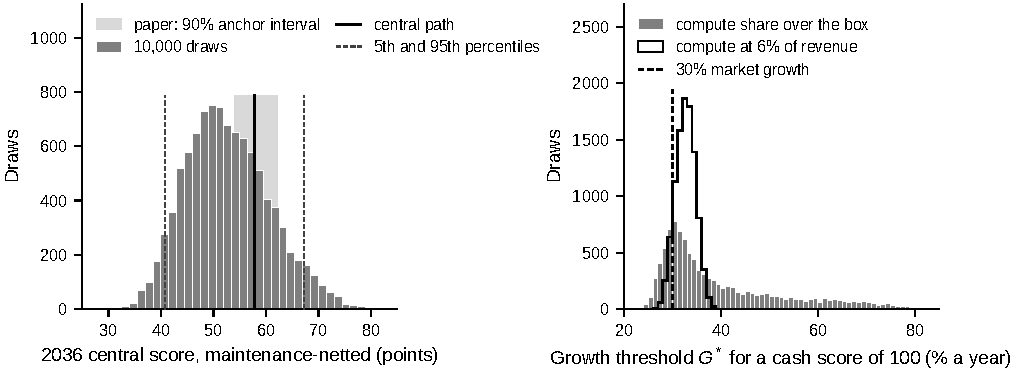
\includegraphics[width=\linewidth]{figures/fig_stress.pdf}
\caption{Joint-parameter stress test. Left: the central 2036 score on the netted basis over the \StDraws{} draws, against the paper's 90\% anchor-sampling interval; dashed lines mark the 5th and 95th percentiles of the draws. Right: the growth threshold $G^*$ for a cash score of 100, with the compute share over the box (\StCcBoxMin{} to \StCcBoxMax\% of revenue at 2025 prices) and at \CcCen\% of revenue. The draws are uniform on the stated ranges, log-uniform for compute per dollar of labor, an assumption, not a measured distribution}\label{fig:stress}
\end{figure}

% Specification curve of the empirical headline claims (round 3; reviewers GLM-M9 and GPT-16 for the two variants).
% Input by paper1/supplement.tex after sections/supp_stress.tex; paper1/spec_macros.tex is input from paper1/macros.tex
% (code/paper1_macros.py), as stress_macros.tex is. Rerun on the re-estimated sample (R2 in the main sample): log.md.
% Pre-specification: notes/spec_curve/design.md (2026-11-03 14:36 UTC, before any estimate); results:
% notes/spec_curve/results.json (code/spec_curve.py). Every number is a macro of paper1/spec_macros.tex or paper1/macros.tex;
% each qualitative statement below is tested by check_text_claims() in code/spec_curve.py, which stops if a rerun no
% longer supports it.
\clearpage
\section{A specification curve of the empirical claims}\label{supp:speccurve}
\emph{Method.} Section~\ref{sec:empirics} and Table~\ref{tab:robust} change the analysis choices one at a time. This section changes them together, in a specification curve \citep{simonsohn2020specification}, or multiverse analysis \citep{steegen2016increasing}, and asks of each headline empirical claim in how many of the resulting specifications it holds. The claims, the choices, their options and the test of each claim were written down in \texttt{notes/spec\_curve/design.md} before any estimate was computed. Only options that the paper itself uses, reports or names as defensible enter. Six choices define the sample: the treatment of acquired growth (observed growth; pro forma organic growth at acquisition flags of 10, 25 and 50\% of prior-year revenue, with ambiguous disclosures excluded, read additively or read cumulatively; exclusion of acquisition-affected years at the three flags; the two imputation bounds; \ScNAcq{} options), the sensitivities of rule R1, of rule R2 (the main sample, which applies the rule, or without the firms that both, or either, of two independent readers of the business descriptions class as not software, or without all 16 firms the review panels named), of rule R5 and of the debt-only filers, and an upper bound on growth of 500\% (the sample's) or 150\% (the bound of the fixed-effects regressions and the stochastic frontier). Crossed, they give \ScNSamples{} samples. Each claim adds its own options: the upper quantile (95th or 90th percentile) and the end period (2023--25, 2023--24 or 2025) of the decline; the frontier estimator ($\Psi_\chi$ for $\chi$ from 0.80 to 0.95, or the order-$m$ frontier) and the growth window of the slope; the period split of the steepening (2010--19 against 2020--25, or 2010--15 against 2018--25); the cash measure (the paper's, or before interest paid and cash taxes, or before interest after tax, Table~\ref{tab:bridge_v3}); and the cut-off and the treatment of acquisition-affected years in the anchor. In all there are \ScNSpecs{} specifications. The script \texttt{code/spec\_curve.py} runs the paper's own estimation code; at the \ScReproVariants{} published samples of Table~\ref{tab:robust} that lie in the grid it reproduces all \ScReproN{} stored statistics of \texttt{notes/empirics\_v3.json} that the curve uses, without difference, and \ScReproMacros{} printed values. A claim holds in a specification if the point estimate passes its test (Table~\ref{tab:spec_curve}). A firm-cluster bootstrap with \ScBootB{} replications, on all specifications of \ScBootK{} of the samples, adds the share whose 90\% interval lies on the claimed side; these intervals are not adjusted for multiplicity. The curve varies analysis choices on fixed data. The specifications share most of their firm-years, so they are not independent replications, and a share of specifications is not a probability. It tests the descriptive statements of Section~\ref{sec:empirics}, not any causal reading of them, and it does not replace the familywise corrections reported there.

\begin{table}[t]\centering\footnotesize\setlength{\tabcolsep}{3pt}
\caption{Specification curve of the empirical headline claims: in what share of the defensible analysis choices does each claim hold?}\label{tab:spec_curve}
\begin{tabular}{@{}>{\raggedright\arraybackslash}p{4.9cm}rrrrr>{\raggedright\arraybackslash}p{2.0cm}>{\raggedright\arraybackslash}p{2.4cm}@{}}\toprule
 & & \multicolumn{2}{c}{Claim holds} & & & & \\\cmidrule(lr){3-4}
Claim (test) & Specifi\-cations & point & interval & Baseline & Median & Lowest to highest & Most influential choice (range of medians)\\\midrule
Top of the score fell, GAAP: change in P95 (P90) from 2016--19 below zero, points & 4{,}320 & 97.1\% & 40.7\% & $-$11.9 & $-$6.0 & $-$14.3 to $+$2.2 & upper quantile (5.1)\\
The same, FCF after SBC & 12{,}960 & 100\% & 48.9\% & $-$12.7 & $-$7.3 & $-$14.0 to $-$0.8 & end period (3.0)\\
$\Psi$ slope, GAAP, above $-1$ & 6{,}880 & 100\% & 100\% & $-$0.22 & $-$0.39 & $-$0.62 to $-$0.15 & growth window (0.13)\\
\quad below zero &  & 100\% & 96.6\% &  &  &  & \\
\quad above $-0.5$ (our reading of ``well under a point'') &  & 84.6\% & -- &  &  &  & \\
$\Psi$ slope, FCF after SBC, above $-1$ & 19{,}200 & 100\% & 100\% & $-$0.16 & $-$0.32 & $-$0.56 to $-$0.09 & growth window (0.11)\\
\quad below zero &  & 100\% & 99.4\% &  &  &  & \\
\quad above $-0.5$ &  & 96.3\% & -- &  &  &  & \\
GAAP frontier steepened: late minus early $\Psi$ slope below zero & 5{,}040 & 96.8\% & 31.9\% & $-$0.38 & $-$0.26 & $-$0.48 to $+$0.18 & frontier estimator (0.19)\\
Cash frontier did not steepen: difference not negative (point) / interval not below zero & 14{,}320 & 58.2\% & 97.5\% & $-$0.19 & $+$0.05 & $-$0.39 to $+$0.57 & treatment of acquired growth (0.26)\\
Spend ratio between 3.0 and 3.5 (samples varied) & 720 & 73.1\% & -- & 3.02 & 3.41 & 3.00 to 3.63 & treatment of acquired growth (0.50)\\
\quad benchmark growth also varied (secondary) & 2{,}880 & 40.5\% & -- & 3.02 & 2.83 & 2.04 to 3.63 & benchmark growth (1.04)\\
Anchor: median surplus $\Pi_{lb}$ above zero (no S\&M buys growth), points & 3{,}072 & 100\% & 100\% & $+$19.5 & $+$17.2 & $+$9.4 to $+$28.1 & anchor cut-off (13.4)\\
\quad netted basis, $\Pi_{net}$, above zero & 3{,}072 & 100\% & 60.9\% & $+$12.4 & $+$12.3 & $+$3.2 to $+$26.6 & anchor cut-off (19.4)\\
\quad all S\&M buys growth, $\Pi_{ub}$ (no claim; share above zero) & 3{,}072 & 28.1\% & -- & $-$1.3 & $-$6.4 & $-$14.8 to $+$18.3 & anchor cut-off (26.3)\\
\bottomrule\end{tabular}
\par\vspace{2pt}\footnotesize\raggedright Notes: 720 samples (15 treatments of acquired growth, the R1, R2, R5 and debt-only sensitivities and two growth bounds, crossed), each with the claim's own options (Section~\ref{supp:speccurve}); a specification counts once. Specifications: those with a defined estimate (a frontier slope needs 30 firm-years at every grid point). Point: share in which the point estimate passes the test. Interval: share in which the 90\% firm-cluster percentile interval lies on the claimed side, on the specifications of 169 of the samples (the 21 of Table~\ref{tab:robust} and a seeded random draw of the others), 199 replications, firms drawn from E1. For the cash steepening the point column gives the share with a non-negative difference and the interval column the share whose interval does not lie below zero, the sense of the paper's claim. Baseline: the specification the paper prints. Most influential choice: the choice whose options' medians differ most, with that difference. Points for score changes and surpluses; slopes and the ratio as numbers. Generated by \texttt{code/spec\_curve.py}; every specification in \texttt{notes/spec\_curve/specs.csv.gz}.
\end{table}


\emph{The decline of the top.} The change in the upper quantile of the score from 2016--19 is negative in \ScTopOpShare\% of the \ScTopOpN{} GAAP specifications and in \ScTopCashShare\% of the \ScTopCashN{} cash specifications, including every specification that measures it at the 95th percentile. All \ScTopOpFailN{} GAAP specifications with a rise measure the 90th percentile in 2025 alone, the year in which the top partly recovered; among the specifications with that pair of options the change is negative in \ScTopOpPNinetyLastShare\%. The size of the decline depends on the choices more than its sign. On the GAAP basis it runs from \ScTopOpMin{} to \ScTopOpMax{} points, with a median of \ScTopOpMed{} against \ScTopOpBase{} in the baseline, and after SBC from \ScTopCashMin{} to \ScTopCashMax{} (median \ScTopCashMed, baseline \ScTopCashBase). The quantile moves the GAAP change most (medians \ScTopOpQNinetyFiveMed{} at the 95th and \ScTopOpQNinetyMed{} at the 90th percentile) and the end period the cash change. With the paper's quantile, periods and cash measure, the samples alone move the fall between \ScTopCoreFallLo{} and \ScTopCoreFallHi{} points across the two bases, against \TopFallAllLo{} to \TopFallAllHi{} in the one-at-a-time variants of Table~\ref{tab:robust}, and the baseline falls are among the largest: \ScTopOpCoreBelowBase\% of the GAAP samples and \ScTopCashCoreBelowBase\% of the cash samples fall further. An interval that excludes zero is much less robust than the sign. In the bootstrapped specifications the 90\% interval lies below zero in \ScTopOpBootShare\% on the GAAP basis and \ScTopCashBootShare\% after SBC. With the paper's quantile and periods it does so in \ScTopOpBootCoreShare\% of the bootstrapped GAAP samples and \ScTopCashBootCoreShare\% of the cash samples; at the 90th percentile it does so in \ScTopOpBootPNinetyShare\% of the GAAP specifications, and measured to 2025 alone in \ScTopOpBootLastShare\% (GAAP) and \ScTopCashBootLastShare\% (cash).

\emph{The frontier slope.} In every one of the \ScPsiOpN{} GAAP and \ScPsiCashN{} cash specifications with a defined slope, the slope of $\Psi$ lies above $-1$ and below zero (\ScPsiOpInv{} and \ScPsiCashInv{} specifications are not defined because a cell at 60\% growth falls below 30 firm-years). The magnitude the paper quotes, about a fifth of a point, lies at the flat end of the curve. The GAAP slope runs from \ScPsiOpMin{} to \ScPsiOpMax, with a median of \ScPsiOpMed{} against \ScPsiOpBase{} in the baseline, which only \ScPsiOpAboveBase\% of the specifications exceed; after SBC it runs from \ScPsiCashMin{} to \ScPsiCashMax{} (median \ScPsiCashMed, baseline \ScPsiCashBase, exceeded by \ScPsiCashAboveBase\%). Rule R2 and the growth window move it most. Dropping firms under rule R2 steepens it: on the GAAP basis the median slope is \ScPsiOpRtwoMainMed{} with the main sample's firms, \ScPsiOpRtwoNamedMed{} without the 16 named firms and \ScPsiOpRtwoEitherMed{} without the firms either reader classes as not software; and the 0--40\% window gives a median of \ScPsiOpWinFortyMed{} against \ScPsiOpWinSixtyMed{} over 0--60\%. Observed growth gives a flatter slope than the samples that remove acquired growth (medians \ScPsiOpObsMed{} and, with pro forma organic growth, \ScPsiOpProMed). With the primary statistic, $\Psi_{0.90}$ over 0--60\%, the samples alone move the GAAP slope between \ScPsiOpPrimMin{} and \ScPsiOpPrimMax{} and the cash slope between \ScPsiCashPrimMin{} and \ScPsiCashPrimMax. A slope above $-0.5$, our reading of ``well under a point'', holds in \ScPsiOpShareHalf\% of the GAAP and \ScPsiCashShareHalf\% of the cash specifications. In the bootstrapped specifications every 90\% interval lies above $-1$, and the interval lies below zero in \ScPsiOpBootNeg\% on the GAAP basis and \ScPsiCashBootNeg\% after SBC. These intervals are not adjusted for multiplicity, under which the sign does not survive at the baseline (Section~\ref{sec:empirics}), and with \ScBootB{} replications their ends are less precise than those of the paper's \BootB.

\emph{The steepening.} The GAAP frontier steepened in sign in \ScDiffOpShare\% of the \ScDiffOpN{} specifications with defined period slopes (\ScDiffOpInv{} are not defined, \ScDiffOpInvWindow{} of them because within periods the 0--60\% window is too thin, the paper's reason for using 0--40\%). The difference runs from \ScDiffOpMin{} to \ScDiffOpMax, with a median of \ScDiffOpMed{} against \ScDiffOpBase{} in the baseline. The frontier estimator moves it most: with $\Psi_{0.90}$ the difference is negative in \ScDiffOpNinetyShare\% of the specifications (median \ScDiffOpNinetyMed), with $\Psi_{0.80}$ in \ScDiffOpEightyShare\% (\ScDiffOpEightyMed) and with the order-$m$ frontier in \ScDiffOpOrderMShare\% (\ScDiffOpOrderMMed). Its 90\% interval lies below zero in only \ScDiffOpBootShare\% of the bootstrapped specifications; with $\Psi_{0.90}$ in \ScDiffOpBootNinetyShare\%, and in \ScDiffOpBootNinetySplitAShare\% with the paper's split against \ScDiffOpBootNinetySplitBShare\% with the 2010--15 against 2018--25 split. The sign of the steepening holds in most specifications; an interval that excludes zero, which the baseline has, depends on the period split and on the sample. After SBC the difference is negative in \ScDiffCashShareNeg\% of the specifications, and the sign follows the treatment of acquired growth: it is negative in \ScDiffCashNegObs\% of the specifications with observed growth, \ScDiffCashNegOrg\% of those with pro forma organic growth or without the acquisition-affected years, and \ScDiffCashNegImp\% under the imputation bounds; with the 2010--15 against 2018--25 split it is negative in \ScDiffCashNegSplitB\%. Its interval lies below zero in \ScDiffCashBootNegObs\% of the bootstrapped specifications with observed growth and \ScDiffCashBootNegOther\% of the others. The statement that the cash frontier did not steepen therefore holds, in the sense of an interval that does not lie below zero, in \ScDiffCashBootShare\% of the bootstrapped specifications; the point estimates under observed growth, like the baseline's, point to a steepening.

\emph{The spend ratio and the anchor.} The spend ratio lies between 3.0 and 3.5 (after rounding: $2.95\le$ ratio $<3.55$, the pre-specified test) in \ScSpendShare\% of the \ScSpendN{} samples and runs from \ScSpendMin{} to \ScSpendMax. It exceeds 3.5 only in samples that remove acquired growth (median \ScSpendProMed{} with pro forma organic growth against \ScSpendObsMed{} with observed growth), and mostly when firms are dropped under rule R2: the stated range holds in \ScSpendRtwoMainShare\% of the samples with the main sample's firms, \ScSpendRtwoNamedShare\% without the 16 named firms and \ScSpendRtwoEitherShare\% without the firms either reader classes as not software. With the benchmark growth varied as well, as Section~\ref{sec:empirics} does for the product $\alpha(X-k)$, the ratio runs from \ScSpendBenchMin{} to \ScSpendBenchMax, which restates the paper's point that its value depends on how excess growth is measured. The anchor's median surplus when no selling spend buys growth is positive in all \ScAncLbN{} specifications, from \ScAncLbMin{} to \ScAncLbMax{} points, and its interval lies above zero in \ScAncLbBootShare\% of those bootstrapped. The cut-off moves it most (median \ScAncLbCutNinetyMed{} at the 90th and \ScAncLbCutNinetySevenFiveMed{} at the 97.5th percentile of the cash score), since a higher cut-off selects faster-growing firm-years. On the netted basis the median surplus is positive in \ScAncNetShare\% of the specifications, with a lowest value of \ScAncNetMin{} points, and its interval lies above zero in only \ScAncNetBootShare\% of those bootstrapped: in \ScAncNetBootCutShare\% at the 95th-percentile cut-off, and in \ScAncNetBootObsDropShare\% of those with observed growth and the calibration's rule of dropping acquisition-affected years from the tail. At the baseline the interval runs from \ScAncNetBootBaseLo{} to \ScAncNetBootBaseHi{} points with \ScBootB{} replications, against \AncPiNetEoneLo{} to \AncPiNetEoneHi{} with the paper's \BootB, so its lower end lies at zero within simulation error. When all selling spend buys growth it is positive in \ScAncUbShare\% of the specifications and runs from \ScAncUbMin{} to \ScAncUbMax, so the curve, like Section~\ref{sec:empirics-anchor}, does not sign it.

\emph{Forward pairing.} Reported scores pair a year's growth with the same year's margin. Pairing each year's margin with the next year's growth instead, the model's timing, in which spend this year buys growth next year, keeps \ScFwdNEone{} of the \VNEone{} E1 firm-years (a firm's last year, and years whose successor is outside the sample, have no pair), and 2023--25 then holds only the \ScFwdLateNEone{} pairs with a 2023 or 2024 margin. Under E1 the decline is \ScFwdTopOpEone{} points on the GAAP basis and \ScFwdTopCashEone{} after SBC, against \ScTopOpBase{} and \ScTopCashBase{} with the reported pairing; the $\Psi_{0.90}$ slope is \ScFwdPsiOpEone{} and \ScFwdPsiCashEone, steeper than \PsiOpEone{} and \PsiCashEone; and the period differences are \ScFwdDiffOpEone{} and \ScFwdDiffCashEone. Under E2 the cell at 60\% growth holds \ScFwdCellEtwo{} pairs, and \ScFwdCellImpFour{} under the imputation bound at $M=4$, so the slope over 0--60\% is not defined there; the E2 decline is \ScFwdTopOpEtwo{} (GAAP) and \ScFwdTopCashEtwo{} (cash). Over the whole grid with this pairing, the decline holds in \ScFGTopOpShare\% of the \ScFGTopOpN{} GAAP and \ScFGTopCashShare\% of the \ScFGTopCashN{} cash specifications that are defined (none that ends in 2025 is), the slope lies above $-1$ and below zero in every defined specification and above $-0.5$ in \ScFGPsiOpShareHalf\% on the GAAP basis, and the GAAP difference is negative in \ScFGDiffOpShare\%. Indexing the same pairs by the year of growth, or pairing each year's growth with the next year's margin, gives GAAP changes of \ScFwdNextTopOpEone{} and \ScLagTopOpEone{} points and GAAP slopes of \ScFwdNextPsiOpEone{} and \ScLagPsiOpEone{} under E1. Under E1 no pairing changes the sign of the decline, the slope or the GAAP steepening; the pairings change their size, and the model's timing steepens the frontier slope. The cash difference keeps its negative sign with the model's timing (\ScFwdDiffCashEone) and turns positive (\ScLagDiffCashEone) when each year's growth is paired with the next year's margin.

\emph{Leave one firm out.} Dropping each of the \VFirmsEone{} firms of E1 in turn moves the GAAP decline between \ScLoTopOpEoneLo{} and \ScLoTopOpEoneHi{} points and the cash decline between \ScLoTopCashEoneLo{} and \ScLoTopCashEoneHi; the $\Psi_{0.90}$ slope between \ScLoPsiOpEoneLo{} and \ScLoPsiOpEoneHi{} (GAAP) and \ScLoPsiCashEoneLo{} and \ScLoPsiCashEoneHi{} (cash); and the GAAP steepening between \ScLoDiffOpEoneLo{} and \ScLoDiffOpEoneHi. No single firm reverses the sign of any of these five quantities, under E1, E2 or either imputation bound. The cell at 60\% growth keeps at least \ScLoCellEoneMin{} firm-years under E1 and \ScLoCellEtwoMin{} under E2, and $\phi_{0.90}$ at 60\% growth moves between \ScLoPhiOpEoneLo{} and \ScLoPhiOpEoneHi{} points of GAAP margin under E1. Single firms matter more under E2, where removing one firm shrinks the GAAP change to \ScLoTopOpEtwoHi{} points and another steepens the GAAP slope to \ScLoPsiOpEtwoLo; the cash difference, \PsiDiffCashEtwo{} under E2, keeps its sign whichever firm is removed, but under the imputation bound at $M=4$ it changes sign when one of \ScLoDiffCashReversalsImpFour{} firms is removed. For the anchor, removing any firm, not only one of the anchor's own, leaves the E1 median surplus when all selling spend buys growth within the range of \AncLooLo{} to \AncLooHi{} reported in Section~\ref{sec:empirics-anchor}, and the surplus when none does between \ScLoAncLbEoneLo{} and \ScLoAncLbEoneHi{} points.

\emph{What the curve shows.} In sign, three statements hold in every or nearly every specification: the top of the score fell between 2016--19 and 2023--25; the frontier slope lies far above $-1$ and below zero; and if selling spend does not buy growth, the best scores of 2023--25 exceed their durable level. The GAAP steepening holds in sign in \ScDiffOpShare\% of the specifications. The statement that the cash frontier did not steepen depends on the treatment of acquired growth: it describes the samples that remove acquired growth, not observed scores. Intervals that exclude zero are less robust than signs. They hold everywhere for the distance of the slope from $-1$ and in \ScAncLbBootShare\% of the bootstrapped specifications for the lower-bound surplus of the anchor, but for the decline as the paper measures it in only \ScTopOpBootCoreShare\% of the bootstrapped samples on the GAAP basis and \ScTopCashBootCoreShare\% after SBC, for the GAAP steepening in \ScDiffOpBootShare\% of the specifications and for the netted anchor surplus in \ScAncNetBootShare\%. Magnitudes are less robust than signs too. The baseline decline is among the largest that the choices produce and the baseline slope among the flattest, so ``about a fifth of a point'' describes the baseline, not the typical specification, whose slope is about \ScPsiOpMed{} on the GAAP basis; and the spend ratio leaves the range of 3.0 to 3.5, always upward and to at most \ScSpendMax, in \ScSpendShareAbove\% of the samples.

\begin{figure}[!ht]\centering
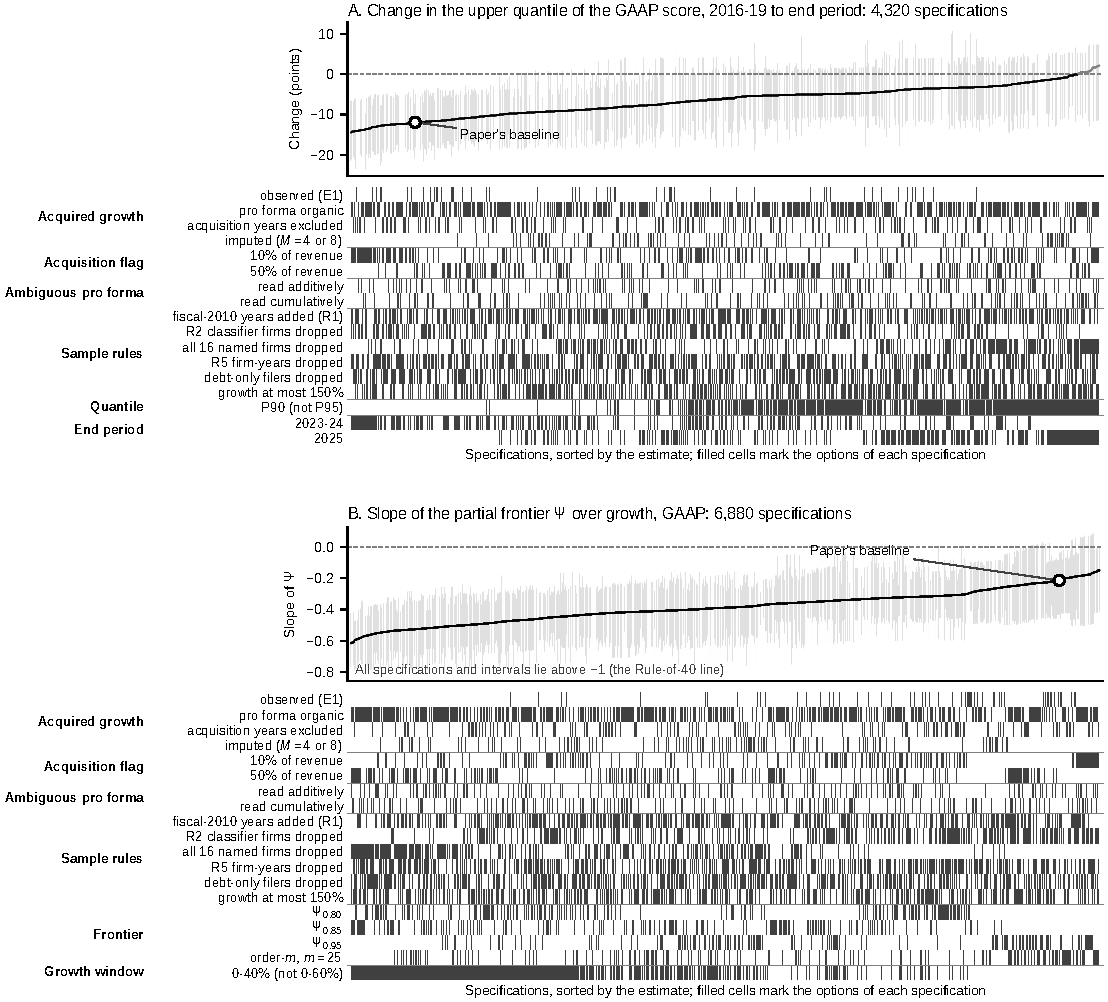
\includegraphics[width=\linewidth]{figures/fig_spec_curve.pdf}
\caption{Specification curves of two headline claims. A: change in the upper quantile of the GAAP score from 2016--19 to the end period, \ScTopOpN{} specifications sorted by the estimate; black, a decline; grey, a rise. B: slope of the partial frontier $\Psi$ over growth on the GAAP basis, \ScPsiOpN{} specifications with a defined slope. Open circles: the paper's baseline. Light vertical lines: 90\% firm-cluster percentile intervals of the specifications in the \ScBootK{} bootstrapped samples (\ScBootB{} replications). Below each curve, filled cells mark the options of each specification: every family of treatment of acquired growth, and for the other choices the options other than the paper's, so that a specification with no filled cell in a group takes the paper's option there. Generated by \texttt{code/spec\_curve.py}}\label{fig:spec_curve}
\end{figure}

\IfFileExists{sections/supp_glossary.tex}{\section{Glossary}\label{supp:glossary}
Plain-language meanings of the terms the main paper uses most. The definitions in the main paper govern where the two differ.

{\small
\begin{description}[leftmargin=0pt,itemsep=2pt]
\item[Accountability floor ($a_{\min}$).] The share of revenue that a fully automated firm still spends on being accountable: officer certifications, the integrated audit, internal control over financial reporting, insurance and legal costs. Part of it is a requirement on how controls are designed, not a headcount (\autoref{prop:amin}).
\item[Anchor.] The firm-years at or above the 95th percentile of the 2023--25 cash score, without acquisition-affected years, from which the central path starts (Section~\ref{sec:empirics-anchor}; Table~\ref{tab:anchor-firms}).
\item[Capital intensity ($k$).] Capital the firm must add per dollar of new revenue. With $k>0$ growth uses cash; with $k<0$, as when customers pay in advance, growth brings cash in.
\item[Compute share ($c_c$).] The cost of the computing that replaces labor, as a share of revenue, at full automation. A scenario value, and the largest uncertainty in the ceiling.
\item[Decision weight.] The weight a value-maximizing firm puts on a point of growth relative to a point of margin: under the verification hypothesis (H) of \autoref{prop:dynamic}, the value of an extra dollar of revenue. It depends on the owner's discount rate, and the data do not identify it.
\item[Demand pull.] How much growth a dollar of growth spend buys at a small market share; better products and channels have more of it.
\item[Durable (saturated) score.] The score a firm keeps once it has no share left to gain: its margin intercept plus market growth net of the capital that growth needs.
\item[Embedded and realized shares.] Of an automation program, the share whose processes have been changed and stay changed (embedded), and the share of the program's targeted benefits the firm actually captures (realized), which is smaller.
\item[Estimands E1 and E2.] E1 uses scores as reported; E2 removes growth bought by acquisition. The imputation bounds add back, with imputed organic growth, the acquisition years E2 cannot adjust.
\item[Familywise correction.] An adjustment of $p$-values for testing many statistics at once, so that the chance of any false finding in the family stays at the stated level.
\item[Frontier.] The best margin a firm can earn at each growth rate. The frontier estimated across firms (\autoref{def:industry}) is drawn through the points firms chose, not through any one firm's possibilities.
\item[Full-automation ceiling ($R_{\max}$).] The highest durable cash score a firm can reach at a stated full-automation cost structure and fixed prices (\autoref{cor:ceiling}). A bound at that cost structure, not a forecast or a target.
\item[Full-cost floors.] The recurring costs of running AI that full automation adds: maintaining, securing and supervising it, and the losses its errors cause (\autoref{def:fullcost}).
\item[Growth surplus ($\Pi$).] The part of a score above its durable level, earned while the firm still has share to gain. It is transient.
\item[Margin intercept ($m_0$).] The margin a firm would earn if it spent nothing to grow faster than its market.
\item[Market growth ($G$).] How fast the firm's whole market grows; a firm can match it without growth spend.
\item[Pass-through.] The share of a fall in unit costs that competition passes to customers as lower prices.
\item[Price line.] A Rule-of-40 or Rule-of-$X$ line: its slope is the number of margin points the rule trades for one point of growth. Firms on the same line have the same score, not the same value.
\item[$\Psi_\chi$.] The paper's primary frontier statistic: for each growth level, the $\chi$-quantile of the margin among firm-years that grew at least that fast.
\item[Remote threshold ($\bar\pi$).] In the control model, the largest probability that a design may leave that, over the year's opportunities for a material misstatement, at least one passes every control layer. A scenario value, not a tolerance.
\item[Screening weight.] The weight on growth that investors use to compare firms, typically two to three; it reflects how long growth lasts.
\item[Share headroom and the score budget.] The room a firm has to gain share in its market. Within one market and at given retention, every point of score above the durable level uses up part of a finite budget of headroom (\autoref{prop:budget}).
\item[Spend elasticity ($\alpha$).] How fast the returns to growth spend diminish; the data do not identify it, so the paper uses a range.
\item[Top-tail firm.] A firm at the 95th percentile of the 2023--25 cash score, the starting point of the central path.
\item[$T(g_0)$.] The 95th-percentile margin among firm-years growing at least $g_0$, plus $g_0$: a point on the frontier at a fixed growth rate.
\end{description}
}
}{}

{\footnotesize\setstretch{1.0}
\setlength{\bibsep}{1pt plus 1pt}
\bibliographystyle{plainnat_p1}
\bibliography{paper1/refs_paper1}
}
\end{document}
